% This is some page header magic to get part titles in the header. -gmm 2010/02/03
% http://newsgroups.derkeiler.com/Archive/Comp/comp.text.tex/2005-12/msg00686.html
\copypagestyle{cmb}{headings} 
\makepsmarks{cmb}{% 
	\renewcommand\sectionmark[1]{} 
	\renewcommand\partmark[1]{\markboth{\textit{##1}}{}} 
	\renewcommand\chaptermark[1]{\markright{\thechapter. ##1}}% 
} 
\makeheadposition{cmb}{flushright}{flushleft}{flushright}{flushleft} 
\makeoddhead{cmb}{\leftmark}{}{\thepage} 
\makeevenhead{cmb}{\thepage}{}{\textit{The Adventures of @SHERLOCK_HOLMES_FIRSTNAME@ @SHERLOCK_HOLMES_LASTNAME@}}

\pagestyle{cmb}

\book*{The Adventures of @SHERLOCK_HOLMES_FIRSTNAME@ @SHERLOCK_HOLMES_LASTNAME@ by Sir Arthur Conan Doyle}

\cleardoublepage

\frontmatter

\maxtocdepth{part}
\settocdepth{part}
\cftsetindents{part}{0em}{3em}
\setlength{\cftbeforepartskip}{1.5em}

\clearpage
\tableofcontents
\clearpage

\pagestyle{empty}
\begin{figure}
	\centering
	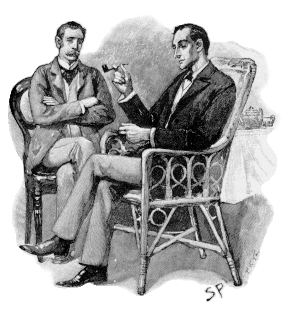
\includegraphics[width=2in]{paget_holmes.png}
\end{figure}

\mainmatter
\pagestyle{cmb}

\part{A Scandal in Bohemia}

\chapter*{I}

To @SHERLOCK_HOLMES_FIRSTNAME@ @SHERLOCK_HOLMES_LASTNAME@ she is always \textit{the} woman. I have seldom heard
him mention her under any other name. In his eyes she eclipses
and predominates the whole of her sex. It was not that he felt
any emotion akin to love for @IRENE_ADLER_FIRSTNAME@ @IRENE_ADLER_LASTNAME@. All emotions, and that
one particularly, were abhorrent to his cold, precise but
admirably balanced mind. He was, I take it, the most perfect
reasoning and observing machine that the world has seen, but as a
lover he would have placed himself in a false position. He never
spoke of the softer passions, save with a gibe and a sneer. They
were admirable things for the observer--excellent for drawing the
veil from men's motives and actions. But for the trained reasoner
to admit such intrusions into his own delicate and finely
adjusted temperament was to introduce a distracting factor which
might throw a doubt upon all his mental results. Grit in a
sensitive instrument, or a crack in one of his own high-power
lenses, would not be more disturbing than a strong emotion in a
nature such as his. And yet there was but one woman to him, and
that woman was the late @IRENE_ADLER_FIRSTNAME@ @IRENE_ADLER_LASTNAME@, of dubious and questionable
memory.

I had seen little of @SHERLOCK_HOLMES_LASTNAME@ lately. My marriage had drifted us
away from each other. My own complete happiness, and the
home-centred interests which rise up around the man who first
finds himself master of his own establishment, were sufficient to
absorb all my attention, while @SHERLOCK_HOLMES_LASTNAME@, who loathed every form of
society with his whole Bohemian soul, remained in our lodgings in
@BAKER_STREET_NAME@, buried among his old books, and alternating from
week to week between cocaine and ambition, the drowsiness of the
drug, and the fierce energy of his own keen nature. He was still,
as ever, deeply attracted by the study of crime, and occupied his
immense faculties and extraordinary powers of observation in
following out those clues, and clearing up those mysteries which
had been abandoned as hopeless by the official police. From time
to time I heard some vague account of his doings: of his summons
to Odessa in the case of the Trepoff murder, of his clearing up
of the singular tragedy of the Atkinson brothers at Trincomalee,
and finally of the mission which he had accomplished so
delicately and successfully for the reigning family of Holland.
Beyond these signs of his activity, however, which I merely
shared with all the readers of the daily press, I knew little of
my former friend and companion.

One night--it was on the twentieth of March, 1888--I was
returning from a journey to a patient (for I had now returned to
civil practice), when my way led me through @BAKER_STREET_NAME@. As I
passed the well-remembered door, which must always be associated
in my mind with my wooing, and with the dark incidents of the
Study in Scarlet, I was seized with a keen desire to see @SHERLOCK_HOLMES_LASTNAME@
again, and to know how he was employing his extraordinary powers.
His rooms were brilliantly lit, and, even as I looked up, I saw
his tall, spare figure pass twice in a dark silhouette against
the blind. He was pacing the room swiftly, eagerly, with his head
sunk upon his chest and his hands clasped behind him. To me, who
knew his every mood and habit, his attitude and manner told their
own story. He was at work again. He had risen out of his
drug-created dreams and was hot upon the scent of some new
problem. I rang the bell and was shown up to the chamber which
had formerly been in part my own.

His manner was not effusive. It seldom was; but he was glad, I
think, to see me. With hardly a word spoken, but with a kindly
eye, he waved me to an armchair, threw across his case of cigars,
and indicated a spirit case and a gasogene in the corner. Then he
stood before the fire and looked me over in his singular
introspective fashion.

``Wedlock suits you,'' he remarked. ``I think, @WATSON_LASTNAME@, that you have
put on seven and a half pounds since I saw you.''

``Seven!'' I answered.

``Indeed, I should have thought a little more. Just a trifle more,
I fancy, @WATSON_LASTNAME@. And in practice again, I observe. You did not
tell me that you intended to go into harness.''

``Then, how do you know?''

``I see it, I deduce it. How do I know that you have been getting
yourself very wet lately, and that you have a most clumsy and
careless servant girl?''

``My dear @SHERLOCK_HOLMES_LASTNAME@,'' said I, ``this is too much. You would certainly
have been burned, had you lived a few centuries ago. It is true
that I had a country walk on Thursday and came home in a dreadful
mess, but as I have changed my clothes I can't imagine how you
deduce it. As to Mary Jane, she is incorrigible, and my wife has
given her notice, but there, again, I fail to see how you work it
out.''

He chuckled to himself and rubbed his long, nervous hands
together.

``It is simplicity itself,'' said he; ``my eyes tell me that on the
inside of your left shoe, just where the firelight strikes it,
the leather is scored by six almost parallel cuts. Obviously they
have been caused by someone who has very carelessly scraped round
the edges of the sole in order to remove crusted mud from it.
Hence, you see, my double deduction that you had been out in vile
weather, and that you had a particularly malignant boot-slitting
specimen of the London slavey. As to your practice, if a
gentleman walks into my rooms smelling of iodoform, with a black
mark of nitrate of silver upon his right forefinger, and a bulge
on the right side of his top-hat to show where he has secreted
his stethoscope, I must be dull, indeed, if I do not pronounce
him to be an active member of the medical profession.''

I could not help laughing at the ease with which he explained his
process of deduction. ``When I hear you give your reasons,'' I
remarked, ``the thing always appears to me to be so ridiculously
simple that I could easily do it myself, though at each
successive instance of your reasoning I am baffled until you
explain your process. And yet I believe that my eyes are as good
as yours.''

``Quite so,'' he answered, lighting a cigarette, and throwing
himself down into an armchair. ``You see, but you do not observe.
The distinction is clear. For example, you have frequently seen
the steps which lead up from the hall to this room.''

``Frequently.''

``How often?''

``Well, some hundreds of times.''

``Then how many are there?''

``How many? I don't know.''

``Quite so! You have not observed. And yet you have seen. That is
just my point. Now, I know that there are seventeen steps,
because I have both seen and observed. By-the-way, since you are
interested in these little problems, and since you are good
enough to chronicle one or two of my trifling experiences, you
may be interested in this.'' He threw over a sheet of thick,
pink-tinted note-paper which had been lying open upon the table.
``It came by the last post,'' said he. ``Read it aloud.''

The note was undated, and without either signature or address.

``There will call upon you to-night, at a quarter to eight
o'clock,'' it said, ``a gentleman who desires to consult you upon a
matter of the very deepest moment. Your recent services to one of
the royal houses of Europe have shown that you are one who may
safely be trusted with matters which are of an importance which
can hardly be exaggerated. This account of you we have from all
quarters received. Be in your chamber then at that hour, and do
not take it amiss if your visitor wear a mask.''

``This is indeed a mystery,'' I remarked. ``What do you imagine that
it means?''

``I have no data yet. It is a capital mistake to theorize before
one has data. Insensibly one begins to twist facts to suit
theories, instead of theories to suit facts. But the note itself.
What do you deduce from it?''

I carefully examined the writing, and the paper upon which it was
written.

``The man who wrote it was presumably well to do,'' I remarked,
endeavouring to imitate my companion's processes. ``Such paper
could not be bought under half a crown a packet. It is peculiarly
strong and stiff.''

``Peculiar--that is the very word,'' said @SHERLOCK_HOLMES_LASTNAME@. ``It is not an
English paper at all. Hold it up to the light.''

I did so, and saw a large ``E'' with a small ``g,'' a ``P,'' and a
large ``G'' with a small ``t'' woven into the texture of the paper.

``What do you make of that?'' asked @SHERLOCK_HOLMES_LASTNAME@.

``The name of the maker, no doubt; or his monogram, rather.''

``Not at all. The 'G' with the small 't' stands for
'Gesellschaft,' which is the German for 'Company.' It is a
customary contraction like our 'Co.' 'P,' of course, stands for
'Papier.' Now for the 'Eg.' Let us glance at our Continental
Gazetteer.'' He took down a heavy brown volume from his shelves.
``Eglow, Eglonitz--here we are, Egria. It is in a German-speaking
country--in Bohemia, not far from Carlsbad. 'Remarkable as being
the scene of the death of Wallenstein, and for its numerous
glass-factories and paper-mills.' Ha, ha, my boy, what do you
make of that?'' His eyes sparkled, and he sent up a great blue
triumphant cloud from his cigarette.

``The paper was made in Bohemia,'' I said.

``Precisely. And the man who wrote the note is a German. Do you
note the peculiar construction of the sentence--'This account of
you we have from all quarters received.' A Frenchman or Russian
could not have written that. It is the German who is so
uncourteous to his verbs. It only remains, therefore, to discover
what is wanted by this German who writes upon Bohemian paper and
prefers wearing a mask to showing his face. And here he comes, if
I am not mistaken, to resolve all our doubts.''

As he spoke there was the sharp sound of horses' hoofs and
grating wheels against the curb, followed by a sharp pull at the
bell. @SHERLOCK_HOLMES_LASTNAME@ whistled.

``A pair, by the sound,'' said he. ``Yes,'' he continued, glancing
out of the window. ``A nice little brougham and a pair of
beauties. A hundred and fifty guineas apiece. There's money in
this case, @WATSON_LASTNAME@, if there is nothing else.''

``I think that I had better go, @SHERLOCK_HOLMES_LASTNAME@.''

``Not a bit, Doctor. Stay where you are. I am lost without my
Boswell. And this promises to be interesting. It would be a pity
to miss it.''

``But your client--''

``Never mind him. I may want your help, and so may he. Here he
comes. Sit down in that armchair, Doctor, and give us your best
attention.''

A slow and heavy step, which had been heard upon the stairs and
in the passage, paused immediately outside the door. Then there
was a loud and authoritative tap.

``Come in!'' said @SHERLOCK_HOLMES_LASTNAME@.

A man entered who could hardly have been less than six feet six
inches in height, with the chest and limbs of a Hercules. His
dress was rich with a richness which would, in England, be looked
upon as akin to bad taste. Heavy bands of astrakhan were slashed
across the sleeves and fronts of his double-breasted coat, while
the deep blue cloak which was thrown over his shoulders was lined
with flame-coloured silk and secured at the neck with a brooch
which consisted of a single flaming beryl. Boots which extended
halfway up his calves, and which were trimmed at the tops with
rich brown fur, completed the impression of barbaric opulence
which was suggested by his whole appearance. He carried a
broad-brimmed hat in his hand, while he wore across the upper
part of his face, extending down past the cheekbones, a black
vizard mask, which he had apparently adjusted that very moment,
for his hand was still raised to it as he entered. From the lower
part of the face he appeared to be a man of strong character,
with a thick, hanging lip, and a long, straight chin suggestive
of resolution pushed to the length of obstinacy.

``You had my note?'' he asked with a deep harsh voice and a
strongly marked German accent. ``I told you that I would call.'' He
looked from one to the other of us, as if uncertain which to
address.

``Pray take a seat,'' said @SHERLOCK_HOLMES_LASTNAME@. ``This is my friend and
colleague, Dr. @WATSON_LASTNAME@, who is occasionally good enough to help me
in my cases. Whom have I the honour to address?''

``You may address me as the Count Von Kramm, a Bohemian nobleman.
I understand that this gentleman, your friend, is a man of honour
and discretion, whom I may trust with a matter of the most
extreme importance. If not, I should much prefer to communicate
with you alone.''

I rose to go, but @SHERLOCK_HOLMES_LASTNAME@ caught me by the wrist and pushed me
back into my chair. ``It is both, or none,'' said he. ``You may say
before this gentleman anything which you may say to me.''

The Count shrugged his broad shoulders. ``Then I must begin,'' said
he, ``by binding you both to absolute secrecy for two years; at
the end of that time the matter will be of no importance. At
present it is not too much to say that it is of such weight it
may have an influence upon European history.''

``I promise,'' said @SHERLOCK_HOLMES_LASTNAME@.

``And I.''

``You will excuse this mask,'' continued our strange visitor. ``The
august person who employs me wishes his agent to be unknown to
you, and I may confess at once that the title by which I have
just called myself is not exactly my own.''

``I was aware of it,'' said @SHERLOCK_HOLMES_LASTNAME@ dryly.

``The circumstances are of great delicacy, and every precaution
has to be taken to quench what might grow to be an immense
scandal and seriously compromise one of the reigning families of
Europe. To speak plainly, the matter implicates the great House
of Ormstein, hereditary kings of Bohemia.''

``I was also aware of that,'' murmured @SHERLOCK_HOLMES_LASTNAME@, settling himself
down in his armchair and closing his eyes.

Our visitor glanced with some apparent surprise at the languid,
lounging figure of the man who had been no doubt depicted to him
as the most incisive reasoner and most energetic agent in Europe.
@SHERLOCK_HOLMES_LASTNAME@ slowly reopened his eyes and looked impatiently at his
gigantic client.

``If your Majesty would condescend to state your case,'' he
remarked, ``I should be better able to advise you.''

The man sprang from his chair and paced up and down the room in
uncontrollable agitation. Then, with a gesture of desperation, he
tore the mask from his face and hurled it upon the ground. ``You
are right,'' he cried; ``I am the King. Why should I attempt to
conceal it?''

``Why, indeed?'' murmured @SHERLOCK_HOLMES_LASTNAME@. ``Your Majesty had not spoken
before I was aware that I was addressing Wilhelm Gottsreich
Sigismond von Ormstein, Grand Duke of Cassel-Felstein, and
hereditary King of Bohemia.''

``But you can understand,'' said our strange visitor, sitting down
once more and passing his hand over his high white forehead, ``you
can understand that I am not accustomed to doing such business in
my own person. Yet the matter was so delicate that I could not
confide it to an agent without putting myself in his power. I
have come incognito from Prague for the purpose of consulting
you.''

``Then, pray consult,'' said @SHERLOCK_HOLMES_LASTNAME@, shutting his eyes once more.

``The facts are briefly these: Some five years ago, during a
lengthy visit to Warsaw, I made the acquaintance of the well-known
adventuress, @IRENE_ADLER_FIRSTNAME@ @IRENE_ADLER_LASTNAME@. The name is no doubt familiar to you.''

``Kindly look her up in my index, Doctor,'' murmured @SHERLOCK_HOLMES_LASTNAME@ without
opening his eyes. For many years he had adopted a system of
docketing all paragraphs concerning men and things, so that it
was difficult to name a subject or a person on which he could not
at once furnish information. In this case I found her biography
sandwiched in between that of a Hebrew rabbi and that of a
staff-commander who had written a monograph upon the deep-sea
fishes.

``Let me see!'' said @SHERLOCK_HOLMES_LASTNAME@. ``Hum! Born in New Jersey in the year
1858. Contralto--hum! La Scala, hum! Prima donna Imperial Opera
of Warsaw--yes! Retired from operatic stage--ha! Living in
London--quite so! Your Majesty, as I understand, became entangled
with this young person, wrote her some compromising letters, and
is now desirous of getting those letters back.''

``Precisely so. But how--''

``Was there a secret marriage?''

``None.''

``No legal papers or certificates?''

``None.''

``Then I fail to follow your Majesty. If this young person should
produce her letters for blackmailing or other purposes, how is
she to prove their authenticity?''

``There is the writing.''

``Pooh, pooh! Forgery.''

``My private note-paper.''

``Stolen.''

``My own seal.''

``Imitated.''

``My photograph.''

``Bought.''

``We were both in the photograph.''

``Oh, dear! That is very bad! Your Majesty has indeed committed an
indiscretion.''

``I was mad--insane.''

``You have compromised yourself seriously.''

``I was only Crown Prince then. I was young. I am but thirty now.''

``It must be recovered.''

``We have tried and failed.''

``Your Majesty must pay. It must be bought.''

``She will not sell.''

``Stolen, then.''

``Five attempts have been made. Twice burglars in my pay ransacked
her house. Once we diverted her luggage when she travelled. Twice
she has been waylaid. There has been no result.''

``No sign of it?''

``Absolutely none.''

@SHERLOCK_HOLMES_LASTNAME@ laughed. ``It is quite a pretty little problem,'' said he.

``But a very serious one to me,'' returned the King reproachfully.

``Very, indeed. And what does she propose to do with the
photograph?''

``To ruin me.''

``But how?''

``I am about to be married.''

``So I have heard.''

``To Clotilde Lothman von Saxe-Meningen, second daughter of the
King of Scandinavia. You may know the strict principles of her
family. She is herself the very soul of delicacy. A shadow of a
doubt as to my conduct would bring the matter to an end.''

``And @IRENE_ADLER_FIRSTNAME@ @IRENE_ADLER_LASTNAME@?''

``Threatens to send them the photograph. And she will do it. I
know that she will do it. You do not know her, but she has a soul
of steel. She has the face of the most beautiful of women, and
the mind of the most resolute of men. Rather than I should marry
another woman, there are no lengths to which she would not
go--none.''

``You are sure that she has not sent it yet?''

``I am sure.''

``And why?''

``Because she has said that she would send it on the day when the
betrothal was publicly proclaimed. That will be next Monday.''

``Oh, then we have three days yet,'' said @SHERLOCK_HOLMES_LASTNAME@ with a yawn. ``That
is very fortunate, as I have one or two matters of importance to
look into just at present. Your Majesty will, of course, stay in
London for the present?''

``Certainly. You will find me at the Langham under the name of the
Count Von Kramm.''

``Then I shall drop you a line to let you know how we progress.''

``Pray do so. I shall be all anxiety.''

``Then, as to money?''

``You have carte blanche.''

``Absolutely?''

``I tell you that I would give one of the provinces of my kingdom
to have that photograph.''

``And for present expenses?''

The King took a heavy chamois leather bag from under his cloak
and laid it on the table.

``There are three hundred pounds in gold and seven hundred in
notes,'' he said.

@SHERLOCK_HOLMES_LASTNAME@ scribbled a receipt upon a sheet of his note-book and
handed it to him.

``And Mademoiselle's address?'' he asked.

``Is Briony Lodge, Serpentine Avenue, St. John's Wood.''

@SHERLOCK_HOLMES_LASTNAME@ took a note of it. ``One other question,'' said he. ``Was the
photograph a cabinet?''

``It was.''

``Then, good-night, your Majesty, and I trust that we shall soon
have some good news for you. And good-night, @WATSON_LASTNAME@,'' he added,
as the wheels of the royal brougham rolled down the street. ``If
you will be good enough to call to-morrow afternoon at three
o'clock I should like to chat this little matter over with you.''


\chapter*{II}

At three o'clock precisely I was at @BAKER_STREET_NAME@, but @SHERLOCK_HOLMES_LASTNAME@ had
not yet returned. The landlady informed me that he had left the
house shortly after eight o'clock in the morning. I sat down
beside the fire, however, with the intention of awaiting him,
however long he might be. I was already deeply interested in his
inquiry, for, though it was surrounded by none of the grim and
strange features which were associated with the two crimes which
I have already recorded, still, the nature of the case and the
exalted station of his client gave it a character of its own.
Indeed, apart from the nature of the investigation which my
friend had on hand, there was something in his masterly grasp of
a situation, and his keen, incisive reasoning, which made it a
pleasure to me to study his system of work, and to follow the
quick, subtle methods by which he disentangled the most
inextricable mysteries. So accustomed was I to his invariable
success that the very possibility of his failing had ceased to
enter into my head.

It was close upon four before the door opened, and a
drunken-looking groom, ill-kempt and side-whiskered, with an
inflamed face and disreputable clothes, walked into the room.
Accustomed as I was to my friend's amazing powers in the use of
disguises, I had to look three times before I was certain that it
was indeed he. With a nod he vanished into the bedroom, whence he
emerged in five minutes tweed-suited and respectable, as of old.
Putting his hands into his pockets, he stretched out his legs in
front of the fire and laughed heartily for some minutes.

``Well, really!'' he cried, and then he choked and laughed again
until he was obliged to lie back, limp and helpless, in the
chair.

``What is it?''

``It's quite too funny. I am sure you could never guess how I
employed my morning, or what I ended by doing.''

``I can't imagine. I suppose that you have been watching the
habits, and perhaps the house, of Miss @IRENE_ADLER_FIRSTNAME@ @IRENE_ADLER_LASTNAME@.''

``Quite so; but the sequel was rather unusual. I will tell you,
however. I left the house a little after eight o'clock this
morning in the character of a groom out of work. There is a
wonderful sympathy and freemasonry among horsey men. Be one of
them, and you will know all that there is to know. I soon found
Briony Lodge. It is a bijou villa, with a garden at the back, but
built out in front right up to the road, two stories. Chubb lock
to the door. Large sitting-room on the right side, well
furnished, with long windows almost to the floor, and those
preposterous English window fasteners which a child could open.
Behind there was nothing remarkable, save that the passage window
could be reached from the top of the coach-house. I walked round
it and examined it closely from every point of view, but without
noting anything else of interest.

``I then lounged down the street and found, as I expected, that
there was a mews in a lane which runs down by one wall of the
garden. I lent the ostlers a hand in rubbing down their horses,
and received in exchange twopence, a glass of half and half, two
fills of shag tobacco, and as much information as I could desire
about Miss @IRENE_ADLER_LASTNAME@, to say nothing of half a dozen other people in
the neighbourhood in whom I was not in the least interested, but
whose biographies I was compelled to listen to.''

``And what of @IRENE_ADLER_FIRSTNAME@ @IRENE_ADLER_LASTNAME@?'' I asked.

``Oh, she has turned all the men's heads down in that part. She is
the daintiest thing under a bonnet on this planet. So say the
Serpentine-mews, to a man. She lives quietly, sings at concerts,
drives out at five every day, and returns at seven sharp for
dinner. Seldom goes out at other times, except when she sings.
Has only one male visitor, but a good deal of him. He is dark,
handsome, and dashing, never calls less than once a day, and
often twice. He is a Mr. Godfrey Norton, of the Inner Temple. See
the advantages of a cabman as a confidant. They had driven him
home a dozen times from Serpentine-mews, and knew all about him.
When I had listened to all they had to tell, I began to walk up
and down near Briony Lodge once more, and to think over my plan
of campaign.

``This Godfrey Norton was evidently an important factor in the
matter. He was a lawyer. That sounded ominous. What was the
relation between them, and what the object of his repeated
visits? Was she his client, his friend, or his mistress? If the
former, she had probably transferred the photograph to his
keeping. If the latter, it was less likely. On the issue of this
question depended whether I should continue my work at Briony
Lodge, or turn my attention to the gentleman's chambers in the
Temple. It was a delicate point, and it widened the field of my
inquiry. I fear that I bore you with these details, but I have to
let you see my little difficulties, if you are to understand the
situation.''

``I am following you closely,'' I answered.

``I was still balancing the matter in my mind when a hansom cab
drove up to Briony Lodge, and a gentleman sprang out. He was a
remarkably handsome man, dark, aquiline, and moustached--
evidently the man of whom I had heard. He appeared to be in a
great hurry, shouted to the cabman to wait, and brushed past the
maid who opened the door with the air of a man who was thoroughly
at home.

``He was in the house about half an hour, and I could catch
glimpses of him in the windows of the sitting-room, pacing up and
down, talking excitedly, and waving his arms. Of her I could see
nothing. Presently he emerged, looking even more flurried than
before. As he stepped up to the cab, he pulled a gold watch from
his pocket and looked at it earnestly, 'Drive like the devil,' he
shouted, 'first to Gross \& Hankey's in Regent Street, and then to
the Church of St. Monica in the Edgeware Road. Half a guinea if
you do it in twenty minutes!'

``Away they went, and I was just wondering whether I should not do
well to follow them when up the lane came a neat little landau,
the coachman with his coat only half-buttoned, and his tie under
his ear, while all the tags of his harness were sticking out of
the buckles. It hadn't pulled up before she shot out of the hall
door and into it. I only caught a glimpse of her at the moment,
but she was a lovely woman, with a face that a man might die for.

``'The Church of St. Monica, John,' she cried, 'and half a
sovereign if you reach it in twenty minutes.'

``This was quite too good to lose, @WATSON_LASTNAME@. I was just balancing
whether I should run for it, or whether I should perch behind her
landau when a cab came through the street. The driver looked
twice at such a shabby fare, but I jumped in before he could
object. 'The Church of St. Monica,' said I, 'and half a sovereign
if you reach it in twenty minutes.' It was twenty-five minutes to
twelve, and of course it was clear enough what was in the wind.

``My cabby drove fast. I don't think I ever drove faster, but the
others were there before us. The cab and the landau with their
steaming horses were in front of the door when I arrived. I paid
the man and hurried into the church. There was not a soul there
save the two whom I had followed and a surpliced clergyman, who
seemed to be expostulating with them. They were all three
standing in a knot in front of the altar. I lounged up the side
aisle like any other idler who has dropped into a church.
Suddenly, to my surprise, the three at the altar faced round to
me, and Godfrey Norton came running as hard as he could towards
me.

``'Thank God,' he cried. 'You'll do. Come! Come!'

``'What then?' I asked.

``'Come, man, come, only three minutes, or it won't be legal.'

``I was half-dragged up to the altar, and before I knew where I was
I found myself mumbling responses which were whispered in my ear,
and vouching for things of which I knew nothing, and generally
assisting in the secure tying up of @IRENE_ADLER_FIRSTNAME@ @IRENE_ADLER_LASTNAME@, spinster, to
Godfrey Norton, bachelor. It was all done in an instant, and
there was the gentleman thanking me on the one side and the lady
on the other, while the clergyman beamed on me in front. It was
the most preposterous position in which I ever found myself in my
life, and it was the thought of it that started me laughing just
now. It seems that there had been some informality about their
license, that the clergyman absolutely refused to marry them
without a witness of some sort, and that my lucky appearance
saved the bridegroom from having to sally out into the streets in
search of a best man. The bride gave me a sovereign, and I mean
to wear it on my watch-chain in memory of the occasion.''

``This is a very unexpected turn of affairs,'' said I; ``and what
then?''

``Well, I found my plans very seriously menaced. It looked as if
the pair might take an immediate departure, and so necessitate
very prompt and energetic measures on my part. At the church
door, however, they separated, he driving back to the Temple, and
she to her own house. 'I shall drive out in the park at five as
usual,' she said as she left him. I heard no more. They drove
away in different directions, and I went off to make my own
arrangements.''

``Which are?''

``Some cold beef and a glass of beer,'' he answered, ringing the
bell. ``I have been too busy to think of food, and I am likely to
be busier still this evening. By the way, Doctor, I shall want
your co-operation.''

``I shall be delighted.''

``You don't mind breaking the law?''

``Not in the least.''

``Nor running a chance of arrest?''

``Not in a good cause.''

``Oh, the cause is excellent!''

``Then I am your man.''

``I was sure that I might rely on you.''

``But what is it you wish?''

``When Mrs. Turner has brought in the tray I will make it clear to
you. Now,'' he said as he turned hungrily on the simple fare that
our landlady had provided, ``I must discuss it while I eat, for I
have not much time. It is nearly five now. In two hours we must
be on the scene of action. Miss @IRENE_ADLER_FIRSTNAME@, or Madame, rather, returns
from her drive at seven. We must be at Briony Lodge to meet her.''

``And what then?''

``You must leave that to me. I have already arranged what is to
occur. There is only one point on which I must insist. You must
not interfere, come what may. You understand?''

``I am to be neutral?''

``To do nothing whatever. There will probably be some small
unpleasantness. Do not join in it. It will end in my being
conveyed into the house. Four or five minutes afterwards the
sitting-room window will open. You are to station yourself close
to that open window.''

``Yes.''

``You are to watch me, for I will be visible to you.''

``Yes.''

``And when I raise my hand--so--you will throw into the room what
I give you to throw, and will, at the same time, raise the cry of
fire. You quite follow me?''

``Entirely.''

``It is nothing very formidable,'' he said, taking a long cigar-
shaped roll from his pocket. ``It is an ordinary plumber's smoke-
rocket, fitted with a cap at either end to make it self-lighting.
Your task is confined to that. When you raise your cry of fire,
it will be taken up by quite a number of people. You may then
walk to the end of the street, and I will rejoin you in ten
minutes. I hope that I have made myself clear?''

``I am to remain neutral, to get near the window, to watch you,
and at the signal to throw in this object, then to raise the cry
of fire, and to wait you at the corner of the street.''

``Precisely.''

``Then you may entirely rely on me.''

``That is excellent. I think, perhaps, it is almost time that I
prepare for the new role I have to play.''

He disappeared into his bedroom and returned in a few minutes in
the character of an amiable and simple-minded Nonconformist
clergyman. His broad black hat, his baggy trousers, his white
tie, his sympathetic smile, and general look of peering and
benevolent curiosity were such as Mr. John Hare alone could have
equalled. It was not merely that @SHERLOCK_HOLMES_LASTNAME@ changed his costume. His
expression, his manner, his very soul seemed to vary with every
fresh part that he assumed. The stage lost a fine actor, even as
science lost an acute reasoner, when he became a specialist in
crime.

It was a quarter past six when we left @BAKER_STREET_NAME@, and it still
wanted ten minutes to the hour when we found ourselves in
Serpentine Avenue. It was already dusk, and the lamps were just
being lighted as we paced up and down in front of Briony Lodge,
waiting for the coming of its occupant. The house was just such
as I had pictured it from @SHERLOCK_HOLMES_FIRSTNAME@ @SHERLOCK_HOLMES_LASTNAME@' succinct description,
but the locality appeared to be less private than I expected. On
the contrary, for a small street in a quiet neighbourhood, it was
remarkably animated. There was a group of shabbily dressed men
smoking and laughing in a corner, a scissors-grinder with his
wheel, two guardsmen who were flirting with a nurse-girl, and
several well-dressed young men who were lounging up and down with
cigars in their mouths.

``You see,'' remarked @SHERLOCK_HOLMES_LASTNAME@, as we paced to and fro in front of
the house, ``this marriage rather simplifies matters. The
photograph becomes a double-edged weapon now. The chances are
that she would be as averse to its being seen by Mr. Godfrey
Norton, as our client is to its coming to the eyes of his
princess. Now the question is, Where are we to find the
photograph?''

``Where, indeed?''

``It is most unlikely that she carries it about with her. It is
cabinet size. Too large for easy concealment about a woman's
dress. She knows that the King is capable of having her waylaid
and searched. Two attempts of the sort have already been made. We
may take it, then, that she does not carry it about with her.''

``Where, then?''

``Her banker or her lawyer. There is that double possibility. But
I am inclined to think neither. Women are naturally secretive,
and they like to do their own secreting. Why should she hand it
over to anyone else? She could trust her own guardianship, but
she could not tell what indirect or political influence might be
brought to bear upon a business man. Besides, remember that she
had resolved to use it within a few days. It must be where she
can lay her hands upon it. It must be in her own house.''

``But it has twice been burgled.''

``Pshaw! They did not know how to look.''

``But how will you look?''

``I will not look.''

``What then?''

``I will get her to show me.''

``But she will refuse.''

``She will not be able to. But I hear the rumble of wheels. It is
her carriage. Now carry out my orders to the letter.''

As he spoke the gleam of the side-lights of a carriage came round
the curve of the avenue. It was a smart little landau which
rattled up to the door of Briony Lodge. As it pulled up, one of
the loafing men at the corner dashed forward to open the door in
the hope of earning a copper, but was elbowed away by another
loafer, who had rushed up with the same intention. A fierce
quarrel broke out, which was increased by the two guardsmen, who
took sides with one of the loungers, and by the scissors-grinder,
who was equally hot upon the other side. A blow was struck, and
in an instant the lady, who had stepped from her carriage, was
the centre of a little knot of flushed and struggling men, who
struck savagely at each other with their fists and sticks. @SHERLOCK_HOLMES_LASTNAME@
dashed into the crowd to protect the lady; but just as he reached
her he gave a cry and dropped to the ground, with the blood
running freely down his face. At his fall the guardsmen took to
their heels in one direction and the loungers in the other, while
a number of better-dressed people, who had watched the scuffle
without taking part in it, crowded in to help the lady and to
attend to the injured man. @IRENE_ADLER_FIRSTNAME@ @IRENE_ADLER_LASTNAME@, as I will still call her,
had hurried up the steps; but she stood at the top with her
superb figure outlined against the lights of the hall, looking
back into the street.

``Is the poor gentleman much hurt?'' she asked.

``He is dead,'' cried several voices.

``No, no, there's life in him!'' shouted another. ``But he'll be
gone before you can get him to hospital.''

``He's a brave fellow,'' said a woman. ``They would have had the
lady's purse and watch if it hadn't been for him. They were a
gang, and a rough one, too. Ah, he's breathing now.''

``He can't lie in the street. May we bring him in, marm?''

``Surely. Bring him into the sitting-room. There is a comfortable
sofa. This way, please!''

Slowly and solemnly he was borne into Briony Lodge and laid out
in the principal room, while I still observed the proceedings
from my post by the window. The lamps had been lit, but the
blinds had not been drawn, so that I could see @SHERLOCK_HOLMES_LASTNAME@ as he lay
upon the couch. I do not know whether he was seized with
compunction at that moment for the part he was playing, but I
know that I never felt more heartily ashamed of myself in my life
than when I saw the beautiful creature against whom I was
conspiring, or the grace and kindliness with which she waited
upon the injured man. And yet it would be the blackest treachery
to @SHERLOCK_HOLMES_LASTNAME@ to draw back now from the part which he had intrusted
to me. I hardened my heart, and took the smoke-rocket from under
my ulster. After all, I thought, we are not injuring her. We are
but preventing her from injuring another.

@SHERLOCK_HOLMES_LASTNAME@ had sat up upon the couch, and I saw him motion like a man
who is in need of air. A maid rushed across and threw open the
window. At the same instant I saw him raise his hand and at the
signal I tossed my rocket into the room with a cry of ``Fire!'' The
word was no sooner out of my mouth than the whole crowd of
spectators, well dressed and ill--gentlemen, ostlers, and
servant-maids--joined in a general shriek of ``Fire!'' Thick clouds
of smoke curled through the room and out at the open window. I
caught a glimpse of rushing figures, and a moment later the voice
of @SHERLOCK_HOLMES_LASTNAME@ from within assuring them that it was a false alarm.
Slipping through the shouting crowd I made my way to the corner
of the street, and in ten minutes was rejoiced to find my
friend's arm in mine, and to get away from the scene of uproar.
He walked swiftly and in silence for some few minutes until we
had turned down one of the quiet streets which lead towards the
Edgeware Road.

``You did it very nicely, Doctor,'' he remarked. ``Nothing could
have been better. It is all right.''

``You have the photograph?''

``I know where it is.''

``And how did you find out?''

``She showed me, as I told you she would.''

``I am still in the dark.''

``I do not wish to make a mystery,'' said he, laughing. ``The matter
was perfectly simple. You, of course, saw that everyone in the
street was an accomplice. They were all engaged for the evening.''

``I guessed as much.''

``Then, when the row broke out, I had a little moist red paint in
the palm of my hand. I rushed forward, fell down, clapped my hand
to my face, and became a piteous spectacle. It is an old trick.''

``That also I could fathom.''

``Then they carried me in. She was bound to have me in. What else
could she do? And into her sitting-room, which was the very room
which I suspected. It lay between that and her bedroom, and I was
determined to see which. They laid me on a couch, I motioned for
air, they were compelled to open the window, and you had your
chance.''

``How did that help you?''

``It was all-important. When a woman thinks that her house is on
fire, her instinct is at once to rush to the thing which she
values most. It is a perfectly overpowering impulse, and I have
more than once taken advantage of it. In the case of the
Darlington substitution scandal it was of use to me, and also in
the Arnsworth Castle business. A married woman grabs at her baby;
an unmarried one reaches for her jewel-box. Now it was clear to
me that our lady of to-day had nothing in the house more precious
to her than what we are in quest of. She would rush to secure it.
The alarm of fire was admirably done. The smoke and shouting were
enough to shake nerves of steel. She responded beautifully. The
photograph is in a recess behind a sliding panel just above the
right bell-pull. She was there in an instant, and I caught a
glimpse of it as she half-drew it out. When I cried out that it
was a false alarm, she replaced it, glanced at the rocket, rushed
from the room, and I have not seen her since. I rose, and, making
my excuses, escaped from the house. I hesitated whether to
attempt to secure the photograph at once; but the coachman had
come in, and as he was watching me narrowly it seemed safer to
wait. A little over-precipitance may ruin all.''

``And now?'' I asked.

``Our quest is practically finished. I shall call with the King
to-morrow, and with you, if you care to come with us. We will be
shown into the sitting-room to wait for the lady, but it is
probable that when she comes she may find neither us nor the
photograph. It might be a satisfaction to his Majesty to regain
it with his own hands.''

``And when will you call?''

``At eight in the morning. She will not be up, so that we shall
have a clear field. Besides, we must be prompt, for this marriage
may mean a complete change in her life and habits. I must wire to
the King without delay.''

We had reached @BAKER_STREET_NAME@ and had stopped at the door. He was
searching his pockets for the key when someone passing said:

``Good-night, Mister @SHERLOCK_HOLMES_FIRSTNAME@ @SHERLOCK_HOLMES_LASTNAME@.''

There were several people on the pavement at the time, but the
greeting appeared to come from a slim youth in an ulster who had
hurried by.

``I've heard that voice before,'' said @SHERLOCK_HOLMES_LASTNAME@, staring down the
dimly lit street. ``Now, I wonder who the deuce that could have
been.''


\chapter*{III}

I slept at @BAKER_STREET_NAME@ that night, and we were engaged upon our
toast and coffee in the morning when the King of Bohemia rushed
into the room.

``You have really got it!'' he cried, grasping @SHERLOCK_HOLMES_FIRSTNAME@ @SHERLOCK_HOLMES_LASTNAME@ by
either shoulder and looking eagerly into his face.

``Not yet.''

``But you have hopes?''

``I have hopes.''

``Then, come. I am all impatience to be gone.''

``We must have a cab.''

``No, my brougham is waiting.''

``Then that will simplify matters.'' We descended and started off
once more for Briony Lodge.

``@IRENE_ADLER_FIRSTNAME@ @IRENE_ADLER_LASTNAME@ is married,'' remarked @SHERLOCK_HOLMES_LASTNAME@.

``Married! When?''

``Yesterday.''

``But to whom?''

``To an English lawyer named Norton.''

``But she could not love him.''

``I am in hopes that she does.''

``And why in hopes?''

``Because it would spare your Majesty all fear of future
annoyance. If the lady loves her husband, she does not love your
Majesty. If she does not love your Majesty, there is no reason
why she should interfere with your Majesty's plan.''

``It is true. And yet--Well! I wish she had been of my own
station! What a queen she would have made!'' He relapsed into a
moody silence, which was not broken until we drew up in
Serpentine Avenue.

The door of Briony Lodge was open, and an elderly woman stood
upon the steps. She watched us with a sardonic eye as we stepped
from the brougham.

``Mr. @SHERLOCK_HOLMES_FIRSTNAME@ @SHERLOCK_HOLMES_LASTNAME@, I believe?'' said she.

``I am Mr. @SHERLOCK_HOLMES_LASTNAME@,'' answered my companion, looking at her with a
questioning and rather startled gaze.

``Indeed! My mistress told me that you were likely to call. She
left this morning with her husband by the 5:15 train from Charing
Cross for the Continent.''

``What!'' @SHERLOCK_HOLMES_FIRSTNAME@ @SHERLOCK_HOLMES_LASTNAME@ staggered back, white with chagrin and
surprise. ``Do you mean that she has left England?''

``Never to return.''

``And the papers?'' asked the King hoarsely. ``All is lost.''

``We shall see.'' He pushed past the servant and rushed into the
drawing-room, followed by the King and myself. The furniture was
scattered about in every direction, with dismantled shelves and
open drawers, as if the lady had hurriedly ransacked them before
her flight. @SHERLOCK_HOLMES_LASTNAME@ rushed at the bell-pull, tore back a small
sliding shutter, and, plunging in his hand, pulled out a
photograph and a letter. The photograph was of @IRENE_ADLER_FIRSTNAME@ @IRENE_ADLER_LASTNAME@
herself in evening dress, the letter was superscribed to
``@SHERLOCK_HOLMES_FIRSTNAME@ @SHERLOCK_HOLMES_LASTNAME@, Esq. To be left till called for.'' My friend
tore it open and we all three read it together. It was dated at
midnight of the preceding night and ran in this way:

``\textit{My Dear Mr. @SHERLOCK_HOLMES_FIRSTNAME@ @SHERLOCK_HOLMES_LASTNAME@},--You really did it very well. You
took me in completely. Until after the alarm of fire, I had not a
suspicion. But then, when I found how I had betrayed myself, I
began to think. I had been warned against you months ago. I had
been told that if the King employed an agent it would certainly
be you. And your address had been given me. Yet, with all this,
you made me reveal what you wanted to know. Even after I became
suspicious, I found it hard to think evil of such a dear, kind
old clergyman. But, you know, I have been trained as an actress
myself. Male costume is nothing new to me. I often take advantage
of the freedom which it gives. I sent John, the coachman, to
watch you, ran up stairs, got into my walking-clothes, as I call
them, and came down just as you departed.

``Well, I followed you to your door, and so made sure that I was
really an object of interest to the celebrated Mr. @SHERLOCK_HOLMES_FIRSTNAME@
@SHERLOCK_HOLMES_LASTNAME@. Then I, rather imprudently, wished you good-night, and
started for the Temple to see my husband.

``We both thought the best resource was flight, when pursued by
so formidable an antagonist; so you will find the nest empty when
you call to-morrow. As to the photograph, your client may rest in
peace. I love and am loved by a better man than he. The King may
do what he will without hindrance from one whom he has cruelly
wronged. I keep it only to safeguard myself, and to preserve a
weapon which will always secure me from any steps which he might
take in the future. I leave a photograph which he might care to
possess; and I remain, dear Mr. @SHERLOCK_HOLMES_FIRSTNAME@ @SHERLOCK_HOLMES_LASTNAME@,

                                      ``Very truly yours,
                                   ``\textit{@IRENE_ADLER_FIRSTNAME@ Norton}, n�e \textit{@IRENE_ADLER_LASTNAME@}.''

``What a woman--oh, what a woman!'' cried the King of Bohemia, when
we had all three read this epistle. ``Did I not tell you how quick
and resolute she was? Would she not have made an admirable queen?
Is it not a pity that she was not on my level?''

``From what I have seen of the lady she seems indeed to be on a
very different level to your Majesty,'' said @SHERLOCK_HOLMES_LASTNAME@ coldly. ``I am
sorry that I have not been able to bring your Majesty's business
to a more successful conclusion.''

``On the contrary, my dear sir,'' cried the King; ``nothing could be
more successful. I know that her word is inviolate. The
photograph is now as safe as if it were in the fire.''

``I am glad to hear your Majesty say so.''

``I am immensely indebted to you. Pray tell me in what way I can
reward you. This ring--'' He slipped an emerald snake ring from
his finger and held it out upon the palm of his hand.

``Your Majesty has something which I should value even more
highly,'' said @SHERLOCK_HOLMES_LASTNAME@.

``You have but to name it.''

``This photograph!''

The King stared at him in amazement.

``@IRENE_ADLER_FIRSTNAME@'s photograph!'' he cried. ``Certainly, if you wish it.''

``I thank your Majesty. Then there is no more to be done in the
matter. I have the honour to wish you a very good-morning.'' He
bowed, and, turning away without observing the hand which the
King had stretched out to him, he set off in my company for his
chambers.

And that was how a great scandal threatened to affect the kingdom
of Bohemia, and how the best plans of Mr. @SHERLOCK_HOLMES_FIRSTNAME@ @SHERLOCK_HOLMES_LASTNAME@ were
beaten by a woman's wit. He used to make merry over the
cleverness of women, but I have not heard him do it of late. And
when he speaks of @IRENE_ADLER_FIRSTNAME@ @IRENE_ADLER_LASTNAME@, or when he refers to her
photograph, it is always under the honourable title of the woman.



\part{The Red-Headed League}

I had called upon my friend, Mr. @SHERLOCK_HOLMES_FIRSTNAME@ @SHERLOCK_HOLMES_LASTNAME@, one day in the
autumn of last year and found him in deep conversation with a
very stout, florid-faced, elderly gentleman with fiery red hair.
With an apology for my intrusion, I was about to withdraw when
@SHERLOCK_HOLMES_LASTNAME@ pulled me abruptly into the room and closed the door
behind me.

``You could not possibly have come at a better time, my dear
@WATSON_LASTNAME@,'' he said cordially.

``I was afraid that you were engaged.''

``So I am. Very much so.''

``Then I can wait in the next room.''

``Not at all. This gentleman, Mr. Wilson, has been my partner and
helper in many of my most successful cases, and I have no
doubt that he will be of the utmost use to me in yours also.''

The stout gentleman half rose from his chair and gave a bob of
greeting, with a quick little questioning glance from his small
fat-encircled eyes.

``Try the settee,'' said @SHERLOCK_HOLMES_LASTNAME@, relapsing into his armchair and
putting his fingertips together, as was his custom when in
judicial moods. ``I know, my dear @WATSON_LASTNAME@, that you share my love
of all that is bizarre and outside the conventions and humdrum
routine of everyday life. You have shown your relish for it by
the enthusiasm which has prompted you to chronicle, and, if you
will excuse my saying so, somewhat to embellish so many of my own
little adventures.''

``Your cases have indeed been of the greatest interest to me,'' I
observed.

``You will remember that I remarked the other day, just before we
went into the very simple problem presented by Miss Mary
Sutherland, that for strange effects and extraordinary
combinations we must go to life itself, which is always far more
daring than any effort of the imagination.''

``A proposition which I took the liberty of doubting.''

``You did, Doctor, but none the less you must come round to my
view, for otherwise I shall keep on piling fact upon fact on you
until your reason breaks down under them and acknowledges me to
be right. Now, Mr. Jabez Wilson here has been good enough to call
upon me this morning, and to begin a narrative which promises to
be one of the most singular which I have listened to for some
time. You have heard me remark that the strangest and most unique
things are very often connected not with the larger but with the
smaller crimes, and occasionally, indeed, where there is room for
doubt whether any positive crime has been committed. As far as I
have heard it is impossible for me to say whether the present
case is an instance of crime or not, but the course of events is
certainly among the most singular that I have ever listened to.
Perhaps, Mr. Wilson, you would have the great kindness to
recommence your narrative. I ask you not merely because my friend
Dr. @WATSON_LASTNAME@ has not heard the opening part but also because the
peculiar nature of the story makes me anxious to have every
possible detail from your lips. As a rule, when I have heard some
slight indication of the course of events, I am able to guide
myself by the thousands of other similar cases which occur to my
memory. In the present instance I am forced to admit that the
facts are, to the best of my belief, unique.''

The portly client puffed out his chest with an appearance of some
little pride and pulled a dirty and wrinkled newspaper from the
inside pocket of his greatcoat. As he glanced down the
advertisement column, with his head thrust forward and the paper
flattened out upon his knee, I took a good look at the man and
endeavoured, after the fashion of my companion, to read the
indications which might be presented by his dress or appearance.

I did not gain very much, however, by my inspection. Our visitor
bore every mark of being an average commonplace British
tradesman, obese, pompous, and slow. He wore rather baggy grey
shepherd's check trousers, a not over-clean black frock-coat,
unbuttoned in the front, and a drab waistcoat with a heavy brassy
Albert chain, and a square pierced bit of metal dangling down as
an ornament. A frayed top-hat and a faded brown overcoat with a
wrinkled velvet collar lay upon a chair beside him. Altogether,
look as I would, there was nothing remarkable about the man save
his blazing red head, and the expression of extreme chagrin and
discontent upon his features.

@SHERLOCK_HOLMES_FIRSTNAME@ @SHERLOCK_HOLMES_LASTNAME@' quick eye took in my occupation, and he shook
his head with a smile as he noticed my questioning glances.
``Beyond the obvious facts that he has at some time done manual
labour, that he takes snuff, that he is a Freemason, that he has
been in China, and that he has done a considerable amount of
writing lately, I can deduce nothing else.''

Mr. Jabez Wilson started up in his chair, with his forefinger
upon the paper, but his eyes upon my companion.

``How, in the name of good-fortune, did you know all that, Mr.
@SHERLOCK_HOLMES_LASTNAME@?'' he asked. ``How did you know, for example, that I did
manual labour. It's as true as gospel, for I began as a ship's
carpenter.''

``Your hands, my dear sir. Your right hand is quite a size larger
than your left. You have worked with it, and the muscles are more
developed.''

``Well, the snuff, then, and the Freemasonry?''

``I won't insult your intelligence by telling you how I read that,
especially as, rather against the strict rules of your order, you
use an arc-and-compass breastpin.''

``Ah, of course, I forgot that. But the writing?''

``What else can be indicated by that right cuff so very shiny for
five inches, and the left one with the smooth patch near the
elbow where you rest it upon the desk?''

``Well, but China?''

``The fish that you have tattooed immediately above your right
wrist could only have been done in China. I have made a small
study of tattoo marks and have even contributed to the literature
of the subject. That trick of staining the fishes' scales of a
delicate pink is quite peculiar to China. When, in addition, I
see a Chinese coin hanging from your watch-chain, the matter
becomes even more simple.''

Mr. Jabez Wilson laughed heavily. ``Well, I never!'' said he. ``I
thought at first that you had done something clever, but I see
that there was nothing in it, after all.''

``I begin to think, @WATSON_LASTNAME@,'' said @SHERLOCK_HOLMES_LASTNAME@, ``that I make a mistake
in explaining. 'Omne ignotum pro magnifico,' you know, and my
poor little reputation, such as it is, will suffer shipwreck if I
am so candid. Can you not find the advertisement, Mr. Wilson?''

``Yes, I have got it now,'' he answered with his thick red finger
planted halfway down the column. ``Here it is. This is what began
it all. You just read it for yourself, sir.''

I took the paper from him and read as follows:

``\textit{To the Red-Headed League}: On account of the bequest of the late
Ezekiah Hopkins, of Lebanon, Pennsylvania, U. S. A., there is now
another vacancy open which entitles a member of the League to a
salary of 4 pounds a week for purely nominal services. All
red-headed men who are sound in body and mind and above the age
of twenty-one years, are eligible. Apply in person on Monday, at
eleven o'clock, to Duncan Ross, at the offices of the League, 7
Pope's Court, Fleet Street.''

``What on earth does this mean?'' I ejaculated after I had twice
read over the extraordinary announcement.

@SHERLOCK_HOLMES_LASTNAME@ chuckled and wriggled in his chair, as was his habit when
in high spirits. ``It is a little off the beaten track, isn't it?''
said he. ``And now, Mr. Wilson, off you go at scratch and tell us
all about yourself, your household, and the effect which this
advertisement had upon your fortunes. You will first make a note,
Doctor, of the paper and the date.''

``It is The Morning Chronicle of April 27, 1890. Just two months
ago.''

``Very good. Now, Mr. Wilson?''

``Well, it is just as I have been telling you, Mr. @SHERLOCK_HOLMES_FIRSTNAME@
@SHERLOCK_HOLMES_LASTNAME@,'' said Jabez Wilson, mopping his forehead; ``I have a small
pawnbroker's business at Coburg Square, near the City. It's not a
very large affair, and of late years it has not done more than
just give me a living. I used to be able to keep two assistants,
but now I only keep one; and I would have a job to pay him but
that he is willing to come for half wages so as to learn the
business.''

``What is the name of this obliging youth?'' asked @SHERLOCK_HOLMES_FIRSTNAME@ @SHERLOCK_HOLMES_LASTNAME@.

``His name is Vincent Spaulding, and he's not such a youth,
either. It's hard to say his age. I should not wish a smarter
assistant, Mr. @SHERLOCK_HOLMES_LASTNAME@; and I know very well that he could better
himself and earn twice what I am able to give him. But, after
all, if he is satisfied, why should I put ideas in his head?''

``Why, indeed? You seem most fortunate in having an employ� who
comes under the full market price. It is not a common experience
among employers in this age. I don't know that your assistant is
not as remarkable as your advertisement.''

``Oh, he has his faults, too,'' said Mr. Wilson. ``Never was such a
fellow for photography. Snapping away with a camera when he ought
to be improving his mind, and then diving down into the cellar
like a rabbit into its hole to develop his pictures. That is his
main fault, but on the whole he's a good worker. There's no vice
in him.''

``He is still with you, I presume?''

``Yes, sir. He and a girl of fourteen, who does a bit of simple
cooking and keeps the place clean--that's all I have in the
house, for I am a widower and never had any family. We live very
quietly, sir, the three of us; and we keep a roof over our heads
and pay our debts, if we do nothing more.

``The first thing that put us out was that advertisement.
Spaulding, he came down into the office just this day eight
weeks, with this very paper in his hand, and he says:

``'I wish to the Lord, Mr. Wilson, that I was a red-headed man.'

``'Why that?' I asks.

``'Why,' says he, 'here's another vacancy on the League of the
Red-headed Men. It's worth quite a little fortune to any man who
gets it, and I understand that there are more vacancies than
there are men, so that the trustees are at their wits' end what
to do with the money. If my hair would only change colour, here's
a nice little crib all ready for me to step into.'

``'Why, what is it, then?' I asked. You see, Mr. @SHERLOCK_HOLMES_LASTNAME@, I am a
very stay-at-home man, and as my business came to me instead of
my having to go to it, I was often weeks on end without putting
my foot over the door-mat. In that way I didn't know much of what
was going on outside, and I was always glad of a bit of news.

``'Have you never heard of the League of the Red-headed Men?' he
asked with his eyes open.

``'Never.'

``'Why, I wonder at that, for you are eligible yourself for one
of the vacancies.'

``'And what are they worth?' I asked.

``'Oh, merely a couple of hundred a year, but the work is slight,
and it need not interfere very much with one's other
occupations.'

``Well, you can easily think that that made me prick up my ears,
for the business has not been over-good for some years, and an
extra couple of hundred would have been very handy.

``'Tell me all about it,' said I.

``'Well,' said he, showing me the advertisement, 'you can see for
yourself that the League has a vacancy, and there is the address
where you should apply for particulars. As far as I can make out,
the League was founded by an American millionaire, Ezekiah
Hopkins, who was very peculiar in his ways. He was himself
red-headed, and he had a great sympathy for all red-headed men;
so when he died it was found that he had left his enormous
fortune in the hands of trustees, with instructions to apply the
interest to the providing of easy berths to men whose hair is of
that colour. From all I hear it is splendid pay and very little to
do.'

``'But,' said I, 'there would be millions of red-headed men who
would apply.'

``'Not so many as you might think,' he answered. 'You see it is
really confined to Londoners, and to grown men. This American had
started from London when he was young, and he wanted to do the
old town a good turn. Then, again, I have heard it is no use your
applying if your hair is light red, or dark red, or anything but
real bright, blazing, fiery red. Now, if you cared to apply, Mr.
Wilson, you would just walk in; but perhaps it would hardly be
worth your while to put yourself out of the way for the sake of a
few hundred pounds.'

``Now, it is a fact, gentlemen, as you may see for yourselves,
that my hair is of a very full and rich tint, so that it seemed
to me that if there was to be any competition in the matter I
stood as good a chance as any man that I had ever met. Vincent
Spaulding seemed to know so much about it that I thought he might
prove useful, so I just ordered him to put up the shutters for
the day and to come right away with me. He was very willing to
have a holiday, so we shut the business up and started off for
the address that was given us in the advertisement.

``I never hope to see such a sight as that again, Mr. @SHERLOCK_HOLMES_LASTNAME@. From
north, south, east, and west every man who had a shade of red in
his hair had tramped into the city to answer the advertisement.
Fleet Street was choked with red-headed folk, and Pope's Court
looked like a coster's orange barrow. I should not have thought
there were so many in the whole country as were brought together
by that single advertisement. Every shade of colour they
were--straw, lemon, orange, brick, Irish-setter, liver, clay;
but, as Spaulding said, there were not many who had the real
vivid flame-coloured tint. When I saw how many were waiting, I
would have given it up in despair; but Spaulding would not hear
of it. How he did it I could not imagine, but he pushed and
pulled and butted until he got me through the crowd, and right up
to the steps which led to the office. There was a double stream
upon the stair, some going up in hope, and some coming back
dejected; but we wedged in as well as we could and soon found
ourselves in the office.''

``Your experience has been a most entertaining one,'' remarked
@SHERLOCK_HOLMES_LASTNAME@ as his client paused and refreshed his memory with a huge
pinch of snuff. ``Pray continue your very interesting statement.''

``There was nothing in the office but a couple of wooden chairs
and a deal table, behind which sat a small man with a head that
was even redder than mine. He said a few words to each candidate
as he came up, and then he always managed to find some fault in
them which would disqualify them. Getting a vacancy did not seem
to be such a very easy matter, after all. However, when our turn
came the little man was much more favourable to me than to any of
the others, and he closed the door as we entered, so that he
might have a private word with us.

``'This is Mr. Jabez Wilson,' said my assistant, 'and he is
willing to fill a vacancy in the League.'

``'And he is admirably suited for it,' the other answered. 'He has
every requirement. I cannot recall when I have seen anything so
fine.' He took a step backward, cocked his head on one side, and
gazed at my hair until I felt quite bashful. Then suddenly he
plunged forward, wrung my hand, and congratulated me warmly on my
success.

``'It would be injustice to hesitate,' said he. 'You will,
however, I am sure, excuse me for taking an obvious precaution.'
With that he seized my hair in both his hands, and tugged until I
yelled with the pain. 'There is water in your eyes,' said he as
he released me. 'I perceive that all is as it should be. But we
have to be careful, for we have twice been deceived by wigs and
once by paint. I could tell you tales of cobbler's wax which
would disgust you with human nature.' He stepped over to the
window and shouted through it at the top of his voice that the
vacancy was filled. A groan of disappointment came up from below,
and the folk all trooped away in different directions until there
was not a red-head to be seen except my own and that of the
manager.

``'My name,' said he, 'is Mr. Duncan Ross, and I am myself one of
the pensioners upon the fund left by our noble benefactor. Are
you a married man, Mr. Wilson? Have you a family?'

``I answered that I had not.

``His face fell immediately.

``'Dear me!' he said gravely, 'that is very serious indeed! I am
sorry to hear you say that. The fund was, of course, for the
propagation and spread of the red-heads as well as for their
maintenance. It is exceedingly unfortunate that you should be a
bachelor.'

``My face lengthened at this, Mr. @SHERLOCK_HOLMES_LASTNAME@, for I thought that I was
not to have the vacancy after all; but after thinking it over for
a few minutes he said that it would be all right.

``'In the case of another,' said he, 'the objection might be
fatal, but we must stretch a point in favour of a man with such a
head of hair as yours. When shall you be able to enter upon your
new duties?'

``'Well, it is a little awkward, for I have a business already,'
said I.

``'Oh, never mind about that, Mr. Wilson!' said Vincent Spaulding.
'I should be able to look after that for you.'

``'What would be the hours?' I asked.

``'Ten to two.'

``Now a pawnbroker's business is mostly done of an evening, Mr.
@SHERLOCK_HOLMES_LASTNAME@, especially Thursday and Friday evening, which is just
before pay-day; so it would suit me very well to earn a little in
the mornings. Besides, I knew that my assistant was a good man,
and that he would see to anything that turned up.

``'That would suit me very well,' said I. 'And the pay?'

``'Is 4 pounds a week.'

``'And the work?'

``'Is purely nominal.'

``'What do you call purely nominal?'

``'Well, you have to be in the office, or at least in the
building, the whole time. If you leave, you forfeit your whole
position forever. The will is very clear upon that point. You
don't comply with the conditions if you budge from the office
during that time.'

``'It's only four hours a day, and I should not think of leaving,'
said I.

``'No excuse will avail,' said Mr. Duncan Ross; 'neither sickness
nor business nor anything else. There you must stay, or you lose
your billet.'

``'And the work?'

``'Is to copy out the ``Encyclopaedia Britannica.'' There is the first
volume of it in that press. You must find your own ink, pens, and
blotting-paper, but we provide this table and chair. Will you be
ready to-morrow?'

``'Certainly,' I answered.

``'Then, good-bye, Mr. Jabez Wilson, and let me congratulate you
once more on the important position which you have been fortunate
enough to gain.' He bowed me out of the room and I went home with
my assistant, hardly knowing what to say or do, I was so pleased
at my own good fortune.

``Well, I thought over the matter all day, and by evening I was in
low spirits again; for I had quite persuaded myself that the
whole affair must be some great hoax or fraud, though what its
object might be I could not imagine. It seemed altogether past
belief that anyone could make such a will, or that they would pay
such a sum for doing anything so simple as copying out the
'Encyclopaedia Britannica.' Vincent Spaulding did what he could to
cheer me up, but by bedtime I had reasoned myself out of the
whole thing. However, in the morning I determined to have a look
at it anyhow, so I bought a penny bottle of ink, and with a
quill-pen, and seven sheets of foolscap paper, I started off for
Pope's Court.

``Well, to my surprise and delight, everything was as right as
possible. The table was set out ready for me, and Mr. Duncan Ross
was there to see that I got fairly to work. He started me off
upon the letter A, and then he left me; but he would drop in from
time to time to see that all was right with me. At two o'clock he
bade me good-day, complimented me upon the amount that I had
written, and locked the door of the office after me.

``This went on day after day, Mr. @SHERLOCK_HOLMES_LASTNAME@, and on Saturday the
manager came in and planked down four golden sovereigns for my
week's work. It was the same next week, and the same the week
after. Every morning I was there at ten, and every afternoon I
left at two. By degrees Mr. Duncan Ross took to coming in only
once of a morning, and then, after a time, he did not come in at
all. Still, of course, I never dared to leave the room for an
instant, for I was not sure when he might come, and the billet
was such a good one, and suited me so well, that I would not risk
the loss of it.

``Eight weeks passed away like this, and I had written about
Abbots and Archery and Armour and Architecture and Attica, and
hoped with diligence that I might get on to the B's before very
long. It cost me something in foolscap, and I had pretty nearly
filled a shelf with my writings. And then suddenly the whole
business came to an end.''

``To an end?''

``Yes, sir. And no later than this morning. I went to my work as
usual at ten o'clock, but the door was shut and locked, with a
little square of cardboard hammered on to the middle of the
panel with a tack. Here it is, and you can read for yourself.''

He held up a piece of white cardboard about the size of a sheet
of note-paper. It read in this fashion:

                  THE RED-HEADED LEAGUE

                           IS

                        DISSOLVED.

                     October 9, 1890.

@SHERLOCK_HOLMES_FIRSTNAME@ @SHERLOCK_HOLMES_LASTNAME@ and I surveyed this curt announcement and the
rueful face behind it, until the comical side of the affair so
completely overtopped every other consideration that we both
burst out into a roar of laughter.

``I cannot see that there is anything very funny,'' cried our
client, flushing up to the roots of his flaming head. ``If you can
do nothing better than laugh at me, I can go elsewhere.''

``No, no,'' cried @SHERLOCK_HOLMES_LASTNAME@, shoving him back into the chair from
which he had half risen. ``I really wouldn't miss your case for
the world. It is most refreshingly unusual. But there is, if you
will excuse my saying so, something just a little funny about it.
Pray what steps did you take when you found the card upon the
door?''

``I was staggered, sir. I did not know what to do. Then I called
at the offices round, but none of them seemed to know anything
about it. Finally, I went to the landlord, who is an accountant
living on the ground-floor, and I asked him if he could tell me
what had become of the Red-headed League. He said that he had
never heard of any such body. Then I asked him who Mr. Duncan
Ross was. He answered that the name was new to him.

``'Well,' said I, 'the gentleman at No. 4.'

``'What, the red-headed man?'

``'Yes.'

``'Oh,' said he, 'his name was William Morris. He was a solicitor
and was using my room as a temporary convenience until his new
premises were ready. He moved out yesterday.'

``'Where could I find him?'

``'Oh, at his new offices. He did tell me the address. Yes, 17
King Edward Street, near St. Paul's.'

``I started off, Mr. @SHERLOCK_HOLMES_LASTNAME@, but when I got to that address it was
a manufactory of artificial knee-caps, and no one in it had ever
heard of either Mr. William Morris or Mr. Duncan Ross.''

``And what did you do then?'' asked @SHERLOCK_HOLMES_LASTNAME@.

``I went home to Saxe-Coburg Square, and I took the advice of my
assistant. But he could not help me in any way. He could only say
that if I waited I should hear by post. But that was not quite
good enough, Mr. @SHERLOCK_HOLMES_LASTNAME@. I did not wish to lose such a place
without a struggle, so, as I had heard that you were good enough
to give advice to poor folk who were in need of it, I came right
away to you.''

``And you did very wisely,'' said @SHERLOCK_HOLMES_LASTNAME@. ``Your case is an
exceedingly remarkable one, and I shall be happy to look into it.
From what you have told me I think that it is possible that
graver issues hang from it than might at first sight appear.''

``Grave enough!'' said Mr. Jabez Wilson. ``Why, I have lost four
pound a week.''

``As far as you are personally concerned,'' remarked @SHERLOCK_HOLMES_LASTNAME@, ``I do
not see that you have any grievance against this extraordinary
league. On the contrary, you are, as I understand, richer by some
30 pounds, to say nothing of the minute knowledge which you have
gained on every subject which comes under the letter A. You have
lost nothing by them.''

``No, sir. But I want to find out about them, and who they are,
and what their object was in playing this prank--if it was a
prank--upon me. It was a pretty expensive joke for them, for it
cost them two and thirty pounds.''

``We shall endeavour to clear up these points for you. And, first,
one or two questions, Mr. Wilson. This assistant of yours who
first called your attention to the advertisement--how long had he
been with you?''

``About a month then.''

``How did he come?''

``In answer to an advertisement.''

``Was he the only applicant?''

``No, I had a dozen.''

``Why did you pick him?''

``Because he was handy and would come cheap.''

``At half-wages, in fact.''

``Yes.''

``What is he like, this Vincent Spaulding?''

``Small, stout-built, very quick in his ways, no hair on his face,
though he's not short of thirty. Has a white splash of acid upon
his forehead.''

@SHERLOCK_HOLMES_LASTNAME@ sat up in his chair in considerable excitement. ``I thought
as much,'' said he. ``Have you ever observed that his ears are
pierced for earrings?''

``Yes, sir. He told me that a gipsy had done it for him when he
was a lad.''

``Hum!'' said @SHERLOCK_HOLMES_LASTNAME@, sinking back in deep thought. ``He is still
with you?''

``Oh, yes, sir; I have only just left him.''

``And has your business been attended to in your absence?''

``Nothing to complain of, sir. There's never very much to do of a
morning.''

``That will do, Mr. Wilson. I shall be happy to give you an
opinion upon the subject in the course of a day or two. To-day is
Saturday, and I hope that by Monday we may come to a conclusion.''

``Well, @WATSON_LASTNAME@,'' said @SHERLOCK_HOLMES_LASTNAME@ when our visitor had left us, ``what
do you make of it all?''

``I make nothing of it,'' I answered frankly. ``It is a most
mysterious business.''

``As a rule,'' said @SHERLOCK_HOLMES_LASTNAME@, ``the more bizarre a thing is the less
mysterious it proves to be. It is your commonplace, featureless
crimes which are really puzzling, just as a commonplace face is
the most difficult to identify. But I must be prompt over this
matter.''

``What are you going to do, then?'' I asked.

``To smoke,'' he answered. ``It is quite a three pipe problem, and I
beg that you won't speak to me for fifty minutes.'' He curled
himself up in his chair, with his thin knees drawn up to his
hawk-like nose, and there he sat with his eyes closed and his
black clay pipe thrusting out like the bill of some strange bird.
I had come to the conclusion that he had dropped asleep, and
indeed was nodding myself, when he suddenly sprang out of his
chair with the gesture of a man who has made up his mind and put
his pipe down upon the mantelpiece.

``Sarasate plays at the St. James's Hall this afternoon,'' he
remarked. ``What do you think, @WATSON_LASTNAME@? Could your patients spare
you for a few hours?''

``I have nothing to do to-day. My practice is never very
absorbing.''

``Then put on your hat and come. I am going through the City
first, and we can have some lunch on the way. I observe that
there is a good deal of German music on the programme, which is
rather more to my taste than Italian or French. It is
introspective, and I want to introspect. Come along!''

We travelled by the Underground as far as Aldersgate; and a short
walk took us to Saxe-Coburg Square, the scene of the singular
story which we had listened to in the morning. It was a poky,
little, shabby-genteel place, where four lines of dingy
two-storied brick houses looked out into a small railed-in
enclosure, where a lawn of weedy grass and a few clumps of faded
laurel-bushes made a hard fight against a smoke-laden and
uncongenial atmosphere. Three gilt balls and a brown board with
``\textit{Jabez Wilson}'' in white letters, upon a corner house, announced
the place where our red-headed client carried on his business.
@SHERLOCK_HOLMES_FIRSTNAME@ @SHERLOCK_HOLMES_LASTNAME@ stopped in front of it with his head on one side
and looked it all over, with his eyes shining brightly between
puckered lids. Then he walked slowly up the street, and then down
again to the corner, still looking keenly at the houses. Finally
he returned to the pawnbroker's, and, having thumped vigorously
upon the pavement with his stick two or three times, he went up
to the door and knocked. It was instantly opened by a
bright-looking, clean-shaven young fellow, who asked him to step
in.

``Thank you,'' said @SHERLOCK_HOLMES_LASTNAME@, ``I only wished to ask you how you would
go from here to the Strand.''

``Third right, fourth left,'' answered the assistant promptly,
closing the door.

``Smart fellow, that,'' observed @SHERLOCK_HOLMES_LASTNAME@ as we walked away. ``He is,
in my judgment, the fourth smartest man in London, and for daring
I am not sure that he has not a claim to be third. I have known
something of him before.''

``Evidently,'' said I, ``Mr. Wilson's assistant counts for a good
deal in this mystery of the Red-headed League. I am sure that you
inquired your way merely in order that you might see him.''

``Not him.''

``What then?''

``The knees of his trousers.''

``And what did you see?''

``What I expected to see.''

``Why did you beat the pavement?''

``My dear doctor, this is a time for observation, not for talk. We
are spies in an enemy's country. We know something of Saxe-Coburg
Square. Let us now explore the parts which lie behind it.''

The road in which we found ourselves as we turned round the
corner from the retired Saxe-Coburg Square presented as great a
contrast to it as the front of a picture does to the back. It was
one of the main arteries which conveyed the traffic of the City
to the north and west. The roadway was blocked with the immense
stream of commerce flowing in a double tide inward and outward,
while the footpaths were black with the hurrying swarm of
pedestrians. It was difficult to realise as we looked at the line
of fine shops and stately business premises that they really
abutted on the other side upon the faded and stagnant square
which we had just quitted.

``Let me see,'' said @SHERLOCK_HOLMES_LASTNAME@, standing at the corner and glancing
along the line, ``I should like just to remember the order of the
houses here. It is a hobby of mine to have an exact knowledge of
London. There is Mortimer's, the tobacconist, the little
newspaper shop, the Coburg branch of the City and Suburban Bank,
the Vegetarian Restaurant, and McFarlane's carriage-building
depot. That carries us right on to the other block. And now,
Doctor, we've done our work, so it's time we had some play. A
sandwich and a cup of coffee, and then off to violin-land, where
all is sweetness and delicacy and harmony, and there are no
red-headed clients to vex us with their conundrums.''

My friend was an enthusiastic musician, being himself not only a
very capable performer but a composer of no ordinary merit. All
the afternoon he sat in the stalls wrapped in the most perfect
happiness, gently waving his long, thin fingers in time to the
music, while his gently smiling face and his languid, dreamy eyes
were as unlike those of @SHERLOCK_HOLMES_LASTNAME@ the sleuth-hound, @SHERLOCK_HOLMES_LASTNAME@ the
relentless, keen-witted, ready-handed criminal agent, as it was
possible to conceive. In his singular character the dual nature
alternately asserted itself, and his extreme exactness and
astuteness represented, as I have often thought, the reaction
against the poetic and contemplative mood which occasionally
predominated in him. The swing of his nature took him from
extreme languor to devouring energy; and, as I knew well, he was
never so truly formidable as when, for days on end, he had been
lounging in his armchair amid his improvisations and his
black-letter editions. Then it was that the lust of the chase
would suddenly come upon him, and that his brilliant reasoning
power would rise to the level of intuition, until those who were
unacquainted with his methods would look askance at him as on a
man whose knowledge was not that of other mortals. When I saw him
that afternoon so enwrapped in the music at St. James's Hall I
felt that an evil time might be coming upon those whom he had set
himself to hunt down.

``You want to go home, no doubt, Doctor,'' he remarked as we
emerged.

``Yes, it would be as well.''

``And I have some business to do which will take some hours. This
business at Coburg Square is serious.''

``Why serious?''

``A considerable crime is in contemplation. I have every reason to
believe that we shall be in time to stop it. But to-day being
Saturday rather complicates matters. I shall want your help
to-night.''

``At what time?''

``Ten will be early enough.''

``I shall be at @BAKER_STREET_NAME@ at ten.''

``Very well. And, I say, Doctor, there may be some little danger,
so kindly put your army revolver in your pocket.'' He waved his
hand, turned on his heel, and disappeared in an instant among the
crowd.

I trust that I am not more dense than my neighbours, but I was
always oppressed with a sense of my own stupidity in my dealings
with @SHERLOCK_HOLMES_FIRSTNAME@ @SHERLOCK_HOLMES_LASTNAME@. Here I had heard what he had heard, I had
seen what he had seen, and yet from his words it was evident that
he saw clearly not only what had happened but what was about to
happen, while to me the whole business was still confused and
grotesque. As I drove home to my house in Kensington I thought
over it all, from the extraordinary story of the red-headed
copier of the ``Encyclopaedia'' down to the visit to Saxe-Coburg
Square, and the ominous words with which he had parted from me.
What was this nocturnal expedition, and why should I go armed?
Where were we going, and what were we to do? I had the hint from
@SHERLOCK_HOLMES_LASTNAME@ that this smooth-faced pawnbroker's assistant was a
formidable man--a man who might play a deep game. I tried to
puzzle it out, but gave it up in despair and set the matter aside
until night should bring an explanation.

It was a quarter-past nine when I started from home and made my
way across the Park, and so through Oxford Street to @BAKER_STREET_NAME@. Two hansoms were standing at the door, and as I entered
the passage I heard the sound of voices from above. On entering
his room I found @SHERLOCK_HOLMES_LASTNAME@ in animated conversation with two men,
one of whom I recognised as Peter Jones, the official police
agent, while the other was a long, thin, sad-faced man, with a
very shiny hat and oppressively respectable frock-coat.

``Ha! Our party is complete,'' said @SHERLOCK_HOLMES_LASTNAME@, buttoning up his
pea-jacket and taking his heavy hunting crop from the rack.
``@WATSON_LASTNAME@, I think you know Mr. Jones, of Scotland Yard? Let me
introduce you to Mr. Merryweather, who is to be our companion in
to-night's adventure.''

``We're hunting in couples again, Doctor, you see,'' said Jones in
his consequential way. ``Our friend here is a wonderful man for
starting a chase. All he wants is an old dog to help him to do
the running down.''

``I hope a wild goose may not prove to be the end of our chase,''
observed Mr. Merryweather gloomily.

``You may place considerable confidence in Mr. @SHERLOCK_HOLMES_LASTNAME@, sir,'' said
the police agent loftily. ``He has his own little methods, which
are, if he won't mind my saying so, just a little too theoretical
and fantastic, but he has the makings of a detective in him. It
is not too much to say that once or twice, as in that business of
the Sholto murder and the Agra treasure, he has been more nearly
correct than the official force.''

``Oh, if you say so, Mr. Jones, it is all right,'' said the
stranger with deference. ``Still, I confess that I miss my rubber.
It is the first Saturday night for seven-and-twenty years that I
have not had my rubber.''

``I think you will find,'' said @SHERLOCK_HOLMES_FIRSTNAME@ @SHERLOCK_HOLMES_LASTNAME@, ``that you will
play for a higher stake to-night than you have ever done yet, and
that the play will be more exciting. For you, Mr. Merryweather,
the stake will be some 30,000 pounds; and for you, Jones, it will
be the man upon whom you wish to lay your hands.''

``John Clay, the murderer, thief, smasher, and forger. He's a
young man, Mr. Merryweather, but he is at the head of his
profession, and I would rather have my bracelets on him than on
any criminal in London. He's a remarkable man, is young John
Clay. His grandfather was a royal duke, and he himself has been
to Eton and Oxford. His brain is as cunning as his fingers, and
though we meet signs of him at every turn, we never know where to
find the man himself. He'll crack a crib in Scotland one week,
and be raising money to build an orphanage in Cornwall the next.
I've been on his track for years and have never set eyes on him
yet.''

``I hope that I may have the pleasure of introducing you to-night.
I've had one or two little turns also with Mr. John Clay, and I
agree with you that he is at the head of his profession. It is
past ten, however, and quite time that we started. If you two
will take the first hansom, @WATSON_LASTNAME@ and I will follow in the
second.''

@SHERLOCK_HOLMES_FIRSTNAME@ @SHERLOCK_HOLMES_LASTNAME@ was not very communicative during the long drive
and lay back in the cab humming the tunes which he had heard in
the afternoon. We rattled through an endless labyrinth of gas-lit
streets until we emerged into Farrington Street.

``We are close there now,'' my friend remarked. ``This fellow
Merryweather is a bank director, and personally interested in the
matter. I thought it as well to have Jones with us also. He is
not a bad fellow, though an absolute imbecile in his profession.
He has one positive virtue. He is as brave as a bulldog and as
tenacious as a lobster if he gets his claws upon anyone. Here we
are, and they are waiting for us.''

We had reached the same crowded thoroughfare in which we had
found ourselves in the morning. Our cabs were dismissed, and,
following the guidance of Mr. Merryweather, we passed down a
narrow passage and through a side door, which he opened for us.
Within there was a small corridor, which ended in a very massive
iron gate. This also was opened, and led down a flight of winding
stone steps, which terminated at another formidable gate. Mr.
Merryweather stopped to light a lantern, and then conducted us
down a dark, earth-smelling passage, and so, after opening a
third door, into a huge vault or cellar, which was piled all
round with crates and massive boxes.

``You are not very vulnerable from above,'' @SHERLOCK_HOLMES_LASTNAME@ remarked as he
held up the lantern and gazed about him.

``Nor from below,'' said Mr. Merryweather, striking his stick upon
the flags which lined the floor. ``Why, dear me, it sounds quite
hollow!'' he remarked, looking up in surprise.

``I must really ask you to be a little more quiet!'' said @SHERLOCK_HOLMES_LASTNAME@
severely. ``You have already imperilled the whole success of our
expedition. Might I beg that you would have the goodness to sit
down upon one of those boxes, and not to interfere?''

The solemn Mr. Merryweather perched himself upon a crate, with a
very injured expression upon his face, while @SHERLOCK_HOLMES_LASTNAME@ fell upon his
knees upon the floor and, with the lantern and a magnifying lens,
began to examine minutely the cracks between the stones. A few
seconds sufficed to satisfy him, for he sprang to his feet again
and put his glass in his pocket.

``We have at least an hour before us,'' he remarked, ``for they can
hardly take any steps until the good pawnbroker is safely in bed.
Then they will not lose a minute, for the sooner they do their
work the longer time they will have for their escape. We are at
present, Doctor--as no doubt you have divined--in the cellar of
the City branch of one of the principal London banks. Mr.
Merryweather is the chairman of directors, and he will explain to
you that there are reasons why the more daring criminals of
London should take a considerable interest in this cellar at
present.''

``It is our French gold,'' whispered the director. ``We have had
several warnings that an attempt might be made upon it.''

``Your French gold?''

``Yes. We had occasion some months ago to strengthen our resources
and borrowed for that purpose 30,000 napoleons from the Bank of
France. It has become known that we have never had occasion to
unpack the money, and that it is still lying in our cellar. The
crate upon which I sit contains 2,000 napoleons packed between
layers of lead foil. Our reserve of bullion is much larger at
present than is usually kept in a single branch office, and the
directors have had misgivings upon the subject.''

``Which were very well justified,'' observed @SHERLOCK_HOLMES_LASTNAME@. ``And now it is
time that we arranged our little plans. I expect that within an
hour matters will come to a head. In the meantime Mr.
Merryweather, we must put the screen over that dark lantern.''

``And sit in the dark?''

``I am afraid so. I had brought a pack of cards in my pocket, and
I thought that, as we were a partie carr�e, you might have your
rubber after all. But I see that the enemy's preparations have
gone so far that we cannot risk the presence of a light. And,
first of all, we must choose our positions. These are daring men,
and though we shall take them at a disadvantage, they may do us
some harm unless we are careful. I shall stand behind this crate,
and do you conceal yourselves behind those. Then, when I flash a
light upon them, close in swiftly. If they fire, @WATSON_LASTNAME@, have no
compunction about shooting them down.''

I placed my revolver, cocked, upon the top of the wooden case
behind which I crouched. @SHERLOCK_HOLMES_LASTNAME@ shot the slide across the front
of his lantern and left us in pitch darkness--such an absolute
darkness as I have never before experienced. The smell of hot
metal remained to assure us that the light was still there, ready
to flash out at a moment's notice. To me, with my nerves worked
up to a pitch of expectancy, there was something depressing and
subduing in the sudden gloom, and in the cold dank air of the
vault.

``They have but one retreat,'' whispered @SHERLOCK_HOLMES_LASTNAME@. ``That is back
through the house into Saxe-Coburg Square. I hope that you have
done what I asked you, Jones?''

``I have an inspector and two officers waiting at the front door.''

``Then we have stopped all the holes. And now we must be silent
and wait.''

What a time it seemed! From comparing notes afterwards it was but
an hour and a quarter, yet it appeared to me that the night must
have almost gone and the dawn be breaking above us. My limbs
were weary and stiff, for I feared to change my position; yet my
nerves were worked up to the highest pitch of tension, and my
hearing was so acute that I could not only hear the gentle
breathing of my companions, but I could distinguish the deeper,
heavier in-breath of the bulky Jones from the thin, sighing note
of the bank director. From my position I could look over the case
in the direction of the floor. Suddenly my eyes caught the glint
of a light.

At first it was but a lurid spark upon the stone pavement. Then
it lengthened out until it became a yellow line, and then,
without any warning or sound, a gash seemed to open and a hand
appeared, a white, almost womanly hand, which felt about in the
centre of the little area of light. For a minute or more the
hand, with its writhing fingers, protruded out of the floor. Then
it was withdrawn as suddenly as it appeared, and all was dark
again save the single lurid spark which marked a chink between
the stones.

Its disappearance, however, was but momentary. With a rending,
tearing sound, one of the broad, white stones turned over upon
its side and left a square, gaping hole, through which streamed
the light of a lantern. Over the edge there peeped a clean-cut,
boyish face, which looked keenly about it, and then, with a hand
on either side of the aperture, drew itself shoulder-high and
waist-high, until one knee rested upon the edge. In another
instant he stood at the side of the hole and was hauling after
him a companion, lithe and small like himself, with a pale face
and a shock of very red hair.

``It's all clear,'' he whispered. ``Have you the chisel and the
bags? Great Scott! Jump, Archie, jump, and I'll swing for it!''

@SHERLOCK_HOLMES_FIRSTNAME@ @SHERLOCK_HOLMES_LASTNAME@ had sprung out and seized the intruder by the
collar. The other dived down the hole, and I heard the sound of
rending cloth as Jones clutched at his skirts. The light flashed
upon the barrel of a revolver, but @SHERLOCK_HOLMES_LASTNAME@' hunting crop came
down on the man's wrist, and the pistol clinked upon the stone
floor.

``It's no use, John Clay,'' said @SHERLOCK_HOLMES_LASTNAME@ blandly. ``You have no
chance at all.''

``So I see,'' the other answered with the utmost coolness. ``I fancy
that my pal is all right, though I see you have got his
coat-tails.''

``There are three men waiting for him at the door,'' said @SHERLOCK_HOLMES_LASTNAME@.

``Oh, indeed! You seem to have done the thing very completely. I
must compliment you.''

``And I you,'' @SHERLOCK_HOLMES_LASTNAME@ answered. ``Your red-headed idea was very new
and effective.''

``You'll see your pal again presently,'' said Jones. ``He's quicker
at climbing down holes than I am. Just hold out while I fix the
derbies.''

``I beg that you will not touch me with your filthy hands,''
remarked our prisoner as the handcuffs clattered upon his wrists.
``You may not be aware that I have royal blood in my veins. Have
the goodness, also, when you address me always to say 'sir' and
'please.'''

``All right,'' said Jones with a stare and a snigger. ``Well, would
you please, sir, march upstairs, where we can get a cab to carry
your Highness to the police-station?''

``That is better,'' said John Clay serenely. He made a sweeping bow
to the three of us and walked quietly off in the custody of the
detective.

``Really, Mr. @SHERLOCK_HOLMES_LASTNAME@,'' said Mr. Merryweather as we followed them
from the cellar, ``I do not know how the bank can thank you or
repay you. There is no doubt that you have detected and defeated
in the most complete manner one of the most determined attempts
at bank robbery that have ever come within my experience.''

``I have had one or two little scores of my own to settle with Mr.
John Clay,'' said @SHERLOCK_HOLMES_LASTNAME@. ``I have been at some small expense over
this matter, which I shall expect the bank to refund, but beyond
that I am amply repaid by having had an experience which is in
many ways unique, and by hearing the very remarkable narrative of
the Red-headed League.''


``You see, @WATSON_LASTNAME@,'' he explained in the early hours of the morning
as we sat over a glass of whisky and soda in @BAKER_STREET_NAME@, ``it
was perfectly obvious from the first that the only possible
object of this rather fantastic business of the advertisement of
the League, and the copying of the 'Encyclopaedia,' must be to get
this not over-bright pawnbroker out of the way for a number of
hours every day. It was a curious way of managing it, but,
really, it would be difficult to suggest a better. The method was
no doubt suggested to Clay's ingenious mind by the colour of his
accomplice's hair. The 4 pounds a week was a lure which must draw
him, and what was it to them, who were playing for thousands?
They put in the advertisement, one rogue has the temporary
office, the other rogue incites the man to apply for it, and
together they manage to secure his absence every morning in the
week. From the time that I heard of the assistant having come for
half wages, it was obvious to me that he had some strong motive
for securing the situation.''

``But how could you guess what the motive was?''

``Had there been women in the house, I should have suspected a
mere vulgar intrigue. That, however, was out of the question. The
man's business was a small one, and there was nothing in his
house which could account for such elaborate preparations, and
such an expenditure as they were at. It must, then, be something
out of the house. What could it be? I thought of the assistant's
fondness for photography, and his trick of vanishing into the
cellar. The cellar! There was the end of this tangled clue. Then
I made inquiries as to this mysterious assistant and found that I
had to deal with one of the coolest and most daring criminals in
London. He was doing something in the cellar--something which
took many hours a day for months on end. What could it be, once
more? I could think of nothing save that he was running a tunnel
to some other building.

``So far I had got when we went to visit the scene of action. I
surprised you by beating upon the pavement with my stick. I was
ascertaining whether the cellar stretched out in front or behind.
It was not in front. Then I rang the bell, and, as I hoped, the
assistant answered it. We have had some skirmishes, but we had
never set eyes upon each other before. I hardly looked at his
face. His knees were what I wished to see. You must yourself have
remarked how worn, wrinkled, and stained they were. They spoke of
those hours of burrowing. The only remaining point was what they
were burrowing for. I walked round the corner, saw the City and
Suburban Bank abutted on our friend's premises, and felt that I
had solved my problem. When you drove home after the concert I
called upon Scotland Yard and upon the chairman of the bank
directors, with the result that you have seen.''

``And how could you tell that they would make their attempt
to-night?'' I asked.

``Well, when they closed their League offices that was a sign that
they cared no longer about Mr. Jabez Wilson's presence--in other
words, that they had completed their tunnel. But it was essential
that they should use it soon, as it might be discovered, or the
bullion might be removed. Saturday would suit them better than
any other day, as it would give them two days for their escape.
For all these reasons I expected them to come to-night.''

``You reasoned it out beautifully,'' I exclaimed in unfeigned
admiration. ``It is so long a chain, and yet every link rings
true.''

``It saved me from ennui,'' he answered, yawning. ``Alas! I already
feel it closing in upon me. My life is spent in one long effort
to escape from the commonplaces of existence. These little
problems help me to do so.''

``And you are a benefactor of the race,'' said I.

He shrugged his shoulders. ``Well, perhaps, after all, it is of
some little use,'' he remarked. ``'L'homme c'est rien--l'oeuvre
c'est tout,' as Gustave Flaubert wrote to George Sand.''



\part{A Case of Identity}

``My dear fellow,'' said @SHERLOCK_HOLMES_FIRSTNAME@ @SHERLOCK_HOLMES_LASTNAME@ as we sat on either side
of the fire in his lodgings at @BAKER_STREET_NAME@, ``life is infinitely
stranger than anything which the mind of man could invent. We
would not dare to conceive the things which are really mere
commonplaces of existence. If we could fly out of that window
hand in hand, hover over this great city, gently remove the
roofs, and peep in at the queer things which are going on, the
strange coincidences, the plannings, the cross-purposes, the
wonderful chains of events, working through generations, and
leading to the most outr� results, it would make all fiction with
its conventionalities and foreseen conclusions most stale and
unprofitable.''

``And yet I am not convinced of it,'' I answered. ``The cases which
come to light in the papers are, as a rule, bald enough, and
vulgar enough. We have in our police reports realism pushed to
its extreme limits, and yet the result is, it must be confessed,
neither fascinating nor artistic.''

``A certain selection and discretion must be used in producing a
realistic effect,'' remarked @SHERLOCK_HOLMES_LASTNAME@. ``This is wanting in the
police report, where more stress is laid, perhaps, upon the
platitudes of the magistrate than upon the details, which to an
observer contain the vital essence of the whole matter. Depend
upon it, there is nothing so unnatural as the commonplace.''

I smiled and shook my head. ``I can quite understand your thinking
so.'' I said. ``Of course, in your position of unofficial adviser
and helper to everybody who is absolutely puzzled, throughout
three continents, you are brought in contact with all that is
strange and bizarre. But here"--I picked up the morning paper
from the ground--"let us put it to a practical test. Here is the
first heading upon which I come. 'A husband's cruelty to his
wife.' There is half a column of print, but I know without
reading it that it is all perfectly familiar to me. There is, of
course, the other woman, the drink, the push, the blow, the
bruise, the sympathetic sister or landlady. The crudest of
writers could invent nothing more crude.''

``Indeed, your example is an unfortunate one for your argument,''
said @SHERLOCK_HOLMES_LASTNAME@, taking the paper and glancing his eye down it. ``This
is the Dundas separation case, and, as it happens, I was engaged
in clearing up some small points in connection with it. The
husband was a teetotaler, there was no other woman, and the
conduct complained of was that he had drifted into the habit of
winding up every meal by taking out his false teeth and hurling
them at his wife, which, you will allow, is not an action likely
to occur to the imagination of the average story-teller. Take a
pinch of snuff, Doctor, and acknowledge that I have scored over
you in your example.''

He held out his snuffbox of old gold, with a great amethyst in
the centre of the lid. Its splendour was in such contrast to his
homely ways and simple life that I could not help commenting upon
it.

``Ah,'' said he, ``I forgot that I had not seen you for some weeks.
It is a little souvenir from the King of Bohemia in return for my
assistance in the case of the @IRENE_ADLER_FIRSTNAME@ @IRENE_ADLER_LASTNAME@ papers.''

``And the ring?'' I asked, glancing at a remarkable brilliant which
sparkled upon his finger.

``It was from the reigning family of Holland, though the matter in
which I served them was of such delicacy that I cannot confide it
even to you, who have been good enough to chronicle one or two of
my little problems.''

``And have you any on hand just now?'' I asked with interest.

``Some ten or twelve, but none which present any feature of
interest. They are important, you understand, without being
interesting. Indeed, I have found that it is usually in
unimportant matters that there is a field for the observation,
and for the quick analysis of cause and effect which gives the
charm to an investigation. The larger crimes are apt to be the
simpler, for the bigger the crime the more obvious, as a rule, is
the motive. In these cases, save for one rather intricate matter
which has been referred to me from Marseilles, there is nothing
which presents any features of interest. It is possible, however,
that I may have something better before very many minutes are
over, for this is one of my clients, or I am much mistaken.''

He had risen from his chair and was standing between the parted
blinds gazing down into the dull neutral-tinted London street.
Looking over his shoulder, I saw that on the pavement opposite
there stood a large woman with a heavy fur boa round her neck,
and a large curling red feather in a broad-brimmed hat which was
tilted in a coquettish Duchess of Devonshire fashion over her
ear. From under this great panoply she peeped up in a nervous,
hesitating fashion at our windows, while her body oscillated
backward and forward, and her fingers fidgeted with her glove
buttons. Suddenly, with a plunge, as of the swimmer who leaves
the bank, she hurried across the road, and we heard the sharp
clang of the bell.

``I have seen those symptoms before,'' said @SHERLOCK_HOLMES_LASTNAME@, throwing his
cigarette into the fire. ``Oscillation upon the pavement always
means an affaire de coeur. She would like advice, but is not sure
that the matter is not too delicate for communication. And yet
even here we may discriminate. When a woman has been seriously
wronged by a man she no longer oscillates, and the usual symptom
is a broken bell wire. Here we may take it that there is a love
matter, but that the maiden is not so much angry as perplexed, or
grieved. But here she comes in person to resolve our doubts.''

As he spoke there was a tap at the door, and the boy in buttons
entered to announce Miss Mary Sutherland, while the lady herself
loomed behind his small black figure like a full-sailed
merchant-man behind a tiny pilot boat. @SHERLOCK_HOLMES_FIRSTNAME@ @SHERLOCK_HOLMES_LASTNAME@ welcomed
her with the easy courtesy for which he was remarkable, and,
having closed the door and bowed her into an armchair, he looked
her over in the minute and yet abstracted fashion which was
peculiar to him.

``Do you not find,'' he said, ``that with your short sight it is a
little trying to do so much typewriting?''

``I did at first,'' she answered, ``but now I know where the letters
are without looking.'' Then, suddenly realising the full purport
of his words, she gave a violent start and looked up, with fear
and astonishment upon her broad, good-humoured face. ``You've
heard about me, Mr. @SHERLOCK_HOLMES_LASTNAME@,'' she cried, ``else how could you know
all that?''

``Never mind,'' said @SHERLOCK_HOLMES_LASTNAME@, laughing; ``it is my business to know
things. Perhaps I have trained myself to see what others
overlook. If not, why should you come to consult me?''

``I came to you, sir, because I heard of you from Mrs. Etherege,
whose husband you found so easy when the police and everyone had
given him up for dead. Oh, Mr. @SHERLOCK_HOLMES_LASTNAME@, I wish you would do as
much for me. I'm not rich, but still I have a hundred a year in
my own right, besides the little that I make by the machine, and
I would give it all to know what has become of Mr. Hosmer Angel.''

``Why did you come away to consult me in such a hurry?'' asked
@SHERLOCK_HOLMES_FIRSTNAME@ @SHERLOCK_HOLMES_LASTNAME@, with his finger-tips together and his eyes to
the ceiling.

Again a startled look came over the somewhat vacuous face of Miss
Mary Sutherland. ``Yes, I did bang out of the house,'' she said,
``for it made me angry to see the easy way in which Mr.
Windibank--that is, my father--took it all. He would not go to
the police, and he would not go to you, and so at last, as he
would do nothing and kept on saying that there was no harm done,
it made me mad, and I just on with my things and came right away
to you.''

``Your father,'' said @SHERLOCK_HOLMES_LASTNAME@, ``your stepfather, surely, since the
name is different.''

``Yes, my stepfather. I call him father, though it sounds funny,
too, for he is only five years and two months older than myself.''

``And your mother is alive?''

``Oh, yes, mother is alive and well. I wasn't best pleased, Mr.
@SHERLOCK_HOLMES_LASTNAME@, when she married again so soon after father's death, and
a man who was nearly fifteen years younger than herself. Father
was a plumber in the Tottenham Court Road, and he left a tidy
business behind him, which mother carried on with Mr. Hardy, the
foreman; but when Mr. Windibank came he made her sell the
business, for he was very superior, being a traveller in wines.
They got 4700 pounds for the goodwill and interest, which wasn't
near as much as father could have got if he had been alive.''

I had expected to see @SHERLOCK_HOLMES_FIRSTNAME@ @SHERLOCK_HOLMES_LASTNAME@ impatient under this
rambling and inconsequential narrative, but, on the contrary, he
had listened with the greatest concentration of attention.

``Your own little income,'' he asked, ``does it come out of the
business?''

``Oh, no, sir. It is quite separate and was left me by my uncle
Ned in Auckland. It is in New Zealand stock, paying 4 1/2 per
cent. Two thousand five hundred pounds was the amount, but I can
only touch the interest.''

``You interest me extremely,'' said @SHERLOCK_HOLMES_LASTNAME@. ``And since you draw so
large a sum as a hundred a year, with what you earn into the
bargain, you no doubt travel a little and indulge yourself in
every way. I believe that a single lady can get on very nicely
upon an income of about 60 pounds.''

``I could do with much less than that, Mr. @SHERLOCK_HOLMES_LASTNAME@, but you
understand that as long as I live at home I don't wish to be a
burden to them, and so they have the use of the money just while
I am staying with them. Of course, that is only just for the
time. Mr. Windibank draws my interest every quarter and pays it
over to mother, and I find that I can do pretty well with what I
earn at typewriting. It brings me twopence a sheet, and I can
often do from fifteen to twenty sheets in a day.''

``You have made your position very clear to me,'' said @SHERLOCK_HOLMES_LASTNAME@.
``This is my friend, Dr. @WATSON_LASTNAME@, before whom you can speak as
freely as before myself. Kindly tell us now all about your
connection with Mr. Hosmer Angel.''

A flush stole over Miss Sutherland's face, and she picked
nervously at the fringe of her jacket. ``I met him first at the
gasfitters' ball,'' she said. ``They used to send father tickets
when he was alive, and then afterwards they remembered us, and
sent them to mother. Mr. Windibank did not wish us to go. He
never did wish us to go anywhere. He would get quite mad if I
wanted so much as to join a Sunday-school treat. But this time I
was set on going, and I would go; for what right had he to
prevent? He said the folk were not fit for us to know, when all
father's friends were to be there. And he said that I had nothing
fit to wear, when I had my purple plush that I had never so much
as taken out of the drawer. At last, when nothing else would do,
he went off to France upon the business of the firm, but we went,
mother and I, with Mr. Hardy, who used to be our foreman, and it
was there I met Mr. Hosmer Angel.''

``I suppose,'' said @SHERLOCK_HOLMES_LASTNAME@, ``that when Mr. Windibank came back from
France he was very annoyed at your having gone to the ball.''

``Oh, well, he was very good about it. He laughed, I remember, and
shrugged his shoulders, and said there was no use denying
anything to a woman, for she would have her way.''

``I see. Then at the gasfitters' ball you met, as I understand, a
gentleman called Mr. Hosmer Angel.''

``Yes, sir. I met him that night, and he called next day to ask if
we had got home all safe, and after that we met him--that is to
say, Mr. @SHERLOCK_HOLMES_LASTNAME@, I met him twice for walks, but after that father
came back again, and Mr. Hosmer Angel could not come to the house
any more.''

``No?''

``Well, you know father didn't like anything of the sort. He
wouldn't have any visitors if he could help it, and he used to
say that a woman should be happy in her own family circle. But
then, as I used to say to mother, a woman wants her own circle to
begin with, and I had not got mine yet.''

``But how about Mr. Hosmer Angel? Did he make no attempt to see
you?''

``Well, father was going off to France again in a week, and Hosmer
wrote and said that it would be safer and better not to see each
other until he had gone. We could write in the meantime, and he
used to write every day. I took the letters in in the morning, so
there was no need for father to know.''

``Were you engaged to the gentleman at this time?''

``Oh, yes, Mr. @SHERLOCK_HOLMES_LASTNAME@. We were engaged after the first walk that
we took. Hosmer--Mr. Angel--was a cashier in an office in
Leadenhall Street--and--''

``What office?''

``That's the worst of it, Mr. @SHERLOCK_HOLMES_LASTNAME@, I don't know.''

``Where did he live, then?''

``He slept on the premises.''

``And you don't know his address?''

``No--except that it was Leadenhall Street.''

``Where did you address your letters, then?''

``To the Leadenhall Street Post Office, to be left till called
for. He said that if they were sent to the office he would be
chaffed by all the other clerks about having letters from a lady,
so I offered to typewrite them, like he did his, but he wouldn't
have that, for he said that when I wrote them they seemed to come
from me, but when they were typewritten he always felt that the
machine had come between us. That will just show you how fond he
was of me, Mr. @SHERLOCK_HOLMES_LASTNAME@, and the little things that he would think
of.''

``It was most suggestive,'' said @SHERLOCK_HOLMES_LASTNAME@. ``It has long been an axiom
of mine that the little things are infinitely the most important.
Can you remember any other little things about Mr. Hosmer Angel?''

``He was a very shy man, Mr. @SHERLOCK_HOLMES_LASTNAME@. He would rather walk with me
in the evening than in the daylight, for he said that he hated to
be conspicuous. Very retiring and gentlemanly he was. Even his
voice was gentle. He'd had the quinsy and swollen glands when he
was young, he told me, and it had left him with a weak throat,
and a hesitating, whispering fashion of speech. He was always
well dressed, very neat and plain, but his eyes were weak, just
as mine are, and he wore tinted glasses against the glare.''

``Well, and what happened when Mr. Windibank, your stepfather,
returned to France?''

``Mr. Hosmer Angel came to the house again and proposed that we
should marry before father came back. He was in dreadful earnest
and made me swear, with my hands on the Testament, that whatever
happened I would always be true to him. Mother said he was quite
right to make me swear, and that it was a sign of his passion.
Mother was all in his favour from the first and was even fonder
of him than I was. Then, when they talked of marrying within the
week, I began to ask about father; but they both said never to
mind about father, but just to tell him afterwards, and mother
said she would make it all right with him. I didn't quite like
that, Mr. @SHERLOCK_HOLMES_LASTNAME@. It seemed funny that I should ask his leave, as
he was only a few years older than me; but I didn't want to do
anything on the sly, so I wrote to father at Bordeaux, where the
company has its French offices, but the letter came back to me on
the very morning of the wedding.''

``It missed him, then?''

``Yes, sir; for he had started to England just before it arrived.''

``Ha! that was unfortunate. Your wedding was arranged, then, for
the Friday. Was it to be in church?''

``Yes, sir, but very quietly. It was to be at St. Saviour's, near
King's Cross, and we were to have breakfast afterwards at the St.
Pancras Hotel. Hosmer came for us in a hansom, but as there were
two of us he put us both into it and stepped himself into a
four-wheeler, which happened to be the only other cab in the
street. We got to the church first, and when the four-wheeler
drove up we waited for him to step out, but he never did, and
when the cabman got down from the box and looked there was no one
there! The cabman said that he could not imagine what had become
of him, for he had seen him get in with his own eyes. That was
last Friday, Mr. @SHERLOCK_HOLMES_LASTNAME@, and I have never seen or heard anything
since then to throw any light upon what became of him.''

``It seems to me that you have been very shamefully treated,'' said
@SHERLOCK_HOLMES_LASTNAME@.

``Oh, no, sir! He was too good and kind to leave me so. Why, all
the morning he was saying to me that, whatever happened, I was to
be true; and that even if something quite unforeseen occurred to
separate us, I was always to remember that I was pledged to him,
and that he would claim his pledge sooner or later. It seemed
strange talk for a wedding-morning, but what has happened since
gives a meaning to it.''

``Most certainly it does. Your own opinion is, then, that some
unforeseen catastrophe has occurred to him?''

``Yes, sir. I believe that he foresaw some danger, or else he
would not have talked so. And then I think that what he foresaw
happened.''

``But you have no notion as to what it could have been?''

``None.''

``One more question. How did your mother take the matter?''

``She was angry, and said that I was never to speak of the matter
again.''

``And your father? Did you tell him?''

``Yes; and he seemed to think, with me, that something had
happened, and that I should hear of Hosmer again. As he said,
what interest could anyone have in bringing me to the doors of
the church, and then leaving me? Now, if he had borrowed my
money, or if he had married me and got my money settled on him,
there might be some reason, but Hosmer was very independent about
money and never would look at a shilling of mine. And yet, what
could have happened? And why could he not write? Oh, it drives me
half-mad to think of it, and I can't sleep a wink at night.'' She
pulled a little handkerchief out of her muff and began to sob
heavily into it.

``I shall glance into the case for you,'' said @SHERLOCK_HOLMES_LASTNAME@, rising, ``and
I have no doubt that we shall reach some definite result. Let the
weight of the matter rest upon me now, and do not let your mind
dwell upon it further. Above all, try to let Mr. Hosmer Angel
vanish from your memory, as he has done from your life.''

``Then you don't think I'll see him again?''

``I fear not.''

``Then what has happened to him?''

``You will leave that question in my hands. I should like an
accurate description of him and any letters of his which you can
spare.''

``I advertised for him in last Saturday's Chronicle,'' said she.
``Here is the slip and here are four letters from him.''

``Thank you. And your address?''

``No. 31 Lyon Place, Camberwell.''

``Mr. Angel's address you never had, I understand. Where is your
father's place of business?''

``He travels for Westhouse \& Marbank, the great claret importers
of Fenchurch Street.''

``Thank you. You have made your statement very clearly. You will
leave the papers here, and remember the advice which I have given
you. Let the whole incident be a sealed book, and do not allow it
to affect your life.''

``You are very kind, Mr. @SHERLOCK_HOLMES_LASTNAME@, but I cannot do that. I shall be
true to Hosmer. He shall find me ready when he comes back.''

For all the preposterous hat and the vacuous face, there was
something noble in the simple faith of our visitor which
compelled our respect. She laid her little bundle of papers upon
the table and went her way, with a promise to come again whenever
she might be summoned.

@SHERLOCK_HOLMES_FIRSTNAME@ @SHERLOCK_HOLMES_LASTNAME@ sat silent for a few minutes with his fingertips
still pressed together, his legs stretched out in front of him,
and his gaze directed upward to the ceiling. Then he took down
from the rack the old and oily clay pipe, which was to him as a
counsellor, and, having lit it, he leaned back in his chair, with
the thick blue cloud-wreaths spinning up from him, and a look of
infinite languor in his face.

``Quite an interesting study, that maiden,'' he observed. ``I found
her more interesting than her little problem, which, by the way,
is rather a trite one. You will find parallel cases, if you
consult my index, in Andover in '77, and there was something of
the sort at The Hague last year. Old as is the idea, however,
there were one or two details which were new to me. But the
maiden herself was most instructive.''

``You appeared to read a good deal upon her which was quite
invisible to me,'' I remarked.

``Not invisible but unnoticed, @WATSON_LASTNAME@. You did not know where to
look, and so you missed all that was important. I can never bring
you to realise the importance of sleeves, the suggestiveness of
thumb-nails, or the great issues that may hang from a boot-lace.
Now, what did you gather from that woman's appearance? Describe
it.''

``Well, she had a slate-coloured, broad-brimmed straw hat, with a
feather of a brickish red. Her jacket was black, with black beads
sewn upon it, and a fringe of little black jet ornaments. Her
dress was brown, rather darker than coffee colour, with a little
purple plush at the neck and sleeves. Her gloves were greyish and
were worn through at the right forefinger. Her boots I didn't
observe. She had small round, hanging gold earrings, and a
general air of being fairly well-to-do in a vulgar, comfortable,
easy-going way.''

@SHERLOCK_HOLMES_FIRSTNAME@ @SHERLOCK_HOLMES_LASTNAME@ clapped his hands softly together and chuckled.

``'Pon my word, @WATSON_LASTNAME@, you are coming along wonderfully. You have
really done very well indeed. It is true that you have missed
everything of importance, but you have hit upon the method, and
you have a quick eye for colour. Never trust to general
impressions, my boy, but concentrate yourself upon details. My
first glance is always at a woman's sleeve. In a man it is
perhaps better first to take the knee of the trouser. As you
observe, this woman had plush upon her sleeves, which is a most
useful material for showing traces. The double line a little
above the wrist, where the typewritist presses against the table,
was beautifully defined. The sewing-machine, of the hand type,
leaves a similar mark, but only on the left arm, and on the side
of it farthest from the thumb, instead of being right across the
broadest part, as this was. I then glanced at her face, and,
observing the dint of a pince-nez at either side of her nose, I
ventured a remark upon short sight and typewriting, which seemed
to surprise her.''

``It surprised me.''

``But, surely, it was obvious. I was then much surprised and
interested on glancing down to observe that, though the boots
which she was wearing were not unlike each other, they were
really odd ones; the one having a slightly decorated toe-cap, and
the other a plain one. One was buttoned only in the two lower
buttons out of five, and the other at the first, third, and
fifth. Now, when you see that a young lady, otherwise neatly
dressed, has come away from home with odd boots, half-buttoned,
it is no great deduction to say that she came away in a hurry.''

``And what else?'' I asked, keenly interested, as I always was, by
my friend's incisive reasoning.

``I noted, in passing, that she had written a note before leaving
home but after being fully dressed. You observed that her right
glove was torn at the forefinger, but you did not apparently see
that both glove and finger were stained with violet ink. She had
written in a hurry and dipped her pen too deep. It must have been
this morning, or the mark would not remain clear upon the finger.
All this is amusing, though rather elementary, but I must go back
to business, @WATSON_LASTNAME@. Would you mind reading me the advertised
description of Mr. Hosmer Angel?''

I held the little printed slip to the light.

``Missing,'' it said, ``on the morning of the fourteenth, a gentleman
named Hosmer Angel. About five ft. seven in. in height;
strongly built, sallow complexion, black hair, a little bald in
the centre, bushy, black side-whiskers and moustache; tinted
glasses, slight infirmity of speech. Was dressed, when last seen,
in black frock-coat faced with silk, black waistcoat, gold Albert
chain, and grey Harris tweed trousers, with brown gaiters over
elastic-sided boots. Known to have been employed in an office in
Leadenhall Street. Anybody bringing--''

``That will do,'' said @SHERLOCK_HOLMES_LASTNAME@. ``As to the letters,'' he continued,
glancing over them, ``they are very commonplace. Absolutely no
clue in them to Mr. Angel, save that he quotes Balzac once. There
is one remarkable point, however, which will no doubt strike
you.''

``They are typewritten,'' I remarked.

``Not only that, but the signature is typewritten. Look at the
neat little 'Hosmer Angel' at the bottom. There is a date, you
see, but no superscription except Leadenhall Street, which is
rather vague. The point about the signature is very suggestive
--in fact, we may call it conclusive.''

``Of what?''

``My dear fellow, is it possible you do not see how strongly it
bears upon the case?''

``I cannot say that I do unless it were that he wished to be able
to deny his signature if an action for breach of promise were
instituted.''

``No, that was not the point. However, I shall write two letters,
which should settle the matter. One is to a firm in the City, the
other is to the young lady's stepfather, Mr. Windibank, asking
him whether he could meet us here at six o'clock tomorrow
evening. It is just as well that we should do business with the
male relatives. And now, Doctor, we can do nothing until the
answers to those letters come, so we may put our little problem
upon the shelf for the interim.''

I had had so many reasons to believe in my friend's subtle powers
of reasoning and extraordinary energy in action that I felt that
he must have some solid grounds for the assured and easy
demeanour with which he treated the singular mystery which he had
been called upon to fathom. Once only had I known him to fail, in
the case of the King of Bohemia and of the @IRENE_ADLER_FIRSTNAME@ @IRENE_ADLER_LASTNAME@
photograph; but when I looked back to the weird business of the
Sign of Four, and the extraordinary circumstances connected with
the Study in Scarlet, I felt that it would be a strange tangle
indeed which he could not unravel.

I left him then, still puffing at his black clay pipe, with the
conviction that when I came again on the next evening I would
find that he held in his hands all the clues which would lead up
to the identity of the disappearing bridegroom of Miss Mary
Sutherland.

A professional case of great gravity was engaging my own
attention at the time, and the whole of next day I was busy at
the bedside of the sufferer. It was not until close upon six
o'clock that I found myself free and was able to spring into a
hansom and drive to @BAKER_STREET_NAME@, half afraid that I might be too
late to assist at the d�nouement of the little mystery. I found
@SHERLOCK_HOLMES_FIRSTNAME@ @SHERLOCK_HOLMES_LASTNAME@ alone, however, half asleep, with his long, thin
form curled up in the recesses of his armchair. A formidable
array of bottles and test-tubes, with the pungent cleanly smell
of hydrochloric acid, told me that he had spent his day in the
chemical work which was so dear to him.

``Well, have you solved it?'' I asked as I entered.

``Yes. It was the bisulphate of baryta.''

``No, no, the mystery!'' I cried.

``Oh, that! I thought of the salt that I have been working upon.
There was never any mystery in the matter, though, as I said
yesterday, some of the details are of interest. The only drawback
is that there is no law, I fear, that can touch the scoundrel.''

``Who was he, then, and what was his object in deserting Miss
Sutherland?''

The question was hardly out of my mouth, and @SHERLOCK_HOLMES_LASTNAME@ had not yet
opened his lips to reply, when we heard a heavy footfall in the
passage and a tap at the door.

``This is the girl's stepfather, Mr. James Windibank,'' said
@SHERLOCK_HOLMES_LASTNAME@. ``He has written to me to say that he would be here at
six. Come in!''

The man who entered was a sturdy, middle-sized fellow, some
thirty years of age, clean-shaven, and sallow-skinned, with a
bland, insinuating manner, and a pair of wonderfully sharp and
penetrating grey eyes. He shot a questioning glance at each of
us, placed his shiny top-hat upon the sideboard, and with a
slight bow sidled down into the nearest chair.

``Good-evening, Mr. James Windibank,'' said @SHERLOCK_HOLMES_LASTNAME@. ``I think that
this typewritten letter is from you, in which you made an
appointment with me for six o'clock?''

``Yes, sir. I am afraid that I am a little late, but I am not
quite my own master, you know. I am sorry that Miss Sutherland
has troubled you about this little matter, for I think it is far
better not to wash linen of the sort in public. It was quite
against my wishes that she came, but she is a very excitable,
impulsive girl, as you may have noticed, and she is not easily
controlled when she has made up her mind on a point. Of course, I
did not mind you so much, as you are not connected with the
official police, but it is not pleasant to have a family
misfortune like this noised abroad. Besides, it is a useless
expense, for how could you possibly find this Hosmer Angel?''

``On the contrary,'' said @SHERLOCK_HOLMES_LASTNAME@ quietly; ``I have every reason to
believe that I will succeed in discovering Mr. Hosmer Angel.''

Mr. Windibank gave a violent start and dropped his gloves. ``I am
delighted to hear it,'' he said.

``It is a curious thing,'' remarked @SHERLOCK_HOLMES_LASTNAME@, ``that a typewriter has
really quite as much individuality as a man's handwriting. Unless
they are quite new, no two of them write exactly alike. Some
letters get more worn than others, and some wear only on one
side. Now, you remark in this note of yours, Mr. Windibank, that
in every case there is some little slurring over of the 'e,' and
a slight defect in the tail of the 'r.' There are fourteen other
characteristics, but those are the more obvious.''

``We do all our correspondence with this machine at the office,
and no doubt it is a little worn,'' our visitor answered, glancing
keenly at @SHERLOCK_HOLMES_LASTNAME@ with his bright little eyes.

``And now I will show you what is really a very interesting study,
Mr. Windibank,'' @SHERLOCK_HOLMES_LASTNAME@ continued. ``I think of writing another
little monograph some of these days on the typewriter and its
relation to crime. It is a subject to which I have devoted some
little attention. I have here four letters which purport to come
from the missing man. They are all typewritten. In each case, not
only are the 'e's' slurred and the 'r's' tailless, but you will
observe, if you care to use my magnifying lens, that the fourteen
other characteristics to which I have alluded are there as well.''

Mr. Windibank sprang out of his chair and picked up his hat. ``I
cannot waste time over this sort of fantastic talk, Mr. @SHERLOCK_HOLMES_LASTNAME@,''
he said. ``If you can catch the man, catch him, and let me know
when you have done it.''

``Certainly,'' said @SHERLOCK_HOLMES_LASTNAME@, stepping over and turning the key in
the door. ``I let you know, then, that I have caught him!''

``What! where?'' shouted Mr. Windibank, turning white to his lips
and glancing about him like a rat in a trap.

``Oh, it won't do--really it won't,'' said @SHERLOCK_HOLMES_LASTNAME@ suavely. ``There
is no possible getting out of it, Mr. Windibank. It is quite too
transparent, and it was a very bad compliment when you said that
it was impossible for me to solve so simple a question. That's
right! Sit down and let us talk it over.''

Our visitor collapsed into a chair, with a ghastly face and a
glitter of moisture on his brow. ``It--it's not actionable,'' he
stammered.

``I am very much afraid that it is not. But between ourselves,
Windibank, it was as cruel and selfish and heartless a trick in a
petty way as ever came before me. Now, let me just run over the
course of events, and you will contradict me if I go wrong.''

The man sat huddled up in his chair, with his head sunk upon his
breast, like one who is utterly crushed. @SHERLOCK_HOLMES_LASTNAME@ stuck his feet up
on the corner of the mantelpiece and, leaning back with his hands
in his pockets, began talking, rather to himself, as it seemed,
than to us.

``The man married a woman very much older than himself for her
money,'' said he, ``and he enjoyed the use of the money of the
daughter as long as she lived with them. It was a considerable
sum, for people in their position, and the loss of it would have
made a serious difference. It was worth an effort to preserve it.
The daughter was of a good, amiable disposition, but affectionate
and warm-hearted in her ways, so that it was evident that with
her fair personal advantages, and her little income, she would
not be allowed to remain single long. Now her marriage would
mean, of course, the loss of a hundred a year, so what does her
stepfather do to prevent it? He takes the obvious course of
keeping her at home and forbidding her to seek the company of
people of her own age. But soon he found that that would not
answer forever. She became restive, insisted upon her rights, and
finally announced her positive intention of going to a certain
ball. What does her clever stepfather do then? He conceives an
idea more creditable to his head than to his heart. With the
connivance and assistance of his wife he disguised himself,
covered those keen eyes with tinted glasses, masked the face with
a moustache and a pair of bushy whiskers, sunk that clear voice
into an insinuating whisper, and doubly secure on account of the
girl's short sight, he appears as Mr. Hosmer Angel, and keeps off
other lovers by making love himself.''

``It was only a joke at first,'' groaned our visitor. ``We never
thought that she would have been so carried away.''

``Very likely not. However that may be, the young lady was very
decidedly carried away, and, having quite made up her mind that
her stepfather was in France, the suspicion of treachery never
for an instant entered her mind. She was flattered by the
gentleman's attentions, and the effect was increased by the
loudly expressed admiration of her mother. Then Mr. Angel began
to call, for it was obvious that the matter should be pushed as
far as it would go if a real effect were to be produced. There
were meetings, and an engagement, which would finally secure the
girl's affections from turning towards anyone else. But the
deception could not be kept up forever. These pretended journeys
to France were rather cumbrous. The thing to do was clearly to
bring the business to an end in such a dramatic manner that it
would leave a permanent impression upon the young lady's mind and
prevent her from looking upon any other suitor for some time to
come. Hence those vows of fidelity exacted upon a Testament, and
hence also the allusions to a possibility of something happening
on the very morning of the wedding. James Windibank wished Miss
Sutherland to be so bound to Hosmer Angel, and so uncertain as to
his fate, that for ten years to come, at any rate, she would not
listen to another man. As far as the church door he brought her,
and then, as he could go no farther, he conveniently vanished
away by the old trick of stepping in at one door of a
four-wheeler and out at the other. I think that was the chain of
events, Mr. Windibank!''

Our visitor had recovered something of his assurance while @SHERLOCK_HOLMES_LASTNAME@
had been talking, and he rose from his chair now with a cold
sneer upon his pale face.

``It may be so, or it may not, Mr. @SHERLOCK_HOLMES_LASTNAME@,'' said he, ``but if you
are so very sharp you ought to be sharp enough to know that it is
you who are breaking the law now, and not me. I have done nothing
actionable from the first, but as long as you keep that door
locked you lay yourself open to an action for assault and illegal
constraint.''

``The law cannot, as you say, touch you,'' said @SHERLOCK_HOLMES_LASTNAME@, unlocking
and throwing open the door, ``yet there never was a man who
deserved punishment more. If the young lady has a brother or a
friend, he ought to lay a whip across your shoulders. By Jove!''
he continued, flushing up at the sight of the bitter sneer upon
the man's face, ``it is not part of my duties to my client, but
here's a hunting crop handy, and I think I shall just treat
myself to--'' He took two swift steps to the whip, but before he
could grasp it there was a wild clatter of steps upon the stairs,
the heavy hall door banged, and from the window we could see Mr.
James Windibank running at the top of his speed down the road.

``There's a cold-blooded scoundrel!'' said @SHERLOCK_HOLMES_LASTNAME@, laughing, as he
threw himself down into his chair once more. ``That fellow will
rise from crime to crime until he does something very bad, and
ends on a gallows. The case has, in some respects, been not
entirely devoid of interest.''

``I cannot now entirely see all the steps of your reasoning,'' I
remarked.

``Well, of course it was obvious from the first that this Mr.
Hosmer Angel must have some strong object for his curious
conduct, and it was equally clear that the only man who really
profited by the incident, as far as we could see, was the
stepfather. Then the fact that the two men were never together,
but that the one always appeared when the other was away, was
suggestive. So were the tinted spectacles and the curious voice,
which both hinted at a disguise, as did the bushy whiskers. My
suspicions were all confirmed by his peculiar action in
typewriting his signature, which, of course, inferred that his
handwriting was so familiar to her that she would recognise even
the smallest sample of it. You see all these isolated facts,
together with many minor ones, all pointed in the same
direction.''

``And how did you verify them?''

``Having once spotted my man, it was easy to get corroboration. I
knew the firm for which this man worked. Having taken the printed
description. I eliminated everything from it which could be the
result of a disguise--the whiskers, the glasses, the voice, and I
sent it to the firm, with a request that they would inform me
whether it answered to the description of any of their
travellers. I had already noticed the peculiarities of the
typewriter, and I wrote to the man himself at his business
address asking him if he would come here. As I expected, his
reply was typewritten and revealed the same trivial but
characteristic defects. The same post brought me a letter from
Westhouse \& Marbank, of Fenchurch Street, to say that the
description tallied in every respect with that of their employ�,
James Windibank. Voil� tout!''

``And Miss Sutherland?''

``If I tell her she will not believe me. You may remember the old
Persian saying, 'There is danger for him who taketh the tiger
cub, and danger also for whoso snatches a delusion from a woman.'
There is as much sense in Hafiz as in Horace, and as much
knowledge of the world.''



\part{The Boscombe Valley Mystery}

We were seated at breakfast one morning, my wife and I, when the
maid brought in a telegram. It was from @SHERLOCK_HOLMES_FIRSTNAME@ @SHERLOCK_HOLMES_LASTNAME@ and ran
in this way:

``Have you a couple of days to spare? Have just been wired for from
the west of England in connection with Boscombe Valley tragedy.
Shall be glad if you will come with me. Air and scenery perfect.
Leave Paddington by the 11:15.''

``What do you say, dear?'' said my wife, looking across at me.
``Will you go?''

``I really don't know what to say. I have a fairly long list at
present.''

``Oh, Anstruther would do your work for you. You have been looking
a little pale lately. I think that the change would do you good,
and you are always so interested in Mr. @SHERLOCK_HOLMES_FIRSTNAME@ @SHERLOCK_HOLMES_LASTNAME@' cases.''

``I should be ungrateful if I were not, seeing what I gained
through one of them,'' I answered. ``But if I am to go, I must pack
at once, for I have only half an hour.''

My experience of camp life in Afghanistan had at least had the
effect of making me a prompt and ready traveller. My wants were
few and simple, so that in less than the time stated I was in a
cab with my valise, rattling away to Paddington Station. @SHERLOCK_HOLMES_FIRSTNAME@
@SHERLOCK_HOLMES_LASTNAME@ was pacing up and down the platform, his tall, gaunt
figure made even gaunter and taller by his long grey
travelling-cloak and close-fitting cloth cap.

``It is really very good of you to come, @WATSON_LASTNAME@,'' said he. ``It
makes a considerable difference to me, having someone with me on
whom I can thoroughly rely. Local aid is always either worthless
or else biassed. If you will keep the two corner seats I shall
get the tickets.''

We had the carriage to ourselves save for an immense litter of
papers which @SHERLOCK_HOLMES_LASTNAME@ had brought with him. Among these he rummaged
and read, with intervals of note-taking and of meditation, until
we were past Reading. Then he suddenly rolled them all into a
gigantic ball and tossed them up onto the rack.

``Have you heard anything of the case?'' he asked.

``Not a word. I have not seen a paper for some days.''

``The London press has not had very full accounts. I have just
been looking through all the recent papers in order to master the
particulars. It seems, from what I gather, to be one of those
simple cases which are so extremely difficult.''

``That sounds a little paradoxical.''

``But it is profoundly true. Singularity is almost invariably a
clue. The more featureless and commonplace a crime is, the more
difficult it is to bring it home. In this case, however, they
have established a very serious case against the son of the
murdered man.''

``It is a murder, then?''

``Well, it is conjectured to be so. I shall take nothing for
granted until I have the opportunity of looking personally into
it. I will explain the state of things to you, as far as I have
been able to understand it, in a very few words.

``Boscombe Valley is a country district not very far from Ross, in
Herefordshire. The largest landed proprietor in that part is a
Mr. John Turner, who made his money in Australia and returned
some years ago to the old country. One of the farms which he
held, that of Hatherley, was let to Mr. Charles McCarthy, who was
also an ex-Australian. The men had known each other in the
colonies, so that it was not unnatural that when they came to
settle down they should do so as near each other as possible.
Turner was apparently the richer man, so McCarthy became his
tenant but still remained, it seems, upon terms of perfect
equality, as they were frequently together. McCarthy had one son,
a lad of eighteen, and Turner had an only daughter of the same
age, but neither of them had wives living. They appear to have
avoided the society of the neighbouring English families and to
have led retired lives, though both the McCarthys were fond of
sport and were frequently seen at the race-meetings of the
neighbourhood. McCarthy kept two servants--a man and a girl.
Turner had a considerable household, some half-dozen at the
least. That is as much as I have been able to gather about the
families. Now for the facts.

``On June 3rd, that is, on Monday last, McCarthy left his house at
Hatherley about three in the afternoon and walked down to the
Boscombe Pool, which is a small lake formed by the spreading out
of the stream which runs down the Boscombe Valley. He had been
out with his serving-man in the morning at Ross, and he had told
the man that he must hurry, as he had an appointment of
importance to keep at three. From that appointment he never came
back alive.

``From Hatherley Farm-house to the Boscombe Pool is a quarter of a
mile, and two people saw him as he passed over this ground. One
was an old woman, whose name is not mentioned, and the other was
William Crowder, a game-keeper in the employ of Mr. Turner. Both
these witnesses depose that Mr. McCarthy was walking alone. The
game-keeper adds that within a few minutes of his seeing Mr.
McCarthy pass he had seen his son, Mr. James McCarthy, going the
same way with a gun under his arm. To the best of his belief, the
father was actually in sight at the time, and the son was
following him. He thought no more of the matter until he heard in
the evening of the tragedy that had occurred.

``The two McCarthys were seen after the time when William Crowder,
the game-keeper, lost sight of them. The Boscombe Pool is thickly
wooded round, with just a fringe of grass and of reeds round the
edge. A girl of fourteen, Patience Moran, who is the daughter of
the lodge-keeper of the Boscombe Valley estate, was in one of the
woods picking flowers. She states that while she was there she
saw, at the border of the wood and close by the lake, Mr.
McCarthy and his son, and that they appeared to be having a
violent quarrel. She heard Mr. McCarthy the elder using very
strong language to his son, and she saw the latter raise up his
hand as if to strike his father. She was so frightened by their
violence that she ran away and told her mother when she reached
home that she had left the two McCarthys quarrelling near
Boscombe Pool, and that she was afraid that they were going to
fight. She had hardly said the words when young Mr. McCarthy came
running up to the lodge to say that he had found his father dead
in the wood, and to ask for the help of the lodge-keeper. He was
much excited, without either his gun or his hat, and his right
hand and sleeve were observed to be stained with fresh blood. On
following him they found the dead body stretched out upon the
grass beside the pool. The head had been beaten in by repeated
blows of some heavy and blunt weapon. The injuries were such as
might very well have been inflicted by the butt-end of his son's
gun, which was found lying on the grass within a few paces of the
body. Under these circumstances the young man was instantly
arrested, and a verdict of 'wilful murder' having been returned
at the inquest on Tuesday, he was on Wednesday brought before the
magistrates at Ross, who have referred the case to the next
Assizes. Those are the main facts of the case as they came out
before the coroner and the police-court.''

``I could hardly imagine a more damning case,'' I remarked. ``If
ever circumstantial evidence pointed to a criminal it does so
here.''

``Circumstantial evidence is a very tricky thing,'' answered @SHERLOCK_HOLMES_LASTNAME@
thoughtfully. ``It may seem to point very straight to one thing,
but if you shift your own point of view a little, you may find it
pointing in an equally uncompromising manner to something
entirely different. It must be confessed, however, that the case
looks exceedingly grave against the young man, and it is very
possible that he is indeed the culprit. There are several people
in the neighbourhood, however, and among them Miss Turner, the
daughter of the neighbouring landowner, who believe in his
innocence, and who have retained Lestrade, whom you may recollect
in connection with the Study in Scarlet, to work out the case in
his interest. Lestrade, being rather puzzled, has referred the
case to me, and hence it is that two middle-aged gentlemen are
flying westward at fifty miles an hour instead of quietly
digesting their breakfasts at home.''

``I am afraid,'' said I, ``that the facts are so obvious that you
will find little credit to be gained out of this case.''

``There is nothing more deceptive than an obvious fact,'' he
answered, laughing. ``Besides, we may chance to hit upon some
other obvious facts which may have been by no means obvious to
Mr. Lestrade. You know me too well to think that I am boasting
when I say that I shall either confirm or destroy his theory by
means which he is quite incapable of employing, or even of
understanding. To take the first example to hand, I very clearly
perceive that in your bedroom the window is upon the right-hand
side, and yet I question whether Mr. Lestrade would have noted
even so self-evident a thing as that.''

``How on earth--''

``My dear fellow, I know you well. I know the military neatness
which characterises you. You shave every morning, and in this
season you shave by the sunlight; but since your shaving is less
and less complete as we get farther back on the left side, until
it becomes positively slovenly as we get round the angle of the
jaw, it is surely very clear that that side is less illuminated
than the other. I could not imagine a man of your habits looking
at himself in an equal light and being satisfied with such a
result. I only quote this as a trivial example of observation and
inference. Therein lies my m�tier, and it is just possible that
it may be of some service in the investigation which lies before
us. There are one or two minor points which were brought out in
the inquest, and which are worth considering.''

``What are they?''

``It appears that his arrest did not take place at once, but after
the return to Hatherley Farm. On the inspector of constabulary
informing him that he was a prisoner, he remarked that he was not
surprised to hear it, and that it was no more than his deserts.
This observation of his had the natural effect of removing any
traces of doubt which might have remained in the minds of the
coroner's jury.''

``It was a confession,'' I ejaculated.

``No, for it was followed by a protestation of innocence.''

``Coming on the top of such a damning series of events, it was at
least a most suspicious remark.''

``On the contrary,'' said @SHERLOCK_HOLMES_LASTNAME@, ``it is the brightest rift which I
can at present see in the clouds. However innocent he might be,
he could not be such an absolute imbecile as not to see that the
circumstances were very black against him. Had he appeared
surprised at his own arrest, or feigned indignation at it, I
should have looked upon it as highly suspicious, because such
surprise or anger would not be natural under the circumstances,
and yet might appear to be the best policy to a scheming man. His
frank acceptance of the situation marks him as either an innocent
man, or else as a man of considerable self-restraint and
firmness. As to his remark about his deserts, it was also not
unnatural if you consider that he stood beside the dead body of
his father, and that there is no doubt that he had that very day
so far forgotten his filial duty as to bandy words with him, and
even, according to the little girl whose evidence is so
important, to raise his hand as if to strike him. The
self-reproach and contrition which are displayed in his remark
appear to me to be the signs of a healthy mind rather than of a
guilty one.''

I shook my head. ``Many men have been hanged on far slighter
evidence,'' I remarked.

``So they have. And many men have been wrongfully hanged.''

``What is the young man's own account of the matter?''

``It is, I am afraid, not very encouraging to his supporters,
though there are one or two points in it which are suggestive.
You will find it here, and may read it for yourself.''

He picked out from his bundle a copy of the local Herefordshire
paper, and having turned down the sheet he pointed out the
paragraph in which the unfortunate young man had given his own
statement of what had occurred. I settled myself down in the
corner of the carriage and read it very carefully. It ran in this
way:

``Mr. James McCarthy, the only son of the deceased, was then called
and gave evidence as follows: 'I had been away from home for
three days at Bristol, and had only just returned upon the
morning of last Monday, the 3rd. My father was absent from home at
the time of my arrival, and I was informed by the maid that he
had driven over to Ross with John Cobb, the groom. Shortly after
my return I heard the wheels of his trap in the yard, and,
looking out of my window, I saw him get out and walk rapidly out
of the yard, though I was not aware in which direction he was
going. I then took my gun and strolled out in the direction of
the Boscombe Pool, with the intention of visiting the rabbit
warren which is upon the other side. On my way I saw William
Crowder, the game-keeper, as he had stated in his evidence; but
he is mistaken in thinking that I was following my father. I had
no idea that he was in front of me. When about a hundred yards
from the pool I heard a cry of ``Cooee!'' which was a usual signal
between my father and myself. I then hurried forward, and found
him standing by the pool. He appeared to be much surprised at
seeing me and asked me rather roughly what I was doing there. A
conversation ensued which led to high words and almost to blows,
for my father was a man of a very violent temper. Seeing that his
passion was becoming ungovernable, I left him and returned
towards Hatherley Farm. I had not gone more than 150 yards,
however, when I heard a hideous outcry behind me, which caused me
to run back again. I found my father expiring upon the ground,
with his head terribly injured. I dropped my gun and held him in
my arms, but he almost instantly expired. I knelt beside him for
some minutes, and then made my way to Mr. Turner's lodge-keeper,
his house being the nearest, to ask for assistance. I saw no one
near my father when I returned, and I have no idea how he came by
his injuries. He was not a popular man, being somewhat cold and
forbidding in his manners, but he had, as far as I know, no
active enemies. I know nothing further of the matter.'

``The Coroner: Did your father make any statement to you before
he died?

``Witness: He mumbled a few words, but I could only catch some
allusion to a rat.

``The Coroner: What did you understand by that?

``Witness: It conveyed no meaning to me. I thought that he was
delirious.

``The Coroner: What was the point upon which you and your father
had this final quarrel?

``Witness: I should prefer not to answer.

``The Coroner: I am afraid that I must press it.

``Witness: It is really impossible for me to tell you. I can
assure you that it has nothing to do with the sad tragedy which
followed.

``The Coroner: That is for the court to decide. I need not point
out to you that your refusal to answer will prejudice your case
considerably in any future proceedings which may arise.

``Witness: I must still refuse.

``The Coroner: I understand that the cry of 'Cooee' was a common
signal between you and your father?

``Witness: It was.

``The Coroner: How was it, then, that he uttered it before he saw
you, and before he even knew that you had returned from Bristol?

``Witness (with considerable confusion): I do not know.

``A Juryman: Did you see nothing which aroused your suspicions
when you returned on hearing the cry and found your father
fatally injured?

``Witness: Nothing definite.

``The Coroner: What do you mean?

``Witness: I was so disturbed and excited as I rushed out into
the open, that I could think of nothing except of my father. Yet
I have a vague impression that as I ran forward something lay
upon the ground to the left of me. It seemed to me to be
something grey in colour, a coat of some sort, or a plaid perhaps.
When I rose from my father I looked round for it, but it was
gone.

``'Do you mean that it disappeared before you went for help?'

``'Yes, it was gone.'

``'You cannot say what it was?'

``'No, I had a feeling something was there.'

``'How far from the body?'

``'A dozen yards or so.'

``'And how far from the edge of the wood?'

``'About the same.'

``'Then if it was removed it was while you were within a dozen
yards of it?'

``'Yes, but with my back towards it.'

``This concluded the examination of the witness.''

``I see,'' said I as I glanced down the column, ``that the coroner
in his concluding remarks was rather severe upon young McCarthy.
He calls attention, and with reason, to the discrepancy about his
father having signalled to him before seeing him, also to his
refusal to give details of his conversation with his father, and
his singular account of his father's dying words. They are all,
as he remarks, very much against the son.''

@SHERLOCK_HOLMES_LASTNAME@ laughed softly to himself and stretched himself out upon
the cushioned seat. ``Both you and the coroner have been at some
pains,'' said he, ``to single out the very strongest points in the
young man's favour. Don't you see that you alternately give him
credit for having too much imagination and too little? Too
little, if he could not invent a cause of quarrel which would
give him the sympathy of the jury; too much, if he evolved from
his own inner consciousness anything so outr� as a dying
reference to a rat, and the incident of the vanishing cloth. No,
sir, I shall approach this case from the point of view that what
this young man says is true, and we shall see whither that
hypothesis will lead us. And now here is my pocket Petrarch, and
not another word shall I say of this case until we are on the
scene of action. We lunch at Swindon, and I see that we shall be
there in twenty minutes.''

It was nearly four o'clock when we at last, after passing through
the beautiful Stroud Valley, and over the broad gleaming Severn,
found ourselves at the pretty little country-town of Ross. A
lean, ferret-like man, furtive and sly-looking, was waiting for
us upon the platform. In spite of the light brown dustcoat and
leather-leggings which he wore in deference to his rustic
surroundings, I had no difficulty in recognising Lestrade, of
Scotland Yard. With him we drove to the Hereford Arms where a
room had already been engaged for us.

``I have ordered a carriage,'' said Lestrade as we sat over a cup
of tea. ``I knew your energetic nature, and that you would not be
happy until you had been on the scene of the crime.''

``It was very nice and complimentary of you,'' @SHERLOCK_HOLMES_LASTNAME@ answered. ``It
is entirely a question of barometric pressure.''

Lestrade looked startled. ``I do not quite follow,'' he said.

``How is the glass? Twenty-nine, I see. No wind, and not a cloud
in the sky. I have a caseful of cigarettes here which need
smoking, and the sofa is very much superior to the usual country
hotel abomination. I do not think that it is probable that I
shall use the carriage to-night.''

Lestrade laughed indulgently. ``You have, no doubt, already formed
your conclusions from the newspapers,'' he said. ``The case is as
plain as a pikestaff, and the more one goes into it the plainer
it becomes. Still, of course, one can't refuse a lady, and such a
very positive one, too. She has heard of you, and would have your
opinion, though I repeatedly told her that there was nothing
which you could do which I had not already done. Why, bless my
soul! here is her carriage at the door.''

He had hardly spoken before there rushed into the room one of the
most lovely young women that I have ever seen in my life. Her
violet eyes shining, her lips parted, a pink flush upon her
cheeks, all thought of her natural reserve lost in her
overpowering excitement and concern.

``Oh, Mr. @SHERLOCK_HOLMES_FIRSTNAME@ @SHERLOCK_HOLMES_LASTNAME@!'' she cried, glancing from one to the
other of us, and finally, with a woman's quick intuition,
fastening upon my companion, ``I am so glad that you have come. I
have driven down to tell you so. I know that James didn't do it.
I know it, and I want you to start upon your work knowing it,
too. Never let yourself doubt upon that point. We have known each
other since we were little children, and I know his faults as no
one else does; but he is too tender-hearted to hurt a fly. Such a
charge is absurd to anyone who really knows him.''

``I hope we may clear him, Miss Turner,'' said @SHERLOCK_HOLMES_FIRSTNAME@ @SHERLOCK_HOLMES_LASTNAME@.
``You may rely upon my doing all that I can.''

``But you have read the evidence. You have formed some conclusion?
Do you not see some loophole, some flaw? Do you not yourself
think that he is innocent?''

``I think that it is very probable.''

``There, now!'' she cried, throwing back her head and looking
defiantly at Lestrade. ``You hear! He gives me hopes.''

Lestrade shrugged his shoulders. ``I am afraid that my colleague
has been a little quick in forming his conclusions,'' he said.

``But he is right. Oh! I know that he is right. James never did
it. And about his quarrel with his father, I am sure that the
reason why he would not speak about it to the coroner was because
I was concerned in it.''

``In what way?'' asked @SHERLOCK_HOLMES_LASTNAME@.

``It is no time for me to hide anything. James and his father had
many disagreements about me. Mr. McCarthy was very anxious that
there should be a marriage between us. James and I have always
loved each other as brother and sister; but of course he is young
and has seen very little of life yet, and--and--well, he
naturally did not wish to do anything like that yet. So there
were quarrels, and this, I am sure, was one of them.''

``And your father?'' asked @SHERLOCK_HOLMES_LASTNAME@. ``Was he in favour of such a
union?''

``No, he was averse to it also. No one but Mr. McCarthy was in
favour of it.'' A quick blush passed over her fresh young face as
@SHERLOCK_HOLMES_LASTNAME@ shot one of his keen, questioning glances at her.

``Thank you for this information,'' said he. ``May I see your father
if I call to-morrow?''

``I am afraid the doctor won't allow it.''

``The doctor?''

``Yes, have you not heard? Poor father has never been strong for
years back, but this has broken him down completely. He has taken
to his bed, and Dr. Willows says that he is a wreck and that his
nervous system is shattered. Mr. McCarthy was the only man alive
who had known dad in the old days in Victoria.''

``Ha! In Victoria! That is important.''

``Yes, at the mines.''

``Quite so; at the gold-mines, where, as I understand, Mr. Turner
made his money.''

``Yes, certainly.''

``Thank you, Miss Turner. You have been of material assistance to
me.''

``You will tell me if you have any news to-morrow. No doubt you
will go to the prison to see James. Oh, if you do, Mr. @SHERLOCK_HOLMES_LASTNAME@, do
tell him that I know him to be innocent.''

``I will, Miss Turner.''

``I must go home now, for dad is very ill, and he misses me so if
I leave him. Good-bye, and God help you in your undertaking.'' She
hurried from the room as impulsively as she had entered, and we
heard the wheels of her carriage rattle off down the street.

``I am ashamed of you, @SHERLOCK_HOLMES_LASTNAME@,'' said Lestrade with dignity after a
few minutes' silence. ``Why should you raise up hopes which you
are bound to disappoint? I am not over-tender of heart, but I
call it cruel.''

``I think that I see my way to clearing James McCarthy,'' said
@SHERLOCK_HOLMES_LASTNAME@. ``Have you an order to see him in prison?''

``Yes, but only for you and me.''

``Then I shall reconsider my resolution about going out. We have
still time to take a train to Hereford and see him to-night?''

``Ample.''

``Then let us do so. @WATSON_LASTNAME@, I fear that you will find it very
slow, but I shall only be away a couple of hours.''

I walked down to the station with them, and then wandered through
the streets of the little town, finally returning to the hotel,
where I lay upon the sofa and tried to interest myself in a
yellow-backed novel. The puny plot of the story was so thin,
however, when compared to the deep mystery through which we were
groping, and I found my attention wander so continually from the
action to the fact, that I at last flung it across the room and
gave myself up entirely to a consideration of the events of the
day. Supposing that this unhappy young man's story were
absolutely true, then what hellish thing, what absolutely
unforeseen and extraordinary calamity could have occurred between
the time when he parted from his father, and the moment when,
drawn back by his screams, he rushed into the glade? It was
something terrible and deadly. What could it be? Might not the
nature of the injuries reveal something to my medical instincts?
I rang the bell and called for the weekly county paper, which
contained a verbatim account of the inquest. In the surgeon's
deposition it was stated that the posterior third of the left
parietal bone and the left half of the occipital bone had been
shattered by a heavy blow from a blunt weapon. I marked the spot
upon my own head. Clearly such a blow must have been struck from
behind. That was to some extent in favour of the accused, as when
seen quarrelling he was face to face with his father. Still, it
did not go for very much, for the older man might have turned his
back before the blow fell. Still, it might be worth while to call
@SHERLOCK_HOLMES_LASTNAME@' attention to it. Then there was the peculiar dying
reference to a rat. What could that mean? It could not be
delirium. A man dying from a sudden blow does not commonly become
delirious. No, it was more likely to be an attempt to explain how
he met his fate. But what could it indicate? I cudgelled my
brains to find some possible explanation. And then the incident
of the grey cloth seen by young McCarthy. If that were true the
murderer must have dropped some part of his dress, presumably his
overcoat, in his flight, and must have had the hardihood to
return and to carry it away at the instant when the son was
kneeling with his back turned not a dozen paces off. What a
tissue of mysteries and improbabilities the whole thing was! I
did not wonder at Lestrade's opinion, and yet I had so much faith
in @SHERLOCK_HOLMES_FIRSTNAME@ @SHERLOCK_HOLMES_LASTNAME@' insight that I could not lose hope as long
as every fresh fact seemed to strengthen his conviction of young
McCarthy's innocence.

It was late before @SHERLOCK_HOLMES_FIRSTNAME@ @SHERLOCK_HOLMES_LASTNAME@ returned. He came back alone,
for Lestrade was staying in lodgings in the town.

``The glass still keeps very high,'' he remarked as he sat down.
``It is of importance that it should not rain before we are able
to go over the ground. On the other hand, a man should be at his
very best and keenest for such nice work as that, and I did not
wish to do it when fagged by a long journey. I have seen young
McCarthy.''

``And what did you learn from him?''

``Nothing.''

``Could he throw no light?''

``None at all. I was inclined to think at one time that he knew
who had done it and was screening him or her, but I am convinced
now that he is as puzzled as everyone else. He is not a very
quick-witted youth, though comely to look at and, I should think,
sound at heart.''

``I cannot admire his taste,'' I remarked, ``if it is indeed a fact
that he was averse to a marriage with so charming a young lady as
this Miss Turner.''

``Ah, thereby hangs a rather painful tale. This fellow is madly,
insanely, in love with her, but some two years ago, when he was
only a lad, and before he really knew her, for she had been away
five years at a boarding-school, what does the idiot do but get
into the clutches of a barmaid in Bristol and marry her at a
registry office? No one knows a word of the matter, but you can
imagine how maddening it must be to him to be upbraided for not
doing what he would give his very eyes to do, but what he knows
to be absolutely impossible. It was sheer frenzy of this sort
which made him throw his hands up into the air when his father,
at their last interview, was goading him on to propose to Miss
Turner. On the other hand, he had no means of supporting himself,
and his father, who was by all accounts a very hard man, would
have thrown him over utterly had he known the truth. It was with
his barmaid wife that he had spent the last three days in
Bristol, and his father did not know where he was. Mark that
point. It is of importance. Good has come out of evil, however,
for the barmaid, finding from the papers that he is in serious
trouble and likely to be hanged, has thrown him over utterly and
has written to him to say that she has a husband already in the
Bermuda Dockyard, so that there is really no tie between them. I
think that that bit of news has consoled young McCarthy for all
that he has suffered.''

``But if he is innocent, who has done it?''

``Ah! who? I would call your attention very particularly to two
points. One is that the murdered man had an appointment with
someone at the pool, and that the someone could not have been his
son, for his son was away, and he did not know when he would
return. The second is that the murdered man was heard to cry
'Cooee!' before he knew that his son had returned. Those are the
crucial points upon which the case depends. And now let us talk
about George Meredith, if you please, and we shall leave all
minor matters until to-morrow.''

There was no rain, as @SHERLOCK_HOLMES_LASTNAME@ had foretold, and the morning broke
bright and cloudless. At nine o'clock Lestrade called for us with
the carriage, and we set off for Hatherley Farm and the Boscombe
Pool.

``There is serious news this morning,'' Lestrade observed. ``It is
said that Mr. Turner, of the Hall, is so ill that his life is
despaired of.''

``An elderly man, I presume?'' said @SHERLOCK_HOLMES_LASTNAME@.

``About sixty; but his constitution has been shattered by his life
abroad, and he has been in failing health for some time. This
business has had a very bad effect upon him. He was an old friend
of McCarthy's, and, I may add, a great benefactor to him, for I
have learned that he gave him Hatherley Farm rent free.''

``Indeed! That is interesting,'' said @SHERLOCK_HOLMES_LASTNAME@.

``Oh, yes! In a hundred other ways he has helped him. Everybody
about here speaks of his kindness to him.''

``Really! Does it not strike you as a little singular that this
McCarthy, who appears to have had little of his own, and to have
been under such obligations to Turner, should still talk of
marrying his son to Turner's daughter, who is, presumably,
heiress to the estate, and that in such a very cocksure manner,
as if it were merely a case of a proposal and all else would
follow? It is the more strange, since we know that Turner himself
was averse to the idea. The daughter told us as much. Do you not
deduce something from that?''

``We have got to the deductions and the inferences,'' said
Lestrade, winking at me. ``I find it hard enough to tackle facts,
@SHERLOCK_HOLMES_LASTNAME@, without flying away after theories and fancies.''

``You are right,'' said @SHERLOCK_HOLMES_LASTNAME@ demurely; ``you do find it very hard
to tackle the facts.''

``Anyhow, I have grasped one fact which you seem to find it
difficult to get hold of,'' replied Lestrade with some warmth.

``And that is--''

``That McCarthy senior met his death from McCarthy junior and that
all theories to the contrary are the merest moonshine.''

``Well, moonshine is a brighter thing than fog,'' said @SHERLOCK_HOLMES_LASTNAME@,
laughing. ``But I am very much mistaken if this is not Hatherley
Farm upon the left.''

``Yes, that is it.'' It was a widespread, comfortable-looking
building, two-storied, slate-roofed, with great yellow blotches
of lichen upon the grey walls. The drawn blinds and the smokeless
chimneys, however, gave it a stricken look, as though the weight
of this horror still lay heavy upon it. We called at the door,
when the maid, at @SHERLOCK_HOLMES_LASTNAME@' request, showed us the boots which her
master wore at the time of his death, and also a pair of the
son's, though not the pair which he had then had. Having measured
these very carefully from seven or eight different points, @SHERLOCK_HOLMES_LASTNAME@
desired to be led to the court-yard, from which we all followed
the winding track which led to Boscombe Pool.

@SHERLOCK_HOLMES_FIRSTNAME@ @SHERLOCK_HOLMES_LASTNAME@ was transformed when he was hot upon such a scent
as this. Men who had only known the quiet thinker and logician of
@BAKER_STREET_NAME@ would have failed to recognise him. His face flushed
and darkened. His brows were drawn into two hard black lines,
while his eyes shone out from beneath them with a steely glitter.
His face was bent downward, his shoulders bowed, his lips
compressed, and the veins stood out like whipcord in his long,
sinewy neck. His nostrils seemed to dilate with a purely animal
lust for the chase, and his mind was so absolutely concentrated
upon the matter before him that a question or remark fell
unheeded upon his ears, or, at the most, only provoked a quick,
impatient snarl in reply. Swiftly and silently he made his way
along the track which ran through the meadows, and so by way of
the woods to the Boscombe Pool. It was damp, marshy ground, as is
all that district, and there were marks of many feet, both upon
the path and amid the short grass which bounded it on either
side. Sometimes @SHERLOCK_HOLMES_LASTNAME@ would hurry on, sometimes stop dead, and
once he made quite a little detour into the meadow. Lestrade and
I walked behind him, the detective indifferent and contemptuous,
while I watched my friend with the interest which sprang from the
conviction that every one of his actions was directed towards a
definite end.

The Boscombe Pool, which is a little reed-girt sheet of water
some fifty yards across, is situated at the boundary between the
Hatherley Farm and the private park of the wealthy Mr. Turner.
Above the woods which lined it upon the farther side we could see
the red, jutting pinnacles which marked the site of the rich
landowner's dwelling. On the Hatherley side of the pool the woods
grew very thick, and there was a narrow belt of sodden grass
twenty paces across between the edge of the trees and the reeds
which lined the lake. Lestrade showed us the exact spot at which
the body had been found, and, indeed, so moist was the ground,
that I could plainly see the traces which had been left by the
fall of the stricken man. To @SHERLOCK_HOLMES_LASTNAME@, as I could see by his eager
face and peering eyes, very many other things were to be read
upon the trampled grass. He ran round, like a dog who is picking
up a scent, and then turned upon my companion.

``What did you go into the pool for?'' he asked.

``I fished about with a rake. I thought there might be some weapon
or other trace. But how on earth--''

``Oh, tut, tut! I have no time! That left foot of yours with its
inward twist is all over the place. A mole could trace it, and
there it vanishes among the reeds. Oh, how simple it would all
have been had I been here before they came like a herd of buffalo
and wallowed all over it. Here is where the party with the
lodge-keeper came, and they have covered all tracks for six or
eight feet round the body. But here are three separate tracks of
the same feet.'' He drew out a lens and lay down upon his
waterproof to have a better view, talking all the time rather to
himself than to us. ``These are young McCarthy's feet. Twice he
was walking, and once he ran swiftly, so that the soles are
deeply marked and the heels hardly visible. That bears out his
story. He ran when he saw his father on the ground. Then here are
the father's feet as he paced up and down. What is this, then? It
is the butt-end of the gun as the son stood listening. And this?
Ha, ha! What have we here? Tiptoes! tiptoes! Square, too, quite
unusual boots! They come, they go, they come again--of course
that was for the cloak. Now where did they come from?'' He ran up
and down, sometimes losing, sometimes finding the track until we
were well within the edge of the wood and under the shadow of a
great beech, the largest tree in the neighbourhood. @SHERLOCK_HOLMES_LASTNAME@ traced
his way to the farther side of this and lay down once more upon
his face with a little cry of satisfaction. For a long time he
remained there, turning over the leaves and dried sticks,
gathering up what seemed to me to be dust into an envelope and
examining with his lens not only the ground but even the bark of
the tree as far as he could reach. A jagged stone was lying among
the moss, and this also he carefully examined and retained. Then
he followed a pathway through the wood until he came to the
highroad, where all traces were lost.

``It has been a case of considerable interest,'' he remarked,
returning to his natural manner. ``I fancy that this grey house on
the right must be the lodge. I think that I will go in and have a
word with Moran, and perhaps write a little note. Having done
that, we may drive back to our luncheon. You may walk to the cab,
and I shall be with you presently.''

It was about ten minutes before we regained our cab and drove
back into Ross, @SHERLOCK_HOLMES_LASTNAME@ still carrying with him the stone which he
had picked up in the wood.

``This may interest you, Lestrade,'' he remarked, holding it out.
``The murder was done with it.''

``I see no marks.''

``There are none.''

``How do you know, then?''

``The grass was growing under it. It had only lain there a few
days. There was no sign of a place whence it had been taken. It
corresponds with the injuries. There is no sign of any other
weapon.''

``And the murderer?''

``Is a tall man, left-handed, limps with the right leg, wears
thick-soled shooting-boots and a grey cloak, smokes Indian
cigars, uses a cigar-holder, and carries a blunt pen-knife in his
pocket. There are several other indications, but these may be
enough to aid us in our search.''

Lestrade laughed. ``I am afraid that I am still a sceptic,'' he
said. ``Theories are all very well, but we have to deal with a
hard-headed British jury.''

``Nous verrons,'' answered @SHERLOCK_HOLMES_LASTNAME@ calmly. ``You work your own
method, and I shall work mine. I shall be busy this afternoon,
and shall probably return to London by the evening train.''

``And leave your case unfinished?''

``No, finished.''

``But the mystery?''

``It is solved.''

``Who was the criminal, then?''

``The gentleman I describe.''

``But who is he?''

``Surely it would not be difficult to find out. This is not such a
populous neighbourhood.''

Lestrade shrugged his shoulders. ``I am a practical man,'' he said,
``and I really cannot undertake to go about the country looking
for a left-handed gentleman with a game leg. I should become the
laughing-stock of Scotland Yard.''

``All right,'' said @SHERLOCK_HOLMES_LASTNAME@ quietly. ``I have given you the chance.
Here are your lodgings. Good-bye. I shall drop you a line before
I leave.''

Having left Lestrade at his rooms, we drove to our hotel, where
we found lunch upon the table. @SHERLOCK_HOLMES_LASTNAME@ was silent and buried in
thought with a pained expression upon his face, as one who finds
himself in a perplexing position.

``Look here, @WATSON_LASTNAME@,'' he said when the cloth was cleared ``just sit
down in this chair and let me preach to you for a little. I don't
know quite what to do, and I should value your advice. Light a
cigar and let me expound.''

 ``Pray do so.''

``Well, now, in considering this case there are two points about
young McCarthy's narrative which struck us both instantly,
although they impressed me in his favour and you against him. One
was the fact that his father should, according to his account,
cry 'Cooee!' before seeing him. The other was his singular dying
reference to a rat. He mumbled several words, you understand, but
that was all that caught the son's ear. Now from this double
point our research must commence, and we will begin it by
presuming that what the lad says is absolutely true.''

``What of this 'Cooee!' then?''

``Well, obviously it could not have been meant for the son. The
son, as far as he knew, was in Bristol. It was mere chance that
he was within earshot. The 'Cooee!' was meant to attract the
attention of whoever it was that he had the appointment with. But
'Cooee' is a distinctly Australian cry, and one which is used
between Australians. There is a strong presumption that the
person whom McCarthy expected to meet him at Boscombe Pool was
someone who had been in Australia.''

``What of the rat, then?''

@SHERLOCK_HOLMES_FIRSTNAME@ @SHERLOCK_HOLMES_LASTNAME@ took a folded paper from his pocket and flattened
it out on the table. ``This is a map of the Colony of Victoria,''
he said. ``I wired to Bristol for it last night.'' He put his hand
over part of the map. ``What do you read?''

``ARAT,'' I read.

``And now?'' He raised his hand.

``BALLARAT.''

``Quite so. That was the word the man uttered, and of which his
son only caught the last two syllables. He was trying to utter
the name of his murderer. So and so, of Ballarat.''

``It is wonderful!'' I exclaimed.

``It is obvious. And now, you see, I had narrowed the field down
considerably. The possession of a grey garment was a third point
which, granting the son's statement to be correct, was a
certainty. We have come now out of mere vagueness to the definite
conception of an Australian from Ballarat with a grey cloak.''

``Certainly.''

``And one who was at home in the district, for the pool can only
be approached by the farm or by the estate, where strangers could
hardly wander.''

``Quite so.''

``Then comes our expedition of to-day. By an examination of the
ground I gained the trifling details which I gave to that
imbecile Lestrade, as to the personality of the criminal.''

``But how did you gain them?''

``You know my method. It is founded upon the observation of
trifles.''

``His height I know that you might roughly judge from the length
of his stride. His boots, too, might be told from their traces.''

``Yes, they were peculiar boots.''

``But his lameness?''

``The impression of his right foot was always less distinct than
his left. He put less weight upon it. Why? Because he limped--he
was lame.''

``But his left-handedness.''

``You were yourself struck by the nature of the injury as recorded
by the surgeon at the inquest. The blow was struck from
immediately behind, and yet was upon the left side. Now, how can
that be unless it were by a left-handed man? He had stood behind
that tree during the interview between the father and son. He had
even smoked there. I found the ash of a cigar, which my special
knowledge of tobacco ashes enables me to pronounce as an Indian
cigar. I have, as you know, devoted some attention to this, and
written a little monograph on the ashes of 140 different
varieties of pipe, cigar, and cigarette tobacco. Having found the
ash, I then looked round and discovered the stump among the moss
where he had tossed it. It was an Indian cigar, of the variety
which are rolled in Rotterdam.''

``And the cigar-holder?''

``I could see that the end had not been in his mouth. Therefore he
used a holder. The tip had been cut off, not bitten off, but the
cut was not a clean one, so I deduced a blunt pen-knife.''

``@SHERLOCK_HOLMES_LASTNAME@,'' I said, ``you have drawn a net round this man from which
he cannot escape, and you have saved an innocent human life as
truly as if you had cut the cord which was hanging him. I see the
direction in which all this points. The culprit is--''

``Mr. John Turner,'' cried the hotel waiter, opening the door of
our sitting-room, and ushering in a visitor.

The man who entered was a strange and impressive figure. His
slow, limping step and bowed shoulders gave the appearance of
decrepitude, and yet his hard, deep-lined, craggy features, and
his enormous limbs showed that he was possessed of unusual
strength of body and of character. His tangled beard, grizzled
hair, and outstanding, drooping eyebrows combined to give an air
of dignity and power to his appearance, but his face was of an
ashen white, while his lips and the corners of his nostrils were
tinged with a shade of blue. It was clear to me at a glance that
he was in the grip of some deadly and chronic disease.

``Pray sit down on the sofa,'' said @SHERLOCK_HOLMES_LASTNAME@ gently. ``You had my
note?''

``Yes, the lodge-keeper brought it up. You said that you wished to
see me here to avoid scandal.''

``I thought people would talk if I went to the Hall.''

``And why did you wish to see me?'' He looked across at my
companion with despair in his weary eyes, as though his question
was already answered.

``Yes,'' said @SHERLOCK_HOLMES_LASTNAME@, answering the look rather than the words. ``It
is so. I know all about McCarthy.''

The old man sank his face in his hands. ``God help me!'' he cried.
``But I would not have let the young man come to harm. I give you
my word that I would have spoken out if it went against him at
the Assizes.''

``I am glad to hear you say so,'' said @SHERLOCK_HOLMES_LASTNAME@ gravely.

``I would have spoken now had it not been for my dear girl. It
would break her heart--it will break her heart when she hears
that I am arrested.''

``It may not come to that,'' said @SHERLOCK_HOLMES_LASTNAME@.

``What?''

``I am no official agent. I understand that it was your daughter
who required my presence here, and I am acting in her interests.
Young McCarthy must be got off, however.''

``I am a dying man,'' said old Turner. ``I have had diabetes for
years. My doctor says it is a question whether I shall live a
month. Yet I would rather die under my own roof than in a gaol.''

@SHERLOCK_HOLMES_LASTNAME@ rose and sat down at the table with his pen in his hand
and a bundle of paper before him. ``Just tell us the truth,'' he
said. ``I shall jot down the facts. You will sign it, and @WATSON_LASTNAME@
here can witness it. Then I could produce your confession at the
last extremity to save young McCarthy. I promise you that I shall
not use it unless it is absolutely needed.''

``It's as well,'' said the old man; ``it's a question whether I
shall live to the Assizes, so it matters little to me, but I
should wish to spare Alice the shock. And now I will make the
thing clear to you; it has been a long time in the acting, but
will not take me long to tell.

``You didn't know this dead man, McCarthy. He was a devil
incarnate. I tell you that. God keep you out of the clutches of
such a man as he. His grip has been upon me these twenty years,
and he has blasted my life. I'll tell you first how I came to be
in his power.

``It was in the early '60's at the diggings. I was a young chap
then, hot-blooded and reckless, ready to turn my hand at
anything; I got among bad companions, took to drink, had no luck
with my claim, took to the bush, and in a word became what you
would call over here a highway robber. There were six of us, and
we had a wild, free life of it, sticking up a station from time
to time, or stopping the wagons on the road to the diggings.
Black Jack of Ballarat was the name I went under, and our party
is still remembered in the colony as the Ballarat Gang.

``One day a gold convoy came down from Ballarat to Melbourne, and
we lay in wait for it and attacked it. There were six troopers
and six of us, so it was a close thing, but we emptied four of
their saddles at the first volley. Three of our boys were killed,
however, before we got the swag. I put my pistol to the head of
the wagon-driver, who was this very man McCarthy. I wish to the
Lord that I had shot him then, but I spared him, though I saw his
wicked little eyes fixed on my face, as though to remember every
feature. We got away with the gold, became wealthy men, and made
our way over to England without being suspected. There I parted
from my old pals and determined to settle down to a quiet and
respectable life. I bought this estate, which chanced to be in
the market, and I set myself to do a little good with my money,
to make up for the way in which I had earned it. I married, too,
and though my wife died young she left me my dear little Alice.
Even when she was just a baby her wee hand seemed to lead me down
the right path as nothing else had ever done. In a word, I turned
over a new leaf and did my best to make up for the past. All was
going well when McCarthy laid his grip upon me.

``I had gone up to town about an investment, and I met him in
Regent Street with hardly a coat to his back or a boot to his
foot.

``'Here we are, Jack,' says he, touching me on the arm; 'we'll be
as good as a family to you. There's two of us, me and my son, and
you can have the keeping of us. If you don't--it's a fine,
law-abiding country is England, and there's always a policeman
within hail.'

``Well, down they came to the west country, there was no shaking
them off, and there they have lived rent free on my best land
ever since. There was no rest for me, no peace, no forgetfulness;
turn where I would, there was his cunning, grinning face at my
elbow. It grew worse as Alice grew up, for he soon saw I was more
afraid of her knowing my past than of the police. Whatever he
wanted he must have, and whatever it was I gave him without
question, land, money, houses, until at last he asked a thing
which I could not give. He asked for Alice.

``His son, you see, had grown up, and so had my girl, and as I was
known to be in weak health, it seemed a fine stroke to him that
his lad should step into the whole property. But there I was
firm. I would not have his cursed stock mixed with mine; not that
I had any dislike to the lad, but his blood was in him, and that
was enough. I stood firm. McCarthy threatened. I braved him to do
his worst. We were to meet at the pool midway between our houses
to talk it over.

``When I went down there I found him talking with his son, so I
smoked a cigar and waited behind a tree until he should be alone.
But as I listened to his talk all that was black and bitter in
me seemed to come uppermost. He was urging his son to marry my
daughter with as little regard for what she might think as if she
were a slut from off the streets. It drove me mad to think that I
and all that I held most dear should be in the power of such a
man as this. Could I not snap the bond? I was already a dying and
a desperate man. Though clear of mind and fairly strong of limb,
I knew that my own fate was sealed. But my memory and my girl!
Both could be saved if I could but silence that foul tongue. I
did it, Mr. @SHERLOCK_HOLMES_LASTNAME@. I would do it again. Deeply as I have sinned,
I have led a life of martyrdom to atone for it. But that my girl
should be entangled in the same meshes which held me was more
than I could suffer. I struck him down with no more compunction
than if he had been some foul and venomous beast. His cry brought
back his son; but I had gained the cover of the wood, though I
was forced to go back to fetch the cloak which I had dropped in
my flight. That is the true story, gentlemen, of all that
occurred.''

``Well, it is not for me to judge you,'' said @SHERLOCK_HOLMES_LASTNAME@ as the old man
signed the statement which had been drawn out. ``I pray that we
may never be exposed to such a temptation.''

``I pray not, sir. And what do you intend to do?''

``In view of your health, nothing. You are yourself aware that you
will soon have to answer for your deed at a higher court than the
Assizes. I will keep your confession, and if McCarthy is
condemned I shall be forced to use it. If not, it shall never be
seen by mortal eye; and your secret, whether you be alive or
dead, shall be safe with us.''

``Farewell, then,'' said the old man solemnly. ``Your own deathbeds,
when they come, will be the easier for the thought of the peace
which you have given to mine.'' Tottering and shaking in all his
giant frame, he stumbled slowly from the room.

``God help us!'' said @SHERLOCK_HOLMES_LASTNAME@ after a long silence. ``Why does fate
play such tricks with poor, helpless worms? I never hear of such
a case as this that I do not think of Baxter's words, and say,
'There, but for the grace of God, goes @SHERLOCK_HOLMES_FIRSTNAME@ @SHERLOCK_HOLMES_LASTNAME@.'''

James McCarthy was acquitted at the Assizes on the strength of a
number of objections which had been drawn out by @SHERLOCK_HOLMES_LASTNAME@ and
submitted to the defending counsel. Old Turner lived for seven
months after our interview, but he is now dead; and there is
every prospect that the son and daughter may come to live happily
together in ignorance of the black cloud which rests upon their
past.



\part{The Five Orange Pips}

When I glance over my notes and records of the @SHERLOCK_HOLMES_FIRSTNAME@ @SHERLOCK_HOLMES_LASTNAME@
cases between the years '82 and '90, I am faced by so many which
present strange and interesting features that it is no easy
matter to know which to choose and which to leave. Some, however,
have already gained publicity through the papers, and others have
not offered a field for those peculiar qualities which my friend
possessed in so high a degree, and which it is the object of
these papers to illustrate. Some, too, have baffled his
analytical skill, and would be, as narratives, beginnings without
an ending, while others have been but partially cleared up, and
have their explanations founded rather upon conjecture and
surmise than on that absolute logical proof which was so dear to
him. There is, however, one of these last which was so remarkable
in its details and so startling in its results that I am tempted
to give some account of it in spite of the fact that there are
points in connection with it which never have been, and probably
never will be, entirely cleared up.

The year '87 furnished us with a long series of cases of greater
or less interest, of which I retain the records. Among my
headings under this one twelve months I find an account of the
adventure of the Paradol Chamber, of the Amateur Mendicant
Society, who held a luxurious club in the lower vault of a
furniture warehouse, of the facts connected with the loss of the
British barque ``Sophy Anderson", of the singular adventures of the
Grice Patersons in the island of Uffa, and finally of the
Camberwell poisoning case. In the latter, as may be remembered,
@SHERLOCK_HOLMES_FIRSTNAME@ @SHERLOCK_HOLMES_LASTNAME@ was able, by winding up the dead man's watch, to
prove that it had been wound up two hours before, and that
therefore the deceased had gone to bed within that time--a
deduction which was of the greatest importance in clearing up the
case. All these I may sketch out at some future date, but none of
them present such singular features as the strange train of
circumstances which I have now taken up my pen to describe.

It was in the latter days of September, and the equinoctial gales
had set in with exceptional violence. All day the wind had
screamed and the rain had beaten against the windows, so that
even here in the heart of great, hand-made London we were forced
to raise our minds for the instant from the routine of life and
to recognise the presence of those great elemental forces which
shriek at mankind through the bars of his civilisation, like
untamed beasts in a cage. As evening drew in, the storm grew
higher and louder, and the wind cried and sobbed like a child in
the chimney. @SHERLOCK_HOLMES_FIRSTNAME@ @SHERLOCK_HOLMES_LASTNAME@ sat moodily at one side of the
fireplace cross-indexing his records of crime, while I at the
other was deep in one of Clark Russell's fine sea-stories until
the howl of the gale from without seemed to blend with the text,
and the splash of the rain to lengthen out into the long swash of
the sea waves. My wife was on a visit to her mother's, and for a
few days I was a dweller once more in my old quarters at @BAKER_STREET_NAME@.

``Why,'' said I, glancing up at my companion, ``that was surely the
bell. Who could come to-night? Some friend of yours, perhaps?''

``Except yourself I have none,'' he answered. ``I do not encourage
visitors.''

``A client, then?''

``If so, it is a serious case. Nothing less would bring a man out
on such a day and at such an hour. But I take it that it is more
likely to be some crony of the landlady's.''

@SHERLOCK_HOLMES_FIRSTNAME@ @SHERLOCK_HOLMES_LASTNAME@ was wrong in his conjecture, however, for there
came a step in the passage and a tapping at the door. He
stretched out his long arm to turn the lamp away from himself and
towards the vacant chair upon which a newcomer must sit.

``Come in!'' said he.

The man who entered was young, some two-and-twenty at the
outside, well-groomed and trimly clad, with something of
refinement and delicacy in his bearing. The streaming umbrella
which he held in his hand, and his long shining waterproof told
of the fierce weather through which he had come. He looked about
him anxiously in the glare of the lamp, and I could see that his
face was pale and his eyes heavy, like those of a man who is
weighed down with some great anxiety.

``I owe you an apology,'' he said, raising his golden pince-nez to
his eyes. ``I trust that I am not intruding. I fear that I have
brought some traces of the storm and rain into your snug
chamber.''

``Give me your coat and umbrella,'' said @SHERLOCK_HOLMES_LASTNAME@. ``They may rest
here on the hook and will be dry presently. You have come up from
the south-west, I see.''

``Yes, from Horsham.''

``That clay and chalk mixture which I see upon your toe caps is
quite distinctive.''

``I have come for advice.''

``That is easily got.''

``And help.''

``That is not always so easy.''

``I have heard of you, Mr. @SHERLOCK_HOLMES_LASTNAME@. I heard from Major Prendergast
how you saved him in the Tankerville Club scandal.''

``Ah, of course. He was wrongfully accused of cheating at cards.''

``He said that you could solve anything.''

``He said too much.''

``That you are never beaten.''

``I have been beaten four times--three times by men, and once by a
woman.''

``But what is that compared with the number of your successes?''

``It is true that I have been generally successful.''

``Then you may be so with me.''

``I beg that you will draw your chair up to the fire and favour me
with some details as to your case.''

``It is no ordinary one.''

``None of those which come to me are. I am the last court of
appeal.''

``And yet I question, sir, whether, in all your experience, you
have ever listened to a more mysterious and inexplicable chain of
events than those which have happened in my own family.''

``You fill me with interest,'' said @SHERLOCK_HOLMES_LASTNAME@. ``Pray give us the
essential facts from the commencement, and I can afterwards
question you as to those details which seem to me to be most
important.''

The young man pulled his chair up and pushed his wet feet out
towards the blaze.

``My name,'' said he, ``is John Openshaw, but my own affairs have,
as far as I can understand, little to do with this awful
business. It is a hereditary matter; so in order to give you an
idea of the facts, I must go back to the commencement of the
affair.

``You must know that my grandfather had two sons--my uncle Elias
and my father Joseph. My father had a small factory at Coventry,
which he enlarged at the time of the invention of bicycling. He
was a patentee of the Openshaw unbreakable tire, and his business
met with such success that he was able to sell it and to retire
upon a handsome competence.

``My uncle Elias emigrated to America when he was a young man and
became a planter in Florida, where he was reported to have done
very well. At the time of the war he fought in Jackson's army,
and afterwards under Hood, where he rose to be a colonel. When
Lee laid down his arms my uncle returned to his plantation, where
he remained for three or four years. About 1869 or 1870 he came
back to Europe and took a small estate in Sussex, near Horsham.
He had made a very considerable fortune in the States, and his
reason for leaving them was his aversion to the negroes, and his
dislike of the Republican policy in extending the franchise to
them. He was a singular man, fierce and quick-tempered, very
foul-mouthed when he was angry, and of a most retiring
disposition. During all the years that he lived at Horsham, I
doubt if ever he set foot in the town. He had a garden and two or
three fields round his house, and there he would take his
exercise, though very often for weeks on end he would never leave
his room. He drank a great deal of brandy and smoked very
heavily, but he would see no society and did not want any
friends, not even his own brother.

``He didn't mind me; in fact, he took a fancy to me, for at the
time when he saw me first I was a youngster of twelve or so. This
would be in the year 1878, after he had been eight or nine years
in England. He begged my father to let me live with him and he
was very kind to me in his way. When he was sober he used to be
fond of playing backgammon and draughts with me, and he would
make me his representative both with the servants and with the
tradespeople, so that by the time that I was sixteen I was quite
master of the house. I kept all the keys and could go where I
liked and do what I liked, so long as I did not disturb him in
his privacy. There was one singular exception, however, for he
had a single room, a lumber-room up among the attics, which was
invariably locked, and which he would never permit either me or
anyone else to enter. With a boy's curiosity I have peeped
through the keyhole, but I was never able to see more than such a
collection of old trunks and bundles as would be expected in such
a room.

``One day--it was in March, 1883--a letter with a foreign stamp
lay upon the table in front of the colonel's plate. It was not a
common thing for him to receive letters, for his bills were all
paid in ready money, and he had no friends of any sort. 'From
India!' said he as he took it up, 'Pondicherry postmark! What can
this be?' Opening it hurriedly, out there jumped five little
dried orange pips, which pattered down upon his plate. I began to
laugh at this, but the laugh was struck from my lips at the sight
of his face. His lip had fallen, his eyes were protruding, his
skin the colour of putty, and he glared at the envelope which he
still held in his trembling hand, 'K. K. K.!' he shrieked, and
then, 'My God, my God, my sins have overtaken me!'

``'What is it, uncle?' I cried.

``'Death,' said he, and rising from the table he retired to his
room, leaving me palpitating with horror. I took up the envelope
and saw scrawled in red ink upon the inner flap, just above the
gum, the letter K three times repeated. There was nothing else
save the five dried pips. What could be the reason of his
overpowering terror? I left the breakfast-table, and as I
ascended the stair I met him coming down with an old rusty key,
which must have belonged to the attic, in one hand, and a small
brass box, like a cashbox, in the other.

``'They may do what they like, but I'll checkmate them still,'
said he with an oath. 'Tell Mary that I shall want a fire in my
room to-day, and send down to Fordham, the Horsham lawyer.'

``I did as he ordered, and when the lawyer arrived I was asked to
step up to the room. The fire was burning brightly, and in the
grate there was a mass of black, fluffy ashes, as of burned
paper, while the brass box stood open and empty beside it. As I
glanced at the box I noticed, with a start, that upon the lid was
printed the treble K which I had read in the morning upon the
envelope.

``'I wish you, John,' said my uncle, 'to witness my will. I leave
my estate, with all its advantages and all its disadvantages, to
my brother, your father, whence it will, no doubt, descend to
you. If you can enjoy it in peace, well and good! If you find you
cannot, take my advice, my boy, and leave it to your deadliest
enemy. I am sorry to give you such a two-edged thing, but I can't
say what turn things are going to take. Kindly sign the paper
where Mr. Fordham shows you.'

``I signed the paper as directed, and the lawyer took it away with
him. The singular incident made, as you may think, the deepest
impression upon me, and I pondered over it and turned it every
way in my mind without being able to make anything of it. Yet I
could not shake off the vague feeling of dread which it left
behind, though the sensation grew less keen as the weeks passed
and nothing happened to disturb the usual routine of our lives. I
could see a change in my uncle, however. He drank more than ever,
and he was less inclined for any sort of society. Most of his
time he would spend in his room, with the door locked upon the
inside, but sometimes he would emerge in a sort of drunken frenzy
and would burst out of the house and tear about the garden with a
revolver in his hand, screaming out that he was afraid of no man,
and that he was not to be cooped up, like a sheep in a pen, by
man or devil. When these hot fits were over, however, he would
rush tumultuously in at the door and lock and bar it behind him,
like a man who can brazen it out no longer against the terror
which lies at the roots of his soul. At such times I have seen
his face, even on a cold day, glisten with moisture, as though it
were new raised from a basin.

``Well, to come to an end of the matter, Mr. @SHERLOCK_HOLMES_LASTNAME@, and not to
abuse your patience, there came a night when he made one of those
drunken sallies from which he never came back. We found him, when
we went to search for him, face downward in a little
green-scummed pool, which lay at the foot of the garden. There
was no sign of any violence, and the water was but two feet deep,
so that the jury, having regard to his known eccentricity,
brought in a verdict of 'suicide.' But I, who knew how he winced
from the very thought of death, had much ado to persuade myself
that he had gone out of his way to meet it. The matter passed,
however, and my father entered into possession of the estate, and
of some 14,000 pounds, which lay to his credit at the bank.''

``One moment,'' @SHERLOCK_HOLMES_LASTNAME@ interposed, ``your statement is, I foresee,
one of the most remarkable to which I have ever listened. Let me
have the date of the reception by your uncle of the letter, and
the date of his supposed suicide.''

``The letter arrived on March 10, 1883. His death was seven weeks
later, upon the night of May 2nd.''

``Thank you. Pray proceed.''

``When my father took over the Horsham property, he, at my
request, made a careful examination of the attic, which had been
always locked up. We found the brass box there, although its
contents had been destroyed. On the inside of the cover was a
paper label, with the initials of K. K. K. repeated upon it, and
'Letters, memoranda, receipts, and a register' written beneath.
These, we presume, indicated the nature of the papers which had
been destroyed by Colonel Openshaw. For the rest, there was
nothing of much importance in the attic save a great many
scattered papers and note-books bearing upon my uncle's life in
America. Some of them were of the war time and showed that he had
done his duty well and had borne the repute of a brave soldier.
Others were of a date during the reconstruction of the Southern
states, and were mostly concerned with politics, for he had
evidently taken a strong part in opposing the carpet-bag
politicians who had been sent down from the North.

``Well, it was the beginning of '84 when my father came to live at
Horsham, and all went as well as possible with us until the
January of '85. On the fourth day after the new year I heard my
father give a sharp cry of surprise as we sat together at the
breakfast-table. There he was, sitting with a newly opened
envelope in one hand and five dried orange pips in the
outstretched palm of the other one. He had always laughed at what
he called my cock-and-bull story about the colonel, but he looked
very scared and puzzled now that the same thing had come upon
himself.

``'Why, what on earth does this mean, John?' he stammered.

``My heart had turned to lead. 'It is K. K. K.,' said I.

``He looked inside the envelope. 'So it is,' he cried. 'Here are
the very letters. But what is this written above them?'

``'Put the papers on the sundial,' I read, peeping over his
shoulder.

``'What papers? What sundial?' he asked.

``'The sundial in the garden. There is no other,' said I; 'but the
papers must be those that are destroyed.'

``'Pooh!' said he, gripping hard at his courage. 'We are in a
civilised land here, and we can't have tomfoolery of this kind.
Where does the thing come from?'

``'From Dundee,' I answered, glancing at the postmark.

``'Some preposterous practical joke,' said he. 'What have I to do
with sundials and papers? I shall take no notice of such
nonsense.'

``'I should certainly speak to the police,' I said.

``'And be laughed at for my pains. Nothing of the sort.'

``'Then let me do so?'

``'No, I forbid you. I won't have a fuss made about such
nonsense.'

``It was in vain to argue with him, for he was a very obstinate
man. I went about, however, with a heart which was full of
forebodings.

``On the third day after the coming of the letter my father went
from home to visit an old friend of his, Major Freebody, who is
in command of one of the forts upon Portsdown Hill. I was glad
that he should go, for it seemed to me that he was farther from
danger when he was away from home. In that, however, I was in
error. Upon the second day of his absence I received a telegram
from the major, imploring me to come at once. My father had
fallen over one of the deep chalk-pits which abound in the
neighbourhood, and was lying senseless, with a shattered skull. I
hurried to him, but he passed away without having ever recovered
his consciousness. He had, as it appears, been returning from
Fareham in the twilight, and as the country was unknown to him,
and the chalk-pit unfenced, the jury had no hesitation in
bringing in a verdict of 'death from accidental causes.'
Carefully as I examined every fact connected with his death, I
was unable to find anything which could suggest the idea of
murder. There were no signs of violence, no footmarks, no
robbery, no record of strangers having been seen upon the roads.
And yet I need not tell you that my mind was far from at ease,
and that I was well-nigh certain that some foul plot had been
woven round him.

``In this sinister way I came into my inheritance. You will ask me
why I did not dispose of it? I answer, because I was well
convinced that our troubles were in some way dependent upon an
incident in my uncle's life, and that the danger would be as
pressing in one house as in another.

``It was in January, '85, that my poor father met his end, and two
years and eight months have elapsed since then. During that time
I have lived happily at Horsham, and I had begun to hope that
this curse had passed away from the family, and that it had ended
with the last generation. I had begun to take comfort too soon,
however; yesterday morning the blow fell in the very shape in
which it had come upon my father.''

The young man took from his waistcoat a crumpled envelope, and
turning to the table he shook out upon it five little dried
orange pips.

``This is the envelope,'' he continued. ``The postmark is
London--eastern division. Within are the very words which were
upon my father's last message: 'K. K. K.'; and then 'Put the
papers on the sundial.'''

``What have you done?'' asked @SHERLOCK_HOLMES_LASTNAME@.

``Nothing.''

``Nothing?''

``To tell the truth"--he sank his face into his thin, white
hands--"I have felt helpless. I have felt like one of those poor
rabbits when the snake is writhing towards it. I seem to be in
the grasp of some resistless, inexorable evil, which no foresight
and no precautions can guard against.''

``Tut! tut!'' cried @SHERLOCK_HOLMES_FIRSTNAME@ @SHERLOCK_HOLMES_LASTNAME@. ``You must act, man, or you are
lost. Nothing but energy can save you. This is no time for
despair.''

``I have seen the police.''

``Ah!''

``But they listened to my story with a smile. I am convinced that
the inspector has formed the opinion that the letters are all
practical jokes, and that the deaths of my relations were really
accidents, as the jury stated, and were not to be connected with
the warnings.''

@SHERLOCK_HOLMES_LASTNAME@ shook his clenched hands in the air. ``Incredible
imbecility!'' he cried.

``They have, however, allowed me a policeman, who may remain in
the house with me.''

``Has he come with you to-night?''

``No. His orders were to stay in the house.''

Again @SHERLOCK_HOLMES_LASTNAME@ raved in the air.

``Why did you come to me,'' he cried, ``and, above all, why did you
not come at once?''

``I did not know. It was only to-day that I spoke to Major
Prendergast about my troubles and was advised by him to come to
you.''

``It is really two days since you had the letter. We should have
acted before this. You have no further evidence, I suppose, than
that which you have placed before us--no suggestive detail which
might help us?''

``There is one thing,'' said John Openshaw. He rummaged in his coat
pocket, and, drawing out a piece of discoloured, blue-tinted
paper, he laid it out upon the table. ``I have some remembrance,''
said he, ``that on the day when my uncle burned the papers I
observed that the small, unburned margins which lay amid the
ashes were of this particular colour. I found this single sheet
upon the floor of his room, and I am inclined to think that it
may be one of the papers which has, perhaps, fluttered out from
among the others, and in that way has escaped destruction. Beyond
the mention of pips, I do not see that it helps us much. I think
myself that it is a page from some private diary. The writing is
undoubtedly my uncle's.''

@SHERLOCK_HOLMES_LASTNAME@ moved the lamp, and we both bent over the sheet of paper,
which showed by its ragged edge that it had indeed been torn from
a book. It was headed, ``March, 1869,'' and beneath were the
following enigmatical notices:

``4th. Hudson came. Same old platform.

``7th. Set the pips on McCauley, Paramore, and
      John Swain, of St. Augustine.

``9th. McCauley cleared.

``10th. John Swain cleared.

``12th. Visited Paramore. All well.''

``Thank you!'' said @SHERLOCK_HOLMES_LASTNAME@, folding up the paper and returning it
to our visitor. ``And now you must on no account lose another
instant. We cannot spare time even to discuss what you have told
me. You must get home instantly and act.''

``What shall I do?''

``There is but one thing to do. It must be done at once. You must
put this piece of paper which you have shown us into the brass
box which you have described. You must also put in a note to say
that all the other papers were burned by your uncle, and that
this is the only one which remains. You must assert that in such
words as will carry conviction with them. Having done this, you
must at once put the box out upon the sundial, as directed. Do
you understand?''

``Entirely.''

``Do not think of revenge, or anything of the sort, at present. I
think that we may gain that by means of the law; but we have our
web to weave, while theirs is already woven. The first
consideration is to remove the pressing danger which threatens
you. The second is to clear up the mystery and to punish the
guilty parties.''

``I thank you,'' said the young man, rising and pulling on his
overcoat. ``You have given me fresh life and hope. I shall
certainly do as you advise.''

``Do not lose an instant. And, above all, take care of yourself in
the meanwhile, for I do not think that there can be a doubt that
you are threatened by a very real and imminent danger. How do you
go back?''

``By train from Waterloo.''

``It is not yet nine. The streets will be crowded, so I trust that
you may be in safety. And yet you cannot guard yourself too
closely.''

``I am armed.''

``That is well. To-morrow I shall set to work upon your case.''

``I shall see you at Horsham, then?''

``No, your secret lies in London. It is there that I shall seek
it.''

``Then I shall call upon you in a day, or in two days, with news
as to the box and the papers. I shall take your advice in every
particular.'' He shook hands with us and took his leave. Outside
the wind still screamed and the rain splashed and pattered
against the windows. This strange, wild story seemed to have come
to us from amid the mad elements--blown in upon us like a sheet
of sea-weed in a gale--and now to have been reabsorbed by them
once more.

@SHERLOCK_HOLMES_FIRSTNAME@ @SHERLOCK_HOLMES_LASTNAME@ sat for some time in silence, with his head sunk
forward and his eyes bent upon the red glow of the fire. Then he
lit his pipe, and leaning back in his chair he watched the blue
smoke-rings as they chased each other up to the ceiling.

``I think, @WATSON_LASTNAME@,'' he remarked at last, ``that of all our cases we
have had none more fantastic than this.''

``Save, perhaps, the Sign of Four.''

``Well, yes. Save, perhaps, that. And yet this John Openshaw seems
to me to be walking amid even greater perils than did the
Sholtos.''

``But have you,'' I asked, ``formed any definite conception as to
what these perils are?''

``There can be no question as to their nature,'' he answered.

``Then what are they? Who is this K. K. K., and why does he pursue
this unhappy family?''

@SHERLOCK_HOLMES_FIRSTNAME@ @SHERLOCK_HOLMES_LASTNAME@ closed his eyes and placed his elbows upon the
arms of his chair, with his finger-tips together. ``The ideal
reasoner,'' he remarked, ``would, when he had once been shown a
single fact in all its bearings, deduce from it not only all the
chain of events which led up to it but also all the results which
would follow from it. As Cuvier could correctly describe a whole
animal by the contemplation of a single bone, so the observer who
has thoroughly understood one link in a series of incidents
should be able to accurately state all the other ones, both
before and after. We have not yet grasped the results which the
reason alone can attain to. Problems may be solved in the study
which have baffled all those who have sought a solution by the
aid of their senses. To carry the art, however, to its highest
pitch, it is necessary that the reasoner should be able to
utilise all the facts which have come to his knowledge; and this
in itself implies, as you will readily see, a possession of all
knowledge, which, even in these days of free education and
encyclopaedias, is a somewhat rare accomplishment. It is not so
impossible, however, that a man should possess all knowledge
which is likely to be useful to him in his work, and this I have
endeavoured in my case to do. If I remember rightly, you on one
occasion, in the early days of our friendship, defined my limits
in a very precise fashion.''

``Yes,'' I answered, laughing. ``It was a singular document.
Philosophy, astronomy, and politics were marked at zero, I
remember. Botany variable, geology profound as regards the
mud-stains from any region within fifty miles of town, chemistry
eccentric, anatomy unsystematic, sensational literature and crime
records unique, violin-player, boxer, swordsman, lawyer, and
self-poisoner by cocaine and tobacco. Those, I think, were the
main points of my analysis.''

@SHERLOCK_HOLMES_LASTNAME@ grinned at the last item. ``Well,'' he said, ``I say now, as
I said then, that a man should keep his little brain-attic
stocked with all the furniture that he is likely to use, and the
rest he can put away in the lumber-room of his library, where he
can get it if he wants it. Now, for such a case as the one which
has been submitted to us to-night, we need certainly to muster
all our resources. Kindly hand me down the letter K of the
'American Encyclopaedia' which stands upon the shelf beside you.
Thank you. Now let us consider the situation and see what may be
deduced from it. In the first place, we may start with a strong
presumption that Colonel Openshaw had some very strong reason for
leaving America. Men at his time of life do not change all their
habits and exchange willingly the charming climate of Florida for
the lonely life of an English provincial town. His extreme love
of solitude in England suggests the idea that he was in fear of
someone or something, so we may assume as a working hypothesis
that it was fear of someone or something which drove him from
America. As to what it was he feared, we can only deduce that by
considering the formidable letters which were received by himself
and his successors. Did you remark the postmarks of those
letters?''

``The first was from Pondicherry, the second from Dundee, and the
third from London.''

``From East London. What do you deduce from that?''

``They are all seaports. That the writer was on board of a ship.''

``Excellent. We have already a clue. There can be no doubt that
the probability--the strong probability--is that the writer was
on board of a ship. And now let us consider another point. In the
case of Pondicherry, seven weeks elapsed between the threat and
its fulfilment, in Dundee it was only some three or four days.
Does that suggest anything?''

``A greater distance to travel.''

``But the letter had also a greater distance to come.''

``Then I do not see the point.''

``There is at least a presumption that the vessel in which the man
or men are is a sailing-ship. It looks as if they always send
their singular warning or token before them when starting upon
their mission. You see how quickly the deed followed the sign
when it came from Dundee. If they had come from Pondicherry in a
steamer they would have arrived almost as soon as their letter.
But, as a matter of fact, seven weeks elapsed. I think that those
seven weeks represented the difference between the mail-boat which
brought the letter and the sailing vessel which brought the
writer.''

``It is possible.''

``More than that. It is probable. And now you see the deadly
urgency of this new case, and why I urged young Openshaw to
caution. The blow has always fallen at the end of the time which
it would take the senders to travel the distance. But this one
comes from London, and therefore we cannot count upon delay.''

``Good God!'' I cried. ``What can it mean, this relentless
persecution?''

``The papers which Openshaw carried are obviously of vital
importance to the person or persons in the sailing-ship. I think
that it is quite clear that there must be more than one of them.
A single man could not have carried out two deaths in such a way
as to deceive a coroner's jury. There must have been several in
it, and they must have been men of resource and determination.
Their papers they mean to have, be the holder of them who it may.
In this way you see K. K. K. ceases to be the initials of an
individual and becomes the badge of a society.''

``But of what society?''

``Have you never--'' said @SHERLOCK_HOLMES_FIRSTNAME@ @SHERLOCK_HOLMES_LASTNAME@, bending forward and
sinking his voice--"have you never heard of the Ku Klux Klan?''

``I never have.''

@SHERLOCK_HOLMES_LASTNAME@ turned over the leaves of the book upon his knee. ``Here it
is,'' said he presently:

``'Ku Klux Klan. A name derived from the fanciful resemblance to
the sound produced by cocking a rifle. This terrible secret
society was formed by some ex-Confederate soldiers in the
Southern states after the Civil War, and it rapidly formed local
branches in different parts of the country, notably in Tennessee,
Louisiana, the Carolinas, Georgia, and Florida. Its power was
used for political purposes, principally for the terrorising of
the negro voters and the murdering and driving from the country
of those who were opposed to its views. Its outrages were usually
preceded by a warning sent to the marked man in some fantastic
but generally recognised shape--a sprig of oak-leaves in some
parts, melon seeds or orange pips in others. On receiving this
the victim might either openly abjure his former ways, or might
fly from the country. If he braved the matter out, death would
unfailingly come upon him, and usually in some strange and
unforeseen manner. So perfect was the organisation of the
society, and so systematic its methods, that there is hardly a
case upon record where any man succeeded in braving it with
impunity, or in which any of its outrages were traced home to the
perpetrators. For some years the organisation flourished in spite
of the efforts of the United States government and of the better
classes of the community in the South. Eventually, in the year
1869, the movement rather suddenly collapsed, although there have
been sporadic outbreaks of the same sort since that date.'

``You will observe,'' said @SHERLOCK_HOLMES_LASTNAME@, laying down the volume, ``that
the sudden breaking up of the society was coincident with the
disappearance of Openshaw from America with their papers. It may
well have been cause and effect. It is no wonder that he and his
family have some of the more implacable spirits upon their track.
You can understand that this register and diary may implicate
some of the first men in the South, and that there may be many
who will not sleep easy at night until it is recovered.''

``Then the page we have seen--''

``Is such as we might expect. It ran, if I remember right, 'sent
the pips to A, B, and C'--that is, sent the society's warning to
them. Then there are successive entries that A and B cleared, or
left the country, and finally that C was visited, with, I fear, a
sinister result for C. Well, I think, Doctor, that we may let
some light into this dark place, and I believe that the only
chance young Openshaw has in the meantime is to do what I have
told him. There is nothing more to be said or to be done
to-night, so hand me over my violin and let us try to forget for
half an hour the miserable weather and the still more miserable
ways of our fellow-men.''


It had cleared in the morning, and the sun was shining with a
subdued brightness through the dim veil which hangs over the
great city. @SHERLOCK_HOLMES_FIRSTNAME@ @SHERLOCK_HOLMES_LASTNAME@ was already at breakfast when I came
down.

``You will excuse me for not waiting for you,'' said he; ``I have, I
foresee, a very busy day before me in looking into this case of
young Openshaw's.''

``What steps will you take?'' I asked.

``It will very much depend upon the results of my first inquiries.
I may have to go down to Horsham, after all.''

``You will not go there first?''

``No, I shall commence with the City. Just ring the bell and the
maid will bring up your coffee.''

As I waited, I lifted the unopened newspaper from the table and
glanced my eye over it. It rested upon a heading which sent a
chill to my heart.

``@SHERLOCK_HOLMES_LASTNAME@,'' I cried, ``you are too late.''

``Ah!'' said he, laying down his cup, ``I feared as much. How was it
done?'' He spoke calmly, but I could see that he was deeply moved.

``My eye caught the name of Openshaw, and the heading 'Tragedy
Near Waterloo Bridge.' Here is the account:

``Between nine and ten last night Police-Constable Cook, of the H
Division, on duty near Waterloo Bridge, heard a cry for help and
a splash in the water. The night, however, was extremely dark and
stormy, so that, in spite of the help of several passers-by, it
was quite impossible to effect a rescue. The alarm, however, was
given, and, by the aid of the water-police, the body was
eventually recovered. It proved to be that of a young gentleman
whose name, as it appears from an envelope which was found in his
pocket, was John Openshaw, and whose residence is near Horsham.
It is conjectured that he may have been hurrying down to catch
the last train from Waterloo Station, and that in his haste and
the extreme darkness he missed his path and walked over the edge
of one of the small landing-places for river steamboats. The body
exhibited no traces of violence, and there can be no doubt that
the deceased had been the victim of an unfortunate accident,
which should have the effect of calling the attention of the
authorities to the condition of the riverside landing-stages.''

We sat in silence for some minutes, @SHERLOCK_HOLMES_LASTNAME@ more depressed and
shaken than I had ever seen him.

``That hurts my pride, @WATSON_LASTNAME@,'' he said at last. ``It is a petty
feeling, no doubt, but it hurts my pride. It becomes a personal
matter with me now, and, if God sends me health, I shall set my
hand upon this gang. That he should come to me for help, and that
I should send him away to his death--!'' He sprang from his chair
and paced about the room in uncontrollable agitation, with a
flush upon his sallow cheeks and a nervous clasping and
unclasping of his long thin hands.

``They must be cunning devils,'' he exclaimed at last. ``How could
they have decoyed him down there? The Embankment is not on the
direct line to the station. The bridge, no doubt, was too
crowded, even on such a night, for their purpose. Well, @WATSON_LASTNAME@,
we shall see who will win in the long run. I am going out now!''

``To the police?''

``No; I shall be my own police. When I have spun the web they may
take the flies, but not before.''

All day I was engaged in my professional work, and it was late in
the evening before I returned to @BAKER_STREET_NAME@. @SHERLOCK_HOLMES_FIRSTNAME@ @SHERLOCK_HOLMES_LASTNAME@
had not come back yet. It was nearly ten o'clock before he
entered, looking pale and worn. He walked up to the sideboard,
and tearing a piece from the loaf he devoured it voraciously,
washing it down with a long draught of water.

``You are hungry,'' I remarked.

``Starving. It had escaped my memory. I have had nothing since
breakfast.''

``Nothing?''

``Not a bite. I had no time to think of it.''

``And how have you succeeded?''

``Well.''

``You have a clue?''

``I have them in the hollow of my hand. Young Openshaw shall not
long remain unavenged. Why, @WATSON_LASTNAME@, let us put their own devilish
trade-mark upon them. It is well thought of!''

``What do you mean?''

He took an orange from the cupboard, and tearing it to pieces he
squeezed out the pips upon the table. Of these he took five and
thrust them into an envelope. On the inside of the flap he wrote
``S. H. for J. O.'' Then he sealed it and addressed it to ``Captain
James Calhoun, Barque 'Lone Star,' Savannah, Georgia.''

``That will await him when he enters port,'' said he, chuckling.
``It may give him a sleepless night. He will find it as sure a
precursor of his fate as Openshaw did before him.''

``And who is this Captain Calhoun?''

``The leader of the gang. I shall have the others, but he first.''

``How did you trace it, then?''

He took a large sheet of paper from his pocket, all covered with
dates and names.

``I have spent the whole day,'' said he, ``over Lloyd's registers
and files of the old papers, following the future career of every
vessel which touched at Pondicherry in January and February in
'83. There were thirty-six ships of fair tonnage which were
reported there during those months. Of these, one, the 'Lone Star,'
instantly attracted my attention, since, although it was reported
as having cleared from London, the name is that which is given to
one of the states of the Union.''

``Texas, I think.''

``I was not and am not sure which; but I knew that the ship must
have an American origin.''

``What then?''

``I searched the Dundee records, and when I found that the barque
'Lone Star' was there in January, '85, my suspicion became a
certainty. I then inquired as to the vessels which lay at present
in the port of London.''

``Yes?''

``The 'Lone Star' had arrived here last week. I went down to the
Albert Dock and found that she had been taken down the river by
the early tide this morning, homeward bound to Savannah. I wired
to Gravesend and learned that she had passed some time ago, and
as the wind is easterly I have no doubt that she is now past the
Goodwins and not very far from the Isle of Wight.''

``What will you do, then?''

``Oh, I have my hand upon him. He and the two mates, are as I
learn, the only native-born Americans in the ship. The others are
Finns and Germans. I know, also, that they were all three away
from the ship last night. I had it from the stevedore who has
been loading their cargo. By the time that their sailing-ship
reaches Savannah the mail-boat will have carried this letter, and
the cable will have informed the police of Savannah that these
three gentlemen are badly wanted here upon a charge of murder.''

There is ever a flaw, however, in the best laid of human plans,
and the murderers of John Openshaw were never to receive the
orange pips which would show them that another, as cunning and as
resolute as themselves, was upon their track. Very long and very
severe were the equinoctial gales that year. We waited long for
news of the ``Lone Star'' of Savannah, but none ever reached us. We
did at last hear that somewhere far out in the Atlantic a
shattered stern-post of a boat was seen swinging in the trough
of a wave, with the letters ``L. S.'' carved upon it, and that is
all which we shall ever know of the fate of the ``Lone Star.''



\part{The Man with the Twisted Lip}

Isa Whitney, brother of the late Elias Whitney, D.D., Principal
of the Theological College of St. George's, was much addicted to
opium. The habit grew upon him, as I understand, from some
foolish freak when he was at college; for having read De
Quincey's description of his dreams and sensations, he had
drenched his tobacco with laudanum in an attempt to produce the
same effects. He found, as so many more have done, that the
practice is easier to attain than to get rid of, and for many
years he continued to be a slave to the drug, an object of
mingled horror and pity to his friends and relatives. I can see
him now, with yellow, pasty face, drooping lids, and pin-point
pupils, all huddled in a chair, the wreck and ruin of a noble
man.

One night--it was in June, '89--there came a ring to my bell,
about the hour when a man gives his first yawn and glances at the
clock. I sat up in my chair, and my wife laid her needle-work
down in her lap and made a little face of disappointment.

``A patient!'' said she. ``You'll have to go out.''

I groaned, for I was newly come back from a weary day.

We heard the door open, a few hurried words, and then quick steps
upon the linoleum. Our own door flew open, and a lady, clad in
some dark-coloured stuff, with a black veil, entered the room.

``You will excuse my calling so late,'' she began, and then,
suddenly losing her self-control, she ran forward, threw her arms
about my wife's neck, and sobbed upon her shoulder. ``Oh, I'm in
such trouble!'' she cried; ``I do so want a little help.''

``Why,'' said my wife, pulling up her veil, ``it is Kate Whitney.
How you startled me, Kate! I had not an idea who you were when
you came in.''

``I didn't know what to do, so I came straight to you.'' That was
always the way. Folk who were in grief came to my wife like birds
to a light-house.

``It was very sweet of you to come. Now, you must have some wine
and water, and sit here comfortably and tell us all about it. Or
should you rather that I sent James off to bed?''

``Oh, no, no! I want the doctor's advice and help, too. It's about
Isa. He has not been home for two days. I am so frightened about
him!''

It was not the first time that she had spoken to us of her
husband's trouble, to me as a doctor, to my wife as an old friend
and school companion. We soothed and comforted her by such words
as we could find. Did she know where her husband was? Was it
possible that we could bring him back to her?

It seems that it was. She had the surest information that of late
he had, when the fit was on him, made use of an opium den in the
farthest east of the City. Hitherto his orgies had always been
confined to one day, and he had come back, twitching and
shattered, in the evening. But now the spell had been upon him
eight-and-forty hours, and he lay there, doubtless among the
dregs of the docks, breathing in the poison or sleeping off the
effects. There he was to be found, she was sure of it, at the Bar
of Gold, in Upper Swandam Lane. But what was she to do? How could
she, a young and timid woman, make her way into such a place and
pluck her husband out from among the ruffians who surrounded him?

There was the case, and of course there was but one way out of
it. Might I not escort her to this place? And then, as a second
thought, why should she come at all? I was Isa Whitney's medical
adviser, and as such I had influence over him. I could manage it
better if I were alone. I promised her on my word that I would
send him home in a cab within two hours if he were indeed at the
address which she had given me. And so in ten minutes I had left
my armchair and cheery sitting-room behind me, and was speeding
eastward in a hansom on a strange errand, as it seemed to me at
the time, though the future only could show how strange it was to
be.

But there was no great difficulty in the first stage of my
adventure. Upper Swandam Lane is a vile alley lurking behind the
high wharves which line the north side of the river to the east
of London Bridge. Between a slop-shop and a gin-shop, approached
by a steep flight of steps leading down to a black gap like the
mouth of a cave, I found the den of which I was in search.
Ordering my cab to wait, I passed down the steps, worn hollow in
the centre by the ceaseless tread of drunken feet; and by the
light of a flickering oil-lamp above the door I found the latch
and made my way into a long, low room, thick and heavy with the
brown opium smoke, and terraced with wooden berths, like the
forecastle of an emigrant ship.

Through the gloom one could dimly catch a glimpse of bodies lying
in strange fantastic poses, bowed shoulders, bent knees, heads
thrown back, and chins pointing upward, with here and there a
dark, lack-lustre eye turned upon the newcomer. Out of the black
shadows there glimmered little red circles of light, now bright,
now faint, as the burning poison waxed or waned in the bowls of
the metal pipes. The most lay silent, but some muttered to
themselves, and others talked together in a strange, low,
monotonous voice, their conversation coming in gushes, and then
suddenly tailing off into silence, each mumbling out his own
thoughts and paying little heed to the words of his neighbour. At
the farther end was a small brazier of burning charcoal, beside
which on a three-legged wooden stool there sat a tall, thin old
man, with his jaw resting upon his two fists, and his elbows upon
his knees, staring into the fire.

As I entered, a sallow Malay attendant had hurried up with a pipe
for me and a supply of the drug, beckoning me to an empty berth.

``Thank you. I have not come to stay,'' said I. ``There is a friend
of mine here, Mr. Isa Whitney, and I wish to speak with him.''

There was a movement and an exclamation from my right, and
peering through the gloom, I saw Whitney, pale, haggard, and
unkempt, staring out at me.

``My God! It's @WATSON_LASTNAME@,'' said he. He was in a pitiable state of
reaction, with every nerve in a twitter. ``I say, @WATSON_LASTNAME@, what
o'clock is it?''

``Nearly eleven.''

``Of what day?''

``Of Friday, June 19th.''

``Good heavens! I thought it was Wednesday. It is Wednesday. What
d'you want to frighten a chap for?'' He sank his face onto his
arms and began to sob in a high treble key.

``I tell you that it is Friday, man. Your wife has been waiting
this two days for you. You should be ashamed of yourself!''

``So I am. But you've got mixed, @WATSON_LASTNAME@, for I have only been here
a few hours, three pipes, four pipes--I forget how many. But I'll
go home with you. I wouldn't frighten Kate--poor little Kate.
Give me your hand! Have you a cab?''

``Yes, I have one waiting.''

``Then I shall go in it. But I must owe something. Find what I
owe, @WATSON_LASTNAME@. I am all off colour. I can do nothing for myself.''

I walked down the narrow passage between the double row of
sleepers, holding my breath to keep out the vile, stupefying
fumes of the drug, and looking about for the manager. As I passed
the tall man who sat by the brazier I felt a sudden pluck at my
skirt, and a low voice whispered, ``Walk past me, and then look
back at me.'' The words fell quite distinctly upon my ear. I
glanced down. They could only have come from the old man at my
side, and yet he sat now as absorbed as ever, very thin, very
wrinkled, bent with age, an opium pipe dangling down from between
his knees, as though it had dropped in sheer lassitude from his
fingers. I took two steps forward and looked back. It took all my
self-control to prevent me from breaking out into a cry of
astonishment. He had turned his back so that none could see him
but I. His form had filled out, his wrinkles were gone, the dull
eyes had regained their fire, and there, sitting by the fire and
grinning at my surprise, was none other than @SHERLOCK_HOLMES_FIRSTNAME@ @SHERLOCK_HOLMES_LASTNAME@. He
made a slight motion to me to approach him, and instantly, as he
turned his face half round to the company once more, subsided
into a doddering, loose-lipped senility.

``@SHERLOCK_HOLMES_LASTNAME@!'' I whispered, ``what on earth are you doing in this den?''

``As low as you can,'' he answered; ``I have excellent ears. If you
would have the great kindness to get rid of that sottish friend
of yours I should be exceedingly glad to have a little talk with
you.''

``I have a cab outside.''

``Then pray send him home in it. You may safely trust him, for he
appears to be too limp to get into any mischief. I should
recommend you also to send a note by the cabman to your wife to
say that you have thrown in your lot with me. If you will wait
outside, I shall be with you in five minutes.''

It was difficult to refuse any of @SHERLOCK_HOLMES_FIRSTNAME@ @SHERLOCK_HOLMES_LASTNAME@' requests, for
they were always so exceedingly definite, and put forward with
such a quiet air of mastery. I felt, however, that when Whitney
was once confined in the cab my mission was practically
accomplished; and for the rest, I could not wish anything better
than to be associated with my friend in one of those singular
adventures which were the normal condition of his existence. In a
few minutes I had written my note, paid Whitney's bill, led him
out to the cab, and seen him driven through the darkness. In a
very short time a decrepit figure had emerged from the opium den,
and I was walking down the street with @SHERLOCK_HOLMES_FIRSTNAME@ @SHERLOCK_HOLMES_LASTNAME@. For two
streets he shuffled along with a bent back and an uncertain foot.
Then, glancing quickly round, he straightened himself out and
burst into a hearty fit of laughter.

``I suppose, @WATSON_LASTNAME@,'' said he, ``that you imagine that I have added
opium-smoking to cocaine injections, and all the other little
weaknesses on which you have favoured me with your medical
views.''

``I was certainly surprised to find you there.''

``But not more so than I to find you.''

``I came to find a friend.''

``And I to find an enemy.''

``An enemy?''

``Yes; one of my natural enemies, or, shall I say, my natural
prey. Briefly, @WATSON_LASTNAME@, I am in the midst of a very remarkable
inquiry, and I have hoped to find a clue in the incoherent
ramblings of these sots, as I have done before now. Had I been
recognised in that den my life would not have been worth an
hour's purchase; for I have used it before now for my own
purposes, and the rascally Lascar who runs it has sworn to have
vengeance upon me. There is a trap-door at the back of that
building, near the corner of Paul's Wharf, which could tell some
strange tales of what has passed through it upon the moonless
nights.''

``What! You do not mean bodies?''

``Ay, bodies, @WATSON_LASTNAME@. We should be rich men if we had 1000 pounds
for every poor devil who has been done to death in that den. It
is the vilest murder-trap on the whole riverside, and I fear that
Neville St. Clair has entered it never to leave it more. But our
trap should be here.'' He put his two forefingers between his
teeth and whistled shrilly--a signal which was answered by a
similar whistle from the distance, followed shortly by the rattle
of wheels and the clink of horses' hoofs.

``Now, @WATSON_LASTNAME@,'' said @SHERLOCK_HOLMES_LASTNAME@, as a tall dog-cart dashed up through
the gloom, throwing out two golden tunnels of yellow light from
its side lanterns. ``You'll come with me, won't you?''

``If I can be of use.''

``Oh, a trusty comrade is always of use; and a chronicler still
more so. My room at The Cedars is a double-bedded one.''

``The Cedars?''

``Yes; that is Mr. St. Clair's house. I am staying there while I
conduct the inquiry.''

``Where is it, then?''

``Near Lee, in Kent. We have a seven-mile drive before us.''

``But I am all in the dark.''

``Of course you are. You'll know all about it presently. Jump up
here. All right, John; we shall not need you. Here's half a
crown. Look out for me to-morrow, about eleven. Give her her
head. So long, then!''

He flicked the horse with his whip, and we dashed away through
the endless succession of sombre and deserted streets, which
widened gradually, until we were flying across a broad
balustraded bridge, with the murky river flowing sluggishly
beneath us. Beyond lay another dull wilderness of bricks and
mortar, its silence broken only by the heavy, regular footfall of
the policeman, or the songs and shouts of some belated party of
revellers. A dull wrack was drifting slowly across the sky, and a
star or two twinkled dimly here and there through the rifts of
the clouds. @SHERLOCK_HOLMES_LASTNAME@ drove in silence, with his head sunk upon his
breast, and the air of a man who is lost in thought, while I sat
beside him, curious to learn what this new quest might be which
seemed to tax his powers so sorely, and yet afraid to break in
upon the current of his thoughts. We had driven several miles,
and were beginning to get to the fringe of the belt of suburban
villas, when he shook himself, shrugged his shoulders, and lit up
his pipe with the air of a man who has satisfied himself that he
is acting for the best.

``You have a grand gift of silence, @WATSON_LASTNAME@,'' said he. ``It makes
you quite invaluable as a companion. 'Pon my word, it is a great
thing for me to have someone to talk to, for my own thoughts are
not over-pleasant. I was wondering what I should say to this dear
little woman to-night when she meets me at the door.''

``You forget that I know nothing about it.''

``I shall just have time to tell you the facts of the case before
we get to Lee. It seems absurdly simple, and yet, somehow I can
get nothing to go upon. There's plenty of thread, no doubt, but I
can't get the end of it into my hand. Now, I'll state the case
clearly and concisely to you, @WATSON_LASTNAME@, and maybe you can see a
spark where all is dark to me.''

``Proceed, then.''

``Some years ago--to be definite, in May, 1884--there came to Lee
a gentleman, Neville St. Clair by name, who appeared to have
plenty of money. He took a large villa, laid out the grounds very
nicely, and lived generally in good style. By degrees he made
friends in the neighbourhood, and in 1887 he married the daughter
of a local brewer, by whom he now has two children. He had no
occupation, but was interested in several companies and went into
town as a rule in the morning, returning by the 5:14 from Cannon
Street every night. Mr. St. Clair is now thirty-seven years of
age, is a man of temperate habits, a good husband, a very
affectionate father, and a man who is popular with all who know
him. I may add that his whole debts at the present moment, as far
as we have been able to ascertain, amount to 88 pounds 10s., while
he has 220 pounds standing to his credit in the Capital and
Counties Bank. There is no reason, therefore, to think that money
troubles have been weighing upon his mind.

``Last Monday Mr. Neville St. Clair went into town rather earlier
than usual, remarking before he started that he had two important
commissions to perform, and that he would bring his little boy
home a box of bricks. Now, by the merest chance, his wife
received a telegram upon this same Monday, very shortly after his
departure, to the effect that a small parcel of considerable
value which she had been expecting was waiting for her at the
offices of the Aberdeen Shipping Company. Now, if you are well up
in your London, you will know that the office of the company is
in Fresno Street, which branches out of Upper Swandam Lane, where
you found me to-night. Mrs. St. Clair had her lunch, started for
the City, did some shopping, proceeded to the company's office,
got her packet, and found herself at exactly 4:35 walking through
Swandam Lane on her way back to the station. Have you followed me
so far?''

``It is very clear.''

``If you remember, Monday was an exceedingly hot day, and Mrs. St.
Clair walked slowly, glancing about in the hope of seeing a cab,
as she did not like the neighbourhood in which she found herself.
While she was walking in this way down Swandam Lane, she suddenly
heard an ejaculation or cry, and was struck cold to see her
husband looking down at her and, as it seemed to her, beckoning
to her from a second-floor window. The window was open, and she
distinctly saw his face, which she describes as being terribly
agitated. He waved his hands frantically to her, and then
vanished from the window so suddenly that it seemed to her that
he had been plucked back by some irresistible force from behind.
One singular point which struck her quick feminine eye was that
although he wore some dark coat, such as he had started to town
in, he had on neither collar nor necktie.

``Convinced that something was amiss with him, she rushed down the
steps--for the house was none other than the opium den in which
you found me to-night--and running through the front room she
attempted to ascend the stairs which led to the first floor. At
the foot of the stairs, however, she met this Lascar scoundrel of
whom I have spoken, who thrust her back and, aided by a Dane, who
acts as assistant there, pushed her out into the street. Filled
with the most maddening doubts and fears, she rushed down the
lane and, by rare good-fortune, met in Fresno Street a number of
constables with an inspector, all on their way to their beat. The
inspector and two men accompanied her back, and in spite of the
continued resistance of the proprietor, they made their way to
the room in which Mr. St. Clair had last been seen. There was no
sign of him there. In fact, in the whole of that floor there was
no one to be found save a crippled wretch of hideous aspect, who,
it seems, made his home there. Both he and the Lascar stoutly
swore that no one else had been in the front room during the
afternoon. So determined was their denial that the inspector was
staggered, and had almost come to believe that Mrs. St. Clair had
been deluded when, with a cry, she sprang at a small deal box
which lay upon the table and tore the lid from it. Out there fell
a cascade of children's bricks. It was the toy which he had
promised to bring home.

``This discovery, and the evident confusion which the cripple
showed, made the inspector realise that the matter was serious.
The rooms were carefully examined, and results all pointed to an
abominable crime. The front room was plainly furnished as a
sitting-room and led into a small bedroom, which looked out upon
the back of one of the wharves. Between the wharf and the bedroom
window is a narrow strip, which is dry at low tide but is covered
at high tide with at least four and a half feet of water. The
bedroom window was a broad one and opened from below. On
examination traces of blood were to be seen upon the windowsill,
and several scattered drops were visible upon the wooden floor of
the bedroom. Thrust away behind a curtain in the front room were
all the clothes of Mr. Neville St. Clair, with the exception of
his coat. His boots, his socks, his hat, and his watch--all were
there. There were no signs of violence upon any of these
garments, and there were no other traces of Mr. Neville St.
Clair. Out of the window he must apparently have gone for no
other exit could be discovered, and the ominous bloodstains upon
the sill gave little promise that he could save himself by
swimming, for the tide was at its very highest at the moment of
the tragedy.

``And now as to the villains who seemed to be immediately
implicated in the matter. The Lascar was known to be a man of the
vilest antecedents, but as, by Mrs. St. Clair's story, he was
known to have been at the foot of the stair within a very few
seconds of her husband's appearance at the window, he could
hardly have been more than an accessory to the crime. His defence
was one of absolute ignorance, and he protested that he had no
knowledge as to the doings of Hugh Boone, his lodger, and that he
could not account in any way for the presence of the missing
gentleman's clothes.

``So much for the Lascar manager. Now for the sinister cripple who
lives upon the second floor of the opium den, and who was
certainly the last human being whose eyes rested upon Neville St.
Clair. His name is Hugh Boone, and his hideous face is one which
is familiar to every man who goes much to the City. He is a
professional beggar, though in order to avoid the police
regulations he pretends to a small trade in wax vestas. Some
little distance down Threadneedle Street, upon the left-hand
side, there is, as you may have remarked, a small angle in the
wall. Here it is that this creature takes his daily seat,
cross-legged with his tiny stock of matches on his lap, and as he
is a piteous spectacle a small rain of charity descends into the
greasy leather cap which lies upon the pavement beside him. I
have watched the fellow more than once before ever I thought of
making his professional acquaintance, and I have been surprised
at the harvest which he has reaped in a short time. His
appearance, you see, is so remarkable that no one can pass him
without observing him. A shock of orange hair, a pale face
disfigured by a horrible scar, which, by its contraction, has
turned up the outer edge of his upper lip, a bulldog chin, and a
pair of very penetrating dark eyes, which present a singular
contrast to the colour of his hair, all mark him out from amid
the common crowd of mendicants and so, too, does his wit, for he
is ever ready with a reply to any piece of chaff which may be
thrown at him by the passers-by. This is the man whom we now
learn to have been the lodger at the opium den, and to have been
the last man to see the gentleman of whom we are in quest.''

``But a cripple!'' said I. ``What could he have done single-handed
against a man in the prime of life?''

``He is a cripple in the sense that he walks with a limp; but in
other respects he appears to be a powerful and well-nurtured man.
Surely your medical experience would tell you, @WATSON_LASTNAME@, that
weakness in one limb is often compensated for by exceptional
strength in the others.''

``Pray continue your narrative.''

``Mrs. St. Clair had fainted at the sight of the blood upon the
window, and she was escorted home in a cab by the police, as her
presence could be of no help to them in their investigations.
Inspector Barton, who had charge of the case, made a very careful
examination of the premises, but without finding anything which
threw any light upon the matter. One mistake had been made in not
arresting Boone instantly, as he was allowed some few minutes
during which he might have communicated with his friend the
Lascar, but this fault was soon remedied, and he was seized and
searched, without anything being found which could incriminate
him. There were, it is true, some blood-stains upon his right
shirt-sleeve, but he pointed to his ring-finger, which had been
cut near the nail, and explained that the bleeding came from
there, adding that he had been to the window not long before, and
that the stains which had been observed there came doubtless from
the same source. He denied strenuously having ever seen Mr.
Neville St. Clair and swore that the presence of the clothes in
his room was as much a mystery to him as to the police. As to
Mrs. St. Clair's assertion that she had actually seen her husband
at the window, he declared that she must have been either mad or
dreaming. He was removed, loudly protesting, to the
police-station, while the inspector remained upon the premises in
the hope that the ebbing tide might afford some fresh clue.

``And it did, though they hardly found upon the mud-bank what they
had feared to find. It was Neville St. Clair's coat, and not
Neville St. Clair, which lay uncovered as the tide receded. And
what do you think they found in the pockets?''

``I cannot imagine.''

``No, I don't think you would guess. Every pocket stuffed with
pennies and half-pennies--421 pennies and 270 half-pennies. It
was no wonder that it had not been swept away by the tide. But a
human body is a different matter. There is a fierce eddy between
the wharf and the house. It seemed likely enough that the
weighted coat had remained when the stripped body had been sucked
away into the river.''

``But I understand that all the other clothes were found in the
room. Would the body be dressed in a coat alone?''

``No, sir, but the facts might be met speciously enough. Suppose
that this man Boone had thrust Neville St. Clair through the
window, there is no human eye which could have seen the deed.
What would he do then? It would of course instantly strike him
that he must get rid of the tell-tale garments. He would seize
the coat, then, and be in the act of throwing it out, when it
would occur to him that it would swim and not sink. He has little
time, for he has heard the scuffle downstairs when the wife tried
to force her way up, and perhaps he has already heard from his
Lascar confederate that the police are hurrying up the street.
There is not an instant to be lost. He rushes to some secret
hoard, where he has accumulated the fruits of his beggary, and he
stuffs all the coins upon which he can lay his hands into the
pockets to make sure of the coat's sinking. He throws it out, and
would have done the same with the other garments had not he heard
the rush of steps below, and only just had time to close the
window when the police appeared.''

``It certainly sounds feasible.''

``Well, we will take it as a working hypothesis for want of a
better. Boone, as I have told you, was arrested and taken to the
station, but it could not be shown that there had ever before
been anything against him. He had for years been known as a
professional beggar, but his life appeared to have been a very
quiet and innocent one. There the matter stands at present, and
the questions which have to be solved--what Neville St. Clair was
doing in the opium den, what happened to him when there, where is
he now, and what Hugh Boone had to do with his disappearance--are
all as far from a solution as ever. I confess that I cannot
recall any case within my experience which looked at the first
glance so simple and yet which presented such difficulties.''

While @SHERLOCK_HOLMES_FIRSTNAME@ @SHERLOCK_HOLMES_LASTNAME@ had been detailing this singular series of
events, we had been whirling through the outskirts of the great
town until the last straggling houses had been left behind, and
we rattled along with a country hedge upon either side of us.
Just as he finished, however, we drove through two scattered
villages, where a few lights still glimmered in the windows.

``We are on the outskirts of Lee,'' said my companion. ``We have
touched on three English counties in our short drive, starting in
Middlesex, passing over an angle of Surrey, and ending in Kent.
See that light among the trees? That is The Cedars, and beside
that lamp sits a woman whose anxious ears have already, I have
little doubt, caught the clink of our horse's feet.''

``But why are you not conducting the case from @BAKER_STREET_NAME@?'' I
asked.

``Because there are many inquiries which must be made out here.
Mrs. St. Clair has most kindly put two rooms at my disposal, and
you may rest assured that she will have nothing but a welcome for
my friend and colleague. I hate to meet her, @WATSON_LASTNAME@, when I have
no news of her husband. Here we are. Whoa, there, whoa!''

We had pulled up in front of a large villa which stood within its
own grounds. A stable-boy had run out to the horse's head, and
springing down, I followed @SHERLOCK_HOLMES_LASTNAME@ up the small, winding
gravel-drive which led to the house. As we approached, the door
flew open, and a little blonde woman stood in the opening, clad
in some sort of light mousseline de soie, with a touch of fluffy
pink chiffon at her neck and wrists. She stood with her figure
outlined against the flood of light, one hand upon the door, one
half-raised in her eagerness, her body slightly bent, her head
and face protruded, with eager eyes and parted lips, a standing
question.

``Well?'' she cried, ``well?'' And then, seeing that there were two
of us, she gave a cry of hope which sank into a groan as she saw
that my companion shook his head and shrugged his shoulders.

``No good news?''

``None.''

``No bad?''

``No.''

``Thank God for that. But come in. You must be weary, for you have
had a long day.''

``This is my friend, Dr. @WATSON_LASTNAME@. He has been of most vital use to
me in several of my cases, and a lucky chance has made it
possible for me to bring him out and associate him with this
investigation.''

``I am delighted to see you,'' said she, pressing my hand warmly.
``You will, I am sure, forgive anything that may be wanting in our
arrangements, when you consider the blow which has come so
suddenly upon us.''

``My dear madam,'' said I, ``I am an old campaigner, and if I were
not I can very well see that no apology is needed. If I can be of
any assistance, either to you or to my friend here, I shall be
indeed happy.''

``Now, Mr. @SHERLOCK_HOLMES_FIRSTNAME@ @SHERLOCK_HOLMES_LASTNAME@,'' said the lady as we entered a
well-lit dining-room, upon the table of which a cold supper had
been laid out, ``I should very much like to ask you one or two
plain questions, to which I beg that you will give a plain
answer.''

``Certainly, madam.''

``Do not trouble about my feelings. I am not hysterical, nor given
to fainting. I simply wish to hear your real, real opinion.''

``Upon what point?''

``In your heart of hearts, do you think that Neville is alive?''

@SHERLOCK_HOLMES_FIRSTNAME@ @SHERLOCK_HOLMES_LASTNAME@ seemed to be embarrassed by the question.
``Frankly, now!'' she repeated, standing upon the rug and looking
keenly down at him as he leaned back in a basket-chair.

``Frankly, then, madam, I do not.''

``You think that he is dead?''

``I do.''

``Murdered?''

``I don't say that. Perhaps.''

``And on what day did he meet his death?''

``On Monday.''

``Then perhaps, Mr. @SHERLOCK_HOLMES_LASTNAME@, you will be good enough to explain how
it is that I have received a letter from him to-day.''

@SHERLOCK_HOLMES_FIRSTNAME@ @SHERLOCK_HOLMES_LASTNAME@ sprang out of his chair as if he had been
galvanised.

``What!'' he roared.

``Yes, to-day.'' She stood smiling, holding up a little slip of
paper in the air.

``May I see it?''

``Certainly.''

He snatched it from her in his eagerness, and smoothing it out
upon the table he drew over the lamp and examined it intently. I
had left my chair and was gazing at it over his shoulder. The
envelope was a very coarse one and was stamped with the Gravesend
postmark and with the date of that very day, or rather of the day
before, for it was considerably after midnight.

``Coarse writing,'' murmured @SHERLOCK_HOLMES_LASTNAME@. ``Surely this is not your
husband's writing, madam.''

``No, but the enclosure is.''

``I perceive also that whoever addressed the envelope had to go
and inquire as to the address.''

``How can you tell that?''

``The name, you see, is in perfectly black ink, which has dried
itself. The rest is of the greyish colour, which shows that
blotting-paper has been used. If it had been written straight
off, and then blotted, none would be of a deep black shade. This
man has written the name, and there has then been a pause before
he wrote the address, which can only mean that he was not
familiar with it. It is, of course, a trifle, but there is
nothing so important as trifles. Let us now see the letter. Ha!
there has been an enclosure here!''

``Yes, there was a ring. His signet-ring.''

``And you are sure that this is your husband's hand?''

``One of his hands.''

``One?''

``His hand when he wrote hurriedly. It is very unlike his usual
writing, and yet I know it well.''

``'Dearest do not be frightened. All will come well. There is a
huge error which it may take some little time to rectify.
Wait in patience.--\textit{Neville}.' Written in pencil upon the fly-leaf
of a book, octavo size, no water-mark. Hum! Posted to-day in
Gravesend by a man with a dirty thumb. Ha! And the flap has been
gummed, if I am not very much in error, by a person who had been
chewing tobacco. And you have no doubt that it is your husband's
hand, madam?''

``None. Neville wrote those words.''

``And they were posted to-day at Gravesend. Well, Mrs. St. Clair,
the clouds lighten, though I should not venture to say that the
danger is over.''

``But he must be alive, Mr. @SHERLOCK_HOLMES_LASTNAME@.''

``Unless this is a clever forgery to put us on the wrong scent.
The ring, after all, proves nothing. It may have been taken from
him.''

``No, no; it is, it is his very own writing!''

``Very well. It may, however, have been written on Monday and only
posted to-day.''

``That is possible.''

``If so, much may have happened between.''

``Oh, you must not discourage me, Mr. @SHERLOCK_HOLMES_LASTNAME@. I know that all is
well with him. There is so keen a sympathy between us that I
should know if evil came upon him. On the very day that I saw him
last he cut himself in the bedroom, and yet I in the dining-room
rushed upstairs instantly with the utmost certainty that
something had happened. Do you think that I would respond to such
a trifle and yet be ignorant of his death?''

``I have seen too much not to know that the impression of a woman
may be more valuable than the conclusion of an analytical
reasoner. And in this letter you certainly have a very strong
piece of evidence to corroborate your view. But if your husband
is alive and able to write letters, why should he remain away
from you?''

``I cannot imagine. It is unthinkable.''

``And on Monday he made no remarks before leaving you?''

``No.''

``And you were surprised to see him in Swandam Lane?''

``Very much so.''

``Was the window open?''

``Yes.''

``Then he might have called to you?''

``He might.''

``He only, as I understand, gave an inarticulate cry?''

``Yes.''

``A call for help, you thought?''

``Yes. He waved his hands.''

``But it might have been a cry of surprise. Astonishment at the
unexpected sight of you might cause him to throw up his hands?''

``It is possible.''

``And you thought he was pulled back?''

``He disappeared so suddenly.''

``He might have leaped back. You did not see anyone else in the
room?''

``No, but this horrible man confessed to having been there, and
the Lascar was at the foot of the stairs.''

``Quite so. Your husband, as far as you could see, had his
ordinary clothes on?''

``But without his collar or tie. I distinctly saw his bare
throat.''

``Had he ever spoken of Swandam Lane?''

``Never.''

``Had he ever showed any signs of having taken opium?''

``Never.''

``Thank you, Mrs. St. Clair. Those are the principal points about
which I wished to be absolutely clear. We shall now have a little
supper and then retire, for we may have a very busy day
to-morrow.''

A large and comfortable double-bedded room had been placed at our
disposal, and I was quickly between the sheets, for I was weary
after my night of adventure. @SHERLOCK_HOLMES_FIRSTNAME@ @SHERLOCK_HOLMES_LASTNAME@ was a man, however,
who, when he had an unsolved problem upon his mind, would go for
days, and even for a week, without rest, turning it over,
rearranging his facts, looking at it from every point of view
until he had either fathomed it or convinced himself that his
data were insufficient. It was soon evident to me that he was now
preparing for an all-night sitting. He took off his coat and
waistcoat, put on a large blue dressing-gown, and then wandered
about the room collecting pillows from his bed and cushions from
the sofa and armchairs. With these he constructed a sort of
Eastern divan, upon which he perched himself cross-legged, with
an ounce of shag tobacco and a box of matches laid out in front
of him. In the dim light of the lamp I saw him sitting there, an
old briar pipe between his lips, his eyes fixed vacantly upon the
corner of the ceiling, the blue smoke curling up from him,
silent, motionless, with the light shining upon his strong-set
aquiline features. So he sat as I dropped off to sleep, and so he
sat when a sudden ejaculation caused me to wake up, and I found
the summer sun shining into the apartment. The pipe was still
between his lips, the smoke still curled upward, and the room was
full of a dense tobacco haze, but nothing remained of the heap of
shag which I had seen upon the previous night.

``Awake, @WATSON_LASTNAME@?'' he asked.

``Yes.''

``Game for a morning drive?''

``Certainly.''

``Then dress. No one is stirring yet, but I know where the
stable-boy sleeps, and we shall soon have the trap out.'' He
chuckled to himself as he spoke, his eyes twinkled, and he seemed
a different man to the sombre thinker of the previous night.

As I dressed I glanced at my watch. It was no wonder that no one
was stirring. It was twenty-five minutes past four. I had hardly
finished when @SHERLOCK_HOLMES_LASTNAME@ returned with the news that the boy was
putting in the horse.

``I want to test a little theory of mine,'' said he, pulling on his
boots. ``I think, @WATSON_LASTNAME@, that you are now standing in the
presence of one of the most absolute fools in Europe. I deserve
to be kicked from here to Charing Cross. But I think I have the
key of the affair now.''

``And where is it?'' I asked, smiling.

``In the bathroom,'' he answered. ``Oh, yes, I am not joking,'' he
continued, seeing my look of incredulity. ``I have just been
there, and I have taken it out, and I have got it in this
Gladstone bag. Come on, my boy, and we shall see whether it will
not fit the lock.''

We made our way downstairs as quietly as possible, and out into
the bright morning sunshine. In the road stood our horse and
trap, with the half-clad stable-boy waiting at the head. We both
sprang in, and away we dashed down the London Road. A few country
carts were stirring, bearing in vegetables to the metropolis, but
the lines of villas on either side were as silent and lifeless as
some city in a dream.

``It has been in some points a singular case,'' said @SHERLOCK_HOLMES_LASTNAME@,
flicking the horse on into a gallop. ``I confess that I have been
as blind as a mole, but it is better to learn wisdom late than
never to learn it at all.''

In town the earliest risers were just beginning to look sleepily
from their windows as we drove through the streets of the Surrey
side. Passing down the Waterloo Bridge Road we crossed over the
river, and dashing up Wellington Street wheeled sharply to the
right and found ourselves in Bow Street. @SHERLOCK_HOLMES_FIRSTNAME@ @SHERLOCK_HOLMES_LASTNAME@ was well
known to the force, and the two constables at the door saluted
him. One of them held the horse's head while the other led us in.

``Who is on duty?'' asked @SHERLOCK_HOLMES_LASTNAME@.

``Inspector Bradstreet, sir.''

``Ah, Bradstreet, how are you?'' A tall, stout official had come
down the stone-flagged passage, in a peaked cap and frogged
jacket. ``I wish to have a quiet word with you, Bradstreet.''
``Certainly, Mr. @SHERLOCK_HOLMES_LASTNAME@. Step into my room here.'' It was a small,
office-like room, with a huge ledger upon the table, and a
telephone projecting from the wall. The inspector sat down at his
desk.

``What can I do for you, Mr. @SHERLOCK_HOLMES_LASTNAME@?''

``I called about that beggarman, Boone--the one who was charged
with being concerned in the disappearance of Mr. Neville St.
Clair, of Lee.''

``Yes. He was brought up and remanded for further inquiries.''

``So I heard. You have him here?''

``In the cells.''

``Is he quiet?''

``Oh, he gives no trouble. But he is a dirty scoundrel.''

``Dirty?''

``Yes, it is all we can do to make him wash his hands, and his
face is as black as a tinker's. Well, when once his case has been
settled, he will have a regular prison bath; and I think, if you
saw him, you would agree with me that he needed it.''

``I should like to see him very much.''

``Would you? That is easily done. Come this way. You can leave
your bag.''

``No, I think that I'll take it.''

``Very good. Come this way, if you please.'' He led us down a
passage, opened a barred door, passed down a winding stair, and
brought us to a whitewashed corridor with a line of doors on each
side.

``The third on the right is his,'' said the inspector. ``Here it
is!'' He quietly shot back a panel in the upper part of the door
and glanced through.

``He is asleep,'' said he. ``You can see him very well.''

We both put our eyes to the grating. The prisoner lay with his
face towards us, in a very deep sleep, breathing slowly and
heavily. He was a middle-sized man, coarsely clad as became his
calling, with a coloured shirt protruding through the rent in his
tattered coat. He was, as the inspector had said, extremely
dirty, but the grime which covered his face could not conceal its
repulsive ugliness. A broad wheal from an old scar ran right
across it from eye to chin, and by its contraction had turned up
one side of the upper lip, so that three teeth were exposed in a
perpetual snarl. A shock of very bright red hair grew low over
his eyes and forehead.

``He's a beauty, isn't he?'' said the inspector.

``He certainly needs a wash,'' remarked @SHERLOCK_HOLMES_LASTNAME@. ``I had an idea that
he might, and I took the liberty of bringing the tools with me.''
He opened the Gladstone bag as he spoke, and took out, to my
astonishment, a very large bath-sponge.

``He! he! You are a funny one,'' chuckled the inspector.

``Now, if you will have the great goodness to open that door very
quietly, we will soon make him cut a much more respectable
figure.''

``Well, I don't know why not,'' said the inspector. ``He doesn't
look a credit to the Bow Street cells, does he?'' He slipped his
key into the lock, and we all very quietly entered the cell. The
sleeper half turned, and then settled down once more into a deep
slumber. @SHERLOCK_HOLMES_LASTNAME@ stooped to the water-jug, moistened his sponge,
and then rubbed it twice vigorously across and down the
prisoner's face.

``Let me introduce you,'' he shouted, ``to Mr. Neville St. Clair, of
Lee, in the county of Kent.''

Never in my life have I seen such a sight. The man's face peeled
off under the sponge like the bark from a tree. Gone was the
coarse brown tint! Gone, too, was the horrid scar which had
seamed it across, and the twisted lip which had given the
repulsive sneer to the face! A twitch brought away the tangled
red hair, and there, sitting up in his bed, was a pale,
sad-faced, refined-looking man, black-haired and smooth-skinned,
rubbing his eyes and staring about him with sleepy bewilderment.
Then suddenly realising the exposure, he broke into a scream and
threw himself down with his face to the pillow.

``Great heavens!'' cried the inspector, ``it is, indeed, the missing
man. I know him from the photograph.''

The prisoner turned with the reckless air of a man who abandons
himself to his destiny. ``Be it so,'' said he. ``And pray what am I
charged with?''

``With making away with Mr. Neville St.-- Oh, come, you can't be
charged with that unless they make a case of attempted suicide of
it,'' said the inspector with a grin. ``Well, I have been
twenty-seven years in the force, but this really takes the cake.''

``If I am Mr. Neville St. Clair, then it is obvious that no crime
has been committed, and that, therefore, I am illegally
detained.''

``No crime, but a very great error has been committed,'' said
@SHERLOCK_HOLMES_LASTNAME@. ``You would have done better to have trusted your wife.''

``It was not the wife; it was the children,'' groaned the prisoner.
``God help me, I would not have them ashamed of their father. My
God! What an exposure! What can I do?''

@SHERLOCK_HOLMES_FIRSTNAME@ @SHERLOCK_HOLMES_LASTNAME@ sat down beside him on the couch and patted him
kindly on the shoulder.

``If you leave it to a court of law to clear the matter up,'' said
he, ``of course you can hardly avoid publicity. On the other hand,
if you convince the police authorities that there is no possible
case against you, I do not know that there is any reason that the
details should find their way into the papers. Inspector
Bradstreet would, I am sure, make notes upon anything which you
might tell us and submit it to the proper authorities. The case
would then never go into court at all.''

``God bless you!'' cried the prisoner passionately. ``I would have
endured imprisonment, ay, even execution, rather than have left
my miserable secret as a family blot to my children.

``You are the first who have ever heard my story. My father was a
schoolmaster in Chesterfield, where I received an excellent
education. I travelled in my youth, took to the stage, and
finally became a reporter on an evening paper in London. One day
my editor wished to have a series of articles upon begging in the
metropolis, and I volunteered to supply them. There was the point
from which all my adventures started. It was only by trying
begging as an amateur that I could get the facts upon which to
base my articles. When an actor I had, of course, learned all the
secrets of making up, and had been famous in the green-room for
my skill. I took advantage now of my attainments. I painted my
face, and to make myself as pitiable as possible I made a good
scar and fixed one side of my lip in a twist by the aid of a
small slip of flesh-coloured plaster. Then with a red head of
hair, and an appropriate dress, I took my station in the business
part of the city, ostensibly as a match-seller but really as a
beggar. For seven hours I plied my trade, and when I returned
home in the evening I found to my surprise that I had received no
less than 26s. 4d.

``I wrote my articles and thought little more of the matter until,
some time later, I backed a bill for a friend and had a writ
served upon me for 25 pounds. I was at my wit's end where to get
the money, but a sudden idea came to me. I begged a fortnight's
grace from the creditor, asked for a holiday from my employers,
and spent the time in begging in the City under my disguise. In
ten days I had the money and had paid the debt.

``Well, you can imagine how hard it was to settle down to arduous
work at 2 pounds a week when I knew that I could earn as much in
a day by smearing my face with a little paint, laying my cap on
the ground, and sitting still. It was a long fight between my
pride and the money, but the dollars won at last, and I threw up
reporting and sat day after day in the corner which I had first
chosen, inspiring pity by my ghastly face and filling my pockets
with coppers. Only one man knew my secret. He was the keeper of a
low den in which I used to lodge in Swandam Lane, where I could
every morning emerge as a squalid beggar and in the evenings
transform myself into a well-dressed man about town. This fellow,
a Lascar, was well paid by me for his rooms, so that I knew that
my secret was safe in his possession.

``Well, very soon I found that I was saving considerable sums of
money. I do not mean that any beggar in the streets of London
could earn 700 pounds a year--which is less than my average
takings--but I had exceptional advantages in my power of making
up, and also in a facility of repartee, which improved by
practice and made me quite a recognised character in the City.
All day a stream of pennies, varied by silver, poured in upon me,
and it was a very bad day in which I failed to take 2 pounds.

``As I grew richer I grew more ambitious, took a house in the
country, and eventually married, without anyone having a
suspicion as to my real occupation. My dear wife knew that I had
business in the City. She little knew what.

``Last Monday I had finished for the day and was dressing in my
room above the opium den when I looked out of my window and saw,
to my horror and astonishment, that my wife was standing in the
street, with her eyes fixed full upon me. I gave a cry of
surprise, threw up my arms to cover my face, and, rushing to my
confidant, the Lascar, entreated him to prevent anyone from
coming up to me. I heard her voice downstairs, but I knew that
she could not ascend. Swiftly I threw off my clothes, pulled on
those of a beggar, and put on my pigments and wig. Even a wife's
eyes could not pierce so complete a disguise. But then it
occurred to me that there might be a search in the room, and that
the clothes might betray me. I threw open the window, reopening
by my violence a small cut which I had inflicted upon myself in
the bedroom that morning. Then I seized my coat, which was
weighted by the coppers which I had just transferred to it from
the leather bag in which I carried my takings. I hurled it out of
the window, and it disappeared into the Thames. The other clothes
would have followed, but at that moment there was a rush of
constables up the stair, and a few minutes after I found, rather,
I confess, to my relief, that instead of being identified as Mr.
Neville St. Clair, I was arrested as his murderer.

``I do not know that there is anything else for me to explain. I
was determined to preserve my disguise as long as possible, and
hence my preference for a dirty face. Knowing that my wife would
be terribly anxious, I slipped off my ring and confided it to the
Lascar at a moment when no constable was watching me, together
with a hurried scrawl, telling her that she had no cause to
fear.''

``That note only reached her yesterday,'' said @SHERLOCK_HOLMES_LASTNAME@.

``Good God! What a week she must have spent!''

``The police have watched this Lascar,'' said Inspector Bradstreet,
``and I can quite understand that he might find it difficult to
post a letter unobserved. Probably he handed it to some sailor
customer of his, who forgot all about it for some days.''

``That was it,'' said @SHERLOCK_HOLMES_LASTNAME@, nodding approvingly; ``I have no doubt
of it. But have you never been prosecuted for begging?''

``Many times; but what was a fine to me?''

``It must stop here, however,'' said Bradstreet. ``If the police are
to hush this thing up, there must be no more of Hugh Boone.''

``I have sworn it by the most solemn oaths which a man can take.''

``In that case I think that it is probable that no further steps
may be taken. But if you are found again, then all must come out.
I am sure, Mr. @SHERLOCK_HOLMES_LASTNAME@, that we are very much indebted to you for
having cleared the matter up. I wish I knew how you reach your
results.''

``I reached this one,'' said my friend, ``by sitting upon five
pillows and consuming an ounce of shag. I think, @WATSON_LASTNAME@, that if
we drive to @BAKER_STREET_NAME@ we shall just be in time for breakfast.''



\part{The Adventure of the Blue Carbuncle}

I had called upon my friend @SHERLOCK_HOLMES_FIRSTNAME@ @SHERLOCK_HOLMES_LASTNAME@ upon the second
morning after Christmas, with the intention of wishing him the
compliments of the season. He was lounging upon the sofa in a
purple dressing-gown, a pipe-rack within his reach upon the
right, and a pile of crumpled morning papers, evidently newly
studied, near at hand. Beside the couch was a wooden chair, and
on the angle of the back hung a very seedy and disreputable
hard-felt hat, much the worse for wear, and cracked in several
places. A lens and a forceps lying upon the seat of the chair
suggested that the hat had been suspended in this manner for the
purpose of examination.

``You are engaged,'' said I; ``perhaps I interrupt you.''

``Not at all. I am glad to have a friend with whom I can discuss
my results. The matter is a perfectly trivial one"--he jerked his
thumb in the direction of the old hat--"but there are points in
connection with it which are not entirely devoid of interest and
even of instruction.''

I seated myself in his armchair and warmed my hands before his
crackling fire, for a sharp frost had set in, and the windows
were thick with the ice crystals. ``I suppose,'' I remarked, ``that,
homely as it looks, this thing has some deadly story linked on to
it--that it is the clue which will guide you in the solution of
some mystery and the punishment of some crime.''

``No, no. No crime,'' said @SHERLOCK_HOLMES_FIRSTNAME@ @SHERLOCK_HOLMES_LASTNAME@, laughing. ``Only one of
those whimsical little incidents which will happen when you have
four million human beings all jostling each other within the
space of a few square miles. Amid the action and reaction of so
dense a swarm of humanity, every possible combination of events
may be expected to take place, and many a little problem will be
presented which may be striking and bizarre without being
criminal. We have already had experience of such.''

``So much so,'' I remarked, ``that of the last six cases which I
have added to my notes, three have been entirely free of any
legal crime.''

``Precisely. You allude to my attempt to recover the @IRENE_ADLER_FIRSTNAME@ @IRENE_ADLER_LASTNAME@
papers, to the singular case of Miss Mary Sutherland, and to the
adventure of the man with the twisted lip. Well, I have no doubt
that this small matter will fall into the same innocent category.
You know Peterson, the commissionaire?''

``Yes.''

``It is to him that this trophy belongs.''

``It is his hat.''

``No, no, he found it. Its owner is unknown. I beg that you will
look upon it not as a battered billycock but as an intellectual
problem. And, first, as to how it came here. It arrived upon
Christmas morning, in company with a good fat goose, which is, I
have no doubt, roasting at this moment in front of Peterson's
fire. The facts are these: about four o'clock on Christmas
morning, Peterson, who, as you know, is a very honest fellow, was
returning from some small jollification and was making his way
homeward down Tottenham Court Road. In front of him he saw, in
the gaslight, a tallish man, walking with a slight stagger, and
carrying a white goose slung over his shoulder. As he reached the
corner of Goodge Street, a row broke out between this stranger
and a little knot of roughs. One of the latter knocked off the
man's hat, on which he raised his stick to defend himself and,
swinging it over his head, smashed the shop window behind him.
Peterson had rushed forward to protect the stranger from his
assailants; but the man, shocked at having broken the window, and
seeing an official-looking person in uniform rushing towards him,
dropped his goose, took to his heels, and vanished amid the
labyrinth of small streets which lie at the back of Tottenham
Court Road. The roughs had also fled at the appearance of
Peterson, so that he was left in possession of the field of
battle, and also of the spoils of victory in the shape of this
battered hat and a most unimpeachable Christmas goose.''

``Which surely he restored to their owner?''

``My dear fellow, there lies the problem. It is true that 'For
Mrs. Henry Baker' was printed upon a small card which was tied to
the bird's left leg, and it is also true that the initials 'H.
B.' are legible upon the lining of this hat, but as there are
some thousands of Bakers, and some hundreds of Henry Bakers in
this city of ours, it is not easy to restore lost property to any
one of them.''

``What, then, did Peterson do?''

``He brought round both hat and goose to me on Christmas morning,
knowing that even the smallest problems are of interest to me.
The goose we retained until this morning, when there were signs
that, in spite of the slight frost, it would be well that it
should be eaten without unnecessary delay. Its finder has carried
it off, therefore, to fulfil the ultimate destiny of a goose,
while I continue to retain the hat of the unknown gentleman who
lost his Christmas dinner.''

``Did he not advertise?''

``No.''

``Then, what clue could you have as to his identity?''

``Only as much as we can deduce.''

``From his hat?''

``Precisely.''

``But you are joking. What can you gather from this old battered
felt?''

``Here is my lens. You know my methods. What can you gather
yourself as to the individuality of the man who has worn this
article?''

I took the tattered object in my hands and turned it over rather
ruefully. It was a very ordinary black hat of the usual round
shape, hard and much the worse for wear. The lining had been of
red silk, but was a good deal discoloured. There was no maker's
name; but, as @SHERLOCK_HOLMES_LASTNAME@ had remarked, the initials ``H. B.'' were
scrawled upon one side. It was pierced in the brim for a
hat-securer, but the elastic was missing. For the rest, it was
cracked, exceedingly dusty, and spotted in several places,
although there seemed to have been some attempt to hide the
discoloured patches by smearing them with ink.

``I can see nothing,'' said I, handing it back to my friend.

``On the contrary, @WATSON_LASTNAME@, you can see everything. You fail,
however, to reason from what you see. You are too timid in
drawing your inferences.''

``Then, pray tell me what it is that you can infer from this hat?''

He picked it up and gazed at it in the peculiar introspective
fashion which was characteristic of him. ``It is perhaps less
suggestive than it might have been,'' he remarked, ``and yet there
are a few inferences which are very distinct, and a few others
which represent at least a strong balance of probability. That
the man was highly intellectual is of course obvious upon the
face of it, and also that he was fairly well-to-do within the
last three years, although he has now fallen upon evil days. He
had foresight, but has less now than formerly, pointing to a
moral retrogression, which, when taken with the decline of his
fortunes, seems to indicate some evil influence, probably drink,
at work upon him. This may account also for the obvious fact that
his wife has ceased to love him.''

``My dear @SHERLOCK_HOLMES_LASTNAME@!''

``He has, however, retained some degree of self-respect,'' he
continued, disregarding my remonstrance. ``He is a man who leads a
sedentary life, goes out little, is out of training entirely, is
middle-aged, has grizzled hair which he has had cut within the
last few days, and which he anoints with lime-cream. These are
the more patent facts which are to be deduced from his hat. Also,
by the way, that it is extremely improbable that he has gas laid
on in his house.''

``You are certainly joking, @SHERLOCK_HOLMES_LASTNAME@.''

``Not in the least. Is it possible that even now, when I give you
these results, you are unable to see how they are attained?''

``I have no doubt that I am very stupid, but I must confess that I
am unable to follow you. For example, how did you deduce that
this man was intellectual?''

For answer @SHERLOCK_HOLMES_LASTNAME@ clapped the hat upon his head. It came right
over the forehead and settled upon the bridge of his nose. ``It is
a question of cubic capacity,'' said he; ``a man with so large a
brain must have something in it.''

``The decline of his fortunes, then?''

``This hat is three years old. These flat brims curled at the edge
came in then. It is a hat of the very best quality. Look at the
band of ribbed silk and the excellent lining. If this man could
afford to buy so expensive a hat three years ago, and has had no
hat since, then he has assuredly gone down in the world.''

``Well, that is clear enough, certainly. But how about the
foresight and the moral retrogression?''

@SHERLOCK_HOLMES_FIRSTNAME@ @SHERLOCK_HOLMES_LASTNAME@ laughed. ``Here is the foresight,'' said he putting
his finger upon the little disc and loop of the hat-securer.
``They are never sold upon hats. If this man ordered one, it is a
sign of a certain amount of foresight, since he went out of his
way to take this precaution against the wind. But since we see
that he has broken the elastic and has not troubled to replace
it, it is obvious that he has less foresight now than formerly,
which is a distinct proof of a weakening nature. On the other
hand, he has endeavoured to conceal some of these stains upon the
felt by daubing them with ink, which is a sign that he has not
entirely lost his self-respect.''

``Your reasoning is certainly plausible.''

``The further points, that he is middle-aged, that his hair is
grizzled, that it has been recently cut, and that he uses
lime-cream, are all to be gathered from a close examination of the
lower part of the lining. The lens discloses a large number of
hair-ends, clean cut by the scissors of the barber. They all
appear to be adhesive, and there is a distinct odour of
lime-cream. This dust, you will observe, is not the gritty, grey
dust of the street but the fluffy brown dust of the house,
showing that it has been hung up indoors most of the time, while
the marks of moisture upon the inside are proof positive that the
wearer perspired very freely, and could therefore, hardly be in
the best of training.''

``But his wife--you said that she had ceased to love him.''

``This hat has not been brushed for weeks. When I see you, my dear
@WATSON_LASTNAME@, with a week's accumulation of dust upon your hat, and
when your wife allows you to go out in such a state, I shall fear
that you also have been unfortunate enough to lose your wife's
affection.''

``But he might be a bachelor.''

``Nay, he was bringing home the goose as a peace-offering to his
wife. Remember the card upon the bird's leg.''

``You have an answer to everything. But how on earth do you deduce
that the gas is not laid on in his house?''

``One tallow stain, or even two, might come by chance; but when I
see no less than five, I think that there can be little doubt
that the individual must be brought into frequent contact with
burning tallow--walks upstairs at night probably with his hat in
one hand and a guttering candle in the other. Anyhow, he never
got tallow-stains from a gas-jet. Are you satisfied?''

``Well, it is very ingenious,'' said I, laughing; ``but since, as
you said just now, there has been no crime committed, and no harm
done save the loss of a goose, all this seems to be rather a
waste of energy.''

@SHERLOCK_HOLMES_FIRSTNAME@ @SHERLOCK_HOLMES_LASTNAME@ had opened his mouth to reply, when the door flew
open, and Peterson, the commissionaire, rushed into the apartment
with flushed cheeks and the face of a man who is dazed with
astonishment.

``The goose, Mr. @SHERLOCK_HOLMES_LASTNAME@! The goose, sir!'' he gasped.

``Eh? What of it, then? Has it returned to life and flapped off
through the kitchen window?'' @SHERLOCK_HOLMES_LASTNAME@ twisted himself round upon
the sofa to get a fairer view of the man's excited face.

``See here, sir! See what my wife found in its crop!'' He held out
his hand and displayed upon the centre of the palm a brilliantly
scintillating blue stone, rather smaller than a bean in size, but
of such purity and radiance that it twinkled like an electric
point in the dark hollow of his hand.

@SHERLOCK_HOLMES_FIRSTNAME@ @SHERLOCK_HOLMES_LASTNAME@ sat up with a whistle. ``By Jove, Peterson!'' said
he, ``this is treasure trove indeed. I suppose you know what you
have got?''

``A diamond, sir? A precious stone. It cuts into glass as though
it were putty.''

``It's more than a precious stone. It is the precious stone.''

``Not the Countess of Morcar's blue carbuncle!'' I ejaculated.

``Precisely so. I ought to know its size and shape, seeing that I
have read the advertisement about it in The Times every day
lately. It is absolutely unique, and its value can only be
conjectured, but the reward offered of 1000 pounds is certainly
not within a twentieth part of the market price.''

``A thousand pounds! Great Lord of mercy!'' The commissionaire
plumped down into a chair and stared from one to the other of us.

``That is the reward, and I have reason to know that there are
sentimental considerations in the background which would induce
the Countess to part with half her fortune if she could but
recover the gem.''

``It was lost, if I remember aright, at the Hotel Cosmopolitan,'' I
remarked.

``Precisely so, on December 22nd, just five days ago. John Horner,
a plumber, was accused of having abstracted it from the lady's
jewel-case. The evidence against him was so strong that the case
has been referred to the Assizes. I have some account of the
matter here, I believe.'' He rummaged amid his newspapers,
glancing over the dates, until at last he smoothed one out,
doubled it over, and read the following paragraph:

``Hotel Cosmopolitan Jewel Robbery. John Horner, 26, plumber, was
brought up upon the charge of having upon the 22nd inst.,
abstracted from the jewel-case of the Countess of Morcar the
valuable gem known as the blue carbuncle. James Ryder,
upper-attendant at the hotel, gave his evidence to the effect
that he had shown Horner up to the dressing-room of the Countess
of Morcar upon the day of the robbery in order that he might
solder the second bar of the grate, which was loose. He had
remained with Horner some little time, but had finally been
called away. On returning, he found that Horner had disappeared,
that the bureau had been forced open, and that the small morocco
casket in which, as it afterwards transpired, the Countess was
accustomed to keep her jewel, was lying empty upon the
dressing-table. Ryder instantly gave the alarm, and Horner was
arrested the same evening; but the stone could not be found
either upon his person or in his rooms. Catherine Cusack, maid to
the Countess, deposed to having heard Ryder's cry of dismay on
discovering the robbery, and to having rushed into the room,
where she found matters as described by the last witness.
Inspector Bradstreet, B division, gave evidence as to the arrest
of Horner, who struggled frantically, and protested his innocence
in the strongest terms. Evidence of a previous conviction for
robbery having been given against the prisoner, the magistrate
refused to deal summarily with the offence, but referred it to
the Assizes. Horner, who had shown signs of intense emotion
during the proceedings, fainted away at the conclusion and was
carried out of court.''

``Hum! So much for the police-court,'' said @SHERLOCK_HOLMES_LASTNAME@ thoughtfully,
tossing aside the paper. ``The question for us now to solve is the
sequence of events leading from a rifled jewel-case at one end to
the crop of a goose in Tottenham Court Road at the other. You
see, @WATSON_LASTNAME@, our little deductions have suddenly assumed a much
more important and less innocent aspect. Here is the stone; the
stone came from the goose, and the goose came from Mr. Henry
Baker, the gentleman with the bad hat and all the other
characteristics with which I have bored you. So now we must set
ourselves very seriously to finding this gentleman and
ascertaining what part he has played in this little mystery. To
do this, we must try the simplest means first, and these lie
undoubtedly in an advertisement in all the evening papers. If
this fail, I shall have recourse to other methods.''

``What will you say?''

``Give me a pencil and that slip of paper. Now, then: 'Found at
the corner of Goodge Street, a goose and a black felt hat. Mr.
Henry Baker can have the same by applying at 6:30 this evening at
@BAKER_STREET_NUMBER@, @BAKER_STREET_NAME@.' That is clear and concise.''

``Very. But will he see it?''

``Well, he is sure to keep an eye on the papers, since, to a poor
man, the loss was a heavy one. He was clearly so scared by his
mischance in breaking the window and by the approach of Peterson
that he thought of nothing but flight, but since then he must
have bitterly regretted the impulse which caused him to drop his
bird. Then, again, the introduction of his name will cause him to
see it, for everyone who knows him will direct his attention to
it. Here you are, Peterson, run down to the advertising agency
and have this put in the evening papers.''

``In which, sir?''

``Oh, in the Globe, Star, Pall Mall, St. James's, Evening News,
Standard, Echo, and any others that occur to you.''

``Very well, sir. And this stone?''

``Ah, yes, I shall keep the stone. Thank you. And, I say,
Peterson, just buy a goose on your way back and leave it here
with me, for we must have one to give to this gentleman in place
of the one which your family is now devouring.''

When the commissionaire had gone, @SHERLOCK_HOLMES_LASTNAME@ took up the stone and
held it against the light. ``It's a bonny thing,'' said he. ``Just
see how it glints and sparkles. Of course it is a nucleus and
focus of crime. Every good stone is. They are the devil's pet
baits. In the larger and older jewels every facet may stand for a
bloody deed. This stone is not yet twenty years old. It was found
in the banks of the Amoy River in southern China and is remarkable
in having every characteristic of the carbuncle, save that it is
blue in shade instead of ruby red. In spite of its youth, it has
already a sinister history. There have been two murders, a
vitriol-throwing, a suicide, and several robberies brought about
for the sake of this forty-grain weight of crystallised charcoal.
Who would think that so pretty a toy would be a purveyor to the
gallows and the prison? I'll lock it up in my strong box now and
drop a line to the Countess to say that we have it.''

``Do you think that this man Horner is innocent?''

``I cannot tell.''

``Well, then, do you imagine that this other one, Henry Baker, had
anything to do with the matter?''

``It is, I think, much more likely that Henry Baker is an
absolutely innocent man, who had no idea that the bird which he
was carrying was of considerably more value than if it were made
of solid gold. That, however, I shall determine by a very simple
test if we have an answer to our advertisement.''

``And you can do nothing until then?''

``Nothing.''

``In that case I shall continue my professional round. But I shall
come back in the evening at the hour you have mentioned, for I
should like to see the solution of so tangled a business.''

``Very glad to see you. I dine at seven. There is a woodcock, I
believe. By the way, in view of recent occurrences, perhaps I
ought to ask Mrs. Hudson to examine its crop.''

I had been delayed at a case, and it was a little after half-past
six when I found myself in @BAKER_STREET_NAME@ once more. As I
approached the house I saw a tall man in a Scotch bonnet with a
coat which was buttoned up to his chin waiting outside in the
bright semicircle which was thrown from the fanlight. Just as I
arrived the door was opened, and we were shown up together to
@SHERLOCK_HOLMES_LASTNAME@' room.

``Mr. Henry Baker, I believe,'' said he, rising from his armchair
and greeting his visitor with the easy air of geniality which he
could so readily assume. ``Pray take this chair by the fire, Mr.
Baker. It is a cold night, and I observe that your circulation is
more adapted for summer than for winter. Ah, @WATSON_LASTNAME@, you have
just come at the right time. Is that your hat, Mr. Baker?''

``Yes, sir, that is undoubtedly my hat.''

He was a large man with rounded shoulders, a massive head, and a
broad, intelligent face, sloping down to a pointed beard of
grizzled brown. A touch of red in nose and cheeks, with a slight
tremor of his extended hand, recalled @SHERLOCK_HOLMES_LASTNAME@' surmise as to his
habits. His rusty black frock-coat was buttoned right up in
front, with the collar turned up, and his lank wrists protruded
from his sleeves without a sign of cuff or shirt. He spoke in a
slow staccato fashion, choosing his words with care, and gave the
impression generally of a man of learning and letters who had had
ill-usage at the hands of fortune.

``We have retained these things for some days,'' said @SHERLOCK_HOLMES_LASTNAME@,
``because we expected to see an advertisement from you giving your
address. I am at a loss to know now why you did not advertise.''

Our visitor gave a rather shamefaced laugh. ``Shillings have not
been so plentiful with me as they once were,'' he remarked. ``I had
no doubt that the gang of roughs who assaulted me had carried off
both my hat and the bird. I did not care to spend more money in a
hopeless attempt at recovering them.''

``Very naturally. By the way, about the bird, we were compelled to
eat it.''

``To eat it!'' Our visitor half rose from his chair in his
excitement.

``Yes, it would have been of no use to anyone had we not done so.
But I presume that this other goose upon the sideboard, which is
about the same weight and perfectly fresh, will answer your
purpose equally well?''

``Oh, certainly, certainly,'' answered Mr. Baker with a sigh of
relief.

``Of course, we still have the feathers, legs, crop, and so on of
your own bird, so if you wish--''

The man burst into a hearty laugh. ``They might be useful to me as
relics of my adventure,'' said he, ``but beyond that I can hardly
see what use the disjecta membra of my late acquaintance are
going to be to me. No, sir, I think that, with your permission, I
will confine my attentions to the excellent bird which I perceive
upon the sideboard.''

@SHERLOCK_HOLMES_FIRSTNAME@ @SHERLOCK_HOLMES_LASTNAME@ glanced sharply across at me with a slight shrug
of his shoulders.

``There is your hat, then, and there your bird,'' said he. ``By the
way, would it bore you to tell me where you got the other one
from? I am somewhat of a fowl fancier, and I have seldom seen a
better grown goose.''

``Certainly, sir,'' said Baker, who had risen and tucked his newly
gained property under his arm. ``There are a few of us who
frequent the Alpha Inn, near the Museum--we are to be found in
the Museum itself during the day, you understand. This year our
good host, Windigate by name, instituted a goose club, by which,
on consideration of some few pence every week, we were each to
receive a bird at Christmas. My pence were duly paid, and the
rest is familiar to you. I am much indebted to you, sir, for a
Scotch bonnet is fitted neither to my years nor my gravity.'' With
a comical pomposity of manner he bowed solemnly to both of us and
strode off upon his way.

``So much for Mr. Henry Baker,'' said @SHERLOCK_HOLMES_LASTNAME@ when he had closed the
door behind him. ``It is quite certain that he knows nothing
whatever about the matter. Are you hungry, @WATSON_LASTNAME@?''

``Not particularly.''

``Then I suggest that we turn our dinner into a supper and follow
up this clue while it is still hot.''

``By all means.''

It was a bitter night, so we drew on our ulsters and wrapped
cravats about our throats. Outside, the stars were shining coldly
in a cloudless sky, and the breath of the passers-by blew out
into smoke like so many pistol shots. Our footfalls rang out
crisply and loudly as we swung through the doctors' quarter,
Wimpole Street, Harley Street, and so through Wigmore Street into
Oxford Street. In a quarter of an hour we were in Bloomsbury at
the Alpha Inn, which is a small public-house at the corner of one
of the streets which runs down into Holborn. @SHERLOCK_HOLMES_LASTNAME@ pushed open
the door of the private bar and ordered two glasses of beer from
the ruddy-faced, white-aproned landlord.

``Your beer should be excellent if it is as good as your geese,''
said he.

``My geese!'' The man seemed surprised.

``Yes. I was speaking only half an hour ago to Mr. Henry Baker,
who was a member of your goose club.''

``Ah! yes, I see. But you see, sir, them's not our geese.''

``Indeed! Whose, then?''

``Well, I got the two dozen from a salesman in Covent Garden.''

``Indeed? I know some of them. Which was it?''

``Breckinridge is his name.''

``Ah! I don't know him. Well, here's your good health landlord,
and prosperity to your house. Good-night.''

``Now for Mr. Breckinridge,'' he continued, buttoning up his coat
as we came out into the frosty air. ``Remember, @WATSON_LASTNAME@ that though
we have so homely a thing as a goose at one end of this chain, we
have at the other a man who will certainly get seven years' penal
servitude unless we can establish his innocence. It is possible
that our inquiry may but confirm his guilt; but, in any case, we
have a line of investigation which has been missed by the police,
and which a singular chance has placed in our hands. Let us
follow it out to the bitter end. Faces to the south, then, and
quick march!''

We passed across Holborn, down Endell Street, and so through a
zigzag of slums to Covent Garden Market. One of the largest
stalls bore the name of Breckinridge upon it, and the proprietor
a horsey-looking man, with a sharp face and trim side-whiskers was
helping a boy to put up the shutters.

``Good-evening. It's a cold night,'' said @SHERLOCK_HOLMES_LASTNAME@.

The salesman nodded and shot a questioning glance at my
companion.

``Sold out of geese, I see,'' continued @SHERLOCK_HOLMES_LASTNAME@, pointing at the
bare slabs of marble.

``Let you have five hundred to-morrow morning.''

``That's no good.''

``Well, there are some on the stall with the gas-flare.''

``Ah, but I was recommended to you.''

``Who by?''

``The landlord of the Alpha.''

``Oh, yes; I sent him a couple of dozen.''

``Fine birds they were, too. Now where did you get them from?''

To my surprise the question provoked a burst of anger from the
salesman.

``Now, then, mister,'' said he, with his head cocked and his arms
akimbo, ``what are you driving at? Let's have it straight, now.''

``It is straight enough. I should like to know who sold you the
geese which you supplied to the Alpha.''

``Well then, I shan't tell you. So now!''

``Oh, it is a matter of no importance; but I don't know why you
should be so warm over such a trifle.''

``Warm! You'd be as warm, maybe, if you were as pestered as I am.
When I pay good money for a good article there should be an end
of the business; but it's 'Where are the geese?' and 'Who did you
sell the geese to?' and 'What will you take for the geese?' One
would think they were the only geese in the world, to hear the
fuss that is made over them.''

``Well, I have no connection with any other people who have been
making inquiries,'' said @SHERLOCK_HOLMES_LASTNAME@ carelessly. ``If you won't tell us
the bet is off, that is all. But I'm always ready to back my
opinion on a matter of fowls, and I have a fiver on it that the
bird I ate is country bred.''

``Well, then, you've lost your fiver, for it's town bred,'' snapped
the salesman.

``It's nothing of the kind.''

``I say it is.''

``I don't believe it.''

``D'you think you know more about fowls than I, who have handled
them ever since I was a nipper? I tell you, all those birds that
went to the Alpha were town bred.''

``You'll never persuade me to believe that.''

``Will you bet, then?''

``It's merely taking your money, for I know that I am right. But
I'll have a sovereign on with you, just to teach you not to be
obstinate.''

The salesman chuckled grimly. ``Bring me the books, Bill,'' said
he.

The small boy brought round a small thin volume and a great
greasy-backed one, laying them out together beneath the hanging
lamp.

``Now then, Mr. Cocksure,'' said the salesman, ``I thought that I
was out of geese, but before I finish you'll find that there is
still one left in my shop. You see this little book?''

``Well?''

``That's the list of the folk from whom I buy. D'you see? Well,
then, here on this page are the country folk, and the numbers
after their names are where their accounts are in the big ledger.
Now, then! You see this other page in red ink? Well, that is a
list of my town suppliers. Now, look at that third name. Just
read it out to me.''

``Mrs. Oakshott, 117, Brixton Road--249,'' read @SHERLOCK_HOLMES_LASTNAME@.

``Quite so. Now turn that up in the ledger.''

@SHERLOCK_HOLMES_LASTNAME@ turned to the page indicated. ``Here you are, 'Mrs.
Oakshott, 117, Brixton Road, egg and poultry supplier.'''

``Now, then, what's the last entry?''

``'December 22nd. Twenty-four geese at 7s. 6d.'''

``Quite so. There you are. And underneath?''

``'Sold to Mr. Windigate of the Alpha, at 12s.'''

``What have you to say now?''

@SHERLOCK_HOLMES_FIRSTNAME@ @SHERLOCK_HOLMES_LASTNAME@ looked deeply chagrined. He drew a sovereign from
his pocket and threw it down upon the slab, turning away with the
air of a man whose disgust is too deep for words. A few yards off
he stopped under a lamp-post and laughed in the hearty, noiseless
fashion which was peculiar to him.

``When you see a man with whiskers of that cut and the 'Pink 'un'
protruding out of his pocket, you can always draw him by a bet,''
said he. ``I daresay that if I had put 100 pounds down in front of
him, that man would not have given me such complete information
as was drawn from him by the idea that he was doing me on a
wager. Well, @WATSON_LASTNAME@, we are, I fancy, nearing the end of our
quest, and the only point which remains to be determined is
whether we should go on to this Mrs. Oakshott to-night, or
whether we should reserve it for to-morrow. It is clear from what
that surly fellow said that there are others besides ourselves
who are anxious about the matter, and I should--''

His remarks were suddenly cut short by a loud hubbub which broke
out from the stall which we had just left. Turning round we saw a
little rat-faced fellow standing in the centre of the circle of
yellow light which was thrown by the swinging lamp, while
Breckinridge, the salesman, framed in the door of his stall, was
shaking his fists fiercely at the cringing figure.

``I've had enough of you and your geese,'' he shouted. ``I wish you
were all at the devil together. If you come pestering me any more
with your silly talk I'll set the dog at you. You bring Mrs.
Oakshott here and I'll answer her, but what have you to do with
it? Did I buy the geese off you?''

``No; but one of them was mine all the same,'' whined the little
man.

``Well, then, ask Mrs. Oakshott for it.''

``She told me to ask you.''

``Well, you can ask the King of Proosia, for all I care. I've had
enough of it. Get out of this!'' He rushed fiercely forward, and
the inquirer flitted away into the darkness.

``Ha! this may save us a visit to Brixton Road,'' whispered @SHERLOCK_HOLMES_LASTNAME@.
``Come with me, and we will see what is to be made of this
fellow.'' Striding through the scattered knots of people who
lounged round the flaring stalls, my companion speedily overtook
the little man and touched him upon the shoulder. He sprang
round, and I could see in the gas-light that every vestige of
colour had been driven from his face.

``Who are you, then? What do you want?'' he asked in a quavering
voice.

``You will excuse me,'' said @SHERLOCK_HOLMES_LASTNAME@ blandly, ``but I could not help
overhearing the questions which you put to the salesman just now.
I think that I could be of assistance to you.''

``You? Who are you? How could you know anything of the matter?''

``My name is @SHERLOCK_HOLMES_FIRSTNAME@ @SHERLOCK_HOLMES_LASTNAME@. It is my business to know what other
people don't know.''

``But you can know nothing of this?''

``Excuse me, I know everything of it. You are endeavouring to
trace some geese which were sold by Mrs. Oakshott, of Brixton
Road, to a salesman named Breckinridge, by him in turn to Mr.
Windigate, of the Alpha, and by him to his club, of which Mr.
Henry Baker is a member.''

``Oh, sir, you are the very man whom I have longed to meet,'' cried
the little fellow with outstretched hands and quivering fingers.
``I can hardly explain to you how interested I am in this matter.''

@SHERLOCK_HOLMES_FIRSTNAME@ @SHERLOCK_HOLMES_LASTNAME@ hailed a four-wheeler which was passing. ``In that
case we had better discuss it in a cosy room rather than in this
wind-swept market-place,'' said he. ``But pray tell me, before we
go farther, who it is that I have the pleasure of assisting.''

The man hesitated for an instant. ``My name is John Robinson,'' he
answered with a sidelong glance.

``No, no; the real name,'' said @SHERLOCK_HOLMES_LASTNAME@ sweetly. ``It is always
awkward doing business with an alias.''

A flush sprang to the white cheeks of the stranger. ``Well then,''
said he, ``my real name is James Ryder.''

``Precisely so. Head attendant at the Hotel Cosmopolitan. Pray
step into the cab, and I shall soon be able to tell you
everything which you would wish to know.''

The little man stood glancing from one to the other of us with
half-frightened, half-hopeful eyes, as one who is not sure
whether he is on the verge of a windfall or of a catastrophe.
Then he stepped into the cab, and in half an hour we were back in
the sitting-room at @BAKER_STREET_NAME@. Nothing had been said during
our drive, but the high, thin breathing of our new companion, and
the claspings and unclaspings of his hands, spoke of the nervous
tension within him.

``Here we are!'' said @SHERLOCK_HOLMES_LASTNAME@ cheerily as we filed into the room.
``The fire looks very seasonable in this weather. You look cold,
Mr. Ryder. Pray take the basket-chair. I will just put on my
slippers before we settle this little matter of yours. Now, then!
You want to know what became of those geese?''

``Yes, sir.''

``Or rather, I fancy, of that goose. It was one bird, I imagine in
which you were interested--white, with a black bar across the
tail.''

Ryder quivered with emotion. ``Oh, sir,'' he cried, ``can you tell
me where it went to?''

``It came here.''

``Here?''

``Yes, and a most remarkable bird it proved. I don't wonder that
you should take an interest in it. It laid an egg after it was
dead--the bonniest, brightest little blue egg that ever was seen.
I have it here in my museum.''

Our visitor staggered to his feet and clutched the mantelpiece
with his right hand. @SHERLOCK_HOLMES_LASTNAME@ unlocked his strong-box and held up
the blue carbuncle, which shone out like a star, with a cold,
brilliant, many-pointed radiance. Ryder stood glaring with a
drawn face, uncertain whether to claim or to disown it.

``The game's up, Ryder,'' said @SHERLOCK_HOLMES_LASTNAME@ quietly. ``Hold up, man, or
you'll be into the fire! Give him an arm back into his chair,
@WATSON_LASTNAME@. He's not got blood enough to go in for felony with
impunity. Give him a dash of brandy. So! Now he looks a little
more human. What a shrimp it is, to be sure!''

For a moment he had staggered and nearly fallen, but the brandy
brought a tinge of colour into his cheeks, and he sat staring
with frightened eyes at his accuser.

``I have almost every link in my hands, and all the proofs which I
could possibly need, so there is little which you need tell me.
Still, that little may as well be cleared up to make the case
complete. You had heard, Ryder, of this blue stone of the
Countess of Morcar's?''

``It was Catherine Cusack who told me of it,'' said he in a
crackling voice.

``I see--her ladyship's waiting-maid. Well, the temptation of
sudden wealth so easily acquired was too much for you, as it has
been for better men before you; but you were not very scrupulous
in the means you used. It seems to me, Ryder, that there is the
making of a very pretty villain in you. You knew that this man
Horner, the plumber, had been concerned in some such matter
before, and that suspicion would rest the more readily upon him.
What did you do, then? You made some small job in my lady's
room--you and your confederate Cusack--and you managed that he
should be the man sent for. Then, when he had left, you rifled
the jewel-case, raised the alarm, and had this unfortunate man
arrested. You then--''

Ryder threw himself down suddenly upon the rug and clutched at my
companion's knees. ``For God's sake, have mercy!'' he shrieked.
``Think of my father! Of my mother! It would break their hearts. I
never went wrong before! I never will again. I swear it. I'll
swear it on a Bible. Oh, don't bring it into court! For Christ's
sake, don't!''

``Get back into your chair!'' said @SHERLOCK_HOLMES_LASTNAME@ sternly. ``It is very well
to cringe and crawl now, but you thought little enough of this
poor Horner in the dock for a crime of which he knew nothing.''

``I will fly, Mr. @SHERLOCK_HOLMES_LASTNAME@. I will leave the country, sir. Then the
charge against him will break down.''

``Hum! We will talk about that. And now let us hear a true account
of the next act. How came the stone into the goose, and how came
the goose into the open market? Tell us the truth, for there lies
your only hope of safety.''

Ryder passed his tongue over his parched lips. ``I will tell you
it just as it happened, sir,'' said he. ``When Horner had been
arrested, it seemed to me that it would be best for me to get
away with the stone at once, for I did not know at what moment
the police might not take it into their heads to search me and my
room. There was no place about the hotel where it would be safe.
I went out, as if on some commission, and I made for my sister's
house. She had married a man named Oakshott, and lived in Brixton
Road, where she fattened fowls for the market. All the way there
every man I met seemed to me to be a policeman or a detective;
and, for all that it was a cold night, the sweat was pouring down
my face before I came to the Brixton Road. My sister asked me
what was the matter, and why I was so pale; but I told her that I
had been upset by the jewel robbery at the hotel. Then I went
into the back yard and smoked a pipe and wondered what it would
be best to do.

``I had a friend once called Maudsley, who went to the bad, and
has just been serving his time in Pentonville. One day he had met
me, and fell into talk about the ways of thieves, and how they
could get rid of what they stole. I knew that he would be true to
me, for I knew one or two things about him; so I made up my mind
to go right on to Kilburn, where he lived, and take him into my
confidence. He would show me how to turn the stone into money.
But how to get to him in safety? I thought of the agonies I had
gone through in coming from the hotel. I might at any moment be
seized and searched, and there would be the stone in my waistcoat
pocket. I was leaning against the wall at the time and looking at
the geese which were waddling about round my feet, and suddenly
an idea came into my head which showed me how I could beat the
best detective that ever lived.

``My sister had told me some weeks before that I might have the
pick of her geese for a Christmas present, and I knew that she
was always as good as her word. I would take my goose now, and in
it I would carry my stone to Kilburn. There was a little shed in
the yard, and behind this I drove one of the birds--a fine big
one, white, with a barred tail. I caught it, and prying its bill
open, I thrust the stone down its throat as far as my finger
could reach. The bird gave a gulp, and I felt the stone pass
along its gullet and down into its crop. But the creature flapped
and struggled, and out came my sister to know what was the
matter. As I turned to speak to her the brute broke loose and
fluttered off among the others.

``'Whatever were you doing with that bird, Jem?' says she.

``'Well,' said I, 'you said you'd give me one for Christmas, and I
was feeling which was the fattest.'

``'Oh,' says she, 'we've set yours aside for you--Jem's bird, we
call it. It's the big white one over yonder. There's twenty-six
of them, which makes one for you, and one for us, and two dozen
for the market.'

``'Thank you, Maggie,' says I; 'but if it is all the same to you,
I'd rather have that one I was handling just now.'

``'The other is a good three pound heavier,' said she, 'and we
fattened it expressly for you.'

``'Never mind. I'll have the other, and I'll take it now,' said I.

``'Oh, just as you like,' said she, a little huffed. 'Which is it
you want, then?'

``'That white one with the barred tail, right in the middle of the
flock.'

``'Oh, very well. Kill it and take it with you.'

``Well, I did what she said, Mr. @SHERLOCK_HOLMES_LASTNAME@, and I carried the bird
all the way to Kilburn. I told my pal what I had done, for he was
a man that it was easy to tell a thing like that to. He laughed
until he choked, and we got a knife and opened the goose. My
heart turned to water, for there was no sign of the stone, and I
knew that some terrible mistake had occurred. I left the bird,
rushed back to my sister's, and hurried into the back yard. There
was not a bird to be seen there.

``'Where are they all, Maggie?' I cried.

``'Gone to the dealer's, Jem.'

``'Which dealer's?'

``'Breckinridge, of Covent Garden.'

``'But was there another with a barred tail?' I asked, 'the same
as the one I chose?'

``'Yes, Jem; there were two barred-tailed ones, and I could never
tell them apart.'

``Well, then, of course I saw it all, and I ran off as hard as my
feet would carry me to this man Breckinridge; but he had sold the
lot at once, and not one word would he tell me as to where they
had gone. You heard him yourselves to-night. Well, he has always
answered me like that. My sister thinks that I am going mad.
Sometimes I think that I am myself. And now--and now I am myself
a branded thief, without ever having touched the wealth for which
I sold my character. God help me! God help me!'' He burst into
convulsive sobbing, with his face buried in his hands.

There was a long silence, broken only by his heavy breathing and
by the measured tapping of @SHERLOCK_HOLMES_FIRSTNAME@ @SHERLOCK_HOLMES_LASTNAME@' finger-tips upon the
edge of the table. Then my friend rose and threw open the door.

``Get out!'' said he.

``What, sir! Oh, Heaven bless you!''

``No more words. Get out!''

And no more words were needed. There was a rush, a clatter upon
the stairs, the bang of a door, and the crisp rattle of running
footfalls from the street.

``After all, @WATSON_LASTNAME@,'' said @SHERLOCK_HOLMES_LASTNAME@, reaching up his hand for his
clay pipe, ``I am not retained by the police to supply their
deficiencies. If Horner were in danger it would be another thing;
but this fellow will not appear against him, and the case must
collapse. I suppose that I am commuting a felony, but it is just
possible that I am saving a soul. This fellow will not go wrong
again; he is too terribly frightened. Send him to gaol now, and
you make him a gaol-bird for life. Besides, it is the season of
forgiveness. Chance has put in our way a most singular and
whimsical problem, and its solution is its own reward. If you
will have the goodness to touch the bell, Doctor, we will begin
another investigation, in which, also a bird will be the chief
feature.''



\part{The Adventure of the Speckled Band}

On glancing over my notes of the seventy odd cases in which I
have during the last eight years studied the methods of my friend
@SHERLOCK_HOLMES_FIRSTNAME@ @SHERLOCK_HOLMES_LASTNAME@, I find many tragic, some comic, a large number
merely strange, but none commonplace; for, working as he did
rather for the love of his art than for the acquirement of
wealth, he refused to associate himself with any investigation
which did not tend towards the unusual, and even the fantastic.
Of all these varied cases, however, I cannot recall any which
presented more singular features than that which was associated
with the well-known Surrey family of the Roylotts of Stoke Moran.
The events in question occurred in the early days of my
association with @SHERLOCK_HOLMES_LASTNAME@, when we were sharing rooms as bachelors
in @BAKER_STREET_NAME@. It is possible that I might have placed them
upon record before, but a promise of secrecy was made at the
time, from which I have only been freed during the last month by
the untimely death of the lady to whom the pledge was given. It
is perhaps as well that the facts should now come to light, for I
have reasons to know that there are widespread rumours as to the
death of Dr. Grimesby Roylott which tend to make the matter even
more terrible than the truth.

It was early in April in the year '83 that I woke one morning to
find @SHERLOCK_HOLMES_FIRSTNAME@ @SHERLOCK_HOLMES_LASTNAME@ standing, fully dressed, by the side of my
bed. He was a late riser, as a rule, and as the clock on the
mantelpiece showed me that it was only a quarter-past seven, I
blinked up at him in some surprise, and perhaps just a little
resentment, for I was myself regular in my habits.

``Very sorry to knock you up, @WATSON_LASTNAME@,'' said he, ``but it's the
common lot this morning. Mrs. Hudson has been knocked up, she
retorted upon me, and I on you.''

``What is it, then--a fire?''

``No; a client. It seems that a young lady has arrived in a
considerable state of excitement, who insists upon seeing me. She
is waiting now in the sitting-room. Now, when young ladies wander
about the metropolis at this hour of the morning, and knock
sleepy people up out of their beds, I presume that it is
something very pressing which they have to communicate. Should it
prove to be an interesting case, you would, I am sure, wish to
follow it from the outset. I thought, at any rate, that I should
call you and give you the chance.''

``My dear fellow, I would not miss it for anything.''

I had no keener pleasure than in following @SHERLOCK_HOLMES_LASTNAME@ in his
professional investigations, and in admiring the rapid
deductions, as swift as intuitions, and yet always founded on a
logical basis with which he unravelled the problems which were
submitted to him. I rapidly threw on my clothes and was ready in
a few minutes to accompany my friend down to the sitting-room. A
lady dressed in black and heavily veiled, who had been sitting in
the window, rose as we entered.

``Good-morning, madam,'' said @SHERLOCK_HOLMES_LASTNAME@ cheerily. ``My name is @SHERLOCK_HOLMES_FIRSTNAME@
@SHERLOCK_HOLMES_LASTNAME@. This is my intimate friend and associate, Dr. @WATSON_LASTNAME@,
before whom you can speak as freely as before myself. Ha! I am
glad to see that Mrs. Hudson has had the good sense to light the
fire. Pray draw up to it, and I shall order you a cup of hot
coffee, for I observe that you are shivering.''

``It is not cold which makes me shiver,'' said the woman in a low
voice, changing her seat as requested.

``What, then?''

``It is fear, Mr. @SHERLOCK_HOLMES_LASTNAME@. It is terror.'' She raised her veil as
she spoke, and we could see that she was indeed in a pitiable
state of agitation, her face all drawn and grey, with restless
frightened eyes, like those of some hunted animal. Her features
and figure were those of a woman of thirty, but her hair was shot
with premature grey, and her expression was weary and haggard.
@SHERLOCK_HOLMES_FIRSTNAME@ @SHERLOCK_HOLMES_LASTNAME@ ran her over with one of his quick,
all-comprehensive glances.

``You must not fear,'' said he soothingly, bending forward and
patting her forearm. ``We shall soon set matters right, I have no
doubt. You have come in by train this morning, I see.''

``You know me, then?''

``No, but I observe the second half of a return ticket in the palm
of your left glove. You must have started early, and yet you had
a good drive in a dog-cart, along heavy roads, before you reached
the station.''

The lady gave a violent start and stared in bewilderment at my
companion.

``There is no mystery, my dear madam,'' said he, smiling. ``The left
arm of your jacket is spattered with mud in no less than seven
places. The marks are perfectly fresh. There is no vehicle save a
dog-cart which throws up mud in that way, and then only when you
sit on the left-hand side of the driver.''

``Whatever your reasons may be, you are perfectly correct,'' said
she. ``I started from home before six, reached Leatherhead at
twenty past, and came in by the first train to Waterloo. Sir, I
can stand this strain no longer; I shall go mad if it continues.
I have no one to turn to--none, save only one, who cares for me,
and he, poor fellow, can be of little aid. I have heard of you,
Mr. @SHERLOCK_HOLMES_LASTNAME@; I have heard of you from Mrs. Farintosh, whom you
helped in the hour of her sore need. It was from her that I had
your address. Oh, sir, do you not think that you could help me,
too, and at least throw a little light through the dense darkness
which surrounds me? At present it is out of my power to reward
you for your services, but in a month or six weeks I shall be
married, with the control of my own income, and then at least you
shall not find me ungrateful.''

@SHERLOCK_HOLMES_LASTNAME@ turned to his desk and, unlocking it, drew out a small
case-book, which he consulted.

``Farintosh,'' said he. ``Ah yes, I recall the case; it was
concerned with an opal tiara. I think it was before your time,
@WATSON_LASTNAME@. I can only say, madam, that I shall be happy to devote
the same care to your case as I did to that of your friend. As to
reward, my profession is its own reward; but you are at liberty
to defray whatever expenses I may be put to, at the time which
suits you best. And now I beg that you will lay before us
everything that may help us in forming an opinion upon the
matter.''

``Alas!'' replied our visitor, ``the very horror of my situation
lies in the fact that my fears are so vague, and my suspicions
depend so entirely upon small points, which might seem trivial to
another, that even he to whom of all others I have a right to
look for help and advice looks upon all that I tell him about it
as the fancies of a nervous woman. He does not say so, but I can
read it from his soothing answers and averted eyes. But I have
heard, Mr. @SHERLOCK_HOLMES_LASTNAME@, that you can see deeply into the manifold
wickedness of the human heart. You may advise me how to walk amid
the dangers which encompass me.''

``I am all attention, madam.''

``My name is Helen Stoner, and I am living with my stepfather, who
is the last survivor of one of the oldest Saxon families in
England, the Roylotts of Stoke Moran, on the western border of
Surrey.''

@SHERLOCK_HOLMES_LASTNAME@ nodded his head. ``The name is familiar to me,'' said he.

``The family was at one time among the richest in England, and the
estates extended over the borders into Berkshire in the north,
and Hampshire in the west. In the last century, however, four
successive heirs were of a dissolute and wasteful disposition,
and the family ruin was eventually completed by a gambler in the
days of the Regency. Nothing was left save a few acres of ground,
and the two-hundred-year-old house, which is itself crushed under
a heavy mortgage. The last squire dragged out his existence
there, living the horrible life of an aristocratic pauper; but
his only son, my stepfather, seeing that he must adapt himself to
the new conditions, obtained an advance from a relative, which
enabled him to take a medical degree and went out to Calcutta,
where, by his professional skill and his force of character, he
established a large practice. In a fit of anger, however, caused
by some robberies which had been perpetrated in the house, he
beat his native butler to death and narrowly escaped a capital
sentence. As it was, he suffered a long term of imprisonment and
afterwards returned to England a morose and disappointed man.

``When Dr. Roylott was in India he married my mother, Mrs. Stoner,
the young widow of Major-General Stoner, of the Bengal Artillery.
My sister Julia and I were twins, and we were only two years old
at the time of my mother's re-marriage. She had a considerable
sum of money--not less than 1000 pounds a year--and this she
bequeathed to Dr. Roylott entirely while we resided with him,
with a provision that a certain annual sum should be allowed to
each of us in the event of our marriage. Shortly after our return
to England my mother died--she was killed eight years ago in a
railway accident near Crewe. Dr. Roylott then abandoned his
attempts to establish himself in practice in London and took us
to live with him in the old ancestral house at Stoke Moran. The
money which my mother had left was enough for all our wants, and
there seemed to be no obstacle to our happiness.

``But a terrible change came over our stepfather about this time.
Instead of making friends and exchanging visits with our
neighbours, who had at first been overjoyed to see a Roylott of
Stoke Moran back in the old family seat, he shut himself up in
his house and seldom came out save to indulge in ferocious
quarrels with whoever might cross his path. Violence of temper
approaching to mania has been hereditary in the men of the
family, and in my stepfather's case it had, I believe, been
intensified by his long residence in the tropics. A series of
disgraceful brawls took place, two of which ended in the
police-court, until at last he became the terror of the village,
and the folks would fly at his approach, for he is a man of
immense strength, and absolutely uncontrollable in his anger.

``Last week he hurled the local blacksmith over a parapet into a
stream, and it was only by paying over all the money which I
could gather together that I was able to avert another public
exposure. He had no friends at all save the wandering gipsies,
and he would give these vagabonds leave to encamp upon the few
acres of bramble-covered land which represent the family estate,
and would accept in return the hospitality of their tents,
wandering away with them sometimes for weeks on end. He has a
passion also for Indian animals, which are sent over to him by a
correspondent, and he has at this moment a cheetah and a baboon,
which wander freely over his grounds and are feared by the
villagers almost as much as their master.

``You can imagine from what I say that my poor sister Julia and I
had no great pleasure in our lives. No servant would stay with
us, and for a long time we did all the work of the house. She was
but thirty at the time of her death, and yet her hair had already
begun to whiten, even as mine has.''

``Your sister is dead, then?''

``She died just two years ago, and it is of her death that I wish
to speak to you. You can understand that, living the life which I
have described, we were little likely to see anyone of our own
age and position. We had, however, an aunt, my mother's maiden
sister, Miss Honoria Westphail, who lives near Harrow, and we
were occasionally allowed to pay short visits at this lady's
house. Julia went there at Christmas two years ago, and met there
a half-pay major of marines, to whom she became engaged. My
stepfather learned of the engagement when my sister returned and
offered no objection to the marriage; but within a fortnight of
the day which had been fixed for the wedding, the terrible event
occurred which has deprived me of my only companion.''

@SHERLOCK_HOLMES_FIRSTNAME@ @SHERLOCK_HOLMES_LASTNAME@ had been leaning back in his chair with his eyes
closed and his head sunk in a cushion, but he half opened his
lids now and glanced across at his visitor.

``Pray be precise as to details,'' said he.

``It is easy for me to be so, for every event of that dreadful
time is seared into my memory. The manor-house is, as I have
already said, very old, and only one wing is now inhabited. The
bedrooms in this wing are on the ground floor, the sitting-rooms
being in the central block of the buildings. Of these bedrooms
the first is Dr. Roylott's, the second my sister's, and the third
my own. There is no communication between them, but they all open
out into the same corridor. Do I make myself plain?''

``Perfectly so.''

``The windows of the three rooms open out upon the lawn. That
fatal night Dr. Roylott had gone to his room early, though we
knew that he had not retired to rest, for my sister was troubled
by the smell of the strong Indian cigars which it was his custom
to smoke. She left her room, therefore, and came into mine, where
she sat for some time, chatting about her approaching wedding. At
eleven o'clock she rose to leave me, but she paused at the door
and looked back.

``'Tell me, Helen,' said she, 'have you ever heard anyone whistle
in the dead of the night?'

``'Never,' said I.

``'I suppose that you could not possibly whistle, yourself, in
your sleep?'

``'Certainly not. But why?'

``'Because during the last few nights I have always, about three
in the morning, heard a low, clear whistle. I am a light sleeper,
and it has awakened me. I cannot tell where it came from--perhaps
from the next room, perhaps from the lawn. I thought that I would
just ask you whether you had heard it.'

``'No, I have not. It must be those wretched gipsies in the
plantation.'

``'Very likely. And yet if it were on the lawn, I wonder that you
did not hear it also.'

``'Ah, but I sleep more heavily than you.'

``'Well, it is of no great consequence, at any rate.' She smiled
back at me, closed my door, and a few moments later I heard her
key turn in the lock.''

``Indeed,'' said @SHERLOCK_HOLMES_LASTNAME@. ``Was it your custom always to lock
yourselves in at night?''

``Always.''

``And why?''

``I think that I mentioned to you that the doctor kept a cheetah
and a baboon. We had no feeling of security unless our doors were
locked.''

``Quite so. Pray proceed with your statement.''

``I could not sleep that night. A vague feeling of impending
misfortune impressed me. My sister and I, you will recollect,
were twins, and you know how subtle are the links which bind two
souls which are so closely allied. It was a wild night. The wind
was howling outside, and the rain was beating and splashing
against the windows. Suddenly, amid all the hubbub of the gale,
there burst forth the wild scream of a terrified woman. I knew
that it was my sister's voice. I sprang from my bed, wrapped a
shawl round me, and rushed into the corridor. As I opened my door
I seemed to hear a low whistle, such as my sister described, and
a few moments later a clanging sound, as if a mass of metal had
fallen. As I ran down the passage, my sister's door was unlocked,
and revolved slowly upon its hinges. I stared at it
horror-stricken, not knowing what was about to issue from it. By
the light of the corridor-lamp I saw my sister appear at the
opening, her face blanched with terror, her hands groping for
help, her whole figure swaying to and fro like that of a
drunkard. I ran to her and threw my arms round her, but at that
moment her knees seemed to give way and she fell to the ground.
She writhed as one who is in terrible pain, and her limbs were
dreadfully convulsed. At first I thought that she had not
recognised me, but as I bent over her she suddenly shrieked out
in a voice which I shall never forget, 'Oh, my God! Helen! It was
the band! The speckled band!' There was something else which she
would fain have said, and she stabbed with her finger into the
air in the direction of the doctor's room, but a fresh convulsion
seized her and choked her words. I rushed out, calling loudly for
my stepfather, and I met him hastening from his room in his
dressing-gown. When he reached my sister's side she was
unconscious, and though he poured brandy down her throat and sent
for medical aid from the village, all efforts were in vain, for
she slowly sank and died without having recovered her
consciousness. Such was the dreadful end of my beloved sister.''

``One moment,'' said @SHERLOCK_HOLMES_LASTNAME@, ``are you sure about this whistle and
metallic sound? Could you swear to it?''

``That was what the county coroner asked me at the inquiry. It is
my strong impression that I heard it, and yet, among the crash of
the gale and the creaking of an old house, I may possibly have
been deceived.''

``Was your sister dressed?''

``No, she was in her night-dress. In her right hand was found the
charred stump of a match, and in her left a match-box.''

``Showing that she had struck a light and looked about her when
the alarm took place. That is important. And what conclusions did
the coroner come to?''

``He investigated the case with great care, for Dr. Roylott's
conduct had long been notorious in the county, but he was unable
to find any satisfactory cause of death. My evidence showed that
the door had been fastened upon the inner side, and the windows
were blocked by old-fashioned shutters with broad iron bars,
which were secured every night. The walls were carefully sounded,
and were shown to be quite solid all round, and the flooring was
also thoroughly examined, with the same result. The chimney is
wide, but is barred up by four large staples. It is certain,
therefore, that my sister was quite alone when she met her end.
Besides, there were no marks of any violence upon her.''

``How about poison?''

``The doctors examined her for it, but without success.''

``What do you think that this unfortunate lady died of, then?''

``It is my belief that she died of pure fear and nervous shock,
though what it was that frightened her I cannot imagine.''

``Were there gipsies in the plantation at the time?''

``Yes, there are nearly always some there.''

``Ah, and what did you gather from this allusion to a band--a
speckled band?''

``Sometimes I have thought that it was merely the wild talk of
delirium, sometimes that it may have referred to some band of
people, perhaps to these very gipsies in the plantation. I do not
know whether the spotted handkerchiefs which so many of them wear
over their heads might have suggested the strange adjective which
she used.''

@SHERLOCK_HOLMES_LASTNAME@ shook his head like a man who is far from being satisfied.

``These are very deep waters,'' said he; ``pray go on with your
narrative.''

``Two years have passed since then, and my life has been until
lately lonelier than ever. A month ago, however, a dear friend,
whom I have known for many years, has done me the honour to ask
my hand in marriage. His name is Armitage--Percy Armitage--the
second son of Mr. Armitage, of Crane Water, near Reading. My
stepfather has offered no opposition to the match, and we are to
be married in the course of the spring. Two days ago some repairs
were started in the west wing of the building, and my bedroom
wall has been pierced, so that I have had to move into the
chamber in which my sister died, and to sleep in the very bed in
which she slept. Imagine, then, my thrill of terror when last
night, as I lay awake, thinking over her terrible fate, I
suddenly heard in the silence of the night the low whistle which
had been the herald of her own death. I sprang up and lit the
lamp, but nothing was to be seen in the room. I was too shaken to
go to bed again, however, so I dressed, and as soon as it was
daylight I slipped down, got a dog-cart at the Crown Inn, which
is opposite, and drove to Leatherhead, from whence I have come on
this morning with the one object of seeing you and asking your
advice.''

``You have done wisely,'' said my friend. ``But have you told me
all?''

``Yes, all.''

``Miss Roylott, you have not. You are screening your stepfather.''

``Why, what do you mean?''

For answer @SHERLOCK_HOLMES_LASTNAME@ pushed back the frill of black lace which
fringed the hand that lay upon our visitor's knee. Five little
livid spots, the marks of four fingers and a thumb, were printed
upon the white wrist.

``You have been cruelly used,'' said @SHERLOCK_HOLMES_LASTNAME@.

The lady coloured deeply and covered over her injured wrist. ``He
is a hard man,'' she said, ``and perhaps he hardly knows his own
strength.''

There was a long silence, during which @SHERLOCK_HOLMES_LASTNAME@ leaned his chin
upon his hands and stared into the crackling fire.

``This is a very deep business,'' he said at last. ``There are a
thousand details which I should desire to know before I decide
upon our course of action. Yet we have not a moment to lose. If
we were to come to Stoke Moran to-day, would it be possible for
us to see over these rooms without the knowledge of your
stepfather?''

``As it happens, he spoke of coming into town to-day upon some
most important business. It is probable that he will be away all
day, and that there would be nothing to disturb you. We have a
housekeeper now, but she is old and foolish, and I could easily
get her out of the way.''

``Excellent. You are not averse to this trip, @WATSON_LASTNAME@?''

``By no means.''

``Then we shall both come. What are you going to do yourself?''

``I have one or two things which I would wish to do now that I am
in town. But I shall return by the twelve o'clock train, so as to
be there in time for your coming.''

``And you may expect us early in the afternoon. I have myself some
small business matters to attend to. Will you not wait and
breakfast?''

``No, I must go. My heart is lightened already since I have
confided my trouble to you. I shall look forward to seeing you
again this afternoon.'' She dropped her thick black veil over her
face and glided from the room.

``And what do you think of it all, @WATSON_LASTNAME@?'' asked @SHERLOCK_HOLMES_FIRSTNAME@ @SHERLOCK_HOLMES_LASTNAME@,
leaning back in his chair.

``It seems to me to be a most dark and sinister business.''

``Dark enough and sinister enough.''

``Yet if the lady is correct in saying that the flooring and walls
are sound, and that the door, window, and chimney are impassable,
then her sister must have been undoubtedly alone when she met her
mysterious end.''

``What becomes, then, of these nocturnal whistles, and what of the
very peculiar words of the dying woman?''

``I cannot think.''

``When you combine the ideas of whistles at night, the presence of
a band of gipsies who are on intimate terms with this old doctor,
the fact that we have every reason to believe that the doctor has
an interest in preventing his stepdaughter's marriage, the dying
allusion to a band, and, finally, the fact that Miss Helen Stoner
heard a metallic clang, which might have been caused by one of
those metal bars that secured the shutters falling back into its
place, I think that there is good ground to think that the
mystery may be cleared along those lines.''

``But what, then, did the gipsies do?''

``I cannot imagine.''

``I see many objections to any such theory.''

``And so do I. It is precisely for that reason that we are going
to Stoke Moran this day. I want to see whether the objections are
fatal, or if they may be explained away. But what in the name of
the devil!''

The ejaculation had been drawn from my companion by the fact that
our door had been suddenly dashed open, and that a huge man had
framed himself in the aperture. His costume was a peculiar
mixture of the professional and of the agricultural, having a
black top-hat, a long frock-coat, and a pair of high gaiters,
with a hunting-crop swinging in his hand. So tall was he that his
hat actually brushed the cross bar of the doorway, and his
breadth seemed to span it across from side to side. A large face,
seared with a thousand wrinkles, burned yellow with the sun, and
marked with every evil passion, was turned from one to the other
of us, while his deep-set, bile-shot eyes, and his high, thin,
fleshless nose, gave him somewhat the resemblance to a fierce old
bird of prey.

``Which of you is @SHERLOCK_HOLMES_LASTNAME@?'' asked this apparition.

``My name, sir; but you have the advantage of me,'' said my
companion quietly.

``I am Dr. Grimesby Roylott, of Stoke Moran.''

``Indeed, Doctor,'' said @SHERLOCK_HOLMES_LASTNAME@ blandly. ``Pray take a seat.''

``I will do nothing of the kind. My stepdaughter has been here. I
have traced her. What has she been saying to you?''

``It is a little cold for the time of the year,'' said @SHERLOCK_HOLMES_LASTNAME@.

``What has she been saying to you?'' screamed the old man
furiously.

``But I have heard that the crocuses promise well,'' continued my
companion imperturbably.

``Ha! You put me off, do you?'' said our new visitor, taking a step
forward and shaking his hunting-crop. ``I know you, you scoundrel!
I have heard of you before. You are @SHERLOCK_HOLMES_LASTNAME@, the meddler.''

My friend smiled.

``@SHERLOCK_HOLMES_LASTNAME@, the busybody!''

His smile broadened.

``@SHERLOCK_HOLMES_LASTNAME@, the Scotland Yard Jack-in-office!''

@SHERLOCK_HOLMES_LASTNAME@ chuckled heartily. ``Your conversation is most
entertaining,'' said he. ``When you go out close the door, for
there is a decided draught.''

``I will go when I have said my say. Don't you dare to meddle with
my affairs. I know that Miss Stoner has been here. I traced her!
I am a dangerous man to fall foul of! See here.'' He stepped
swiftly forward, seized the poker, and bent it into a curve with
his huge brown hands.

``See that you keep yourself out of my grip,'' he snarled, and
hurling the twisted poker into the fireplace he strode out of the
room.

``He seems a very amiable person,'' said @SHERLOCK_HOLMES_LASTNAME@, laughing. ``I am
not quite so bulky, but if he had remained I might have shown him
that my grip was not much more feeble than his own.'' As he spoke
he picked up the steel poker and, with a sudden effort,
straightened it out again.

``Fancy his having the insolence to confound me with the official
detective force! This incident gives zest to our investigation,
however, and I only trust that our little friend will not suffer
from her imprudence in allowing this brute to trace her. And now,
@WATSON_LASTNAME@, we shall order breakfast, and afterwards I shall walk
down to Doctors' Commons, where I hope to get some data which may
help us in this matter.''


It was nearly one o'clock when @SHERLOCK_HOLMES_FIRSTNAME@ @SHERLOCK_HOLMES_LASTNAME@ returned from his
excursion. He held in his hand a sheet of blue paper, scrawled
over with notes and figures.

``I have seen the will of the deceased wife,'' said he. ``To
determine its exact meaning I have been obliged to work out the
present prices of the investments with which it is concerned. The
total income, which at the time of the wife's death was little
short of 1100 pounds, is now, through the fall in agricultural
prices, not more than 750 pounds. Each daughter can claim an
income of 250 pounds, in case of marriage. It is evident,
therefore, that if both girls had married, this beauty would have
had a mere pittance, while even one of them would cripple him to
a very serious extent. My morning's work has not been wasted,
since it has proved that he has the very strongest motives for
standing in the way of anything of the sort. And now, @WATSON_LASTNAME@,
this is too serious for dawdling, especially as the old man is
aware that we are interesting ourselves in his affairs; so if you
are ready, we shall call a cab and drive to Waterloo. I should be
very much obliged if you would slip your revolver into your
pocket. An Eley's No. 2 is an excellent argument with gentlemen
who can twist steel pokers into knots. That and a tooth-brush
are, I think, all that we need.''

At Waterloo we were fortunate in catching a train for
Leatherhead, where we hired a trap at the station inn and drove
for four or five miles through the lovely Surrey lanes. It was a
perfect day, with a bright sun and a few fleecy clouds in the
heavens. The trees and wayside hedges were just throwing out
their first green shoots, and the air was full of the pleasant
smell of the moist earth. To me at least there was a strange
contrast between the sweet promise of the spring and this
sinister quest upon which we were engaged. My companion sat in
the front of the trap, his arms folded, his hat pulled down over
his eyes, and his chin sunk upon his breast, buried in the
deepest thought. Suddenly, however, he started, tapped me on the
shoulder, and pointed over the meadows.

``Look there!'' said he.

A heavily timbered park stretched up in a gentle slope,
thickening into a grove at the highest point. From amid the
branches there jutted out the grey gables and high roof-tree of a
very old mansion.

``Stoke Moran?'' said he.

``Yes, sir, that be the house of Dr. Grimesby Roylott,'' remarked
the driver.

``There is some building going on there,'' said @SHERLOCK_HOLMES_LASTNAME@; ``that is
where we are going.''

``There's the village,'' said the driver, pointing to a cluster of
roofs some distance to the left; ``but if you want to get to the
house, you'll find it shorter to get over this stile, and so by
the foot-path over the fields. There it is, where the lady is
walking.''

``And the lady, I fancy, is Miss Stoner,'' observed @SHERLOCK_HOLMES_LASTNAME@, shading
his eyes. ``Yes, I think we had better do as you suggest.''

We got off, paid our fare, and the trap rattled back on its way
to Leatherhead.

``I thought it as well,'' said @SHERLOCK_HOLMES_LASTNAME@ as we climbed the stile,
``that this fellow should think we had come here as architects, or
on some definite business. It may stop his gossip.
Good-afternoon, Miss Stoner. You see that we have been as good as
our word.''

Our client of the morning had hurried forward to meet us with a
face which spoke her joy. ``I have been waiting so eagerly for
you,'' she cried, shaking hands with us warmly. ``All has turned
out splendidly. Dr. Roylott has gone to town, and it is unlikely
that he will be back before evening.''

``We have had the pleasure of making the doctor's acquaintance,''
said @SHERLOCK_HOLMES_LASTNAME@, and in a few words he sketched out what had
occurred. Miss Stoner turned white to the lips as she listened.

``Good heavens!'' she cried, ``he has followed me, then.''

``So it appears.''

``He is so cunning that I never know when I am safe from him. What
will he say when he returns?''

``He must guard himself, for he may find that there is someone
more cunning than himself upon his track. You must lock yourself
up from him to-night. If he is violent, we shall take you away to
your aunt's at Harrow. Now, we must make the best use of our
time, so kindly take us at once to the rooms which we are to
examine.''

The building was of grey, lichen-blotched stone, with a high
central portion and two curving wings, like the claws of a crab,
thrown out on each side. In one of these wings the windows were
broken and blocked with wooden boards, while the roof was partly
caved in, a picture of ruin. The central portion was in little
better repair, but the right-hand block was comparatively modern,
and the blinds in the windows, with the blue smoke curling up
from the chimneys, showed that this was where the family resided.
Some scaffolding had been erected against the end wall, and the
stone-work had been broken into, but there were no signs of any
workmen at the moment of our visit. @SHERLOCK_HOLMES_LASTNAME@ walked slowly up and
down the ill-trimmed lawn and examined with deep attention the
outsides of the windows.

``This, I take it, belongs to the room in which you used to sleep,
the centre one to your sister's, and the one next to the main
building to Dr. Roylott's chamber?''

``Exactly so. But I am now sleeping in the middle one.''

``Pending the alterations, as I understand. By the way, there does
not seem to be any very pressing need for repairs at that end
wall.''

``There were none. I believe that it was an excuse to move me from
my room.''

``Ah! that is suggestive. Now, on the other side of this narrow
wing runs the corridor from which these three rooms open. There
are windows in it, of course?''

``Yes, but very small ones. Too narrow for anyone to pass
through.''

``As you both locked your doors at night, your rooms were
unapproachable from that side. Now, would you have the kindness
to go into your room and bar your shutters?''

Miss Stoner did so, and @SHERLOCK_HOLMES_LASTNAME@, after a careful examination
through the open window, endeavoured in every way to force the
shutter open, but without success. There was no slit through
which a knife could be passed to raise the bar. Then with his
lens he tested the hinges, but they were of solid iron, built
firmly into the massive masonry. ``Hum!'' said he, scratching his
chin in some perplexity, ``my theory certainly presents some
difficulties. No one could pass these shutters if they were
bolted. Well, we shall see if the inside throws any light upon
the matter.''

A small side door led into the whitewashed corridor from which
the three bedrooms opened. @SHERLOCK_HOLMES_LASTNAME@ refused to examine the third
chamber, so we passed at once to the second, that in which Miss
Stoner was now sleeping, and in which her sister had met with her
fate. It was a homely little room, with a low ceiling and a
gaping fireplace, after the fashion of old country-houses. A
brown chest of drawers stood in one corner, a narrow
white-counterpaned bed in another, and a dressing-table on the
left-hand side of the window. These articles, with two small
wicker-work chairs, made up all the furniture in the room save
for a square of Wilton carpet in the centre. The boards round and
the panelling of the walls were of brown, worm-eaten oak, so old
and discoloured that it may have dated from the original building
of the house. @SHERLOCK_HOLMES_LASTNAME@ drew one of the chairs into a corner and sat
silent, while his eyes travelled round and round and up and down,
taking in every detail of the apartment.

``Where does that bell communicate with?'' he asked at last
pointing to a thick bell-rope which hung down beside the bed, the
tassel actually lying upon the pillow.

``It goes to the housekeeper's room.''

``It looks newer than the other things?''

``Yes, it was only put there a couple of years ago.''

``Your sister asked for it, I suppose?''

``No, I never heard of her using it. We used always to get what we
wanted for ourselves.''

``Indeed, it seemed unnecessary to put so nice a bell-pull there.
You will excuse me for a few minutes while I satisfy myself as to
this floor.'' He threw himself down upon his face with his lens in
his hand and crawled swiftly backward and forward, examining
minutely the cracks between the boards. Then he did the same with
the wood-work with which the chamber was panelled. Finally he
walked over to the bed and spent some time in staring at it and
in running his eye up and down the wall. Finally he took the
bell-rope in his hand and gave it a brisk tug.

``Why, it's a dummy,'' said he.

``Won't it ring?''

``No, it is not even attached to a wire. This is very interesting.
You can see now that it is fastened to a hook just above where
the little opening for the ventilator is.''

``How very absurd! I never noticed that before.''

``Very strange!'' muttered @SHERLOCK_HOLMES_LASTNAME@, pulling at the rope. ``There are
one or two very singular points about this room. For example,
what a fool a builder must be to open a ventilator into another
room, when, with the same trouble, he might have communicated
with the outside air!''

``That is also quite modern,'' said the lady.

``Done about the same time as the bell-rope?'' remarked @SHERLOCK_HOLMES_LASTNAME@.

``Yes, there were several little changes carried out about that
time.''

``They seem to have been of a most interesting character--dummy
bell-ropes, and ventilators which do not ventilate. With your
permission, Miss Stoner, we shall now carry our researches into
the inner apartment.''

Dr. Grimesby Roylott's chamber was larger than that of his
step-daughter, but was as plainly furnished. A camp-bed, a small
wooden shelf full of books, mostly of a technical character, an
armchair beside the bed, a plain wooden chair against the wall, a
round table, and a large iron safe were the principal things
which met the eye. @SHERLOCK_HOLMES_LASTNAME@ walked slowly round and examined each
and all of them with the keenest interest.

``What's in here?'' he asked, tapping the safe.

``My stepfather's business papers.''

``Oh! you have seen inside, then?''

``Only once, some years ago. I remember that it was full of
papers.''

``There isn't a cat in it, for example?''

``No. What a strange idea!''

``Well, look at this!'' He took up a small saucer of milk which
stood on the top of it.

``No; we don't keep a cat. But there is a cheetah and a baboon.''

``Ah, yes, of course! Well, a cheetah is just a big cat, and yet a
saucer of milk does not go very far in satisfying its wants, I
daresay. There is one point which I should wish to determine.'' He
squatted down in front of the wooden chair and examined the seat
of it with the greatest attention.

``Thank you. That is quite settled,'' said he, rising and putting
his lens in his pocket. ``Hullo! Here is something interesting!''

The object which had caught his eye was a small dog lash hung on
one corner of the bed. The lash, however, was curled upon itself
and tied so as to make a loop of whipcord.

``What do you make of that, @WATSON_LASTNAME@?''

``It's a common enough lash. But I don't know why it should be
tied.''

``That is not quite so common, is it? Ah, me! it's a wicked world,
and when a clever man turns his brains to crime it is the worst
of all. I think that I have seen enough now, Miss Stoner, and
with your permission we shall walk out upon the lawn.''

I had never seen my friend's face so grim or his brow so dark as
it was when we turned from the scene of this investigation. We
had walked several times up and down the lawn, neither Miss
Stoner nor myself liking to break in upon his thoughts before he
roused himself from his reverie.

``It is very essential, Miss Stoner,'' said he, ``that you should
absolutely follow my advice in every respect.''

``I shall most certainly do so.''

``The matter is too serious for any hesitation. Your life may
depend upon your compliance.''

``I assure you that I am in your hands.''

``In the first place, both my friend and I must spend the night in
your room.''

Both Miss Stoner and I gazed at him in astonishment.

``Yes, it must be so. Let me explain. I believe that that is the
village inn over there?''

``Yes, that is the Crown.''

``Very good. Your windows would be visible from there?''

``Certainly.''

``You must confine yourself to your room, on pretence of a
headache, when your stepfather comes back. Then when you hear him
retire for the night, you must open the shutters of your window,
undo the hasp, put your lamp there as a signal to us, and then
withdraw quietly with everything which you are likely to want
into the room which you used to occupy. I have no doubt that, in
spite of the repairs, you could manage there for one night.''

``Oh, yes, easily.''

``The rest you will leave in our hands.''

``But what will you do?''

``We shall spend the night in your room, and we shall investigate
the cause of this noise which has disturbed you.''

``I believe, Mr. @SHERLOCK_HOLMES_LASTNAME@, that you have already made up your mind,''
said Miss Stoner, laying her hand upon my companion's sleeve.

``Perhaps I have.''

``Then, for pity's sake, tell me what was the cause of my sister's
death.''

``I should prefer to have clearer proofs before I speak.''

``You can at least tell me whether my own thought is correct, and
if she died from some sudden fright.''

``No, I do not think so. I think that there was probably some more
tangible cause. And now, Miss Stoner, we must leave you for if
Dr. Roylott returned and saw us our journey would be in vain.
Good-bye, and be brave, for if you will do what I have told you,
you may rest assured that we shall soon drive away the dangers
that threaten you.''

@SHERLOCK_HOLMES_FIRSTNAME@ @SHERLOCK_HOLMES_LASTNAME@ and I had no difficulty in engaging a bedroom and
sitting-room at the Crown Inn. They were on the upper floor, and
from our window we could command a view of the avenue gate, and
of the inhabited wing of Stoke Moran Manor House. At dusk we saw
Dr. Grimesby Roylott drive past, his huge form looming up beside
the little figure of the lad who drove him. The boy had some
slight difficulty in undoing the heavy iron gates, and we heard
the hoarse roar of the doctor's voice and saw the fury with which
he shook his clinched fists at him. The trap drove on, and a few
minutes later we saw a sudden light spring up among the trees as
the lamp was lit in one of the sitting-rooms.

``Do you know, @WATSON_LASTNAME@,'' said @SHERLOCK_HOLMES_LASTNAME@ as we sat together in the
gathering darkness, ``I have really some scruples as to taking you
to-night. There is a distinct element of danger.''

``Can I be of assistance?''

``Your presence might be invaluable.''

``Then I shall certainly come.''

``It is very kind of you.''

``You speak of danger. You have evidently seen more in these rooms
than was visible to me.''

``No, but I fancy that I may have deduced a little more. I imagine
that you saw all that I did.''

``I saw nothing remarkable save the bell-rope, and what purpose
that could answer I confess is more than I can imagine.''

``You saw the ventilator, too?''

``Yes, but I do not think that it is such a very unusual thing to
have a small opening between two rooms. It was so small that a
rat could hardly pass through.''

``I knew that we should find a ventilator before ever we came to
Stoke Moran.''

``My dear @SHERLOCK_HOLMES_LASTNAME@!''

``Oh, yes, I did. You remember in her statement she said that her
sister could smell Dr. Roylott's cigar. Now, of course that
suggested at once that there must be a communication between the
two rooms. It could only be a small one, or it would have been
remarked upon at the coroner's inquiry. I deduced a ventilator.''

``But what harm can there be in that?''

``Well, there is at least a curious coincidence of dates. A
ventilator is made, a cord is hung, and a lady who sleeps in the
bed dies. Does not that strike you?''

``I cannot as yet see any connection.''

``Did you observe anything very peculiar about that bed?''

``No.''

``It was clamped to the floor. Did you ever see a bed fastened
like that before?''

``I cannot say that I have.''

``The lady could not move her bed. It must always be in the same
relative position to the ventilator and to the rope--or so we may
call it, since it was clearly never meant for a bell-pull.''

``@SHERLOCK_HOLMES_LASTNAME@,'' I cried, ``I seem to see dimly what you are hinting at.
We are only just in time to prevent some subtle and horrible
crime.''

``Subtle enough and horrible enough. When a doctor does go wrong
he is the first of criminals. He has nerve and he has knowledge.
Palmer and Pritchard were among the heads of their profession.
This man strikes even deeper, but I think, @WATSON_LASTNAME@, that we shall
be able to strike deeper still. But we shall have horrors enough
before the night is over; for goodness' sake let us have a quiet
pipe and turn our minds for a few hours to something more
cheerful.''


About nine o'clock the light among the trees was extinguished,
and all was dark in the direction of the Manor House. Two hours
passed slowly away, and then, suddenly, just at the stroke of
eleven, a single bright light shone out right in front of us.

``That is our signal,'' said @SHERLOCK_HOLMES_LASTNAME@, springing to his feet; ``it
comes from the middle window.''

As we passed out he exchanged a few words with the landlord,
explaining that we were going on a late visit to an acquaintance,
and that it was possible that we might spend the night there. A
moment later we were out on the dark road, a chill wind blowing
in our faces, and one yellow light twinkling in front of us
through the gloom to guide us on our sombre errand.

There was little difficulty in entering the grounds, for
unrepaired breaches gaped in the old park wall. Making our way
among the trees, we reached the lawn, crossed it, and were about
to enter through the window when out from a clump of laurel
bushes there darted what seemed to be a hideous and distorted
child, who threw itself upon the grass with writhing limbs and
then ran swiftly across the lawn into the darkness.

``My God!'' I whispered; ``did you see it?''

@SHERLOCK_HOLMES_LASTNAME@ was for the moment as startled as I. His hand closed like
a vice upon my wrist in his agitation. Then he broke into a low
laugh and put his lips to my ear.

``It is a nice household,'' he murmured. ``That is the baboon.''

I had forgotten the strange pets which the doctor affected. There
was a cheetah, too; perhaps we might find it upon our shoulders
at any moment. I confess that I felt easier in my mind when,
after following @SHERLOCK_HOLMES_LASTNAME@' example and slipping off my shoes, I
found myself inside the bedroom. My companion noiselessly closed
the shutters, moved the lamp onto the table, and cast his eyes
round the room. All was as we had seen it in the daytime. Then
creeping up to me and making a trumpet of his hand, he whispered
into my ear again so gently that it was all that I could do to
distinguish the words:

``The least sound would be fatal to our plans.''

I nodded to show that I had heard.

``We must sit without light. He would see it through the
ventilator.''

I nodded again.

``Do not go asleep; your very life may depend upon it. Have your
pistol ready in case we should need it. I will sit on the side of
the bed, and you in that chair.''

I took out my revolver and laid it on the corner of the table.

@SHERLOCK_HOLMES_LASTNAME@ had brought up a long thin cane, and this he placed upon
the bed beside him. By it he laid the box of matches and the
stump of a candle. Then he turned down the lamp, and we were left
in darkness.

How shall I ever forget that dreadful vigil? I could not hear a
sound, not even the drawing of a breath, and yet I knew that my
companion sat open-eyed, within a few feet of me, in the same
state of nervous tension in which I was myself. The shutters cut
off the least ray of light, and we waited in absolute darkness.

From outside came the occasional cry of a night-bird, and once at
our very window a long drawn catlike whine, which told us that
the cheetah was indeed at liberty. Far away we could hear the
deep tones of the parish clock, which boomed out every quarter of
an hour. How long they seemed, those quarters! Twelve struck, and
one and two and three, and still we sat waiting silently for
whatever might befall.

Suddenly there was the momentary gleam of a light up in the
direction of the ventilator, which vanished immediately, but was
succeeded by a strong smell of burning oil and heated metal.
Someone in the next room had lit a dark-lantern. I heard a gentle
sound of movement, and then all was silent once more, though the
smell grew stronger. For half an hour I sat with straining ears.
Then suddenly another sound became audible--a very gentle,
soothing sound, like that of a small jet of steam escaping
continually from a kettle. The instant that we heard it, @SHERLOCK_HOLMES_LASTNAME@
sprang from the bed, struck a match, and lashed furiously with
his cane at the bell-pull.

``You see it, @WATSON_LASTNAME@?'' he yelled. ``You see it?''

But I saw nothing. At the moment when @SHERLOCK_HOLMES_LASTNAME@ struck the light I
heard a low, clear whistle, but the sudden glare flashing into my
weary eyes made it impossible for me to tell what it was at which
my friend lashed so savagely. I could, however, see that his face
was deadly pale and filled with horror and loathing. He had
ceased to strike and was gazing up at the ventilator when
suddenly there broke from the silence of the night the most
horrible cry to which I have ever listened. It swelled up louder
and louder, a hoarse yell of pain and fear and anger all mingled
in the one dreadful shriek. They say that away down in the
village, and even in the distant parsonage, that cry raised the
sleepers from their beds. It struck cold to our hearts, and I
stood gazing at @SHERLOCK_HOLMES_LASTNAME@, and he at me, until the last echoes of it
had died away into the silence from which it rose.

``What can it mean?'' I gasped.

``It means that it is all over,'' @SHERLOCK_HOLMES_LASTNAME@ answered. ``And perhaps,
after all, it is for the best. Take your pistol, and we will
enter Dr. Roylott's room.''

With a grave face he lit the lamp and led the way down the
corridor. Twice he struck at the chamber door without any reply
from within. Then he turned the handle and entered, I at his
heels, with the cocked pistol in my hand.

It was a singular sight which met our eyes. On the table stood a
dark-lantern with the shutter half open, throwing a brilliant
beam of light upon the iron safe, the door of which was ajar.
Beside this table, on the wooden chair, sat Dr. Grimesby Roylott
clad in a long grey dressing-gown, his bare ankles protruding
beneath, and his feet thrust into red heelless Turkish slippers.
Across his lap lay the short stock with the long lash which we
had noticed during the day. His chin was cocked upward and his
eyes were fixed in a dreadful, rigid stare at the corner of the
ceiling. Round his brow he had a peculiar yellow band, with
brownish speckles, which seemed to be bound tightly round his
head. As we entered he made neither sound nor motion.

``The band! the speckled band!'' whispered @SHERLOCK_HOLMES_LASTNAME@.

I took a step forward. In an instant his strange headgear began
to move, and there reared itself from among his hair the squat
diamond-shaped head and puffed neck of a loathsome serpent.

``It is a swamp adder!'' cried @SHERLOCK_HOLMES_LASTNAME@; ``the deadliest snake in
India. He has died within ten seconds of being bitten. Violence
does, in truth, recoil upon the violent, and the schemer falls
into the pit which he digs for another. Let us thrust this
creature back into its den, and we can then remove Miss Stoner to
some place of shelter and let the county police know what has
happened.''

As he spoke he drew the dog-whip swiftly from the dead man's lap,
and throwing the noose round the reptile's neck he drew it from
its horrid perch and, carrying it at arm's length, threw it into
the iron safe, which he closed upon it.

Such are the true facts of the death of Dr. Grimesby Roylott, of
Stoke Moran. It is not necessary that I should prolong a
narrative which has already run to too great a length by telling
how we broke the sad news to the terrified girl, how we conveyed
her by the morning train to the care of her good aunt at Harrow,
of how the slow process of official inquiry came to the
conclusion that the doctor met his fate while indiscreetly
playing with a dangerous pet. The little which I had yet to learn
of the case was told me by @SHERLOCK_HOLMES_FIRSTNAME@ @SHERLOCK_HOLMES_LASTNAME@ as we travelled back
next day.

``I had,'' said he, ``come to an entirely erroneous conclusion which
shows, my dear @WATSON_LASTNAME@, how dangerous it always is to reason from
insufficient data. The presence of the gipsies, and the use of
the word 'band,' which was used by the poor girl, no doubt, to
explain the appearance which she had caught a hurried glimpse of
by the light of her match, were sufficient to put me upon an
entirely wrong scent. I can only claim the merit that I instantly
reconsidered my position when, however, it became clear to me
that whatever danger threatened an occupant of the room could not
come either from the window or the door. My attention was
speedily drawn, as I have already remarked to you, to this
ventilator, and to the bell-rope which hung down to the bed. The
discovery that this was a dummy, and that the bed was clamped to
the floor, instantly gave rise to the suspicion that the rope was
there as a bridge for something passing through the hole and
coming to the bed. The idea of a snake instantly occurred to me,
and when I coupled it with my knowledge that the doctor was
furnished with a supply of creatures from India, I felt that I
was probably on the right track. The idea of using a form of
poison which could not possibly be discovered by any chemical
test was just such a one as would occur to a clever and ruthless
man who had had an Eastern training. The rapidity with which such
a poison would take effect would also, from his point of view, be
an advantage. It would be a sharp-eyed coroner, indeed, who could
distinguish the two little dark punctures which would show where
the poison fangs had done their work. Then I thought of the
whistle. Of course he must recall the snake before the morning
light revealed it to the victim. He had trained it, probably by
the use of the milk which we saw, to return to him when summoned.
He would put it through this ventilator at the hour that he
thought best, with the certainty that it would crawl down the
rope and land on the bed. It might or might not bite the
occupant, perhaps she might escape every night for a week, but
sooner or later she must fall a victim.

``I had come to these conclusions before ever I had entered his
room. An inspection of his chair showed me that he had been in
the habit of standing on it, which of course would be necessary
in order that he should reach the ventilator. The sight of the
safe, the saucer of milk, and the loop of whipcord were enough to
finally dispel any doubts which may have remained. The metallic
clang heard by Miss Stoner was obviously caused by her stepfather
hastily closing the door of his safe upon its terrible occupant.
Having once made up my mind, you know the steps which I took in
order to put the matter to the proof. I heard the creature hiss
as I have no doubt that you did also, and I instantly lit the
light and attacked it.''

``With the result of driving it through the ventilator.''

``And also with the result of causing it to turn upon its master
at the other side. Some of the blows of my cane came home and
roused its snakish temper, so that it flew upon the first person
it saw. In this way I am no doubt indirectly responsible for Dr.
Grimesby Roylott's death, and I cannot say that it is likely to
weigh very heavily upon my conscience.''



\part{The Adventure of the Engineer's Thumb}

Of all the problems which have been submitted to my friend, Mr.
@SHERLOCK_HOLMES_FIRSTNAME@ @SHERLOCK_HOLMES_LASTNAME@, for solution during the years of our intimacy,
there were only two which I was the means of introducing to his
notice--that of Mr. Hatherley's thumb, and that of Colonel
Warburton's madness. Of these the latter may have afforded a
finer field for an acute and original observer, but the other was
so strange in its inception and so dramatic in its details that
it may be the more worthy of being placed upon record, even if it
gave my friend fewer openings for those deductive methods of
reasoning by which he achieved such remarkable results. The story
has, I believe, been told more than once in the newspapers, but,
like all such narratives, its effect is much less striking when
set forth en bloc in a single half-column of print than when the
facts slowly evolve before your own eyes, and the mystery clears
gradually away as each new discovery furnishes a step which leads
on to the complete truth. At the time the circumstances made a
deep impression upon me, and the lapse of two years has hardly
served to weaken the effect.

It was in the summer of '89, not long after my marriage, that the
events occurred which I am now about to summarise. I had returned
to civil practice and had finally abandoned @SHERLOCK_HOLMES_LASTNAME@ in his @BAKER_STREET_NAME@ rooms, although I continually visited him and occasionally
even persuaded him to forgo his Bohemian habits so far as to come
and visit us. My practice had steadily increased, and as I
happened to live at no very great distance from Paddington
Station, I got a few patients from among the officials. One of
these, whom I had cured of a painful and lingering disease, was
never weary of advertising my virtues and of endeavouring to send
me on every sufferer over whom he might have any influence.

One morning, at a little before seven o'clock, I was awakened by
the maid tapping at the door to announce that two men had come
from Paddington and were waiting in the consulting-room. I
dressed hurriedly, for I knew by experience that railway cases
were seldom trivial, and hastened downstairs. As I descended, my
old ally, the guard, came out of the room and closed the door
tightly behind him.

``I've got him here,'' he whispered, jerking his thumb over his
shoulder; ``he's all right.''

``What is it, then?'' I asked, for his manner suggested that it was
some strange creature which he had caged up in my room.

``It's a new patient,'' he whispered. ``I thought I'd bring him
round myself; then he couldn't slip away. There he is, all safe
and sound. I must go now, Doctor; I have my dooties, just the
same as you.'' And off he went, this trusty tout, without even
giving me time to thank him.

I entered my consulting-room and found a gentleman seated by the
table. He was quietly dressed in a suit of heather tweed with a
soft cloth cap which he had laid down upon my books. Round one of
his hands he had a handkerchief wrapped, which was mottled all
over with bloodstains. He was young, not more than
five-and-twenty, I should say, with a strong, masculine face; but
he was exceedingly pale and gave me the impression of a man who
was suffering from some strong agitation, which it took all his
strength of mind to control.

``I am sorry to knock you up so early, Doctor,'' said he, ``but I
have had a very serious accident during the night. I came in by
train this morning, and on inquiring at Paddington as to where I
might find a doctor, a worthy fellow very kindly escorted me
here. I gave the maid a card, but I see that she has left it upon
the side-table.''

I took it up and glanced at it. ``Mr. Victor Hatherley, hydraulic
engineer, 16A, Victoria Street (3rd floor).'' That was the name,
style, and abode of my morning visitor. ``I regret that I have
kept you waiting,'' said I, sitting down in my library-chair. ``You
are fresh from a night journey, I understand, which is in itself
a monotonous occupation.''

``Oh, my night could not be called monotonous,'' said he, and
laughed. He laughed very heartily, with a high, ringing note,
leaning back in his chair and shaking his sides. All my medical
instincts rose up against that laugh.

``Stop it!'' I cried; ``pull yourself together!'' and I poured out
some water from a caraffe.

It was useless, however. He was off in one of those hysterical
outbursts which come upon a strong nature when some great crisis
is over and gone. Presently he came to himself once more, very
weary and pale-looking.

``I have been making a fool of myself,'' he gasped.

``Not at all. Drink this.'' I dashed some brandy into the water,
and the colour began to come back to his bloodless cheeks.

``That's better!'' said he. ``And now, Doctor, perhaps you would
kindly attend to my thumb, or rather to the place where my thumb
used to be.''

He unwound the handkerchief and held out his hand. It gave even
my hardened nerves a shudder to look at it. There were four
protruding fingers and a horrid red, spongy surface where the
thumb should have been. It had been hacked or torn right out from
the roots.

``Good heavens!'' I cried, ``this is a terrible injury. It must have
bled considerably.''

``Yes, it did. I fainted when it was done, and I think that I must
have been senseless for a long time. When I came to I found that
it was still bleeding, so I tied one end of my handkerchief very
tightly round the wrist and braced it up with a twig.''

``Excellent! You should have been a surgeon.''

``It is a question of hydraulics, you see, and came within my own
province.''

``This has been done,'' said I, examining the wound, ``by a very
heavy and sharp instrument.''

``A thing like a cleaver,'' said he.

``An accident, I presume?''

``By no means.''

``What! a murderous attack?''

``Very murderous indeed.''

``You horrify me.''

I sponged the wound, cleaned it, dressed it, and finally covered
it over with cotton wadding and carbolised bandages. He lay back
without wincing, though he bit his lip from time to time.

``How is that?'' I asked when I had finished.

``Capital! Between your brandy and your bandage, I feel a new man.
I was very weak, but I have had a good deal to go through.''

``Perhaps you had better not speak of the matter. It is evidently
trying to your nerves.''

``Oh, no, not now. I shall have to tell my tale to the police;
but, between ourselves, if it were not for the convincing
evidence of this wound of mine, I should be surprised if they
believed my statement, for it is a very extraordinary one, and I
have not much in the way of proof with which to back it up; and,
even if they believe me, the clues which I can give them are so
vague that it is a question whether justice will be done.''

``Ha!'' cried I, ``if it is anything in the nature of a problem
which you desire to see solved, I should strongly recommend you
to come to my friend, Mr. @SHERLOCK_HOLMES_FIRSTNAME@ @SHERLOCK_HOLMES_LASTNAME@, before you go to the
official police.''

``Oh, I have heard of that fellow,'' answered my visitor, ``and I
should be very glad if he would take the matter up, though of
course I must use the official police as well. Would you give me
an introduction to him?''

``I'll do better. I'll take you round to him myself.''

``I should be immensely obliged to you.''

``We'll call a cab and go together. We shall just be in time to
have a little breakfast with him. Do you feel equal to it?''

``Yes; I shall not feel easy until I have told my story.''

``Then my servant will call a cab, and I shall be with you in an
instant.'' I rushed upstairs, explained the matter shortly to my
wife, and in five minutes was inside a hansom, driving with my
new acquaintance to @BAKER_STREET_NAME@.

@SHERLOCK_HOLMES_FIRSTNAME@ @SHERLOCK_HOLMES_LASTNAME@ was, as I expected, lounging about his
sitting-room in his dressing-gown, reading the agony column of The
Times and smoking his before-breakfast pipe, which was composed
of all the plugs and dottles left from his smokes of the day
before, all carefully dried and collected on the corner of the
mantelpiece. He received us in his quietly genial fashion,
ordered fresh rashers and eggs, and joined us in a hearty meal.
When it was concluded he settled our new acquaintance upon the
sofa, placed a pillow beneath his head, and laid a glass of
brandy and water within his reach.

``It is easy to see that your experience has been no common one,
Mr. Hatherley,'' said he. ``Pray, lie down there and make yourself
absolutely at home. Tell us what you can, but stop when you are
tired and keep up your strength with a little stimulant.''

``Thank you,'' said my patient. ``but I have felt another man since
the doctor bandaged me, and I think that your breakfast has
completed the cure. I shall take up as little of your valuable
time as possible, so I shall start at once upon my peculiar
experiences.''

@SHERLOCK_HOLMES_LASTNAME@ sat in his big armchair with the weary, heavy-lidded
expression which veiled his keen and eager nature, while I sat
opposite to him, and we listened in silence to the strange story
which our visitor detailed to us.

``You must know,'' said he, ``that I am an orphan and a bachelor,
residing alone in lodgings in London. By profession I am a
hydraulic engineer, and I have had considerable experience of my
work during the seven years that I was apprenticed to Venner \&
Matheson, the well-known firm, of Greenwich. Two years ago,
having served my time, and having also come into a fair sum of
money through my poor father's death, I determined to start in
business for myself and took professional chambers in Victoria
Street.

``I suppose that everyone finds his first independent start in
business a dreary experience. To me it has been exceptionally so.
During two years I have had three consultations and one small
job, and that is absolutely all that my profession has brought
me. My gross takings amount to 27 pounds 10s. Every day, from
nine in the morning until four in the afternoon, I waited in my
little den, until at last my heart began to sink, and I came to
believe that I should never have any practice at all.

``Yesterday, however, just as I was thinking of leaving the
office, my clerk entered to say there was a gentleman waiting who
wished to see me upon business. He brought up a card, too, with
the name of 'Colonel Lysander Stark' engraved upon it. Close at
his heels came the colonel himself, a man rather over the middle
size, but of an exceeding thinness. I do not think that I have
ever seen so thin a man. His whole face sharpened away into nose
and chin, and the skin of his cheeks was drawn quite tense over
his outstanding bones. Yet this emaciation seemed to be his
natural habit, and due to no disease, for his eye was bright, his
step brisk, and his bearing assured. He was plainly but neatly
dressed, and his age, I should judge, would be nearer forty than
thirty.

``'Mr. Hatherley?' said he, with something of a German accent.
'You have been recommended to me, Mr. Hatherley, as being a man
who is not only proficient in his profession but is also discreet
and capable of preserving a secret.'

``I bowed, feeling as flattered as any young man would at such an
address. 'May I ask who it was who gave me so good a character?'

``'Well, perhaps it is better that I should not tell you that just
at this moment. I have it from the same source that you are both
an orphan and a bachelor and are residing alone in London.'

``'That is quite correct,' I answered; 'but you will excuse me if
I say that I cannot see how all this bears upon my professional
qualifications. I understand that it was on a professional matter
that you wished to speak to me?'

``'Undoubtedly so. But you will find that all I say is really to
the point. I have a professional commission for you, but absolute
secrecy is quite essential--absolute secrecy, you understand, and
of course we may expect that more from a man who is alone than
from one who lives in the bosom of his family.'

``'If I promise to keep a secret,' said I, 'you may absolutely
depend upon my doing so.'

``He looked very hard at me as I spoke, and it seemed to me that I
had never seen so suspicious and questioning an eye.

``'Do you promise, then?' said he at last.

``'Yes, I promise.'

``'Absolute and complete silence before, during, and after? No
reference to the matter at all, either in word or writing?'

``'I have already given you my word.'

``'Very good.' He suddenly sprang up, and darting like lightning
across the room he flung open the door. The passage outside was
empty.

``'That's all right,' said he, coming back. 'I know that clerks are
sometimes curious as to their master's affairs. Now we can talk
in safety.' He drew up his chair very close to mine and began to
stare at me again with the same questioning and thoughtful look.

``A feeling of repulsion, and of something akin to fear had begun
to rise within me at the strange antics of this fleshless man.
Even my dread of losing a client could not restrain me from
showing my impatience.

``'I beg that you will state your business, sir,' said I; 'my time
is of value.' Heaven forgive me for that last sentence, but the
words came to my lips.

``'How would fifty guineas for a night's work suit you?' he asked.

``'Most admirably.'

``'I say a night's work, but an hour's would be nearer the mark. I
simply want your opinion about a hydraulic stamping machine which
has got out of gear. If you show us what is wrong we shall soon
set it right ourselves. What do you think of such a commission as
that?'

``'The work appears to be light and the pay munificent.'

``'Precisely so. We shall want you to come to-night by the last
train.'

``'Where to?'

``'To Eyford, in Berkshire. It is a little place near the borders
of Oxfordshire, and within seven miles of Reading. There is a
train from Paddington which would bring you there at about
11:15.'

``'Very good.'

``'I shall come down in a carriage to meet you.'

``'There is a drive, then?'

``'Yes, our little place is quite out in the country. It is a good
seven miles from Eyford Station.'

``'Then we can hardly get there before midnight. I suppose there
would be no chance of a train back. I should be compelled to stop
the night.'

``'Yes, we could easily give you a shake-down.'

``'That is very awkward. Could I not come at some more convenient
hour?'

``'We have judged it best that you should come late. It is to
recompense you for any inconvenience that we are paying to you, a
young and unknown man, a fee which would buy an opinion from the
very heads of your profession. Still, of course, if you would
like to draw out of the business, there is plenty of time to do
so.'

``I thought of the fifty guineas, and of how very useful they
would be to me. 'Not at all,' said I, 'I shall be very happy to
accommodate myself to your wishes. I should like, however, to
understand a little more clearly what it is that you wish me to
do.'

``'Quite so. It is very natural that the pledge of secrecy which
we have exacted from you should have aroused your curiosity. I
have no wish to commit you to anything without your having it all
laid before you. I suppose that we are absolutely safe from
eavesdroppers?'

``'Entirely.'

``'Then the matter stands thus. You are probably aware that
fuller's-earth is a valuable product, and that it is only found
in one or two places in England?'

``'I have heard so.'

``'Some little time ago I bought a small place--a very small
place--within ten miles of Reading. I was fortunate enough to
discover that there was a deposit of fuller's-earth in one of my
fields. On examining it, however, I found that this deposit was a
comparatively small one, and that it formed a link between two
very much larger ones upon the right and left--both of them,
however, in the grounds of my neighbours. These good people were
absolutely ignorant that their land contained that which was
quite as valuable as a gold-mine. Naturally, it was to my
interest to buy their land before they discovered its true value,
but unfortunately I had no capital by which I could do this. I
took a few of my friends into the secret, however, and they
suggested that we should quietly and secretly work our own little
deposit and that in this way we should earn the money which would
enable us to buy the neighbouring fields. This we have now been
doing for some time, and in order to help us in our operations we
erected a hydraulic press. This press, as I have already
explained, has got out of order, and we wish your advice upon the
subject. We guard our secret very jealously, however, and if it
once became known that we had hydraulic engineers coming to our
little house, it would soon rouse inquiry, and then, if the facts
came out, it would be good-bye to any chance of getting these
fields and carrying out our plans. That is why I have made you
promise me that you will not tell a human being that you are
going to Eyford to-night. I hope that I make it all plain?'

``'I quite follow you,' said I. 'The only point which I could not
quite understand was what use you could make of a hydraulic press
in excavating fuller's-earth, which, as I understand, is dug out
like gravel from a pit.'

``'Ah!' said he carelessly, 'we have our own process. We compress
the earth into bricks, so as to remove them without revealing
what they are. But that is a mere detail. I have taken you fully
into my confidence now, Mr. Hatherley, and I have shown you how I
trust you.' He rose as he spoke. 'I shall expect you, then, at
Eyford at 11:15.'

``'I shall certainly be there.'

``'And not a word to a soul.' He looked at me with a last long,
questioning gaze, and then, pressing my hand in a cold, dank
grasp, he hurried from the room.

``Well, when I came to think it all over in cool blood I was very
much astonished, as you may both think, at this sudden commission
which had been intrusted to me. On the one hand, of course, I was
glad, for the fee was at least tenfold what I should have asked
had I set a price upon my own services, and it was possible that
this order might lead to other ones. On the other hand, the face
and manner of my patron had made an unpleasant impression upon
me, and I could not think that his explanation of the
fuller's-earth was sufficient to explain the necessity for my
coming at midnight, and his extreme anxiety lest I should tell
anyone of my errand. However, I threw all fears to the winds, ate
a hearty supper, drove to Paddington, and started off, having
obeyed to the letter the injunction as to holding my tongue.

``At Reading I had to change not only my carriage but my station.
However, I was in time for the last train to Eyford, and I
reached the little dim-lit station after eleven o'clock. I was the
only passenger who got out there, and there was no one upon the
platform save a single sleepy porter with a lantern. As I passed
out through the wicket gate, however, I found my acquaintance of
the morning waiting in the shadow upon the other side. Without a
word he grasped my arm and hurried me into a carriage, the door
of which was standing open. He drew up the windows on either
side, tapped on the wood-work, and away we went as fast as the
horse could go.''

``One horse?'' interjected @SHERLOCK_HOLMES_LASTNAME@.

``Yes, only one.''

``Did you observe the colour?''

``Yes, I saw it by the side-lights when I was stepping into the
carriage. It was a chestnut.''

``Tired-looking or fresh?''

``Oh, fresh and glossy.''

``Thank you. I am sorry to have interrupted you. Pray continue
your most interesting statement.''

``Away we went then, and we drove for at least an hour. Colonel
Lysander Stark had said that it was only seven miles, but I
should think, from the rate that we seemed to go, and from the
time that we took, that it must have been nearer twelve. He sat
at my side in silence all the time, and I was aware, more than
once when I glanced in his direction, that he was looking at me
with great intensity. The country roads seem to be not very good
in that part of the world, for we lurched and jolted terribly. I
tried to look out of the windows to see something of where we
were, but they were made of frosted glass, and I could make out
nothing save the occasional bright blur of a passing light. Now
and then I hazarded some remark to break the monotony of the
journey, but the colonel answered only in monosyllables, and the
conversation soon flagged. At last, however, the bumping of the
road was exchanged for the crisp smoothness of a gravel-drive,
and the carriage came to a stand. Colonel Lysander Stark sprang
out, and, as I followed after him, pulled me swiftly into a porch
which gaped in front of us. We stepped, as it were, right out of
the carriage and into the hall, so that I failed to catch the
most fleeting glance of the front of the house. The instant that
I had crossed the threshold the door slammed heavily behind us,
and I heard faintly the rattle of the wheels as the carriage
drove away.

``It was pitch dark inside the house, and the colonel fumbled
about looking for matches and muttering under his breath.
Suddenly a door opened at the other end of the passage, and a
long, golden bar of light shot out in our direction. It grew
broader, and a woman appeared with a lamp in her hand, which she
held above her head, pushing her face forward and peering at us.
I could see that she was pretty, and from the gloss with which
the light shone upon her dark dress I knew that it was a rich
material. She spoke a few words in a foreign tongue in a tone as
though asking a question, and when my companion answered in a
gruff monosyllable she gave such a start that the lamp nearly
fell from her hand. Colonel Stark went up to her, whispered
something in her ear, and then, pushing her back into the room
from whence she had come, he walked towards me again with the
lamp in his hand.

``'Perhaps you will have the kindness to wait in this room for a
few minutes,' said he, throwing open another door. It was a
quiet, little, plainly furnished room, with a round table in the
centre, on which several German books were scattered. Colonel
Stark laid down the lamp on the top of a harmonium beside the
door. 'I shall not keep you waiting an instant,' said he, and
vanished into the darkness.

``I glanced at the books upon the table, and in spite of my
ignorance of German I could see that two of them were treatises
on science, the others being volumes of poetry. Then I walked
across to the window, hoping that I might catch some glimpse of
the country-side, but an oak shutter, heavily barred, was folded
across it. It was a wonderfully silent house. There was an old
clock ticking loudly somewhere in the passage, but otherwise
everything was deadly still. A vague feeling of uneasiness began
to steal over me. Who were these German people, and what were
they doing living in this strange, out-of-the-way place? And
where was the place? I was ten miles or so from Eyford, that was
all I knew, but whether north, south, east, or west I had no
idea. For that matter, Reading, and possibly other large towns,
were within that radius, so the place might not be so secluded,
after all. Yet it was quite certain, from the absolute stillness,
that we were in the country. I paced up and down the room,
humming a tune under my breath to keep up my spirits and feeling
that I was thoroughly earning my fifty-guinea fee.

``Suddenly, without any preliminary sound in the midst of the
utter stillness, the door of my room swung slowly open. The woman
was standing in the aperture, the darkness of the hall behind
her, the yellow light from my lamp beating upon her eager and
beautiful face. I could see at a glance that she was sick with
fear, and the sight sent a chill to my own heart. She held up one
shaking finger to warn me to be silent, and she shot a few
whispered words of broken English at me, her eyes glancing back,
like those of a frightened horse, into the gloom behind her.

``'I would go,' said she, trying hard, as it seemed to me, to
speak calmly; 'I would go. I should not stay here. There is no
good for you to do.'

``'But, madam,' said I, 'I have not yet done what I came for. I
cannot possibly leave until I have seen the machine.'

``'It is not worth your while to wait,' she went on. 'You can pass
through the door; no one hinders.' And then, seeing that I smiled
and shook my head, she suddenly threw aside her constraint and
made a step forward, with her hands wrung together. 'For the love
of Heaven!' she whispered, 'get away from here before it is too
late!'

``But I am somewhat headstrong by nature, and the more ready to
engage in an affair when there is some obstacle in the way. I
thought of my fifty-guinea fee, of my wearisome journey, and of
the unpleasant night which seemed to be before me. Was it all to
go for nothing? Why should I slink away without having carried
out my commission, and without the payment which was my due? This
woman might, for all I knew, be a monomaniac. With a stout
bearing, therefore, though her manner had shaken me more than I
cared to confess, I still shook my head and declared my intention
of remaining where I was. She was about to renew her entreaties
when a door slammed overhead, and the sound of several footsteps
was heard upon the stairs. She listened for an instant, threw up
her hands with a despairing gesture, and vanished as suddenly and
as noiselessly as she had come.

``The newcomers were Colonel Lysander Stark and a short thick man
with a chinchilla beard growing out of the creases of his double
chin, who was introduced to me as Mr. Ferguson.

``'This is my secretary and manager,' said the colonel. 'By the
way, I was under the impression that I left this door shut just
now. I fear that you have felt the draught.'

``'On the contrary,' said I, 'I opened the door myself because I
felt the room to be a little close.'

``He shot one of his suspicious looks at me. 'Perhaps we had
better proceed to business, then,' said he. 'Mr. Ferguson and I
will take you up to see the machine.'

``'I had better put my hat on, I suppose.'

``'Oh, no, it is in the house.'

``'What, you dig fuller's-earth in the house?'

``'No, no. This is only where we compress it. But never mind that.
All we wish you to do is to examine the machine and to let us
know what is wrong with it.'

``We went upstairs together, the colonel first with the lamp, the
fat manager and I behind him. It was a labyrinth of an old house,
with corridors, passages, narrow winding staircases, and little
low doors, the thresholds of which were hollowed out by the
generations who had crossed them. There were no carpets and no
signs of any furniture above the ground floor, while the plaster
was peeling off the walls, and the damp was breaking through in
green, unhealthy blotches. I tried to put on as unconcerned an
air as possible, but I had not forgotten the warnings of the
lady, even though I disregarded them, and I kept a keen eye upon
my two companions. Ferguson appeared to be a morose and silent
man, but I could see from the little that he said that he was at
least a fellow-countryman.

``Colonel Lysander Stark stopped at last before a low door, which
he unlocked. Within was a small, square room, in which the three
of us could hardly get at one time. Ferguson remained outside,
and the colonel ushered me in.

``'We are now,' said he, 'actually within the hydraulic press, and
it would be a particularly unpleasant thing for us if anyone were
to turn it on. The ceiling of this small chamber is really the
end of the descending piston, and it comes down with the force of
many tons upon this metal floor. There are small lateral columns
of water outside which receive the force, and which transmit and
multiply it in the manner which is familiar to you. The machine
goes readily enough, but there is some stiffness in the working
of it, and it has lost a little of its force. Perhaps you will
have the goodness to look it over and to show us how we can set
it right.'

``I took the lamp from him, and I examined the machine very
thoroughly. It was indeed a gigantic one, and capable of
exercising enormous pressure. When I passed outside, however, and
pressed down the levers which controlled it, I knew at once by
the whishing sound that there was a slight leakage, which allowed
a regurgitation of water through one of the side cylinders. An
examination showed that one of the india-rubber bands which was
round the head of a driving-rod had shrunk so as not quite to
fill the socket along which it worked. This was clearly the cause
of the loss of power, and I pointed it out to my companions, who
followed my remarks very carefully and asked several practical
questions as to how they should proceed to set it right. When I
had made it clear to them, I returned to the main chamber of the
machine and took a good look at it to satisfy my own curiosity.
It was obvious at a glance that the story of the fuller's-earth
was the merest fabrication, for it would be absurd to suppose
that so powerful an engine could be designed for so inadequate a
purpose. The walls were of wood, but the floor consisted of a
large iron trough, and when I came to examine it I could see a
crust of metallic deposit all over it. I had stooped and was
scraping at this to see exactly what it was when I heard a
muttered exclamation in German and saw the cadaverous face of the
colonel looking down at me.

``'What are you doing there?' he asked.

``I felt angry at having been tricked by so elaborate a story as
that which he had told me. 'I was admiring your fuller's-earth,'
said I; 'I think that I should be better able to advise you as to
your machine if I knew what the exact purpose was for which it
was used.'

``The instant that I uttered the words I regretted the rashness of
my speech. His face set hard, and a baleful light sprang up in
his grey eyes.

``'Very well,' said he, 'you shall know all about the machine.' He
took a step backward, slammed the little door, and turned the key
in the lock. I rushed towards it and pulled at the handle, but it
was quite secure, and did not give in the least to my kicks and
shoves. 'Hullo!' I yelled. 'Hullo! Colonel! Let me out!'

``And then suddenly in the silence I heard a sound which sent my
heart into my mouth. It was the clank of the levers and the swish
of the leaking cylinder. He had set the engine at work. The lamp
still stood upon the floor where I had placed it when examining
the trough. By its light I saw that the black ceiling was coming
down upon me, slowly, jerkily, but, as none knew better than
myself, with a force which must within a minute grind me to a
shapeless pulp. I threw myself, screaming, against the door, and
dragged with my nails at the lock. I implored the colonel to let
me out, but the remorseless clanking of the levers drowned my
cries. The ceiling was only a foot or two above my head, and with
my hand upraised I could feel its hard, rough surface. Then it
flashed through my mind that the pain of my death would depend
very much upon the position in which I met it. If I lay on my
face the weight would come upon my spine, and I shuddered to
think of that dreadful snap. Easier the other way, perhaps; and
yet, had I the nerve to lie and look up at that deadly black
shadow wavering down upon me? Already I was unable to stand
erect, when my eye caught something which brought a gush of hope
back to my heart.

``I have said that though the floor and ceiling were of iron, the
walls were of wood. As I gave a last hurried glance around, I saw
a thin line of yellow light between two of the boards, which
broadened and broadened as a small panel was pushed backward. For
an instant I could hardly believe that here was indeed a door
which led away from death. The next instant I threw myself
through, and lay half-fainting upon the other side. The panel had
closed again behind me, but the crash of the lamp, and a few
moments afterwards the clang of the two slabs of metal, told me
how narrow had been my escape.

``I was recalled to myself by a frantic plucking at my wrist, and
I found myself lying upon the stone floor of a narrow corridor,
while a woman bent over me and tugged at me with her left hand,
while she held a candle in her right. It was the same good friend
whose warning I had so foolishly rejected.

``'Come! come!' she cried breathlessly. 'They will be here in a
moment. They will see that you are not there. Oh, do not waste
the so-precious time, but come!'

``This time, at least, I did not scorn her advice. I staggered to
my feet and ran with her along the corridor and down a winding
stair. The latter led to another broad passage, and just as we
reached it we heard the sound of running feet and the shouting of
two voices, one answering the other from the floor on which  we
were and from the one beneath. My guide stopped and looked about
her like one  who is at her wit's end. Then she threw open a door
which led into a bedroom, through the window of which the moon
was shining brightly.

``'It is your only chance,' said she. 'It is high, but it may be
that you can jump it.'

``As she spoke a light sprang into view at the further end of the
passage, and I saw the lean figure of Colonel Lysander Stark
rushing forward with a lantern in one hand and a weapon like a
butcher's cleaver in the other. I rushed across the bedroom,
flung open the window, and looked out. How quiet and sweet and
wholesome the garden looked in the moonlight, and it could not be
more than thirty feet down. I clambered out upon the sill, but I
hesitated to jump until I should have heard what passed between
my saviour and the ruffian who pursued me. If she were ill-used,
then at any risks I was determined to go back to her assistance.
The thought had hardly flashed through my mind before he was at
the door, pushing his way past her; but she threw her arms round
him and tried to hold him back.

``'Fritz! Fritz!' she cried in English, 'remember your promise
after the last time. You said it should not be again. He will be
silent! Oh, he will be silent!'

``'You are mad, Elise!' he shouted, struggling to break away from
her. 'You will be the ruin of us. He has seen too much. Let me
pass, I say!' He dashed her to one side, and, rushing to the
window, cut at me with his heavy weapon. I had let myself go, and
was hanging by the hands to the sill, when his blow fell. I was
conscious of a dull pain, my grip loosened, and I fell into the
garden below.

``I was shaken but not hurt by the fall; so I picked myself up and
rushed off among the bushes as hard as I could run, for I
understood that I was far from being out of danger yet. Suddenly,
however, as I ran, a deadly dizziness and sickness came over me.
I glanced down at my hand, which was throbbing painfully, and
then, for the first time, saw that my thumb had been cut off and
that the blood was pouring from my wound. I endeavoured to tie my
handkerchief round it, but there came a sudden buzzing in my
ears, and next moment I fell in a dead faint among the
rose-bushes.

``How long I remained unconscious I cannot tell. It must have been
a very long time, for the moon had sunk, and a bright morning was
breaking when I came to myself. My clothes were all sodden with
dew, and my coat-sleeve was drenched with blood from my wounded
thumb. The smarting of it recalled in an instant all the
particulars of my night's adventure, and I sprang to my feet with
the feeling that I might hardly yet be safe from my pursuers. But
to my astonishment, when I came to look round me, neither house
nor garden were to be seen. I had been lying in an angle of the
hedge close by the highroad, and just a little lower down was a
long building, which proved, upon my approaching it, to be the
very station at which I had arrived upon the previous night. Were
it not for the ugly wound upon my hand, all that had passed
during those dreadful hours might have been an evil dream.

``Half dazed, I went into the station and asked about the morning
train. There would be one to Reading in less than an hour. The
same porter was on duty, I found, as had been there when I
arrived. I inquired of him whether he had ever heard of Colonel
Lysander Stark. The name was strange to him. Had he observed a
carriage the night before waiting for me? No, he had not. Was
there a police-station anywhere near? There was one about three
miles off.

``It was too far for me to go, weak and ill as I was. I determined
to wait until I got back to town before telling my story to the
police. It was a little past six when I arrived, so I went first
to have my wound dressed, and then the doctor was kind enough to
bring me along here. I put the case into your hands and shall do
exactly what you advise.''

We both sat in silence for some little time after listening to
this extraordinary narrative. Then @SHERLOCK_HOLMES_FIRSTNAME@ @SHERLOCK_HOLMES_LASTNAME@ pulled down
from the shelf one of the ponderous commonplace books in which he
placed his cuttings.

``Here is an advertisement which will interest you,'' said he. ``It
appeared in all the papers about a year ago. Listen to this:
'Lost, on the 9th inst., Mr. Jeremiah Hayling, aged
twenty-six, a hydraulic engineer. Left his lodgings at ten
o'clock at night, and has not been heard of since. Was
dressed in,' etc., etc. Ha! That represents the last time that
the colonel needed to have his machine overhauled, I fancy.''

``Good heavens!'' cried my patient. ``Then that explains what the
girl said.''

``Undoubtedly. It is quite clear that the colonel was a cool and
desperate man, who was absolutely determined that nothing should
stand in the way of his little game, like those out-and-out
pirates who will leave no survivor from a captured ship. Well,
every moment now is precious, so if you feel equal to it we shall
go down to Scotland Yard at once as a preliminary to starting for
Eyford.''

Some three hours or so afterwards we were all in the train
together, bound from Reading to the little Berkshire village.
There were @SHERLOCK_HOLMES_FIRSTNAME@ @SHERLOCK_HOLMES_LASTNAME@, the hydraulic engineer, Inspector
Bradstreet, of Scotland Yard, a plain-clothes man, and myself.
Bradstreet had spread an ordnance map of the county out upon the
seat and was busy with his compasses drawing a circle with Eyford
for its centre.

``There you are,'' said he. ``That circle is drawn at a radius of
ten miles from the village. The place we want must be somewhere
near that line. You said ten miles, I think, sir.''

``It was an hour's good drive.''

``And you think that they brought you back all that way when you
were unconscious?''

``They must have done so. I have a confused memory, too, of having
been lifted and conveyed somewhere.''

``What I cannot understand,'' said I, ``is why they should have
spared you when they found you lying fainting in the garden.
Perhaps the villain was softened by the woman's entreaties.''

``I hardly think that likely. I never saw a more inexorable face
in my life.''

``Oh, we shall soon clear up all that,'' said Bradstreet. ``Well, I
have drawn my circle, and I only wish I knew at what point upon
it the folk that we are in search of are to be found.''

``I think I could lay my finger on it,'' said @SHERLOCK_HOLMES_LASTNAME@ quietly.

``Really, now!'' cried the inspector, ``you have formed your
opinion! Come, now, we shall see who agrees with you. I say it is
south, for the country is more deserted there.''

``And I say east,'' said my patient.

``I am for west,'' remarked the plain-clothes man. ``There are
several quiet little villages up there.''

``And I am for north,'' said I, ``because there are no hills there,
and our friend says that he did not notice the carriage go up
any.''

``Come,'' cried the inspector, laughing; ``it's a very pretty
diversity of opinion. We have boxed the compass among us. Who do
you give your casting vote to?''

``You are all wrong.''

``But we can't all be.''

``Oh, yes, you can. This is my point.'' He placed his finger in the
centre of the circle. ``This is where we shall find them.''

``But the twelve-mile drive?'' gasped Hatherley.

``Six out and six back. Nothing simpler. You say yourself that the
horse was fresh and glossy when you got in. How could it be that
if it had gone twelve miles over heavy roads?''

``Indeed, it is a likely ruse enough,'' observed Bradstreet
thoughtfully. ``Of course there can be no doubt as to the nature
of this gang.''

``None at all,'' said @SHERLOCK_HOLMES_LASTNAME@. ``They are coiners on a large scale,
and have used the machine to form the amalgam which has taken the
place of silver.''

``We have known for some time that a clever gang was at work,''
said the inspector. ``They have been turning out half-crowns by
the thousand. We even traced them as far as Reading, but could
get no farther, for they had covered their traces in a way that
showed that they were very old hands. But now, thanks to this
lucky chance, I think that we have got them right enough.''

But the inspector was mistaken, for those criminals were not
destined to fall into the hands of justice. As we rolled into
Eyford Station we saw a gigantic column of smoke which streamed
up from behind a small clump of trees in the neighbourhood and
hung like an immense ostrich feather over the landscape.

``A house on fire?'' asked Bradstreet as the train steamed off
again on its way.

``Yes, sir!'' said the station-master.

``When did it break out?''

``I hear that it was during the night, sir, but it has got worse,
and the whole place is in a blaze.''

``Whose house is it?''

``Dr. Becher's.''

``Tell me,'' broke in the engineer, ``is Dr. Becher a German, very
thin, with a long, sharp nose?''

The station-master laughed heartily. ``No, sir, Dr. Becher is an
Englishman, and there isn't a man in the parish who has a
better-lined waistcoat. But he has a gentleman staying with him,
a patient, as I understand, who is a foreigner, and he looks as
if a little good Berkshire beef would do him no harm.''

The station-master had not finished his speech before we were all
hastening in the direction of the fire. The road topped a low
hill, and there was a great widespread whitewashed building in
front of us, spouting fire at every chink and window, while in
the garden in front three fire-engines were vainly striving to
keep the flames under.

``That's it!'' cried Hatherley, in intense excitement. ``There is
the gravel-drive, and there are the rose-bushes where I lay. That
second window is the one that I jumped from.''

``Well, at least,'' said @SHERLOCK_HOLMES_LASTNAME@, ``you have had your revenge upon
them. There can be no question that it was your oil-lamp which,
when it was crushed in the press, set fire to the wooden walls,
though no doubt they were too excited in the chase after you to
observe it at the time. Now keep your eyes open in this crowd for
your friends of last night, though I very much fear that they are
a good hundred miles off by now.''

And @SHERLOCK_HOLMES_LASTNAME@' fears came to be realised, for from that day to this
no word has ever been heard either of the beautiful woman, the
sinister German, or the morose Englishman. Early that morning a
peasant had met a cart containing several people and some very
bulky boxes driving rapidly in the direction of Reading, but
there all traces of the fugitives disappeared, and even @SHERLOCK_HOLMES_LASTNAME@'
ingenuity failed ever to discover the least clue as to their
whereabouts.

The firemen had been much perturbed at the strange arrangements
which they had found within, and still more so by discovering a
newly severed human thumb upon a window-sill of the second floor.
About sunset, however, their efforts were at last successful, and
they subdued the flames, but not before the roof had fallen in,
and the whole place been reduced to such absolute ruin that, save
some twisted cylinders and iron piping, not a trace remained of
the machinery which had cost our unfortunate acquaintance so
dearly. Large masses of nickel and of tin were discovered stored
in an out-house, but no coins were to be found, which may have
explained the presence of those bulky boxes which have been
already referred to.

How our hydraulic engineer had been conveyed from the garden to
the spot where he recovered his senses might have remained
forever a mystery were it not for the soft mould, which told us a
very plain tale. He had evidently been carried down by two
persons, one of whom had remarkably small feet and the other
unusually large ones. On the whole, it was most probable that the
silent Englishman, being less bold or less murderous than his
companion, had assisted the woman to bear the unconscious man out
of the way of danger.

``Well,'' said our engineer ruefully as we took our seats to return
once more to London, ``it has been a pretty business for me! I
have lost my thumb and I have lost a fifty-guinea fee, and what
have I gained?''

``Experience,'' said @SHERLOCK_HOLMES_LASTNAME@, laughing. ``Indirectly it may be of
value, you know; you have only to put it into words to gain the
reputation of being excellent company for the remainder of your
existence.''



\part{The Adventure of the Noble Bachelor}

The Lord St. Simon marriage, and its curious termination, have
long ceased to be a subject of interest in those exalted circles
in which the unfortunate bridegroom moves. Fresh scandals have
eclipsed it, and their more piquant details have drawn the
gossips away from this four-year-old drama. As I have reason to
believe, however, that the full facts have never been revealed to
the general public, and as my friend @SHERLOCK_HOLMES_FIRSTNAME@ @SHERLOCK_HOLMES_LASTNAME@ had a
considerable share in clearing the matter up, I feel that no
memoir of him would be complete without some little sketch of
this remarkable episode.

It was a few weeks before my own marriage, during the days when I
was still sharing rooms with @SHERLOCK_HOLMES_LASTNAME@ in @BAKER_STREET_NAME@, that he came
home from an afternoon stroll to find a letter on the table
waiting for him. I had remained indoors all day, for the weather
had taken a sudden turn to rain, with high autumnal winds, and
the Jezail bullet which I had brought back in one of my limbs as
a relic of my Afghan campaign throbbed with dull persistence.
With my body in one easy-chair and my legs upon another, I had
surrounded myself with a cloud of newspapers until at last,
saturated with the news of the day, I tossed them all aside and
lay listless, watching the huge crest and monogram upon the
envelope upon the table and wondering lazily who my friend's
noble correspondent could be.

``Here is a very fashionable epistle,'' I remarked as he entered.
``Your morning letters, if I remember right, were from a
fish-monger and a tide-waiter.''

``Yes, my correspondence has certainly the charm of variety,'' he
answered, smiling, ``and the humbler are usually the more
interesting. This looks like one of those unwelcome social
summonses which call upon a man either to be bored or to lie.''

He broke the seal and glanced over the contents.

``Oh, come, it may prove to be something of interest, after all.''

``Not social, then?''

``No, distinctly professional.''

``And from a noble client?''

``One of the highest in England.''

``My dear fellow, I congratulate you.''

``I assure you, @WATSON_LASTNAME@, without affectation, that the status of my
client is a matter of less moment to me than the interest of his
case. It is just possible, however, that that also may not be
wanting in this new investigation. You have been reading the
papers diligently of late, have you not?''

``It looks like it,'' said I ruefully, pointing to a huge bundle in
the corner. ``I have had nothing else to do.''

``It is fortunate, for you will perhaps be able to post me up. I
read nothing except the criminal news and the agony column. The
latter is always instructive. But if you have followed recent
events so closely you must have read about Lord St. Simon and his
wedding?''

``Oh, yes, with the deepest interest.''

``That is well. The letter which I hold in my hand is from Lord
St. Simon. I will read it to you, and in return you must turn
over these papers and let me have whatever bears upon the matter.
This is what he says:

``'\textit{My Dear Mr. @SHERLOCK_HOLMES_FIRSTNAME@ @SHERLOCK_HOLMES_LASTNAME@}:--Lord Backwater tells me that I
may place implicit reliance upon your judgment and discretion. I
have determined, therefore, to call upon you and to consult you
in reference to the very painful event which has occurred in
connection with my wedding. Mr. Lestrade, of Scotland Yard, is
acting already in the matter, but he assures me that he sees no
objection to your co-operation, and that he even thinks that
it might be of some assistance. I will call at four o'clock in
the afternoon, and, should you have any other engagement at that
time, I hope that you will postpone it, as this matter is of
paramount importance. Yours faithfully, \textit{St. Simon}.'

``It is dated from Grosvenor Mansions, written with a quill pen,
and the noble lord has had the misfortune to get a smear of ink
upon the outer side of his right little finger,'' remarked @SHERLOCK_HOLMES_LASTNAME@
as he folded up the epistle.

``He says four o'clock. It is three now. He will be here in an
hour.''

``Then I have just time, with your assistance, to get clear upon
the subject. Turn over those papers and arrange the extracts in
their order of time, while I take a glance as to who our client
is.'' He picked a red-covered volume from a line of books of
reference beside the mantelpiece. ``Here he is,'' said he, sitting
down and flattening it out upon his knee. ``'Lord Robert Walsingham
de Vere St. Simon, second son of the Duke of Balmoral.' Hum! 'Arms:
Azure, three caltrops in chief over a fess sable. Born in 1846.'
He's forty-one years of age, which is mature for marriage. Was
Under-Secretary for the colonies in a late administration. The
Duke, his father, was at one time Secretary for Foreign Affairs.
They inherit Plantagenet blood by direct descent, and Tudor on
the distaff side. Ha! Well, there is nothing very instructive in
all this. I think that I must turn to you @WATSON_LASTNAME@, for something
more solid.''

``I have very little difficulty in finding what I want,'' said I,
``for the facts are quite recent, and the matter struck me as
remarkable. I feared to refer them to you, however, as I knew
that you had an inquiry on hand and that you disliked the
intrusion of other matters.''

``Oh, you mean the little problem of the Grosvenor Square
furniture van. That is quite cleared up now--though, indeed, it
was obvious from the first. Pray give me the results of your
newspaper selections.''

``Here is the first notice which I can find. It is in the personal
column of the Morning Post, and dates, as you see, some weeks
back: 'A marriage has been arranged,' it says, 'and will, if
rumour is correct, very shortly take place, between Lord Robert
St. Simon, second son of the Duke of Balmoral, and Miss Hatty
Doran, the only daughter of Aloysius Doran. Esq., of San
Francisco, Cal., U.S.A.' That is all.''

``Terse and to the point,'' remarked @SHERLOCK_HOLMES_LASTNAME@, stretching his long,
thin legs towards the fire.

``There was a paragraph amplifying this in one of the society
papers of the same week. Ah, here it is: 'There will soon be a
call for protection in the marriage market, for the present
free-trade principle appears to tell heavily against our home
product. One by one the management of the noble houses of Great
Britain is passing into the hands of our fair cousins from across
the Atlantic. An important addition has been made during the last
week to the list of the prizes which have been borne away by
these charming invaders. Lord St. Simon, who has shown himself
for over twenty years proof against the little god's arrows, has
now definitely announced his approaching marriage with Miss Hatty
Doran, the fascinating daughter of a California millionaire. Miss
Doran, whose graceful figure and striking face attracted much
attention at the Westbury House festivities, is an only child,
and it is currently reported that her dowry will run to
considerably over the six figures, with expectancies for the
future. As it is an open secret that the Duke of Balmoral has
been compelled to sell his pictures within the last few years,
and as Lord St. Simon has no property of his own save the small
estate of Birchmoor, it is obvious that the Californian heiress
is not the only gainer by an alliance which will enable her to
make the easy and common transition from a Republican lady to a
British peeress.'''

``Anything else?'' asked @SHERLOCK_HOLMES_LASTNAME@, yawning.

``Oh, yes; plenty. Then there is another note in the Morning Post
to say that the marriage would be an absolutely quiet one, that it
would be at St. George's, Hanover Square, that only half a dozen
intimate friends would be invited, and that the party would
return to the furnished house at Lancaster Gate which has been
taken by Mr. Aloysius Doran. Two days later--that is, on
Wednesday last--there is a curt announcement that the wedding had
taken place, and that the honeymoon would be passed at Lord
Backwater's place, near Petersfield. Those are all the notices
which appeared before the disappearance of the bride.''

``Before the what?'' asked @SHERLOCK_HOLMES_LASTNAME@ with a start.

``The vanishing of the lady.''

``When did she vanish, then?''

``At the wedding breakfast.''

``Indeed. This is more interesting than it promised to be; quite
dramatic, in fact.''

``Yes; it struck me as being a little out of the common.''

``They often vanish before the ceremony, and occasionally during
the honeymoon; but I cannot call to mind anything quite so prompt
as this. Pray let me have the details.''

``I warn you that they are very incomplete.''

``Perhaps we may make them less so.''

``Such as they are, they are set forth in a single article of a
morning paper of yesterday, which I will read to you. It is
headed, 'Singular Occurrence at a Fashionable Wedding':

``'The family of Lord Robert St. Simon has been thrown into the
greatest consternation by the strange and painful episodes which
have taken place in connection with his wedding. The ceremony, as
shortly announced in the papers of yesterday, occurred on the
previous morning; but it is only now that it has been possible to
confirm the strange rumours which have been so persistently
floating about. In spite of the attempts of the friends to hush
the matter up, so much public attention has now been drawn to it
that no good purpose can be served by affecting to disregard what
is a common subject for conversation.

``'The ceremony, which was performed at St. George's, Hanover
Square, was a very quiet one, no one being present save the
father of the bride, Mr. Aloysius Doran, the Duchess of Balmoral,
Lord Backwater, Lord Eustace and Lady Clara St. Simon (the
younger brother and sister of the bridegroom), and Lady Alicia
Whittington. The whole party proceeded afterwards to the house of
Mr. Aloysius Doran, at Lancaster Gate, where breakfast had been
prepared. It appears that some little trouble was caused by a
woman, whose name has not been ascertained, who endeavoured to
force her way into the house after the bridal party, alleging
that she had some claim upon Lord St. Simon. It was only after a
painful and prolonged scene that she was ejected by the butler
and the footman. The bride, who had fortunately entered the house
before this unpleasant interruption, had sat down to breakfast
with the rest, when she complained of a sudden indisposition and
retired to her room. Her prolonged absence having caused some
comment, her father followed her, but learned from her maid that
she had only come up to her chamber for an instant, caught up an
ulster and bonnet, and hurried down to the passage. One of the
footmen declared that he had seen a lady leave the house thus
apparelled, but had refused to credit that it was his mistress,
believing her to be with the company. On ascertaining that his
daughter had disappeared, Mr. Aloysius Doran, in conjunction with
the bridegroom, instantly put themselves in communication with
the police, and very energetic inquiries are being made, which
will probably result in a speedy clearing up of this very
singular business. Up to a late hour last night, however, nothing
had transpired as to the whereabouts of the missing lady. There
are rumours of foul play in the matter, and it is said that the
police have caused the arrest of the woman who had caused the
original disturbance, in the belief that, from jealousy or some
other motive, she may have been concerned in the strange
disappearance of the bride.'''

``And is that all?''

``Only one little item in another of the morning papers, but it is
a suggestive one.''

``And it is--''

``That Miss Flora Millar, the lady who had caused the disturbance,
has actually been arrested. It appears that she was formerly a
danseuse at the Allegro, and that she has known the bridegroom
for some years. There are no further particulars, and the whole
case is in your hands now--so far as it has been set forth in the
public press.''

``And an exceedingly interesting case it appears to be. I would
not have missed it for worlds. But there is a ring at the bell,
@WATSON_LASTNAME@, and as the clock makes it a few minutes after four, I
have no doubt that this will prove to be our noble client. Do not
dream of going, @WATSON_LASTNAME@, for I very much prefer having a witness,
if only as a check to my own memory.''

``Lord Robert St. Simon,'' announced our page-boy, throwing open
the door. A gentleman entered, with a pleasant, cultured face,
high-nosed and pale, with something perhaps of petulance about
the mouth, and with the steady, well-opened eye of a man whose
pleasant lot it had ever been to command and to be obeyed. His
manner was brisk, and yet his general appearance gave an undue
impression of age, for he had a slight forward stoop and a little
bend of the knees as he walked. His hair, too, as he swept off
his very curly-brimmed hat, was grizzled round the edges and thin
upon the top. As to his dress, it was careful to the verge of
foppishness, with high collar, black frock-coat, white waistcoat,
yellow gloves, patent-leather shoes, and light-coloured gaiters.
He advanced slowly into the room, turning his head from left to
right, and swinging in his right hand the cord which held his
golden eyeglasses.

``Good-day, Lord St. Simon,'' said @SHERLOCK_HOLMES_LASTNAME@, rising and bowing. ``Pray
take the basket-chair. This is my friend and colleague, Dr.
@WATSON_LASTNAME@. Draw up a little to the fire, and we will talk this
matter over.''

``A most painful matter to me, as you can most readily imagine,
Mr. @SHERLOCK_HOLMES_LASTNAME@. I have been cut to the quick. I understand that you
have already managed several delicate cases of this sort, sir,
though I presume that they were hardly from the same class of
society.''

``No, I am descending.''

``I beg pardon.''

``My last client of the sort was a king.''

``Oh, really! I had no idea. And which king?''

``The King of Scandinavia.''

``What! Had he lost his wife?''

``You can understand,'' said @SHERLOCK_HOLMES_LASTNAME@ suavely, ``that I extend to the
affairs of my other clients the same secrecy which I promise to
you in yours.''

``Of course! Very right! very right! I'm sure I beg pardon. As to
my own case, I am ready to give you any information which may
assist you in forming an opinion.''

``Thank you. I have already learned all that is in the public
prints, nothing more. I presume that I may take it as correct--
this article, for example, as to the disappearance of the bride.''

Lord St. Simon glanced over it. ``Yes, it is correct, as far as it
goes.''

``But it needs a great deal of supplementing before anyone could
offer an opinion. I think that I may arrive at my facts most
directly by questioning you.''

``Pray do so.''

``When did you first meet Miss Hatty Doran?''

``In San Francisco, a year ago.''

``You were travelling in the States?''

``Yes.''

``Did you become engaged then?''

``No.''

``But you were on a friendly footing?''

``I was amused by her society, and she could see that I was
amused.''

``Her father is very rich?''

``He is said to be the richest man on the Pacific slope.''

``And how did he make his money?''

``In mining. He had nothing a few years ago. Then he struck gold,
invested it, and came up by leaps and bounds.''

``Now, what is your own impression as to the young lady's--your
wife's character?''

The nobleman swung his glasses a little faster and stared down
into the fire. ``You see, Mr. @SHERLOCK_HOLMES_LASTNAME@,'' said he, ``my wife was
twenty before her father became a rich man. During that time she
ran free in a mining camp and wandered through woods or
mountains, so that her education has come from Nature rather than
from the schoolmaster. She is what we call in England a tomboy,
with a strong nature, wild and free, unfettered by any sort of
traditions. She is impetuous--volcanic, I was about to say. She
is swift in making up her mind and fearless in carrying out her
resolutions. On the other hand, I would not have given her the
name which I have the honour to bear"--he gave a little stately
cough--"had not I thought her to be at bottom a noble woman. I
believe that she is capable of heroic self-sacrifice and that
anything dishonourable would be repugnant to her.''

``Have you her photograph?''

``I brought this with me.'' He opened a locket and showed us the
full face of a very lovely woman. It was not a photograph but an
ivory miniature, and the artist had brought out the full effect
of the lustrous black hair, the large dark eyes, and the
exquisite mouth. @SHERLOCK_HOLMES_LASTNAME@ gazed long and earnestly at it. Then he
closed the locket and handed it back to Lord St. Simon.

``The young lady came to London, then, and you renewed your
acquaintance?''

``Yes, her father brought her over for this last London season. I
met her several times, became engaged to her, and have now
married her.''

``She brought, I understand, a considerable dowry?''

``A fair dowry. Not more than is usual in my family.''

``And this, of course, remains to you, since the marriage is a
fait accompli?''

``I really have made no inquiries on the subject.''

``Very naturally not. Did you see Miss Doran on the day before the
wedding?''

``Yes.''

``Was she in good spirits?''

``Never better. She kept talking of what we should do in our
future lives.''

``Indeed! That is very interesting. And on the morning of the
wedding?''

``She was as bright as possible--at least until after the
ceremony.''

``And did you observe any change in her then?''

``Well, to tell the truth, I saw then the first signs that I had
ever seen that her temper was just a little sharp. The incident
however, was too trivial to relate and can have no possible
bearing upon the case.''

``Pray let us have it, for all that.''

``Oh, it is childish. She dropped her bouquet as we went towards
the vestry. She was passing the front pew at the time, and it
fell over into the pew. There was a moment's delay, but the
gentleman in the pew handed it up to her again, and it did not
appear to be the worse for the fall. Yet when I spoke to her of
the matter, she answered me abruptly; and in the carriage, on our
way home, she seemed absurdly agitated over this trifling cause.''

``Indeed! You say that there was a gentleman in the pew. Some of
the general public were present, then?''

``Oh, yes. It is impossible to exclude them when the church is
open.''

``This gentleman was not one of your wife's friends?''

``No, no; I call him a gentleman by courtesy, but he was quite a
common-looking person. I hardly noticed his appearance. But
really I think that we are wandering rather far from the point.''

``Lady St. Simon, then, returned from the wedding in a less
cheerful frame of mind than she had gone to it. What did she do
on re-entering her father's house?''

``I saw her in conversation with her maid.''

``And who is her maid?''

``Alice is her name. She is an American and came from California
with her.''

``A confidential servant?''

``A little too much so. It seemed to me that her mistress allowed
her to take great liberties. Still, of course, in America they
look upon these things in a different way.''

``How long did she speak to this Alice?''

``Oh, a few minutes. I had something else to think of.''

``You did not overhear what they said?''

``Lady St. Simon said something about 'jumping a claim.' She was
accustomed to use slang of the kind. I have no idea what she
meant.''

``American slang is very expressive sometimes. And what did your
wife do when she finished speaking to her maid?''

``She walked into the breakfast-room.''

``On your arm?''

``No, alone. She was very independent in little matters like that.
Then, after we had sat down for ten minutes or so, she rose
hurriedly, muttered some words of apology, and left the room. She
never came back.''

``But this maid, Alice, as I understand, deposes that she went to
her room, covered her bride's dress with a long ulster, put on a
bonnet, and went out.''

``Quite so. And she was afterwards seen walking into Hyde Park in
company with Flora Millar, a woman who is now in custody, and who
had already made a disturbance at Mr. Doran's house that
morning.''

``Ah, yes. I should like a few particulars as to this young lady,
and your relations to her.''

Lord St. Simon shrugged his shoulders and raised his eyebrows.
``We have been on a friendly footing for some years--I may say on
a very friendly footing. She used to be at the Allegro. I have
not treated her ungenerously, and she had no just cause of
complaint against me, but you know what women are, Mr. @SHERLOCK_HOLMES_LASTNAME@.
Flora was a dear little thing, but exceedingly hot-headed and
devotedly attached to me. She wrote me dreadful letters when she
heard that I was about to be married, and, to tell the truth, the
reason why I had the marriage celebrated so quietly was that I
feared lest there might be a scandal in the church. She came to
Mr. Doran's door just after we returned, and she endeavoured to
push her way in, uttering very abusive expressions towards my
wife, and even threatening her, but I had foreseen the
possibility of something of the sort, and I had two police
fellows there in private clothes, who soon pushed her out again.
She was quiet when she saw that there was no good in making a
row.''

``Did your wife hear all this?''

``No, thank goodness, she did not.''

``And she was seen walking with this very woman afterwards?''

``Yes. That is what Mr. Lestrade, of Scotland Yard, looks upon as
so serious. It is thought that Flora decoyed my wife out and laid
some terrible trap for her.''

``Well, it is a possible supposition.''

``You think so, too?''

``I did not say a probable one. But you do not yourself look upon
this as likely?''

``I do not think Flora would hurt a fly.''

``Still, jealousy is a strange transformer of characters. Pray
what is your own theory as to what took place?''

``Well, really, I came to seek a theory, not to propound one. I
have given you all the facts. Since you ask me, however, I may
say that it has occurred to me as possible that the excitement of
this affair, the consciousness that she had made so immense a
social stride, had the effect of causing some little nervous
disturbance in my wife.''

``In short, that she had become suddenly deranged?''

``Well, really, when I consider that she has turned her back--I
will not say upon me, but upon so much that many have aspired to
without success--I can hardly explain it in any other fashion.''

``Well, certainly that is also a conceivable hypothesis,'' said
@SHERLOCK_HOLMES_LASTNAME@, smiling. ``And now, Lord St. Simon, I think that I have
nearly all my data. May I ask whether you were seated at the
breakfast-table so that you could see out of the window?''

``We could see the other side of the road and the Park.''

``Quite so. Then I do not think that I need to detain you longer.
I shall communicate with you.''

``Should you be fortunate enough to solve this problem,'' said our
client, rising.

``I have solved it.''

``Eh? What was that?''

``I say that I have solved it.''

``Where, then, is my wife?''

``That is a detail which I shall speedily supply.''

Lord St. Simon shook his head. ``I am afraid that it will take
wiser heads than yours or mine,'' he remarked, and bowing in a
stately, old-fashioned manner he departed.

``It is very good of Lord St. Simon to honour my head by putting
it on a level with his own,'' said @SHERLOCK_HOLMES_FIRSTNAME@ @SHERLOCK_HOLMES_LASTNAME@, laughing. ``I
think that I shall have a whisky and soda and a cigar after all
this cross-questioning. I had formed my conclusions as to the
case before our client came into the room.''

``My dear @SHERLOCK_HOLMES_LASTNAME@!''

``I have notes of several similar cases, though none, as I
remarked before, which were quite as prompt. My whole examination
served to turn my conjecture into a certainty. Circumstantial
evidence is occasionally very convincing, as when you find a
trout in the milk, to quote Thoreau's example.''

``But I have heard all that you have heard.''

``Without, however, the knowledge of pre-existing cases which
serves me so well. There was a parallel instance in Aberdeen some
years back, and something on very much the same lines at Munich
the year after the Franco-Prussian War. It is one of these
cases--but, hullo, here is Lestrade! Good-afternoon, Lestrade!
You will find an extra tumbler upon the sideboard, and there are
cigars in the box.''

The official detective was attired in a pea-jacket and cravat,
which gave him a decidedly nautical appearance, and he carried a
black canvas bag in his hand. With a short greeting he seated
himself and lit the cigar which had been offered to him.

``What's up, then?'' asked @SHERLOCK_HOLMES_LASTNAME@ with a twinkle in his eye. ``You
look dissatisfied.''

``And I feel dissatisfied. It is this infernal St. Simon marriage
case. I can make neither head nor tail of the business.''

``Really! You surprise me.''

``Who ever heard of such a mixed affair? Every clue seems to slip
through my fingers. I have been at work upon it all day.''

``And very wet it seems to have made you,'' said @SHERLOCK_HOLMES_LASTNAME@ laying his
hand upon the arm of the pea-jacket.

``Yes, I have been dragging the Serpentine.''

``In heaven's name, what for?''

``In search of the body of Lady St. Simon.''

@SHERLOCK_HOLMES_FIRSTNAME@ @SHERLOCK_HOLMES_LASTNAME@ leaned back in his chair and laughed heartily.

``Have you dragged the basin of Trafalgar Square fountain?'' he
asked.

``Why? What do you mean?''

``Because you have just as good a chance of finding this lady in
the one as in the other.''

Lestrade shot an angry glance at my companion. ``I suppose you
know all about it,'' he snarled.

``Well, I have only just heard the facts, but my mind is made up.''

``Oh, indeed! Then you think that the Serpentine plays no part in
the matter?''

``I think it very unlikely.''

``Then perhaps you will kindly explain how it is that we found
this in it?'' He opened his bag as he spoke, and tumbled onto the
floor a wedding-dress of watered silk, a pair of white satin
shoes and a bride's wreath and veil, all discoloured and soaked
in water. ``There,'' said he, putting a new wedding-ring upon the
top of the pile. ``There is a little nut for you to crack, Master
@SHERLOCK_HOLMES_LASTNAME@.''

``Oh, indeed!'' said my friend, blowing blue rings into the air.
``You dragged them from the Serpentine?''

``No. They were found floating near the margin by a park-keeper.
They have been identified as her clothes, and it seemed to me
that if the clothes were there the body would not be far off.''

``By the same brilliant reasoning, every man's body is to be found
in the neighbourhood of his wardrobe. And pray what did you hope
to arrive at through this?''

``At some evidence implicating Flora Millar in the disappearance.''

``I am afraid that you will find it difficult.''

``Are you, indeed, now?'' cried Lestrade with some bitterness. ``I
am afraid, @SHERLOCK_HOLMES_LASTNAME@, that you are not very practical with your
deductions and your inferences. You have made two blunders in as
many minutes. This dress does implicate Miss Flora Millar.''

``And how?''

``In the dress is a pocket. In the pocket is a card-case. In the
card-case is a note. And here is the very note.'' He slapped it
down upon the table in front of him. ``Listen to this: 'You will
see me when all is ready. Come at once. F.H.M.' Now my theory all
along has been that Lady St. Simon was decoyed away by Flora
Millar, and that she, with confederates, no doubt, was
responsible for her disappearance. Here, signed with her
initials, is the very note which was no doubt quietly slipped
into her hand at the door and which lured her within their
reach.''

``Very good, Lestrade,'' said @SHERLOCK_HOLMES_LASTNAME@, laughing. ``You really are
very fine indeed. Let me see it.'' He took up the paper in a
listless way, but his attention instantly became riveted, and he
gave a little cry of satisfaction. ``This is indeed important,''
said he.

``Ha! you find it so?''

``Extremely so. I congratulate you warmly.''

Lestrade rose in his triumph and bent his head to look. ``Why,'' he
shrieked, ``you're looking at the wrong side!''

``On the contrary, this is the right side.''

``The right side? You're mad! Here is the note written in pencil
over here.''

``And over here is what appears to be the fragment of a hotel
bill, which interests me deeply.''

``There's nothing in it. I looked at it before,'' said Lestrade.
``'Oct. 4th, rooms 8s., breakfast 2s. 6d., cocktail 1s., lunch 2s.
6d., glass sherry, 8d.' I see nothing in that.''

``Very likely not. It is most important, all the same. As to the
note, it is important also, or at least the initials are, so I
congratulate you again.''

``I've wasted time enough,'' said Lestrade, rising. ``I believe in
hard work and not in sitting by the fire spinning fine theories.
Good-day, Mr. @SHERLOCK_HOLMES_LASTNAME@, and we shall see which gets to the bottom
of the matter first.'' He gathered up the garments, thrust them
into the bag, and made for the door.

``Just one hint to you, Lestrade,'' drawled @SHERLOCK_HOLMES_LASTNAME@ before his rival
vanished; ``I will tell you the true solution of the matter. Lady
St. Simon is a myth. There is not, and there never has been, any
such person.''

Lestrade looked sadly at my companion. Then he turned to me,
tapped his forehead three times, shook his head solemnly, and
hurried away.

He had hardly shut the door behind him when @SHERLOCK_HOLMES_LASTNAME@ rose to put on
his overcoat. ``There is something in what the fellow says about
outdoor work,'' he remarked, ``so I think, @WATSON_LASTNAME@, that I must
leave you to your papers for a little.''

It was after five o'clock when @SHERLOCK_HOLMES_FIRSTNAME@ @SHERLOCK_HOLMES_LASTNAME@ left me, but I had
no time to be lonely, for within an hour there arrived a
confectioner's man with a very large flat box. This he unpacked
with the help of a youth whom he had brought with him, and
presently, to my very great astonishment, a quite epicurean
little cold supper began to be laid out upon our humble
lodging-house mahogany. There were a couple of brace of cold
woodcock, a pheasant, a p�t� de foie gras pie with a group of
ancient and cobwebby bottles. Having laid out all these luxuries,
my two visitors vanished away, like the genii of the Arabian
Nights, with no explanation save that the things had been paid
for and were ordered to this address.

Just before nine o'clock @SHERLOCK_HOLMES_FIRSTNAME@ @SHERLOCK_HOLMES_LASTNAME@ stepped briskly into the
room. His features were gravely set, but there was a light in his
eye which made me think that he had not been disappointed in his
conclusions.

``They have laid the supper, then,'' he said, rubbing his hands.

``You seem to expect company. They have laid for five.''

``Yes, I fancy we may have some company dropping in,'' said he. ``I
am surprised that Lord St. Simon has not already arrived. Ha! I
fancy that I hear his step now upon the stairs.''

It was indeed our visitor of the afternoon who came bustling in,
dangling his glasses more vigorously than ever, and with a very
perturbed expression upon his aristocratic features.

``My messenger reached you, then?'' asked @SHERLOCK_HOLMES_LASTNAME@.

``Yes, and I confess that the contents startled me beyond measure.
Have you good authority for what you say?''

``The best possible.''

Lord St. Simon sank into a chair and passed his hand over his
forehead.

``What will the Duke say,'' he murmured, ``when he hears that one of
the family has been subjected to such humiliation?''

``It is the purest accident. I cannot allow that there is any
humiliation.''

``Ah, you look on these things from another standpoint.''

``I fail to see that anyone is to blame. I can hardly see how the
lady could have acted otherwise, though her abrupt method of
doing it was undoubtedly to be regretted. Having no mother, she
had no one to advise her at such a crisis.''

``It was a slight, sir, a public slight,'' said Lord St. Simon,
tapping his fingers upon the table.

``You must make allowance for this poor girl, placed in so
unprecedented a position.''

``I will make no allowance. I am very angry indeed, and I have
been shamefully used.''

``I think that I heard a ring,'' said @SHERLOCK_HOLMES_LASTNAME@. ``Yes, there are steps
on the landing. If I cannot persuade you to take a lenient view
of the matter, Lord St. Simon, I have brought an advocate here
who may be more successful.'' He opened the door and ushered in a
lady and gentleman. ``Lord St. Simon,'' said he ``allow me to
introduce you to Mr. and Mrs. Francis Hay Moulton. The lady, I
think, you have already met.''

At the sight of these newcomers our client had sprung from his
seat and stood very erect, with his eyes cast down and his hand
thrust into the breast of his frock-coat, a picture of offended
dignity. The lady had taken a quick step forward and had held out
her hand to him, but he still refused to raise his eyes. It was
as well for his resolution, perhaps, for her pleading face was
one which it was hard to resist.

``You're angry, Robert,'' said she. ``Well, I guess you have every
cause to be.''

``Pray make no apology to me,'' said Lord St. Simon bitterly.

``Oh, yes, I know that I have treated you real bad and that I
should have spoken to you before I went; but I was kind of
rattled, and from the time when I saw Frank here again I just
didn't know what I was doing or saying. I only wonder I didn't
fall down and do a faint right there before the altar.''

``Perhaps, Mrs. Moulton, you would like my friend and me to leave
the room while you explain this matter?''

``If I may give an opinion,'' remarked the strange gentleman,
``we've had just a little too much secrecy over this business
already. For my part, I should like all Europe and America to
hear the rights of it.'' He was a small, wiry, sunburnt man,
clean-shaven, with a sharp face and alert manner.

``Then I'll tell our story right away,'' said the lady. ``Frank here
and I met in '84, in McQuire's camp, near the Rockies, where pa
was working a claim. We were engaged to each other, Frank and I;
but then one day father struck a rich pocket and made a pile,
while poor Frank here had a claim that petered out and came to
nothing. The richer pa grew the poorer was Frank; so at last pa
wouldn't hear of our engagement lasting any longer, and he took
me away to 'Frisco. Frank wouldn't throw up his hand, though; so
he followed me there, and he saw me without pa knowing anything
about it. It would only have made him mad to know, so we just
fixed it all up for ourselves. Frank said that he would go and
make his pile, too, and never come back to claim me until he had
as much as pa. So then I promised to wait for him to the end of
time and pledged myself not to marry anyone else while he lived.
'Why shouldn't we be married right away, then,' said he, 'and
then I will feel sure of you; and I won't claim to be your
husband until I come back?' Well, we talked it over, and he had
fixed it all up so nicely, with a clergyman all ready in waiting,
that we just did it right there; and then Frank went off to seek
his fortune, and I went back to pa.

``The next I heard of Frank was that he was in Montana, and then
he went prospecting in Arizona, and then I heard of him from New
Mexico. After that came a long newspaper story about how a
miners' camp had been attacked by Apache Indians, and there was
my Frank's name among the killed. I fainted dead away, and I was
very sick for months after. Pa thought I had a decline and took
me to half the doctors in 'Frisco. Not a word of news came for a
year and more, so that I never doubted that Frank was really
dead. Then Lord St. Simon came to 'Frisco, and we came to London,
and a marriage was arranged, and pa was very pleased, but I felt
all the time that no man on this earth would ever take the place
in my heart that had been given to my poor Frank.

``Still, if I had married Lord St. Simon, of course I'd have done
my duty by him. We can't command our love, but we can our
actions. I went to the altar with him with the intention to make
him just as good a wife as it was in me to be. But you may
imagine what I felt when, just as I came to the altar rails, I
glanced back and saw Frank standing and looking at me out of the
first pew. I thought it was his ghost at first; but when I looked
again there he was still, with a kind of question in his eyes, as
if to ask me whether I were glad or sorry to see him. I wonder I
didn't drop. I know that everything was turning round, and the
words of the clergyman were just like the buzz of a bee in my
ear. I didn't know what to do. Should I stop the service and make
a scene in the church? I glanced at him again, and he seemed to
know what I was thinking, for he raised his finger to his lips to
tell me to be still. Then I saw him scribble on a piece of paper,
and I knew that he was writing me a note. As I passed his pew on
the way out I dropped my bouquet over to him, and he slipped the
note into my hand when he returned me the flowers. It was only a
line asking me to join him when he made the sign to me to do so.
Of course I never doubted for a moment that my first duty was now
to him, and I determined to do just whatever he might direct.

``When I got back I told my maid, who had known him in California,
and had always been his friend. I ordered her to say nothing, but
to get a few things packed and my ulster ready. I know I ought to
have spoken to Lord St. Simon, but it was dreadful hard before
his mother and all those great people. I just made up my mind to
run away and explain afterwards. I hadn't been at the table ten
minutes before I saw Frank out of the window at the other side of
the road. He beckoned to me and then began walking into the Park.
I slipped out, put on my things, and followed him. Some woman
came talking something or other about Lord St. Simon to
me--seemed to me from the little I heard as if he had a little
secret of his own before marriage also--but I managed to get away
from her and soon overtook Frank. We got into a cab together, and
away we drove to some lodgings he had taken in Gordon Square, and
that was my true wedding after all those years of waiting. Frank
had been a prisoner among the Apaches, had escaped, came on to
'Frisco, found that I had given him up for dead and had gone to
England, followed me there, and had come upon me at last on the
very morning of my second wedding.''

``I saw it in a paper,'' explained the American. ``It gave the name
and the church but not where the lady lived.''

``Then we had a talk as to what we should do, and Frank was all
for openness, but I was so ashamed of it all that I felt as if I
should like to vanish away and never see any of them again--just
sending a line to pa, perhaps, to show him that I was alive. It
was awful to me to think of all those lords and ladies sitting
round that breakfast-table and waiting for me to come back. So
Frank took my wedding-clothes and things and made a bundle of
them, so that I should not be traced, and dropped them away
somewhere where no one could find them. It is likely that we
should have gone on to Paris to-morrow, only that this good
gentleman, Mr. @SHERLOCK_HOLMES_LASTNAME@, came round to us this evening, though how
he found us is more than I can think, and he showed us very
clearly and kindly that I was wrong and that Frank was right, and
that we should be putting ourselves in the wrong if we were so
secret. Then he offered to give us a chance of talking to Lord
St. Simon alone, and so we came right away round to his rooms at
once. Now, Robert, you have heard it all, and I am very sorry if
I have given you pain, and I hope that you do not think very
meanly of me.''

Lord St. Simon had by no means relaxed his rigid attitude, but
had listened with a frowning brow and a compressed lip to this
long narrative.

``Excuse me,'' he said, ``but it is not my custom to discuss my most
intimate personal affairs in this public manner.''

``Then you won't forgive me? You won't shake hands before I go?''

``Oh, certainly, if it would give you any pleasure.'' He put out
his hand and coldly grasped that which she extended to him.

``I had hoped,'' suggested @SHERLOCK_HOLMES_LASTNAME@, ``that you would have joined us
in a friendly supper.''

``I think that there you ask a little too much,'' responded his
Lordship. ``I may be forced to acquiesce in these recent
developments, but I can hardly be expected to make merry over
them. I think that with your permission I will now wish you all a
very good-night.'' He included us all in a sweeping bow and
stalked out of the room.

``Then I trust that you at least will honour me with your
company,'' said @SHERLOCK_HOLMES_FIRSTNAME@ @SHERLOCK_HOLMES_LASTNAME@. ``It is always a joy to meet an
American, Mr. Moulton, for I am one of those who believe that the
folly of a monarch and the blundering of a minister in far-gone
years will not prevent our children from being some day citizens
of the same world-wide country under a flag which shall be a
quartering of the Union Jack with the Stars and Stripes.''

``The case has been an interesting one,'' remarked @SHERLOCK_HOLMES_LASTNAME@ when our
visitors had left us, ``because it serves to show very clearly how
simple the explanation may be of an affair which at first sight
seems to be almost inexplicable. Nothing could be more natural
than the sequence of events as narrated by this lady, and nothing
stranger than the result when viewed, for instance, by Mr.
Lestrade of Scotland Yard.''

``You were not yourself at fault at all, then?''

``From the first, two facts were very obvious to me, the one that
the lady had been quite willing to undergo the wedding ceremony,
the other that she had repented of it within a few minutes of
returning home. Obviously something had occurred during the
morning, then, to cause her to change her mind. What could that
something be? She could not have spoken to anyone when she was
out, for she had been in the company of the bridegroom. Had she
seen someone, then? If she had, it must be someone from America
because she had spent so short a time in this country that she
could hardly have allowed anyone to acquire so deep an influence
over her that the mere sight of him would induce her to change
her plans so completely. You see we have already arrived, by a
process of exclusion, at the idea that she might have seen an
American. Then who could this American be, and why should he
possess so much influence over her? It might be a lover; it might
be a husband. Her young womanhood had, I knew, been spent in
rough scenes and under strange conditions. So far I had got
before I ever heard Lord St. Simon's narrative. When he told us
of a man in a pew, of the change in the bride's manner, of so
transparent a device for obtaining a note as the dropping of a
bouquet, of her resort to her confidential maid, and of her very
significant allusion to claim-jumping--which in miners' parlance
means taking possession of that which another person has a prior
claim to--the whole situation became absolutely clear. She had
gone off with a man, and the man was either a lover or was a
previous husband--the chances being in favour of the latter.''

``And how in the world did you find them?''

``It might have been difficult, but friend Lestrade held
information in his hands the value of which he did not himself
know. The initials were, of course, of the highest importance,
but more valuable still was it to know that within a week he had
settled his bill at one of the most select London hotels.''

``How did you deduce the select?''

``By the select prices. Eight shillings for a bed and eightpence
for a glass of sherry pointed to one of the most expensive
hotels. There are not many in London which charge at that rate.
In the second one which I visited in Northumberland Avenue, I
learned by an inspection of the book that Francis H. Moulton, an
American gentleman, had left only the day before, and on looking
over the entries against him, I came upon the very items which I
had seen in the duplicate bill. His letters were to be forwarded
to 226 Gordon Square; so thither I travelled, and being fortunate
enough to find the loving couple at home, I ventured to give them
some paternal advice and to point out to them that it would be
better in every way that they should make their position a little
clearer both to the general public and to Lord St. Simon in
particular. I invited them to meet him here, and, as you see, I
made him keep the appointment.''

``But with no very good result,'' I remarked. ``His conduct was
certainly not very gracious.''

``Ah, @WATSON_LASTNAME@,'' said @SHERLOCK_HOLMES_LASTNAME@, smiling, ``perhaps you would not be
very gracious either, if, after all the trouble of wooing and
wedding, you found yourself deprived in an instant of wife and of
fortune. I think that we may judge Lord St. Simon very mercifully
and thank our stars that we are never likely to find ourselves in
the same position. Draw your chair up and hand me my violin, for
the only problem we have still to solve is how to while away
these bleak autumnal evenings.''



\part{The Adventure of the Beryl Coronet}

``@SHERLOCK_HOLMES_LASTNAME@,'' said I as I stood one morning in our bow-window looking
down the street, ``here is a madman coming along. It seems rather
sad that his relatives should allow him to come out alone.''

My friend rose lazily from his armchair and stood with his hands
in the pockets of his dressing-gown, looking over my shoulder. It
was a bright, crisp February morning, and the snow of the day
before still lay deep upon the ground, shimmering brightly in the
wintry sun. Down the centre of @BAKER_STREET_NAME@ it had been ploughed
into a brown crumbly band by the traffic, but at either side and
on the heaped-up edges of the foot-paths it still lay as white as
when it fell. The grey pavement had been cleaned and scraped, but
was still dangerously slippery, so that there were fewer
passengers than usual. Indeed, from the direction of the
Metropolitan Station no one was coming save the single gentleman
whose eccentric conduct had drawn my attention.

He was a man of about fifty, tall, portly, and imposing, with a
massive, strongly marked face and a commanding figure. He was
dressed in a sombre yet rich style, in black frock-coat, shining
hat, neat brown gaiters, and well-cut pearl-grey trousers. Yet
his actions were in absurd contrast to the dignity of his dress
and features, for he was running hard, with occasional little
springs, such as a weary man gives who is little accustomed to
set any tax upon his legs. As he ran he jerked his hands up and
down, waggled his head, and writhed his face into the most
extraordinary contortions.

``What on earth can be the matter with him?'' I asked. ``He is
looking up at the numbers of the houses.''

``I believe that he is coming here,'' said @SHERLOCK_HOLMES_LASTNAME@, rubbing his
hands.

``Here?''

``Yes; I rather think he is coming to consult me professionally. I
think that I recognise the symptoms. Ha! did I not tell you?'' As
he spoke, the man, puffing and blowing, rushed at our door and
pulled at our bell until the whole house resounded with the
clanging.

A few moments later he was in our room, still puffing, still
gesticulating, but with so fixed a look of grief and despair in
his eyes that our smiles were turned in an instant to horror and
pity. For a while he could not get his words out, but swayed his
body and plucked at his hair like one who has been driven to the
extreme limits of his reason. Then, suddenly springing to his
feet, he beat his head against the wall with such force that we
both rushed upon him and tore him away to the centre of the room.
@SHERLOCK_HOLMES_FIRSTNAME@ @SHERLOCK_HOLMES_LASTNAME@ pushed him down into the easy-chair and, sitting
beside him, patted his hand and chatted with him in the easy,
soothing tones which he knew so well how to employ.

``You have come to me to tell your story, have you not?'' said he.
``You are fatigued with your haste. Pray wait until you have
recovered yourself, and then I shall be most happy to look into
any little problem which you may submit to me.''

The man sat for a minute or more with a heaving chest, fighting
against his emotion. Then he passed his handkerchief over his
brow, set his lips tight, and turned his face towards us.

``No doubt you think me mad?'' said he.

``I see that you have had some great trouble,'' responded @SHERLOCK_HOLMES_LASTNAME@.

``God knows I have!--a trouble which is enough to unseat my
reason, so sudden and so terrible is it. Public disgrace I might
have faced, although I am a man whose character has never yet
borne a stain. Private affliction also is the lot of every man;
but the two coming together, and in so frightful a form, have
been enough to shake my very soul. Besides, it is not I alone.
The very noblest in the land may suffer unless some way be found
out of this horrible affair.''

``Pray compose yourself, sir,'' said @SHERLOCK_HOLMES_LASTNAME@, ``and let me have a
clear account of who you are and what it is that has befallen
you.''

``My name,'' answered our visitor, ``is probably familiar to your
ears. I am Alexander Holder, of the banking firm of Holder \&
Stevenson, of Threadneedle Street.''

The name was indeed well known to us as belonging to the senior
partner in the second largest private banking concern in the City
of London. What could have happened, then, to bring one of the
foremost citizens of London to this most pitiable pass? We
waited, all curiosity, until with another effort he braced
himself to tell his story.

``I feel that time is of value,'' said he; ``that is why I hastened
here when the police inspector suggested that I should secure
your co-operation. I came to @BAKER_STREET_NAME@ by the Underground and
hurried from there on foot, for the cabs go slowly through this
snow. That is why I was so out of breath, for I am a man who
takes very little exercise. I feel better now, and I will put the
facts before you as shortly and yet as clearly as I can.

``It is, of course, well known to you that in a successful banking
business as much depends upon our being able to find remunerative
investments for our funds as upon our increasing our connection
and the number of our depositors. One of our most lucrative means
of laying out money is in the shape of loans, where the security
is unimpeachable. We have done a good deal in this direction
during the last few years, and there are many noble families to
whom we have advanced large sums upon the security of their
pictures, libraries, or plate.

``Yesterday morning I was seated in my office at the bank when a
card was brought in to me by one of the clerks. I started when I
saw the name, for it was that of none other than--well, perhaps
even to you I had better say no more than that it was a name
which is a household word all over the earth--one of the highest,
noblest, most exalted names in England. I was overwhelmed by the
honour and attempted, when he entered, to say so, but he plunged
at once into business with the air of a man who wishes to hurry
quickly through a disagreeable task.

``'Mr. Holder,' said he, 'I have been informed that you are in the
habit of advancing money.'

``'The firm does so when the security is good.' I answered.

``'It is absolutely essential to me,' said he, 'that I should have
50,000 pounds at once. I could, of course, borrow so trifling a
sum ten times over from my friends, but I much prefer to make it
a matter of business and to carry out that business myself. In my
position you can readily understand that it is unwise to place
one's self under obligations.'

``'For how long, may I ask, do you want this sum?' I asked.

``'Next Monday I have a large sum due to me, and I shall then most
certainly repay what you advance, with whatever interest you
think it right to charge. But it is very essential to me that the
money should be paid at once.'

``'I should be happy to advance it without further parley from my
own private purse,' said I, 'were it not that the strain would be
rather more than it could bear. If, on the other hand, I am to do
it in the name of the firm, then in justice to my partner I must
insist that, even in your case, every businesslike precaution
should be taken.'

``'I should much prefer to have it so,' said he, raising up a
square, black morocco case which he had laid beside his chair.
'You have doubtless heard of the Beryl Coronet?'

``'One of the most precious public possessions of the empire,'
said I.

``'Precisely.' He opened the case, and there, imbedded in soft,
flesh-coloured velvet, lay the magnificent piece of jewellery
which he had named. 'There are thirty-nine enormous beryls,' said
he, 'and the price of the gold chasing is incalculable. The
lowest estimate would put the worth of the coronet at double the
sum which I have asked. I am prepared to leave it with you as my
security.'

``I took the precious case into my hands and looked in some
perplexity from it to my illustrious client.

``'You doubt its value?' he asked.

``'Not at all. I only doubt--'

``'The propriety of my leaving it. You may set your mind at rest
about that. I should not dream of doing so were it not absolutely
certain that I should be able in four days to reclaim it. It is a
pure matter of form. Is the security sufficient?'

``'Ample.'

``'You understand, Mr. Holder, that I am giving you a strong proof
of the confidence which I have in you, founded upon all that I
have heard of you. I rely upon you not only to be discreet and to
refrain from all gossip upon the matter but, above all, to
preserve this coronet with every possible precaution because I
need not say that a great public scandal would be caused if any
harm were to befall it. Any injury to it would be almost as
serious as its complete loss, for there are no beryls in the
world to match these, and it would be impossible to replace them.
I leave it with you, however, with every confidence, and I shall
call for it in person on Monday morning.'

``Seeing that my client was anxious to leave, I said no more but,
calling for my cashier, I ordered him to pay over fifty 1000
pound notes. When I was alone once more, however, with the
precious case lying upon the table in front of me, I could not
but think with some misgivings of the immense responsibility
which it entailed upon me. There could be no doubt that, as it
was a national possession, a horrible scandal would ensue if any
misfortune should occur to it. I already regretted having ever
consented to take charge of it. However, it was too late to alter
the matter now, so I locked it up in my private safe and turned
once more to my work.

``When evening came I felt that it would be an imprudence to leave
so precious a thing in the office behind me. Bankers' safes had
been forced before now, and why should not mine be? If so, how
terrible would be the position in which I should find myself! I
determined, therefore, that for the next few days I would always
carry the case backward and forward with me, so that it might
never be really out of my reach. With this intention, I called a
cab and drove out to my house at Streatham, carrying the jewel
with me. I did not breathe freely until I had taken it upstairs
and locked it in the bureau of my dressing-room.

``And now a word as to my household, Mr. @SHERLOCK_HOLMES_LASTNAME@, for I wish you to
thoroughly understand the situation. My groom and my page sleep
out of the house, and may be set aside altogether. I have three
maid-servants who have been with me a number of years and whose
absolute reliability is quite above suspicion. Another, Lucy
Parr, the second waiting-maid, has only been in my service a few
months. She came with an excellent character, however, and has
always given me satisfaction. She is a very pretty girl and has
attracted admirers who have occasionally hung about the place.
That is the only drawback which we have found to her, but we
believe her to be a thoroughly good girl in every way.

``So much for the servants. My family itself is so small that it
will not take me long to describe it. I am a widower and have an
only son, Arthur. He has been a disappointment to me, Mr.
@SHERLOCK_HOLMES_LASTNAME@--a grievous disappointment. I have no doubt that I am
myself to blame. People tell me that I have spoiled him. Very
likely I have. When my dear wife died I felt that he was all I
had to love. I could not bear to see the smile fade even for a
moment from his face. I have never denied him a wish. Perhaps it
would have been better for both of us had I been sterner, but I
meant it for the best.

``It was naturally my intention that he should succeed me in my
business, but he was not of a business turn. He was wild,
wayward, and, to speak the truth, I could not trust him in the
handling of large sums of money. When he was young he became a
member of an aristocratic club, and there, having charming
manners, he was soon the intimate of a number of men with long
purses and expensive habits. He learned to play heavily at cards
and to squander money on the turf, until he had again and again
to come to me and implore me to give him an advance upon his
allowance, that he might settle his debts of honour. He tried
more than once to break away from the dangerous company which he
was keeping, but each time the influence of his friend, Sir
George Burnwell, was enough to draw him back again.

``And, indeed, I could not wonder that such a man as Sir George
Burnwell should gain an influence over him, for he has frequently
brought him to my house, and I have found myself that I could
hardly resist the fascination of his manner. He is older than
Arthur, a man of the world to his finger-tips, one who had been
everywhere, seen everything, a brilliant talker, and a man of
great personal beauty. Yet when I think of him in cold blood, far
away from the glamour of his presence, I am convinced from his
cynical speech and the look which I have caught in his eyes that
he is one who should be deeply distrusted. So I think, and so,
too, thinks my little Mary, who has a woman's quick insight into
character.

``And now there is only she to be described. She is my niece; but
when my brother died five years ago and left her alone in the
world I adopted her, and have looked upon her ever since as my
daughter. She is a sunbeam in my house--sweet, loving, beautiful,
a wonderful manager and housekeeper, yet as tender and quiet and
gentle as a woman could be. She is my right hand. I do not know
what I could do without her. In only one matter has she ever gone
against my wishes. Twice my boy has asked her to marry him, for
he loves her devotedly, but each time she has refused him. I
think that if anyone could have drawn him into the right path it
would have been she, and that his marriage might have changed his
whole life; but now, alas! it is too late--forever too late!

``Now, Mr. @SHERLOCK_HOLMES_LASTNAME@, you know the people who live under my roof, and
I shall continue with my miserable story.

``When we were taking coffee in the drawing-room that night after
dinner, I told Arthur and Mary my experience, and of the precious
treasure which we had under our roof, suppressing only the name
of my client. Lucy Parr, who had brought in the coffee, had, I am
sure, left the room; but I cannot swear that the door was closed.
Mary and Arthur were much interested and wished to see the famous
coronet, but I thought it better not to disturb it.

``'Where have you put it?' asked Arthur.

``'In my own bureau.'

``'Well, I hope to goodness the house won't be burgled during the
night.' said he.

``'It is locked up,' I answered.

``'Oh, any old key will fit that bureau. When I was a youngster I
have opened it myself with the key of the box-room cupboard.'

``He often had a wild way of talking, so that I thought little of
what he said. He followed me to my room, however, that night with
a very grave face.

``'Look here, dad,' said he with his eyes cast down, 'can you let
me have 200 pounds?'

``'No, I cannot!' I answered sharply. 'I have been far too
generous with you in money matters.'

``'You have been very kind,' said he, 'but I must have this money,
or else I can never show my face inside the club again.'

``'And a very good thing, too!' I cried.

``'Yes, but you would not have me leave it a dishonoured man,'
said he. 'I could not bear the disgrace. I must raise the money
in some way, and if you will not let me have it, then I must try
other means.'

``I was very angry, for this was the third demand during the
month. 'You shall not have a farthing from me,' I cried, on which
he bowed and left the room without another word.

``When he was gone I unlocked my bureau, made sure that my
treasure was safe, and locked it again. Then I started to go
round the house to see that all was secure--a duty which I
usually leave to Mary but which I thought it well to perform
myself that night. As I came down the stairs I saw Mary herself
at the side window of the hall, which she closed and fastened as
I approached.

``'Tell me, dad,' said she, looking, I thought, a little
disturbed, 'did you give Lucy, the maid, leave to go out
to-night?'

``'Certainly not.'

``'She came in just now by the back door. I have no doubt that she
has only been to the side gate to see someone, but I think that
it is hardly safe and should be stopped.'

``'You must speak to her in the morning, or I will if you prefer
it. Are you sure that everything is fastened?'

``'Quite sure, dad.'

``'Then, good-night.' I kissed her and went up to my bedroom
again, where I was soon asleep.

``I am endeavouring to tell you everything, Mr. @SHERLOCK_HOLMES_LASTNAME@, which may
have any bearing upon the case, but I beg that you will question
me upon any point which I do not make clear.''

``On the contrary, your statement is singularly lucid.''

``I come to a part of my story now in which I should wish to be
particularly so. I am not a very heavy sleeper, and the anxiety
in my mind tended, no doubt, to make me even less so than usual.
About two in the morning, then, I was awakened by some sound in
the house. It had ceased ere I was wide awake, but it had left an
impression behind it as though a window had gently closed
somewhere. I lay listening with all my ears. Suddenly, to my
horror, there was a distinct sound of footsteps moving softly in
the next room. I slipped out of bed, all palpitating with fear,
and peeped round the corner of my dressing-room door.

``'Arthur!' I screamed, 'you villain! you thief! How dare you
touch that coronet?'

``The gas was half up, as I had left it, and my unhappy boy,
dressed only in his shirt and trousers, was standing beside the
light, holding the coronet in his hands. He appeared to be
wrenching at it, or bending it with all his strength. At my cry
he dropped it from his grasp and turned as pale as death. I
snatched it up and examined it. One of the gold corners, with
three of the beryls in it, was missing.

``'You blackguard!' I shouted, beside myself with rage. 'You have
destroyed it! You have dishonoured me forever! Where are the
jewels which you have stolen?'

``'Stolen!' he cried.

``'Yes, thief!' I roared, shaking him by the shoulder.

``'There are none missing. There cannot be any missing,' said he.

``'There are three missing. And you know where they are. Must I
call you a liar as well as a thief? Did I not see you trying to
tear off another piece?'

``'You have called me names enough,' said he, 'I will not stand it
any longer. I shall not say another word about this business,
since you have chosen to insult me. I will leave your house in
the morning and make my own way in the world.'

``'You shall leave it in the hands of the police!' I cried
half-mad with grief and rage. 'I shall have this matter probed to
the bottom.'

``'You shall learn nothing from me,' said he with a passion such
as I should not have thought was in his nature. 'If you choose to
call the police, let the police find what they can.'

``By this time the whole house was astir, for I had raised my
voice in my anger. Mary was the first to rush into my room, and,
at the sight of the coronet and of Arthur's face, she read the
whole story and, with a scream, fell down senseless on the
ground. I sent the house-maid for the police and put the
investigation into their hands at once. When the inspector and a
constable entered the house, Arthur, who had stood sullenly with
his arms folded, asked me whether it was my intention to charge
him with theft. I answered that it had ceased to be a private
matter, but had become a public one, since the ruined coronet was
national property. I was determined that the law should have its
way in everything.

``'At least,' said he, 'you will not have me arrested at once. It
would be to your advantage as well as mine if I might leave the
house for five minutes.'

``'That you may get away, or perhaps that you may conceal what you
have stolen,' said I. And then, realising the dreadful position
in which I was placed, I implored him to remember that not only
my honour but that of one who was far greater than I was at
stake; and that he threatened to raise a scandal which would
convulse the nation. He might avert it all if he would but tell
me what he had done with the three missing stones.

``'You may as well face the matter,' said I; 'you have been caught
in the act, and no confession could make your guilt more heinous.
If you but make such reparation as is in your power, by telling
us where the beryls are, all shall be forgiven and forgotten.'

``'Keep your forgiveness for those who ask for it,' he answered,
turning away from me with a sneer. I saw that he was too hardened
for any words of mine to influence him. There was but one way for
it. I called in the inspector and gave him into custody. A search
was made at once not only of his person but of his room and of
every portion of the house where he could possibly have concealed
the gems; but no trace of them could be found, nor would the
wretched boy open his mouth for all our persuasions and our
threats. This morning he was removed to a cell, and I, after
going through all the police formalities, have hurried round to
you to implore you to use your skill in unravelling the matter.
The police have openly confessed that they can at present make
nothing of it. You may go to any expense which you think
necessary. I have already offered a reward of 1000 pounds. My
God, what shall I do! I have lost my honour, my gems, and my son
in one night. Oh, what shall I do!''

He put a hand on either side of his head and rocked himself to
and fro, droning to himself like a child whose grief has got
beyond words.

@SHERLOCK_HOLMES_FIRSTNAME@ @SHERLOCK_HOLMES_LASTNAME@ sat silent for some few minutes, with his brows
knitted and his eyes fixed upon the fire.

``Do you receive much company?'' he asked.

``None save my partner with his family and an occasional friend of
Arthur's. Sir George Burnwell has been several times lately. No
one else, I think.''

``Do you go out much in society?''

``Arthur does. Mary and I stay at home. We neither of us care for
it.''

``That is unusual in a young girl.''

``She is of a quiet nature. Besides, she is not so very young. She
is four-and-twenty.''

``This matter, from what you say, seems to have been a shock to
her also.''

``Terrible! She is even more affected than I.''

``You have neither of you any doubt as to your son's guilt?''

``How can we have when I saw him with my own eyes with the coronet
in his hands.''

``I hardly consider that a conclusive proof. Was the remainder of
the coronet at all injured?''

``Yes, it was twisted.''

``Do you not think, then, that he might have been trying to
straighten it?''

``God bless you! You are doing what you can for him and for me.
But it is too heavy a task. What was he doing there at all? If
his purpose were innocent, why did he not say so?''

``Precisely. And if it were guilty, why did he not invent a lie?
His silence appears to me to cut both ways. There are several
singular points about the case. What did the police think of the
noise which awoke you from your sleep?''

``They considered that it might be caused by Arthur's closing his
bedroom door.''

``A likely story! As if a man bent on felony would slam his door
so as to wake a household. What did they say, then, of the
disappearance of these gems?''

``They are still sounding the planking and probing the furniture
in the hope of finding them.''

``Have they thought of looking outside the house?''

``Yes, they have shown extraordinary energy. The whole garden has
already been minutely examined.''

``Now, my dear sir,'' said @SHERLOCK_HOLMES_LASTNAME@. ``is it not obvious to you now
that this matter really strikes very much deeper than either you
or the police were at first inclined to think? It appeared to you
to be a simple case; to me it seems exceedingly complex. Consider
what is involved by your theory. You suppose that your son came
down from his bed, went, at great risk, to your dressing-room,
opened your bureau, took out your coronet, broke off by main
force a small portion of it, went off to some other place,
concealed three gems out of the thirty-nine, with such skill that
nobody can find them, and then returned with the other thirty-six
into the room in which he exposed himself to the greatest danger
of being discovered. I ask you now, is such a theory tenable?''

``But what other is there?'' cried the banker with a gesture of
despair. ``If his motives were innocent, why does he not explain
them?''

``It is our task to find that out,'' replied @SHERLOCK_HOLMES_LASTNAME@; ``so now, if
you please, Mr. Holder, we will set off for Streatham together,
and devote an hour to glancing a little more closely into
details.''

My friend insisted upon my accompanying them in their expedition,
which I was eager enough to do, for my curiosity and sympathy
were deeply stirred by the story to which we had listened. I
confess that the guilt of the banker's son appeared to me to be
as obvious as it did to his unhappy father, but still I had such
faith in @SHERLOCK_HOLMES_LASTNAME@' judgment that I felt that there must be some
grounds for hope as long as he was dissatisfied with the accepted
explanation. He hardly spoke a word the whole way out to the
southern suburb, but sat with his chin upon his breast and his
hat drawn over his eyes, sunk in the deepest thought. Our client
appeared to have taken fresh heart at the little glimpse of hope
which had been presented to him, and he even broke into a
desultory chat with me over his business affairs. A short railway
journey and a shorter walk brought us to Fairbank, the modest
residence of the great financier.

Fairbank was a good-sized square house of white stone, standing
back a little from the road. A double carriage-sweep, with a
snow-clad lawn, stretched down in front to two large iron gates
which closed the entrance. On the right side was a small wooden
thicket, which led into a narrow path between two neat hedges
stretching from the road to the kitchen door, and forming the
tradesmen's entrance. On the left ran a lane which led to the
stables, and was not itself within the grounds at all, being a
public, though little used, thoroughfare. @SHERLOCK_HOLMES_LASTNAME@ left us standing
at the door and walked slowly all round the house, across the
front, down the tradesmen's path, and so round by the garden
behind into the stable lane. So long was he that Mr. Holder and I
went into the dining-room and waited by the fire until he should
return. We were sitting there in silence when the door opened and
a young lady came in. She was rather above the middle height,
slim, with dark hair and eyes, which seemed the darker against
the absolute pallor of her skin. I do not think that I have ever
seen such deadly paleness in a woman's face. Her lips, too, were
bloodless, but her eyes were flushed with crying. As she swept
silently into the room she impressed me with a greater sense of
grief than the banker had done in the morning, and it was the
more striking in her as she was evidently a woman of strong
character, with immense capacity for self-restraint. Disregarding
my presence, she went straight to her uncle and passed her hand
over his head with a sweet womanly caress.

``You have given orders that Arthur should be liberated, have you
not, dad?'' she asked.

``No, no, my girl, the matter must be probed to the bottom.''

``But I am so sure that he is innocent. You know what woman's
instincts are. I know that he has done no harm and that you will
be sorry for having acted so harshly.''

``Why is he silent, then, if he is innocent?''

``Who knows? Perhaps because he was so angry that you should
suspect him.''

``How could I help suspecting him, when I actually saw him with
the coronet in his hand?''

``Oh, but he had only picked it up to look at it. Oh, do, do take
my word for it that he is innocent. Let the matter drop and say
no more. It is so dreadful to think of our dear Arthur in
prison!''

``I shall never let it drop until the gems are found--never, Mary!
Your affection for Arthur blinds you as to the awful consequences
to me. Far from hushing the thing up, I have brought a gentleman
down from London to inquire more deeply into it.''

``This gentleman?'' she asked, facing round to me.

``No, his friend. He wished us to leave him alone. He is round in
the stable lane now.''

``The stable lane?'' She raised her dark eyebrows. ``What can he
hope to find there? Ah! this, I suppose, is he. I trust, sir,
that you will succeed in proving, what I feel sure is the truth,
that my cousin Arthur is innocent of this crime.''

``I fully share your opinion, and I trust, with you, that we may
prove it,'' returned @SHERLOCK_HOLMES_LASTNAME@, going back to the mat to knock the
snow from his shoes. ``I believe I have the honour of addressing
Miss Mary Holder. Might I ask you a question or two?''

``Pray do, sir, if it may help to clear this horrible affair up.''

``You heard nothing yourself last night?''

``Nothing, until my uncle here began to speak loudly. I heard
that, and I came down.''

``You shut up the windows and doors the night before. Did you
fasten all the windows?''

``Yes.''

``Were they all fastened this morning?''

``Yes.''

``You have a maid who has a sweetheart? I think that you remarked
to your uncle last night that she had been out to see him?''

``Yes, and she was the girl who waited in the drawing-room, and
who may have heard uncle's remarks about the coronet.''

``I see. You infer that she may have gone out to tell her
sweetheart, and that the two may have planned the robbery.''

``But what is the good of all these vague theories,'' cried the
banker impatiently, ``when I have told you that I saw Arthur with
the coronet in his hands?''

``Wait a little, Mr. Holder. We must come back to that. About this
girl, Miss Holder. You saw her return by the kitchen door, I
presume?''

``Yes; when I went to see if the door was fastened for the night I
met her slipping in. I saw the man, too, in the gloom.''

``Do you know him?''

``Oh, yes! he is the green-grocer who brings our vegetables round.
His name is Francis Prosper.''

``He stood,'' said @SHERLOCK_HOLMES_LASTNAME@, ``to the left of the door--that is to
say, farther up the path than is necessary to reach the door?''

``Yes, he did.''

``And he is a man with a wooden leg?''

Something like fear sprang up in the young lady's expressive
black eyes. ``Why, you are like a magician,'' said she. ``How do you
know that?'' She smiled, but there was no answering smile in
@SHERLOCK_HOLMES_LASTNAME@' thin, eager face.

``I should be very glad now to go upstairs,'' said he. ``I shall
probably wish to go over the outside of the house again. Perhaps
I had better take a look at the lower windows before I go up.''

He walked swiftly round from one to the other, pausing only at
the large one which looked from the hall onto the stable lane.
This he opened and made a very careful examination of the sill
with his powerful magnifying lens. ``Now we shall go upstairs,''
said he at last.

The banker's dressing-room was a plainly furnished little
chamber, with a grey carpet, a large bureau, and a long mirror.
@SHERLOCK_HOLMES_LASTNAME@ went to the bureau first and looked hard at the lock.

``Which key was used to open it?'' he asked.

``That which my son himself indicated--that of the cupboard of the
lumber-room.''

``Have you it here?''

``That is it on the dressing-table.''

@SHERLOCK_HOLMES_FIRSTNAME@ @SHERLOCK_HOLMES_LASTNAME@ took it up and opened the bureau.

``It is a noiseless lock,'' said he. ``It is no wonder that it did
not wake you. This case, I presume, contains the coronet. We must
have a look at it.'' He opened the case, and taking out the diadem
he laid it upon the table. It was a magnificent specimen of the
jeweller's art, and the thirty-six stones were the finest that I
have ever seen. At one side of the coronet was a cracked edge,
where a corner holding three gems had been torn away.

``Now, Mr. Holder,'' said @SHERLOCK_HOLMES_LASTNAME@, ``here is the corner which
corresponds to that which has been so unfortunately lost. Might I
beg that you will break it off.''

The banker recoiled in horror. ``I should not dream of trying,''
said he.

``Then I will.'' @SHERLOCK_HOLMES_LASTNAME@ suddenly bent his strength upon it, but
without result. ``I feel it give a little,'' said he; ``but, though
I am exceptionally strong in the fingers, it would take me all my
time to break it. An ordinary man could not do it. Now, what do
you think would happen if I did break it, Mr. Holder? There would
be a noise like a pistol shot. Do you tell me that all this
happened within a few yards of your bed and that you heard
nothing of it?''

``I do not know what to think. It is all dark to me.''

``But perhaps it may grow lighter as we go. What do you think,
Miss Holder?''

``I confess that I still share my uncle's perplexity.''

``Your son had no shoes or slippers on when you saw him?''

``He had nothing on save only his trousers and shirt.''

``Thank you. We have certainly been favoured with extraordinary
luck during this inquiry, and it will be entirely our own fault
if we do not succeed in clearing the matter up. With your
permission, Mr. Holder, I shall now continue my investigations
outside.''

He went alone, at his own request, for he explained that any
unnecessary footmarks might make his task more difficult. For an
hour or more he was at work, returning at last with his feet
heavy with snow and his features as inscrutable as ever.

``I think that I have seen now all that there is to see, Mr.
Holder,'' said he; ``I can serve you best by returning to my
rooms.''

``But the gems, Mr. @SHERLOCK_HOLMES_LASTNAME@. Where are they?''

``I cannot tell.''

The banker wrung his hands. ``I shall never see them again!'' he
cried. ``And my son? You give me hopes?''

``My opinion is in no way altered.''

``Then, for God's sake, what was this dark business which was
acted in my house last night?''

``If you can call upon me at my @BAKER_STREET_NAME@ rooms to-morrow
morning between nine and ten I shall be happy to do what I can to
make it clearer. I understand that you give me carte blanche to
act for you, provided only that I get back the gems, and that you
place no limit on the sum I may draw.''

``I would give my fortune to have them back.''

``Very good. I shall look into the matter between this and then.
Good-bye; it is just possible that I may have to come over here
again before evening.''

It was obvious to me that my companion's mind was now made up
about the case, although what his conclusions were was more than
I could even dimly imagine. Several times during our homeward
journey I endeavoured to sound him upon the point, but he always
glided away to some other topic, until at last I gave it over in
despair. It was not yet three when we found ourselves in our
rooms once more. He hurried to his chamber and was down again in
a few minutes dressed as a common loafer. With his collar turned
up, his shiny, seedy coat, his red cravat, and his worn boots, he
was a perfect sample of the class.

``I think that this should do,'' said he, glancing into the glass
above the fireplace. ``I only wish that you could come with me,
@WATSON_LASTNAME@, but I fear that it won't do. I may be on the trail in
this matter, or I may be following a will-o'-the-wisp, but I
shall soon know which it is. I hope that I may be back in a few
hours.'' He cut a slice of beef from the joint upon the sideboard,
sandwiched it between two rounds of bread, and thrusting this
rude meal into his pocket he started off upon his expedition.

I had just finished my tea when he returned, evidently in
excellent spirits, swinging an old elastic-sided boot in his
hand. He chucked it down into a corner and helped himself to a
cup of tea.

``I only looked in as I passed,'' said he. ``I am going right on.''

``Where to?''

``Oh, to the other side of the West End. It may be some time
before I get back. Don't wait up for me in case I should be
late.''

``How are you getting on?''

``Oh, so so. Nothing to complain of. I have been out to Streatham
since I saw you last, but I did not call at the house. It is a
very sweet little problem, and I would not have missed it for a
good deal. However, I must not sit gossiping here, but must get
these disreputable clothes off and return to my highly
respectable self.''

I could see by his manner that he had stronger reasons for
satisfaction than his words alone would imply. His eyes twinkled,
and there was even a touch of colour upon his sallow cheeks. He
hastened upstairs, and a few minutes later I heard the slam of
the hall door, which told me that he was off once more upon his
congenial hunt.

I waited until midnight, but there was no sign of his return, so
I retired to my room. It was no uncommon thing for him to be away
for days and nights on end when he was hot upon a scent, so that
his lateness caused me no surprise. I do not know at what hour he
came in, but when I came down to breakfast in the morning there
he was with a cup of coffee in one hand and the paper in the
other, as fresh and trim as possible.

``You will excuse my beginning without you, @WATSON_LASTNAME@,'' said he, ``but
you remember that our client has rather an early appointment this
morning.''

``Why, it is after nine now,'' I answered. ``I should not be
surprised if that were he. I thought I heard a ring.''

It was, indeed, our friend the financier. I was shocked by the
change which had come over him, for his face which was naturally
of a broad and massive mould, was now pinched and fallen in,
while his hair seemed to me at least a shade whiter. He entered
with a weariness and lethargy which was even more painful than
his violence of the morning before, and he dropped heavily into
the armchair which I pushed forward for him.

``I do not know what I have done to be so severely tried,'' said
he. ``Only two days ago I was a happy and prosperous man, without
a care in the world. Now I am left to a lonely and dishonoured
age. One sorrow comes close upon the heels of another. My niece,
Mary, has deserted me.''

``Deserted you?''

``Yes. Her bed this morning had not been slept in, her room was
empty, and a note for me lay upon the hall table. I had said to
her last night, in sorrow and not in anger, that if she had
married my boy all might have been well with him. Perhaps it was
thoughtless of me to say so. It is to that remark that she refers
in this note:

``'\textit{My Dearest Uncle}:--I feel that I have brought trouble upon you,
and that if I had acted differently this terrible misfortune
might never have occurred. I cannot, with this thought in my
mind, ever again be happy under your roof, and I feel that I must
leave you forever. Do not worry about my future, for that is
provided for; and, above all, do not search for me, for it will
be fruitless labour and an ill-service to me. In life or in       
death, I am ever your loving,--\textit{Mary}.'

``What could she mean by that note, Mr. @SHERLOCK_HOLMES_LASTNAME@? Do you think it
points to suicide?''

``No, no, nothing of the kind. It is perhaps the best possible
solution. I trust, Mr. Holder, that you are nearing the end of
your troubles.''

``Ha! You say so! You have heard something, Mr. @SHERLOCK_HOLMES_LASTNAME@; you have
learned something! Where are the gems?''

``You would not think 1000 pounds apiece an excessive sum for
them?''

``I would pay ten.''

``That would be unnecessary. Three thousand will cover the matter.
And there is a little reward, I fancy. Have you your check-book?
Here is a pen. Better make it out for 4000 pounds.''

With a dazed face the banker made out the required check. @SHERLOCK_HOLMES_LASTNAME@
walked over to his desk, took out a little triangular piece of
gold with three gems in it, and threw it down upon the table.

With a shriek of joy our client clutched it up.

``You have it!'' he gasped. ``I am saved! I am saved!''

The reaction of joy was as passionate as his grief had been, and
he hugged his recovered gems to his bosom.

``There is one other thing you owe, Mr. Holder,'' said @SHERLOCK_HOLMES_FIRSTNAME@
@SHERLOCK_HOLMES_LASTNAME@ rather sternly.

``Owe!'' He caught up a pen. ``Name the sum, and I will pay it.''

``No, the debt is not to me. You owe a very humble apology to that
noble lad, your son, who has carried himself in this matter as I
should be proud to see my own son do, should I ever chance to
have one.''

``Then it was not Arthur who took them?''

``I told you yesterday, and I repeat to-day, that it was not.''

``You are sure of it! Then let us hurry to him at once to let him
know that the truth is known.''

``He knows it already. When I had cleared it all up I had an
interview with him, and finding that he would not tell me the
story, I told it to him, on which he had to confess that I was
right and to add the very few details which were not yet quite
clear to me. Your news of this morning, however, may open his
lips.''

``For heaven's sake, tell me, then, what is this extraordinary
mystery!''

``I will do so, and I will show you the steps by which I reached
it. And let me say to you, first, that which it is hardest for me
to say and for you to hear: there has been an understanding
between Sir George Burnwell and your niece Mary. They have now
fled together.''

``My Mary? Impossible!''

``It is unfortunately more than possible; it is certain. Neither
you nor your son knew the true character of this man when you
admitted him into your family circle. He is one of the most
dangerous men in England--a ruined gambler, an absolutely
desperate villain, a man without heart or conscience. Your niece
knew nothing of such men. When he breathed his vows to her, as he
had done to a hundred before her, she flattered herself that she
alone had touched his heart. The devil knows best what he said,
but at least she became his tool and was in the habit of seeing
him nearly every evening.''

``I cannot, and I will not, believe it!'' cried the banker with an
ashen face.

``I will tell you, then, what occurred in your house last night.
Your niece, when you had, as she thought, gone to your room,
slipped down and talked to her lover through the window which
leads into the stable lane. His footmarks had pressed right
through the snow, so long had he stood there. She told him of the
coronet. His wicked lust for gold kindled at the news, and he
bent her to his will. I have no doubt that she loved you, but
there are women in whom the love of a lover extinguishes all
other loves, and I think that she must have been one. She had
hardly listened to his instructions when she saw you coming
downstairs, on which she closed the window rapidly and told you
about one of the servants' escapade with her wooden-legged lover,
which was all perfectly true.

``Your boy, Arthur, went to bed after his interview with you but
he slept badly on account of his uneasiness about his club debts.
In the middle of the night he heard a soft tread pass his door,
so he rose and, looking out, was surprised to see his cousin
walking very stealthily along the passage until she disappeared
into your dressing-room. Petrified with astonishment, the lad
slipped on some clothes and waited there in the dark to see what
would come of this strange affair. Presently she emerged from the
room again, and in the light of the passage-lamp your son saw
that she carried the precious coronet in her hands. She passed
down the stairs, and he, thrilling with horror, ran along and
slipped behind the curtain near your door, whence he could see
what passed in the hall beneath. He saw her stealthily open the
window, hand out the coronet to someone in the gloom, and then
closing it once more hurry back to her room, passing quite close
to where he stood hid behind the curtain.

``As long as she was on the scene he could not take any action
without a horrible exposure of the woman whom he loved. But the
instant that she was gone he realised how crushing a misfortune
this would be for you, and how all-important it was to set it
right. He rushed down, just as he was, in his bare feet, opened
the window, sprang out into the snow, and ran down the lane,
where he could see a dark figure in the moonlight. Sir George
Burnwell tried to get away, but Arthur caught him, and there was
a struggle between them, your lad tugging at one side of the
coronet, and his opponent at the other. In the scuffle, your son
struck Sir George and cut him over the eye. Then something
suddenly snapped, and your son, finding that he had the coronet
in his hands, rushed back, closed the window, ascended to your
room, and had just observed that the coronet had been twisted in
the struggle and was endeavouring to straighten it when you
appeared upon the scene.''

``Is it possible?'' gasped the banker.

``You then roused his anger by calling him names at a moment when
he felt that he had deserved your warmest thanks. He could not
explain the true state of affairs without betraying one who
certainly deserved little enough consideration at his hands. He
took the more chivalrous view, however, and preserved her
secret.''

``And that was why she shrieked and fainted when she saw the
coronet,'' cried Mr. Holder. ``Oh, my God! what a blind fool I have
been! And his asking to be allowed to go out for five minutes!
The dear fellow wanted to see if the missing piece were at the
scene of the struggle. How cruelly I have misjudged him!''

``When I arrived at the house,'' continued @SHERLOCK_HOLMES_LASTNAME@, ``I at once went
very carefully round it to observe if there were any traces in
the snow which might help me. I knew that none had fallen since
the evening before, and also that there had been a strong frost
to preserve impressions. I passed along the tradesmen's path, but
found it all trampled down and indistinguishable. Just beyond it,
however, at the far side of the kitchen door, a woman had stood
and talked with a man, whose round impressions on one side showed
that he had a wooden leg. I could even tell that they had been
disturbed, for the woman had run back swiftly to the door, as was
shown by the deep toe and light heel marks, while Wooden-leg had
waited a little, and then had gone away. I thought at the time
that this might be the maid and her sweetheart, of whom you had
already spoken to me, and inquiry showed it was so. I passed
round the garden without seeing anything more than random tracks,
which I took to be the police; but when I got into the stable
lane a very long and complex story was written in the snow in
front of me.

``There was a double line of tracks of a booted man, and a second
double line which I saw with delight belonged to a man with naked
feet. I was at once convinced from what you had told me that the
latter was your son. The first had walked both ways, but the
other had run swiftly, and as his tread was marked in places over
the depression of the boot, it was obvious that he had passed
after the other. I followed them up and found they led to the
hall window, where Boots had worn all the snow away while
waiting. Then I walked to the other end, which was a hundred
yards or more down the lane. I saw where Boots had faced round,
where the snow was cut up as though there had been a struggle,
and, finally, where a few drops of blood had fallen, to show me
that I was not mistaken. Boots had then run down the lane, and
another little smudge of blood showed that it was he who had been
hurt. When he came to the highroad at the other end, I found that
the pavement had been cleared, so there was an end to that clue.

``On entering the house, however, I examined, as you remember, the
sill and framework of the hall window with my lens, and I could
at once see that someone had passed out. I could distinguish the
outline of an instep where the wet foot had been placed in coming
in. I was then beginning to be able to form an opinion as to what
had occurred. A man had waited outside the window; someone had
brought the gems; the deed had been overseen by your son; he had
pursued the thief; had struggled with him; they had each tugged
at the coronet, their united strength causing injuries which
neither alone could have effected. He had returned with the
prize, but had left a fragment in the grasp of his opponent. So
far I was clear. The question now was, who was the man and who
was it brought him the coronet?

``It is an old maxim of mine that when you have excluded the
impossible, whatever remains, however improbable, must be the
truth. Now, I knew that it was not you who had brought it down,
so there only remained your niece and the maids. But if it were
the maids, why should your son allow himself to be accused in
their place? There could be no possible reason. As he loved his
cousin, however, there was an excellent explanation why he should
retain her secret--the more so as the secret was a disgraceful
one. When I remembered that you had seen her at that window, and
how she had fainted on seeing the coronet again, my conjecture
became a certainty.

``And who could it be who was her confederate? A lover evidently,
for who else could outweigh the love and gratitude which she must
feel to you? I knew that you went out little, and that your
circle of friends was a very limited one. But among them was Sir
George Burnwell. I had heard of him before as being a man of evil
reputation among women. It must have been he who wore those boots
and retained the missing gems. Even though he knew that Arthur
had discovered him, he might still flatter himself that he was
safe, for the lad could not say a word without compromising his
own family.

``Well, your own good sense will suggest what measures I took
next. I went in the shape of a loafer to Sir George's house,
managed to pick up an acquaintance with his valet, learned that
his master had cut his head the night before, and, finally, at
the expense of six shillings, made all sure by buying a pair of
his cast-off shoes. With these I journeyed down to Streatham and
saw that they exactly fitted the tracks.''

``I saw an ill-dressed vagabond in the lane yesterday evening,''
said Mr. Holder.

``Precisely. It was I. I found that I had my man, so I came home
and changed my clothes. It was a delicate part which I had to
play then, for I saw that a prosecution must be avoided to avert
scandal, and I knew that so astute a villain would see that our
hands were tied in the matter. I went and saw him. At first, of
course, he denied everything. But when I gave him every
particular that had occurred, he tried to bluster and took down a
life-preserver from the wall. I knew my man, however, and I
clapped a pistol to his head before he could strike. Then he
became a little more reasonable. I told him that we would give
him a price for the stones he held--1000 pounds apiece. That
brought out the first signs of grief that he had shown. 'Why,
dash it all!' said he, 'I've let them go at six hundred for the
three!' I soon managed to get the address of the receiver who had
them, on promising him that there would be no prosecution. Off I
set to him, and after much chaffering I got our stones at 1000
pounds apiece. Then I looked in upon your son, told him that all
was right, and eventually got to my bed about two o'clock, after
what I may call a really hard day's work.''

``A day which has saved England from a great public scandal,'' said
the banker, rising. ``Sir, I cannot find words to thank you, but
you shall not find me ungrateful for what you have done. Your
skill has indeed exceeded all that I have heard of it. And now I
must fly to my dear boy to apologise to him for the wrong which I
have done him. As to what you tell me of poor Mary, it goes to my
very heart. Not even your skill can inform me where she is now.''

``I think that we may safely say,'' returned @SHERLOCK_HOLMES_LASTNAME@, ``that she is
wherever Sir George Burnwell is. It is equally certain, too, that
whatever her sins are, they will soon receive a more than
sufficient punishment.''



\part{The Adventure of the Copper Beeches}

``To the man who loves art for its own sake,'' remarked @SHERLOCK_HOLMES_FIRSTNAME@
@SHERLOCK_HOLMES_LASTNAME@, tossing aside the advertisement sheet of the Daily
Telegraph, ``it is frequently in its least important and lowliest
manifestations that the keenest pleasure is to be derived. It is
pleasant to me to observe, @WATSON_LASTNAME@, that you have so far grasped
this truth that in these little records of our cases which you
have been good enough to draw up, and, I am bound to say,
occasionally to embellish, you have given prominence not so much
to the many causes c�l�bres and sensational trials in which I
have figured but rather to those incidents which may have been
trivial in themselves, but which have given room for those
faculties of deduction and of logical synthesis which I have made
my special province.''

``And yet,'' said I, smiling, ``I cannot quite hold myself absolved
from the charge of sensationalism which has been urged against my
records.''

``You have erred, perhaps,'' he observed, taking up a glowing
cinder with the tongs and lighting with it the long cherry-wood
pipe which was wont to replace his clay when he was in a
disputatious rather than a meditative mood--"you have erred
perhaps in attempting to put colour and life into each of your
statements instead of confining yourself to the task of placing
upon record that severe reasoning from cause to effect which is
really the only notable feature about the thing.''

``It seems to me that I have done you full justice in the matter,''
I remarked with some coldness, for I was repelled by the egotism
which I had more than once observed to be a strong factor in my
friend's singular character.

``No, it is not selfishness or conceit,'' said he, answering, as
was his wont, my thoughts rather than my words. ``If I claim full
justice for my art, it is because it is an impersonal thing--a
thing beyond myself. Crime is common. Logic is rare. Therefore it
is upon the logic rather than upon the crime that you should
dwell. You have degraded what should have been a course of
lectures into a series of tales.''

It was a cold morning of the early spring, and we sat after
breakfast on either side of a cheery fire in the old room at
@BAKER_STREET_NAME@. A thick fog rolled down between the lines of
dun-coloured houses, and the opposing windows loomed like dark,
shapeless blurs through the heavy yellow wreaths. Our gas was lit
and shone on the white cloth and glimmer of china and metal, for
the table had not been cleared yet. @SHERLOCK_HOLMES_FIRSTNAME@ @SHERLOCK_HOLMES_LASTNAME@ had been
silent all the morning, dipping continuously into the
advertisement columns of a succession of papers until at last,
having apparently given up his search, he had emerged in no very
sweet temper to lecture me upon my literary shortcomings.

``At the same time,'' he remarked after a pause, during which he
had sat puffing at his long pipe and gazing down into the fire,
``you can hardly be open to a charge of sensationalism, for out of
these cases which you have been so kind as to interest yourself
in, a fair proportion do not treat of crime, in its legal sense,
at all. The small matter in which I endeavoured to help the King
of Bohemia, the singular experience of Miss Mary Sutherland, the
problem connected with the man with the twisted lip, and the
incident of the noble bachelor, were all matters which are
outside the pale of the law. But in avoiding the sensational, I
fear that you may have bordered on the trivial.''

``The end may have been so,'' I answered, ``but the methods I hold
to have been novel and of interest.''

``Pshaw, my dear fellow, what do the public, the great unobservant
public, who could hardly tell a weaver by his tooth or a
compositor by his left thumb, care about the finer shades of
analysis and deduction! But, indeed, if you are trivial. I cannot
blame you, for the days of the great cases are past. Man, or at
least criminal man, has lost all enterprise and originality. As
to my own little practice, it seems to be degenerating into an
agency for recovering lost lead pencils and giving advice to
young ladies from boarding-schools. I think that I have touched
bottom at last, however. This note I had this morning marks my
zero-point, I fancy. Read it!'' He tossed a crumpled letter across
to me.

It was dated from Montague Place upon the preceding evening, and
ran thus:

``\textit{Dear Mr. @SHERLOCK_HOLMES_LASTNAME@}:--I am very anxious to consult you as to whether
I should or should not accept a situation which has been offered
to me as governess. I shall call at half-past ten to-morrow if I
do not inconvenience you. Yours faithfully,
                                               ``\textit{Violet Hunter}.''

``Do you know the young lady?'' I asked.

``Not I.''

``It is half-past ten now.''

``Yes, and I have no doubt that is her ring.''

``It may turn out to be of more interest than you think. You
remember that the affair of the blue carbuncle, which appeared to
be a mere whim at first, developed into a serious investigation.
It may be so in this case, also.''

``Well, let us hope so. But our doubts will very soon be solved,
for here, unless I am much mistaken, is the person in question.''

As he spoke the door opened and a young lady entered the room.
She was plainly but neatly dressed, with a bright, quick face,
freckled like a plover's egg, and with the brisk manner of a
woman who has had her own way to make in the world.

``You will excuse my troubling you, I am sure,'' said she, as my
companion rose to greet her, ``but I have had a very strange
experience, and as I have no parents or relations of any sort
from whom I could ask advice, I thought that perhaps you would be
kind enough to tell me what I should do.''

``Pray take a seat, Miss Hunter. I shall be happy to do anything
that I can to serve you.''

I could see that @SHERLOCK_HOLMES_LASTNAME@ was favourably impressed by the manner
and speech of his new client. He looked her over in his searching
fashion, and then composed himself, with his lids drooping and
his finger-tips together, to listen to her story.

``I have been a governess for five years,'' said she, ``in the
family of Colonel Spence Munro, but two months ago the colonel
received an appointment at Halifax, in Nova Scotia, and took his
children over to America with him, so that I found myself without
a situation. I advertised, and I answered advertisements, but
without success. At last the little money which I had saved began
to run short, and I was at my wit's end as to what I should do.

``There is a well-known agency for governesses in the West End
called Westaway's, and there I used to call about once a week in
order to see whether anything had turned up which might suit me.
Westaway was the name of the founder of the business, but it is
really managed by Miss Stoper. She sits in her own little office,
and the ladies who are seeking employment wait in an anteroom,
and are then shown in one by one, when she consults her ledgers
and sees whether she has anything which would suit them.

``Well, when I called last week I was shown into the little office
as usual, but I found that Miss Stoper was not alone. A
prodigiously stout man with a very smiling face and a great heavy
chin which rolled down in fold upon fold over his throat sat at
her elbow with a pair of glasses on his nose, looking very
earnestly at the ladies who entered. As I came in he gave quite a
jump in his chair and turned quickly to Miss Stoper.

``'That will do,' said he; 'I could not ask for anything better.
Capital! capital!' He seemed quite enthusiastic and rubbed his
hands together in the most genial fashion. He was such a
comfortable-looking man that it was quite a pleasure to look at
him.

``'You are looking for a situation, miss?' he asked.

``'Yes, sir.'

``'As governess?'

``'Yes, sir.'

``'And what salary do you ask?'

``'I had 4 pounds a month in my last place with Colonel Spence
Munro.'

``'Oh, tut, tut! sweating--rank sweating!' he cried, throwing his
fat hands out into the air like a man who is in a boiling
passion. 'How could anyone offer so pitiful a sum to a lady with
such attractions and accomplishments?'

``'My accomplishments, sir, may be less than you imagine,' said I.
'A little French, a little German, music, and drawing--'

``'Tut, tut!' he cried. 'This is all quite beside the question.
The point is, have you or have you not the bearing and deportment
of a lady? There it is in a nutshell. If you have not, you are
not fitted for the rearing of a child who may some day play a
considerable part in the history of the country. But if you have
why, then, how could any gentleman ask you to condescend to
accept anything under the three figures? Your salary with me,
madam, would commence at 100 pounds a year.'

``You may imagine, Mr. @SHERLOCK_HOLMES_LASTNAME@, that to me, destitute as I was,
such an offer seemed almost too good to be true. The gentleman,
however, seeing perhaps the look of incredulity upon my face,
opened a pocket-book and took out a note.

``'It is also my custom,' said he, smiling in the most pleasant
fashion until his eyes were just two little shining slits amid
the white creases of his face, 'to advance to my young ladies
half their salary beforehand, so that they may meet any little
expenses of their journey and their wardrobe.'

``It seemed to me that I had never met so fascinating and so
thoughtful a man. As I was already in debt to my tradesmen, the
advance was a great convenience, and yet there was something
unnatural about the whole transaction which made me wish to know
a little more before I quite committed myself.

``'May I ask where you live, sir?' said I.

``'Hampshire. Charming rural place. The Copper Beeches, five miles
on the far side of Winchester. It is the most lovely country, my
dear young lady, and the dearest old country-house.'

``'And my duties, sir? I should be glad to know what they would
be.'

``'One child--one dear little romper just six years old. Oh, if
you could see him killing cockroaches with a slipper! Smack!
smack! smack! Three gone before you could wink!' He leaned back
in his chair and laughed his eyes into his head again.

``I was a little startled at the nature of the child's amusement,
but the father's laughter made me think that perhaps he was
joking.

``'My sole duties, then,' I asked, 'are to take charge of a single
child?'

``'No, no, not the sole, not the sole, my dear young lady,' he
cried. 'Your duty would be, as I am sure your good sense would
suggest, to obey any little commands my wife might give, provided
always that they were such commands as a lady might with
propriety obey. You see no difficulty, heh?'

``'I should be happy to make myself useful.'

``'Quite so. In dress now, for example. We are faddy people, you
know--faddy but kind-hearted. If you were asked to wear any dress
which we might give you, you would not object to our little whim.
Heh?'

``'No,' said I, considerably astonished at his words.

``'Or to sit here, or sit there, that would not be offensive to
you?'

``'Oh, no.'

``'Or to cut your hair quite short before you come to us?'

``I could hardly believe my ears. As you may observe, Mr. @SHERLOCK_HOLMES_LASTNAME@,
my hair is somewhat luxuriant, and of a rather peculiar tint of
chestnut. It has been considered artistic. I could not dream of
sacrificing it in this offhand fashion.

``'I am afraid that that is quite impossible,' said I. He had been
watching me eagerly out of his small eyes, and I could see a
shadow pass over his face as I spoke.

``'I am afraid that it is quite essential,' said he. 'It is a
little fancy of my wife's, and ladies' fancies, you know, madam,
ladies' fancies must be consulted. And so you won't cut your
hair?'

``'No, sir, I really could not,' I answered firmly.

``'Ah, very well; then that quite settles the matter. It is a
pity, because in other respects you would really have done very
nicely. In that case, Miss Stoper, I had best inspect a few more
of your young ladies.'

``The manageress had sat all this while busy with her papers
without a word to either of us, but she glanced at me now with so
much annoyance upon her face that I could not help suspecting
that she had lost a handsome commission through my refusal.

``'Do you desire your name to be kept upon the books?' she asked.

``'If you please, Miss Stoper.'

``'Well, really, it seems rather useless, since you refuse the
most excellent offers in this fashion,' said she sharply. 'You
can hardly expect us to exert ourselves to find another such
opening for you. Good-day to you, Miss Hunter.' She struck a gong
upon the table, and I was shown out by the page.

``Well, Mr. @SHERLOCK_HOLMES_LASTNAME@, when I got back to my lodgings and found
little enough in the cupboard, and two or three bills upon the
table. I began to ask myself whether I had not done a very
foolish thing. After all, if these people had strange fads and
expected obedience on the most extraordinary matters, they were
at least ready to pay for their eccentricity. Very few
governesses in England are getting 100 pounds a year. Besides,
what use was my hair to me? Many people are improved by wearing
it short and perhaps I should be among the number. Next day I was
inclined to think that I had made a mistake, and by the day after
I was sure of it. I had almost overcome my pride so far as to go
back to the agency and inquire whether the place was still open
when I received this letter from the gentleman himself. I have it
here and I will read it to you:

                       ``'The Copper Beeches, near Winchester.
``'\textit{Dear Miss Hunter}:--Miss Stoper has very kindly given me your
address, and I write from here to ask you whether you have
reconsidered your decision. My wife is very anxious that you
should come, for she has been much attracted by my description of
you. We are willing to give 30 pounds a quarter, or 120 pounds a
year, so as to recompense you for any little inconvenience which
our fads may cause you. They are not very exacting, after all. My
wife is fond of a particular shade of electric blue and would
like you to wear such a dress indoors in the morning. You need
not, however, go to the expense of purchasing one, as we have one
belonging to my dear daughter Alice (now in Philadelphia), which
would, I should think, fit you very well. Then, as to sitting
here or there, or amusing yourself in any manner indicated, that
need cause you no inconvenience. As regards your hair, it is no
doubt a pity, especially as I could not help remarking its beauty
during our short interview, but I am afraid that I must remain
firm upon this point, and I only hope that the increased salary
may recompense you for the loss. Your duties, as far as the child
is concerned, are very light. Now do try to come, and I shall
meet you with the dog-cart at Winchester. Let me know your train.
Yours faithfully, \textit{Jephro Rucastle}.'

``That is the letter which I have just received, Mr. @SHERLOCK_HOLMES_LASTNAME@, and
my mind is made up that I will accept it. I thought, however,
that before taking the final step I should like to submit the
whole matter to your consideration.''

``Well, Miss Hunter, if your mind is made up, that settles the
question,'' said @SHERLOCK_HOLMES_LASTNAME@, smiling.

``But you would not advise me to refuse?''

``I confess that it is not the situation which I should like to
see a sister of mine apply for.''

``What is the meaning of it all, Mr. @SHERLOCK_HOLMES_LASTNAME@?''

``Ah, I have no data. I cannot tell. Perhaps you have yourself
formed some opinion?''

``Well, there seems to me to be only one possible solution. Mr.
Rucastle seemed to be a very kind, good-natured man. Is it not
possible that his wife is a lunatic, that he desires to keep the
matter quiet for fear she should be taken to an asylum, and that
he humours her fancies in every way in order to prevent an
outbreak?''

``That is a possible solution--in fact, as matters stand, it is
the most probable one. But in any case it does not seem to be a
nice household for a young lady.''

``But the money, Mr. @SHERLOCK_HOLMES_LASTNAME@, the money!''

``Well, yes, of course the pay is good--too good. That is what
makes me uneasy. Why should they give you 120 pounds a year, when
they could have their pick for 40 pounds? There must be some
strong reason behind.''

``I thought that if I told you the circumstances you would
understand afterwards if I wanted your help. I should feel so
much stronger if I felt that you were at the back of me.''

``Oh, you may carry that feeling away with you. I assure you that
your little problem promises to be the most interesting which has
come my way for some months. There is something distinctly novel
about some of the features. If you should find yourself in doubt
or in danger--''

``Danger! What danger do you foresee?''

@SHERLOCK_HOLMES_LASTNAME@ shook his head gravely. ``It would cease to be a danger if
we could define it,'' said he. ``But at any time, day or night, a
telegram would bring me down to your help.''

``That is enough.'' She rose briskly from her chair with the
anxiety all swept from her face. ``I shall go down to Hampshire
quite easy in my mind now. I shall write to Mr. Rucastle at once,
sacrifice my poor hair to-night, and start for Winchester
to-morrow.'' With a few grateful words to @SHERLOCK_HOLMES_LASTNAME@ she bade us both
good-night and bustled off upon her way.

``At least,'' said I as we heard her quick, firm steps descending
the stairs, ``she seems to be a young lady who is very well able
to take care of herself.''

``And she would need to be,'' said @SHERLOCK_HOLMES_LASTNAME@ gravely. ``I am much
mistaken if we do not hear from her before many days are past.''

It was not very long before my friend's prediction was fulfilled.
A fortnight went by, during which I frequently found my thoughts
turning in her direction and wondering what strange side-alley of
human experience this lonely woman had strayed into. The unusual
salary, the curious conditions, the light duties, all pointed to
something abnormal, though whether a fad or a plot, or whether
the man were a philanthropist or a villain, it was quite beyond
my powers to determine. As to @SHERLOCK_HOLMES_LASTNAME@, I observed that he sat
frequently for half an hour on end, with knitted brows and an
abstracted air, but he swept the matter away with a wave of his
hand when I mentioned it. ``Data! data! data!'' he cried
impatiently. ``I can't make bricks without clay.'' And yet he would
always wind up by muttering that no sister of his should ever
have accepted such a situation.

The telegram which we eventually received came late one night
just as I was thinking of turning in and @SHERLOCK_HOLMES_LASTNAME@ was settling down
to one of those all-night chemical researches which he frequently
indulged in, when I would leave him stooping over a retort and a
test-tube at night and find him in the same position when I came
down to breakfast in the morning. He opened the yellow envelope,
and then, glancing at the message, threw it across to me.

``Just look up the trains in Bradshaw,'' said he, and turned back
to his chemical studies.

The summons was a brief and urgent one.

``Please be at the Black Swan Hotel at Winchester at midday
to-morrow,'' it said. ``Do come! I am at my wit's end.  \textit{Hunter}.''

``Will you come with me?'' asked @SHERLOCK_HOLMES_LASTNAME@, glancing up.

``I should wish to.''

``Just look it up, then.''

``There is a train at half-past nine,'' said I, glancing over my
Bradshaw. ``It is due at Winchester at 11:30.''

``That will do very nicely. Then perhaps I had better postpone my
analysis of the acetones, as we may need to be at our best in the
morning.''

By eleven o'clock the next day we were well upon our way to the
old English capital. @SHERLOCK_HOLMES_LASTNAME@ had been buried in the morning papers
all the way down, but after we had passed the Hampshire border he
threw them down and began to admire the scenery. It was an ideal
spring day, a light blue sky, flecked with little fleecy white
clouds drifting across from west to east. The sun was shining
very brightly, and yet there was an exhilarating nip in the air,
which set an edge to a man's energy. All over the countryside,
away to the rolling hills around Aldershot, the little red and
grey roofs of the farm-steadings peeped out from amid the light
green of the new foliage.

``Are they not fresh and beautiful?'' I cried with all the
enthusiasm of a man fresh from the fogs of @BAKER_STREET_NAME@.

But @SHERLOCK_HOLMES_LASTNAME@ shook his head gravely.

``Do you know, @WATSON_LASTNAME@,'' said he, ``that it is one of the curses of
a mind with a turn like mine that I must look at everything with
reference to my own special subject. You look at these scattered
houses, and you are impressed by their beauty. I look at them,
and the only thought which comes to me is a feeling of their
isolation and of the impunity with which crime may be committed
there.''

``Good heavens!'' I cried. ``Who would associate crime with these
dear old homesteads?''

``They always fill me with a certain horror. It is my belief,
@WATSON_LASTNAME@, founded upon my experience, that the lowest and vilest
alleys in London do not present a more dreadful record of sin
than does the smiling and beautiful countryside.''

``You horrify me!''

``But the reason is very obvious. The pressure of public opinion
can do in the town what the law cannot accomplish. There is no
lane so vile that the scream of a tortured child, or the thud of
a drunkard's blow, does not beget sympathy and indignation among
the neighbours, and then the whole machinery of justice is ever
so close that a word of complaint can set it going, and there is
but a step between the crime and the dock. But look at these
lonely houses, each in its own fields, filled for the most part
with poor ignorant folk who know little of the law. Think of the
deeds of hellish cruelty, the hidden wickedness which may go on,
year in, year out, in such places, and none the wiser. Had this
lady who appeals to us for help gone to live in Winchester, I
should never have had a fear for her. It is the five miles of
country which makes the danger. Still, it is clear that she is
not personally threatened.''

``No. If she can come to Winchester to meet us she can get away.''

``Quite so. She has her freedom.''

``What \textit{can} be the matter, then? Can you suggest no explanation?''

``I have devised seven separate explanations, each of which would
cover the facts as far as we know them. But which of these is
correct can only be determined by the fresh information which we
shall no doubt find waiting for us. Well, there is the tower of
the cathedral, and we shall soon learn all that Miss Hunter has
to tell.''

The Black Swan is an inn of repute in the High Street, at no
distance from the station, and there we found the young lady
waiting for us. She had engaged a sitting-room, and our lunch
awaited us upon the table.

``I am so delighted that you have come,'' she said earnestly. ``It
is so very kind of you both; but indeed I do not know what I
should do. Your advice will be altogether invaluable to me.''

``Pray tell us what has happened to you.''

``I will do so, and I must be quick, for I have promised Mr.
Rucastle to be back before three. I got his leave to come into
town this morning, though he little knew for what purpose.''

``Let us have everything in its due order.'' @SHERLOCK_HOLMES_LASTNAME@ thrust his long
thin legs out towards the fire and composed himself to listen.

``In the first place, I may say that I have met, on the whole,
with no actual ill-treatment from Mr. and Mrs. Rucastle. It is
only fair to them to say that. But I cannot understand them, and
I am not easy in my mind about them.''

``What can you not understand?''

``Their reasons for their conduct. But you shall have it all just
as it occurred. When I came down, Mr. Rucastle met me here and
drove me in his dog-cart to the Copper Beeches. It is, as he
said, beautifully situated, but it is not beautiful in itself,
for it is a large square block of a house, whitewashed, but all
stained and streaked with damp and bad weather. There are grounds
round it, woods on three sides, and on the fourth a field which
slopes down to the Southampton highroad, which curves past about
a hundred yards from the front door. This ground in front belongs
to the house, but the woods all round are part of Lord
Southerton's preserves. A clump of copper beeches immediately in
front of the hall door has given its name to the place.

``I was driven over by my employer, who was as amiable as ever,
and was introduced by him that evening to his wife and the child.
There was no truth, Mr. @SHERLOCK_HOLMES_LASTNAME@, in the conjecture which seemed to
us to be probable in your rooms at @BAKER_STREET_NAME@. Mrs. Rucastle is
not mad. I found her to be a silent, pale-faced woman, much
younger than her husband, not more than thirty, I should think,
while he can hardly be less than forty-five. From their
conversation I have gathered that they have been married about
seven years, that he was a widower, and that his only child by
the first wife was the daughter who has gone to Philadelphia. Mr.
Rucastle told me in private that the reason why she had left them
was that she had an unreasoning aversion to her stepmother. As
the daughter could not have been less than twenty, I can quite
imagine that her position must have been uncomfortable with her
father's young wife.

``Mrs. Rucastle seemed to me to be colourless in mind as well as
in feature. She impressed me neither favourably nor the reverse.
She was a nonentity. It was easy to see that she was passionately
devoted both to her husband and to her little son. Her light grey
eyes wandered continually from one to the other, noting every
little want and forestalling it if possible. He was kind to her
also in his bluff, boisterous fashion, and on the whole they
seemed to be a happy couple. And yet she had some secret sorrow,
this woman. She would often be lost in deep thought, with the
saddest look upon her face. More than once I have surprised her
in tears. I have thought sometimes that it was the disposition of
her child which weighed upon her mind, for I have never met so
utterly spoiled and so ill-natured a little creature. He is small
for his age, with a head which is quite disproportionately large.
His whole life appears to be spent in an alternation between
savage fits of passion and gloomy intervals of sulking. Giving
pain to any creature weaker than himself seems to be his one idea
of amusement, and he shows quite remarkable talent in planning
the capture of mice, little birds, and insects. But I would
rather not talk about the creature, Mr. @SHERLOCK_HOLMES_LASTNAME@, and, indeed, he
has little to do with my story.''

``I am glad of all details,'' remarked my friend, ``whether they
seem to you to be relevant or not.''

``I shall try not to miss anything of importance. The one
unpleasant thing about the house, which struck me at once, was
the appearance and conduct of the servants. There are only two, a
man and his wife. Toller, for that is his name, is a rough,
uncouth man, with grizzled hair and whiskers, and a perpetual
smell of drink. Twice since I have been with them he has been
quite drunk, and yet Mr. Rucastle seemed to take no notice of it.
His wife is a very tall and strong woman with a sour face, as
silent as Mrs. Rucastle and much less amiable. They are a most
unpleasant couple, but fortunately I spend most of my time in the
nursery and my own room, which are next to each other in one
corner of the building.

``For two days after my arrival at the Copper Beeches my life was
very quiet; on the third, Mrs. Rucastle came down just after
breakfast and whispered something to her husband.

``'Oh, yes,' said he, turning to me, 'we are very much obliged to
you, Miss Hunter, for falling in with our whims so far as to cut
your hair. I assure you that it has not detracted in the tiniest
iota from your appearance. We shall now see how the electric-blue
dress will become you. You will find it laid out upon the bed in
your room, and if you would be so good as to put it on we should
both be extremely obliged.'

``The dress which I found waiting for me was of a peculiar shade
of blue. It was of excellent material, a sort of beige, but it
bore unmistakable signs of having been worn before. It could not
have been a better fit if I had been measured for it. Both Mr.
and Mrs. Rucastle expressed a delight at the look of it, which
seemed quite exaggerated in its vehemence. They were waiting for
me in the drawing-room, which is a very large room, stretching
along the entire front of the house, with three long windows
reaching down to the floor. A chair had been placed close to the
central window, with its back turned towards it. In this I was
asked to sit, and then Mr. Rucastle, walking up and down on the
other side of the room, began to tell me a series of the funniest
stories that I have ever listened to. You cannot imagine how
comical he was, and I laughed until I was quite weary. Mrs.
Rucastle, however, who has evidently no sense of humour, never so
much as smiled, but sat with her hands in her lap, and a sad,
anxious look upon her face. After an hour or so, Mr. Rucastle
suddenly remarked that it was time to commence the duties of the
day, and that I might change my dress and go to little Edward in
the nursery.

``Two days later this same performance was gone through under
exactly similar circumstances. Again I changed my dress, again I
sat in the window, and again I laughed very heartily at the funny
stories of which my employer had an immense r�pertoire, and which
he told inimitably. Then he handed me a yellow-backed novel, and
moving my chair a little sideways, that my own shadow might not
fall upon the page, he begged me to read aloud to him. I read for
about ten minutes, beginning in the heart of a chapter, and then
suddenly, in the middle of a sentence, he ordered me to cease and
to change my dress.

``You can easily imagine, Mr. @SHERLOCK_HOLMES_LASTNAME@, how curious I became as to
what the meaning of this extraordinary performance could possibly
be. They were always very careful, I observed, to turn my face
away from the window, so that I became consumed with the desire
to see what was going on behind my back. At first it seemed to be
impossible, but I soon devised a means. My hand-mirror had been
broken, so a happy thought seized me, and I concealed a piece of
the glass in my handkerchief. On the next occasion, in the midst
of my laughter, I put my handkerchief up to my eyes, and was able
with a little management to see all that there was behind me. I
confess that I was disappointed. There was nothing. At least that
was my first impression. At the second glance, however, I
perceived that there was a man standing in the Southampton Road,
a small bearded man in a grey suit, who seemed to be looking in
my direction. The road is an important highway, and there are
usually people there. This man, however, was leaning against the
railings which bordered our field and was looking earnestly up. I
lowered my handkerchief and glanced at Mrs. Rucastle to find her
eyes fixed upon me with a most searching gaze. She said nothing,
but I am convinced that she had divined that I had a mirror in my
hand and had seen what was behind me. She rose at once.

``'Jephro,' said she, 'there is an impertinent fellow upon the
road there who stares up at Miss Hunter.'

``'No friend of yours, Miss Hunter?' he asked.

``'No, I know no one in these parts.'

``'Dear me! How very impertinent! Kindly turn round and motion to
him to go away.'

``'Surely it would be better to take no notice.'

``'No, no, we should have him loitering here always. Kindly turn
round and wave him away like that.'

``I did as I was told, and at the same instant Mrs. Rucastle drew
down the blind. That was a week ago, and from that time I have
not sat again in the window, nor have I worn the blue dress, nor
seen the man in the road.''

``Pray continue,'' said @SHERLOCK_HOLMES_LASTNAME@. ``Your narrative promises to be a
most interesting one.''

``You will find it rather disconnected, I fear, and there may
prove to be little relation between the different incidents of
which I speak. On the very first day that I was at the Copper
Beeches, Mr. Rucastle took me to a small outhouse which stands
near the kitchen door. As we approached it I heard the sharp
rattling of a chain, and the sound as of a large animal moving
about.

``'Look in here!' said Mr. Rucastle, showing me a slit between two
planks. 'Is he not a beauty?'

``I looked through and was conscious of two glowing eyes, and of a
vague figure huddled up in the darkness.

``'Don't be frightened,' said my employer, laughing at the start
which I had given. 'It's only Carlo, my mastiff. I call him mine,
but really old Toller, my groom, is the only man who can do
anything with him. We feed him once a day, and not too much then,
so that he is always as keen as mustard. Toller lets him loose
every night, and God help the trespasser whom he lays his fangs
upon. For goodness' sake don't you ever on any pretext set your
foot over the threshold at night, for it's as much as your life
is worth.'

``The warning was no idle one, for two nights later I happened to
look out of my bedroom window about two o'clock in the morning.
It was a beautiful moonlight night, and the lawn in front of the
house was silvered over and almost as bright as day. I was
standing, rapt in the peaceful beauty of the scene, when I was
aware that something was moving under the shadow of the copper
beeches. As it emerged into the moonshine I saw what it was. It
was a giant dog, as large as a calf, tawny tinted, with hanging
jowl, black muzzle, and huge projecting bones. It walked slowly
across the lawn and vanished into the shadow upon the other side.
That dreadful sentinel sent a chill to my heart which I do not
think that any burglar could have done.

``And now I have a very strange experience to tell you. I had, as
you know, cut off my hair in London, and I had placed it in a
great coil at the bottom of my trunk. One evening, after the
child was in bed, I began to amuse myself by examining the
furniture of my room and by rearranging my own little things.
There was an old chest of drawers in the room, the two upper ones
empty and open, the lower one locked. I had filled the first two
with my linen, and as I had still much to pack away I was
naturally annoyed at not having the use of the third drawer. It
struck me that it might have been fastened by a mere oversight,
so I took out my bunch of keys and tried to open it. The very
first key fitted to perfection, and I drew the drawer open. There
was only one thing in it, but I am sure that you would never
guess what it was. It was my coil of hair.

``I took it up and examined it. It was of the same peculiar tint,
and the same thickness. But then the impossibility of the thing
obtruded itself upon me. How could my hair have been locked in
the drawer? With trembling hands I undid my trunk, turned out the
contents, and drew from the bottom my own hair. I laid the two
tresses together, and I assure you that they were identical. Was
it not extraordinary? Puzzle as I would, I could make nothing at
all of what it meant. I returned the strange hair to the drawer,
and I said nothing of the matter to the Rucastles as I felt that
I had put myself in the wrong by opening a drawer which they had
locked.

``I am naturally observant, as you may have remarked, Mr. @SHERLOCK_HOLMES_LASTNAME@,
and I soon had a pretty good plan of the whole house in my head.
There was one wing, however, which appeared not to be inhabited
at all. A door which faced that which led into the quarters of
the Tollers opened into this suite, but it was invariably locked.
One day, however, as I ascended the stair, I met Mr. Rucastle
coming out through this door, his keys in his hand, and a look on
his face which made him a very different person to the round,
jovial man to whom I was accustomed. His cheeks were red, his
brow was all crinkled with anger, and the veins stood out at his
temples with passion. He locked the door and hurried past me
without a word or a look.

``This aroused my curiosity, so when I went out for a walk in the
grounds with my charge, I strolled round to the side from which I
could see the windows of this part of the house. There were four
of them in a row, three of which were simply dirty, while the
fourth was shuttered up. They were evidently all deserted. As I
strolled up and down, glancing at them occasionally, Mr. Rucastle
came out to me, looking as merry and jovial as ever.

``'Ah!' said he, 'you must not think me rude if I passed you
without a word, my dear young lady. I was preoccupied with
business matters.'

``I assured him that I was not offended. 'By the way,' said I,
'you seem to have quite a suite of spare rooms up there, and one
of them has the shutters up.'

``He looked surprised and, as it seemed to me, a little startled
at my remark.

``'Photography is one of my hobbies,' said he. 'I have made my
dark room up there. But, dear me! what an observant young lady we
have come upon. Who would have believed it? Who would have ever
believed it?' He spoke in a jesting tone, but there was no jest
in his eyes as he looked at me. I read suspicion there and
annoyance, but no jest.

``Well, Mr. @SHERLOCK_HOLMES_LASTNAME@, from the moment that I understood that there
was something about that suite of rooms which I was not to know,
I was all on fire to go over them. It was not mere curiosity,
though I have my share of that. It was more a feeling of duty--a
feeling that some good might come from my penetrating to this
place. They talk of woman's instinct; perhaps it was woman's
instinct which gave me that feeling. At any rate, it was there,
and I was keenly on the lookout for any chance to pass the
forbidden door.

``It was only yesterday that the chance came. I may tell you that,
besides Mr. Rucastle, both Toller and his wife find something to
do in these deserted rooms, and I once saw him carrying a large
black linen bag with him through the door. Recently he has been
drinking hard, and yesterday evening he was very drunk; and when
I came upstairs there was the key in the door. I have no doubt at
all that he had left it there. Mr. and Mrs. Rucastle were both
downstairs, and the child was with them, so that I had an
admirable opportunity. I turned the key gently in the lock,
opened the door, and slipped through.

``There was a little passage in front of me, unpapered and
uncarpeted, which turned at a right angle at the farther end.
Round this corner were three doors in a line, the first and third
of which were open. They each led into an empty room, dusty and
cheerless, with two windows in the one and one in the other, so
thick with dirt that the evening light glimmered dimly through
them. The centre door was closed, and across the outside of it
had been fastened one of the broad bars of an iron bed, padlocked
at one end to a ring in the wall, and fastened at the other with
stout cord. The door itself was locked as well, and the key was
not there. This barricaded door corresponded clearly with the
shuttered window outside, and yet I could see by the glimmer from
beneath it that the room was not in darkness. Evidently there was
a skylight which let in light from above. As I stood in the
passage gazing at the sinister door and wondering what secret it
might veil, I suddenly heard the sound of steps within the room
and saw a shadow pass backward and forward against the little
slit of dim light which shone out from under the door. A mad,
unreasoning terror rose up in me at the sight, Mr. @SHERLOCK_HOLMES_LASTNAME@. My
overstrung nerves failed me suddenly, and I turned and ran--ran
as though some dreadful hand were behind me clutching at the
skirt of my dress. I rushed down the passage, through the door,
and straight into the arms of Mr. Rucastle, who was waiting
outside.

``'So,' said he, smiling, 'it was you, then. I thought that it
must be when I saw the door open.'

``'Oh, I am so frightened!' I panted.

``'My dear young lady! my dear young lady!'--you cannot think how
caressing and soothing his manner was--'and what has frightened
you, my dear young lady?'

``But his voice was just a little too coaxing. He overdid it. I
was keenly on my guard against him.

``'I was foolish enough to go into the empty wing,' I answered.
'But it is so lonely and eerie in this dim light that I was
frightened and ran out again. Oh, it is so dreadfully still in
there!'

``'Only that?' said he, looking at me keenly.

``'Why, what did you think?' I asked.

``'Why do you think that I lock this door?'

``'I am sure that I do not know.'

``'It is to keep people out who have no business there. Do you
see?' He was still smiling in the most amiable manner.

``'I am sure if I had known--'

``'Well, then, you know now. And if you ever put your foot over
that threshold again'--here in an instant the smile hardened into
a grin of rage, and he glared down at me with the face of a
demon--'I'll throw you to the mastiff.'

``I was so terrified that I do not know what I did. I suppose that
I must have rushed past him into my room. I remember nothing
until I found myself lying on my bed trembling all over. Then I
thought of you, Mr. @SHERLOCK_HOLMES_LASTNAME@. I could not live there longer without
some advice. I was frightened of the house, of the man, of the
woman, of the servants, even of the child. They were all horrible
to me. If I could only bring you down all would be well. Of
course I might have fled from the house, but my curiosity was
almost as strong as my fears. My mind was soon made up. I would
send you a wire. I put on my hat and cloak, went down to the
office, which is about half a mile from the house, and then
returned, feeling very much easier. A horrible doubt came into my
mind as I approached the door lest the dog might be loose, but I
remembered that Toller had drunk himself into a state of
insensibility that evening, and I knew that he was the only one
in the household who had any influence with the savage creature,
or who would venture to set him free. I slipped in in safety and
lay awake half the night in my joy at the thought of seeing you.
I had no difficulty in getting leave to come into Winchester this
morning, but I must be back before three o'clock, for Mr. and
Mrs. Rucastle are going on a visit, and will be away all the
evening, so that I must look after the child. Now I have told you
all my adventures, Mr. @SHERLOCK_HOLMES_LASTNAME@, and I should be very glad if you
could tell me what it all means, and, above all, what I should
do.''

@SHERLOCK_HOLMES_LASTNAME@ and I had listened spellbound to this extraordinary story.
My friend rose now and paced up and down the room, his hands in
his pockets, and an expression of the most profound gravity upon
his face.

``Is Toller still drunk?'' he asked.

``Yes. I heard his wife tell Mrs. Rucastle that she could do
nothing with him.''

``That is well. And the Rucastles go out to-night?''

``Yes.''

``Is there a cellar with a good strong lock?''

``Yes, the wine-cellar.''

``You seem to me to have acted all through this matter like a very
brave and sensible girl, Miss Hunter. Do you think that you could
perform one more feat? I should not ask it of you if I did not
think you a quite exceptional woman.''

``I will try. What is it?''

``We shall be at the Copper Beeches by seven o'clock, my friend
and I. The Rucastles will be gone by that time, and Toller will,
we hope, be incapable. There only remains Mrs. Toller, who might
give the alarm. If you could send her into the cellar on some
errand, and then turn the key upon her, you would facilitate
matters immensely.''

``I will do it.''

``Excellent! We shall then look thoroughly into the affair. Of
course there is only one feasible explanation. You have been
brought there to personate someone, and the real person is
imprisoned in this chamber. That is obvious. As to who this
prisoner is, I have no doubt that it is the daughter, Miss Alice
Rucastle, if I remember right, who was said to have gone to
America. You were chosen, doubtless, as resembling her in height,
figure, and the colour of your hair. Hers had been cut off, very
possibly in some illness through which she has passed, and so, of
course, yours had to be sacrificed also. By a curious chance you
came upon her tresses. The man in the road was undoubtedly some
friend of hers--possibly her fianc�--and no doubt, as you wore
the girl's dress and were so like her, he was convinced from your
laughter, whenever he saw you, and afterwards from your gesture,
that Miss Rucastle was perfectly happy, and that she no longer
desired his attentions. The dog is let loose at night to prevent
him from endeavouring to communicate with her. So much is fairly
clear. The most serious point in the case is the disposition of
the child.''

``What on earth has that to do with it?'' I ejaculated.

``My dear @WATSON_LASTNAME@, you as a medical man are continually gaining
light as to the tendencies of a child by the study of the
parents. Don't you see that the converse is equally valid. I have
frequently gained my first real insight into the character of
parents by studying their children. This child's disposition is
abnormally cruel, merely for cruelty's sake, and whether he
derives this from his smiling father, as I should suspect, or
from his mother, it bodes evil for the poor girl who is in their
power.''

``I am sure that you are right, Mr. @SHERLOCK_HOLMES_LASTNAME@,'' cried our client. ``A
thousand things come back to me which make me certain that you
have hit it. Oh, let us lose not an instant in bringing help to
this poor creature.''

``We must be circumspect, for we are dealing with a very cunning
man. We can do nothing until seven o'clock. At that hour we shall
be with you, and it will not be long before we solve the
mystery.''

We were as good as our word, for it was just seven when we
reached the Copper Beeches, having put up our trap at a wayside
public-house. The group of trees, with their dark leaves shining
like burnished metal in the light of the setting sun, were
sufficient to mark the house even had Miss Hunter not been
standing smiling on the door-step.

``Have you managed it?'' asked @SHERLOCK_HOLMES_LASTNAME@.

A loud thudding noise came from somewhere downstairs. ``That is
Mrs. Toller in the cellar,'' said she. ``Her husband lies snoring
on the kitchen rug. Here are his keys, which are the duplicates
of Mr. Rucastle's.''

``You have done well indeed!'' cried @SHERLOCK_HOLMES_LASTNAME@ with enthusiasm. ``Now
lead the way, and we shall soon see the end of this black
business.''

We passed up the stair, unlocked the door, followed on down a
passage, and found ourselves in front of the barricade which Miss
Hunter had described. @SHERLOCK_HOLMES_LASTNAME@ cut the cord and removed the
transverse bar. Then he tried the various keys in the lock, but
without success. No sound came from within, and at the silence
@SHERLOCK_HOLMES_LASTNAME@' face clouded over.

``I trust that we are not too late,'' said he. ``I think, Miss
Hunter, that we had better go in without you. Now, @WATSON_LASTNAME@, put
your shoulder to it, and we shall see whether we cannot make our
way in.''

It was an old rickety door and gave at once before our united
strength. Together we rushed into the room. It was empty. There
was no furniture save a little pallet bed, a small table, and a
basketful of linen. The skylight above was open, and the prisoner
gone.

``There has been some villainy here,'' said @SHERLOCK_HOLMES_LASTNAME@; ``this beauty
has guessed Miss Hunter's intentions and has carried his victim
off.''

``But how?''

``Through the skylight. We shall soon see how he managed it.'' He
swung himself up onto the roof. ``Ah, yes,'' he cried, ``here's the
end of a long light ladder against the eaves. That is how he did
it.''

``But it is impossible,'' said Miss Hunter; ``the ladder was not
there when the Rucastles went away.''

``He has come back and done it. I tell you that he is a clever and
dangerous man. I should not be very much surprised if this were
he whose step I hear now upon the stair. I think, @WATSON_LASTNAME@, that it
would be as well for you to have your pistol ready.''

The words were hardly out of his mouth before a man appeared at
the door of the room, a very fat and burly man, with a heavy
stick in his hand. Miss Hunter screamed and shrunk against the
wall at the sight of him, but @SHERLOCK_HOLMES_FIRSTNAME@ @SHERLOCK_HOLMES_LASTNAME@ sprang forward and
confronted him.

``You villain!'' said he, ``where's your daughter?''

The fat man cast his eyes round, and then up at the open
skylight.

``It is for me to ask you that,'' he shrieked, ``you thieves! Spies
and thieves! I have caught you, have I? You are in my power. I'll
serve you!'' He turned and clattered down the stairs as hard as he
could go.

``He's gone for the dog!'' cried Miss Hunter.

``I have my revolver,'' said I.

``Better close the front door,'' cried @SHERLOCK_HOLMES_LASTNAME@, and we all rushed
down the stairs together. We had hardly reached the hall when we
heard the baying of a hound, and then a scream of agony, with a
horrible worrying sound which it was dreadful to listen to. An
elderly man with a red face and shaking limbs came staggering out
at a side door.

``My God!'' he cried. ``Someone has loosed the dog. It's not been
fed for two days. Quick, quick, or it'll be too late!''

@SHERLOCK_HOLMES_LASTNAME@ and I rushed out and round the angle of the house, with
Toller hurrying behind us. There was the huge famished brute, its
black muzzle buried in Rucastle's throat, while he writhed and
screamed upon the ground. Running up, I blew its brains out, and
it fell over with its keen white teeth still meeting in the great
creases of his neck. With much labour we separated them and
carried him, living but horribly mangled, into the house. We laid
him upon the drawing-room sofa, and having dispatched the sobered
Toller to bear the news to his wife, I did what I could to
relieve his pain. We were all assembled round him when the door
opened, and a tall, gaunt woman entered the room.

``Mrs. Toller!'' cried Miss Hunter.

``Yes, miss. Mr. Rucastle let me out when he came back before he
went up to you. Ah, miss, it is a pity you didn't let me know
what you were planning, for I would have told you that your pains
were wasted.''

``Ha!'' said @SHERLOCK_HOLMES_LASTNAME@, looking keenly at her. ``It is clear that Mrs.
Toller knows more about this matter than anyone else.''

``Yes, sir, I do, and I am ready enough to tell what I know.''

``Then, pray, sit down, and let us hear it for there are several
points on which I must confess that I am still in the dark.''

``I will soon make it clear to you,'' said she; ``and I'd have done
so before now if I could ha' got out from the cellar. If there's
police-court business over this, you'll remember that I was the
one that stood your friend, and that I was Miss Alice's friend
too.

``She was never happy at home, Miss Alice wasn't, from the time
that her father married again. She was slighted like and had no
say in anything, but it never really became bad for her until
after she met Mr. Fowler at a friend's house. As well as I could
learn, Miss Alice had rights of her own by will, but she was so
quiet and patient, she was, that she never said a word about them
but just left everything in Mr. Rucastle's hands. He knew he was
safe with her; but when there was a chance of a husband coming
forward, who would ask for all that the law would give him, then
her father thought it time to put a stop on it. He wanted her to
sign a paper, so that whether she married or not, he could use
her money. When she wouldn't do it, he kept on worrying her until
she got brain-fever, and for six weeks was at death's door. Then
she got better at last, all worn to a shadow, and with her
beautiful hair cut off; but that didn't make no change in her
young man, and he stuck to her as true as man could be.''

``Ah,'' said @SHERLOCK_HOLMES_LASTNAME@, ``I think that what you have been good enough
to tell us makes the matter fairly clear, and that I can deduce
all that remains. Mr. Rucastle then, I presume, took to this
system of imprisonment?''

``Yes, sir.''

``And brought Miss Hunter down from London in order to get rid of
the disagreeable persistence of Mr. Fowler.''

``That was it, sir.''

``But Mr. Fowler being a persevering man, as a good seaman should
be, blockaded the house, and having met you succeeded by certain
arguments, metallic or otherwise, in convincing you that your
interests were the same as his.''

``Mr. Fowler was a very kind-spoken, free-handed gentleman,'' said
Mrs. Toller serenely.

``And in this way he managed that your good man should have no
want of drink, and that a ladder should be ready at the moment
when your master had gone out.''

``You have it, sir, just as it happened.''

``I am sure we owe you an apology, Mrs. Toller,'' said @SHERLOCK_HOLMES_LASTNAME@, ``for
you have certainly cleared up everything which puzzled us. And
here comes the country surgeon and Mrs. Rucastle, so I think,
@WATSON_LASTNAME@, that we had best escort Miss Hunter back to Winchester,
as it seems to me that our locus standi now is rather a
questionable one.''

And thus was solved the mystery of the sinister house with the
copper beeches in front of the door. Mr. Rucastle survived, but
was always a broken man, kept alive solely through the care of
his devoted wife. They still live with their old servants, who
probably know so much of Rucastle's past life that he finds it
difficult to part from them. Mr. Fowler and Miss Rucastle were
married, by special license, in Southampton the day after their
flight, and he is now the holder of a government appointment in
the island of Mauritius. As to Miss Violet Hunter, my friend
@SHERLOCK_HOLMES_LASTNAME@, rather to my disappointment, manifested no further
interest in her when once she had ceased to be the centre of one
of his problems, and she is now the head of a private school at
Walsall, where I believe that she has met with considerable success.
